% LaTeX source for ``Think Stats:
% Exploratory data analysis in Python''
% Copyright 2014  Allen B. Downey.

% License: Creative Commons 
% Attribution-NonCommercial-ShareAlike 4.0 International
% http://creativecommons.org/licenses/by-nc-sa/4.0/
%

%\documentclass[10pt,b5paper]{book}
\documentclass[12pt]{book}
\usepackage[width=5.5in,height=8.5in, hmarginratio=3:2,vmarginratio=1:1]{geometry}

% for some of these packages, you might have to install
% texlive-latex-extra (in Ubuntu)

\usepackage[utf8]{inputenc}
\usepackage[T1]{fontenc}
\usepackage{textcomp}
\usepackage{mathpazo}
\usepackage{url}
\usepackage{fancyhdr}
\usepackage{graphicx}
\usepackage{subfig}
\usepackage{amsmath}
\usepackage{amsthm}
%\usepackage{amssymb}
\usepackage{makeidx}
\usepackage{setspace}
\usepackage{hevea}                           
\usepackage{upquote}
\usepackage[hangul]{kotex}

\title{통계적 사고}
\author{Allen B. Downey \\
이광춘}

\newcommand{\thetitle}{통계적 사고}
\newcommand{\thesubtitle}{파이썬을 이용한 탐색적 자료 분석}
\newcommand{\theversion}{2.0.25}

% these styles get translated in CSS for the HTML version
\newstyle{a:link}{color:black;}
\newstyle{p+p}{margin-top:1em;margin-bottom:1em}
\newstyle{img}{border:0px}

% change the arrows in the HTML version
\setlinkstext
  {\imgsrc[ALT="Previous"]{back.png}}
  {\imgsrc[ALT="Up"]{up.png}}
  {\imgsrc[ALT="Next"]{next.png}} 

\makeindex   

\newif\ifplastex
\plastexfalse

\begin{document}

\frontmatter

\newcommand{\Erdos}{Erd\H{o}s}
\newcommand{\nhat}{\hat{N}}
\newcommand{\eps}{\varepsilon}
\newcommand{\slope}{\mathrm{slope}}
\newcommand{\inter}{\mathrm{inter}}
\newcommand{\xs}{\mathrm{xs}}
\newcommand{\ys}{\mathrm{ys}}
\newcommand{\res}{\mathrm{res}}
\newcommand{\xbar}{\bar{x}}
\newcommand{\ybar}{\bar{y}}
\newcommand{\PMF}{\mathrm{PMF}}
\newcommand{\PDF}{\mathrm{PDF}}
\newcommand{\CDF}{\mathrm{CDF}}
\newcommand{\ICDF}{\mathrm{ICDF}}
\newcommand{\Prob}{\mathrm{P}}
\newcommand{\Corr}{\mathrm{Corr}}
\newcommand{\normal}{\mathcal{N}}
\newcommand{\given}{|}
%\newcommand{\goodchi}{\protect\raisebox{2pt}{$\chi$}}
\newcommand{\goodchi}{\chi}

\ifplastex
    \usepackage{localdef}
    \maketitle

\newcount\anchorcnt
\newcommand*{\Anchor}[1]{%
  \@bsphack%
    \Hy@GlobalStepCount\anchorcnt%
    \edef\@currentHref{anchor.\the\anchorcnt}% 
    \Hy@raisedlink{\hyper@anchorstart{\@currentHref}\hyper@anchorend}% 
    \M@gettitle{}\label{#1}% 
    \@esphack%
}


\else

%%% EXERCISE

\newtheoremstyle{exercise}% name of the style to be used
%  {\topsep}% measure of space to leave above the theorem. E.g.: 3pt
%  {\topsep}% measure of space to leave below the theorem. E.g.: 3pt
  {}% name of font to use in the body of the theorem
  {}% measure of space to indent
  {\bfseries}% name of head font
  {}% punctuation between head and body
  { }% space after theorem head; " " = normal interword space
  {}% Manually specify head

\theoremstyle{exercise}
\newtheorem{exercise}{Exercise}[chapter]

\input{latexonly}

\begin{latexonly}

\renewcommand{\blankpage}{\thispagestyle{empty} \quad \newpage}

% TITLE PAGES FOR LATEX VERSION

%-half title--------------------------------------------------
\thispagestyle{empty}

\begin{flushright}
\vspace*{2.0in}

\begin{spacing}{3}
{\huge \thetitle}\\
{\Large \thesubtitle }
\end{spacing}

\vspace{0.25in}

Version \theversion

\vfill

\end{flushright}

%--verso------------------------------------------------------

\blankpage
\blankpage
%\clearemptydoublepage
%\pagebreak
%\thispagestyle{empty}
%\vspace*{6in}

%--title page--------------------------------------------------
\pagebreak
\thispagestyle{empty}

\begin{flushright}
\vspace*{2.0in}

\begin{spacing}{3}
{\huge \thetitle}\\
{\Large \thesubtitle}
\end{spacing}

\vspace{0.25in}

Version \theversion

\vspace{1in}


{\Large
번역: 이광춘\\
원저자: Allen B. Downey
}


\vspace{0.5in}

{\Large xwMOOC\\}
{\small http://www.xwmooc.net}

%{\Large Green Tea Press}
%{\small Needham, Massachusetts}

%\includegraphics[width=1in]{figs/logo1.eps}
\vfill

\end{flushright}


%--copyright--------------------------------------------------
\pagebreak
\thispagestyle{empty}

{\small
한국어 저작권 \copyright ~2015 이광춘 \\
Copyright \copyright ~2014 Allen B. Downey.


\vspace{0.2in}

\begin{flushleft}
Green Tea Press       \\
9 Washburn Ave \\  
Needham MA 02492
\end{flushleft}

Permission is granted to copy, distribute, and/or modify this document
under the terms of the Creative Commons
Attribution-NonCommercial-ShareAlike 4.0 International License, which
is available at
\url{http://creativecommons.org/licenses/by-nc-sa/4.0/}.

The original form of this book is \LaTeX\ source code.  Compiling this
code has the effect of generating a device-independent representation
of a textbook, which can be converted to other formats and printed.

The \LaTeX\ source for this book is available from
\url{http://thinkstats2.com}.

\vspace{0.2in}

} % end small


\end{latexonly}


% HTMLONLY

\begin{htmlonly}

% TITLE PAGE FOR HTML VERSION
{\Large \thetitle: \thesubtitle}

{\large Allen B. Downey}

Version \theversion

\vspace{0.25in}

Copyright 2014 Allen B. Downey

\vspace{0.25in}

Permission is granted to copy, distribute, and/or modify this document
under the terms of the Creative Commons 
Attribution-NonCommercial-ShareAlike 4.0 International
Unported License, which is available at
\url{http://creativecommons.org/licenses/by-nc-sa/4.0/}.

\setcounter{chapter}{-1}


\end{htmlonly}

\fi
% END OF THE PART WE SKIP FOR PLASTEX

% PREFACE INCLUDING KOREAN
\chapter{서문}
\label{preface}

\section{한국어판 서문}

지금까지 경험한 것과 전혀 다른 미래가 오고 있습니다. 이런 변화 뒤에는 패러다임의 전환, 
즉 사고체계의 변화가 있었습니다. 산업혁명의 토대가 된 수학적 사고(Logical Thinking), 20세기를 풍미한 통계적 사고(Experimental Thinking), 21세기에는 컴퓨팅 사고력(Computational Thinking)이라고 합니다. 그리고, 세상은 프로그래밍을 하는 사람과 프로그램 된 사람으로 나뉘어 양극화되어 가고 있습니다. 

통계학과 컴퓨터 과학이 접목된 기계학습(Machine Learning)은 과학과 기술은 물론이고, 
인문사회, 법, 예체능 등 거의 전분야에 영향을 미쳤으며 딥러닝(Deep Learning)으로 급격히 파급력을 높이고 있습니다.

나아가, 통계학과 전공자만 배울 줄만 알고서, 엑셀로만 어깨너머 배웠던 통계처리가 
누구나 이해하고 당연히 할 줄 아는 기본기로 불과 일 이년 만에 바뀌었습니다. 이뿐 아니라 이제 컴퓨터는 3D 프린팅, 로봇, 사물인터넷, 인공지능과 결합하여 공장, 사무실, 가정
핸드폰 밖으로 걸어 나와 준비된 극소수 사람에게는 부와 권력과 영예를, 준비하지 못한 99\% 사람에게는 암울한 미래를 제시하고 있습니다.

이렇게 급격히 변화되어 가는 환경에 여러분이 주도권을 되찾고, 기계와의 경쟁을 준비해야 합니다. 컴퓨팅 사고력을 갖추고 코딩 할 수 있는 능력, 데이터를 해독하고 활용하는 능력은 
앞으로 읽기, 쓰기, 셈하기와 더불어 누구나 익혀야 되는 기본적인 기술입니다.

오픈 하드웨어, 리눅스 운영체제, 과학 컴퓨팅을 위한 오픈 소스 툴체인, 쉽고 생산성 높은 컴퓨터 언어 (파이썬), 검증된 글로벌 커뮤니티(Software Carpentry, OpenIntro Statistics)와 함께, 크리에이티브 커먼즈 라이선스와 오픈 소스 소프트웨어 라이선스에 따라 
원본소스와 함께 누구나 자유로이 활용할 수 있는 자유가 주워져야 합니다.

기계와의 경쟁, 이제 주변친구, 동료, 가족과 함께 거인의 어깨 위에서 준비하세요. 
지금 이 순간 엑스더블유무크(xwMOOC)가 함께 합니다.

\section{서문}

이책은 탐색적 자료 분석에 대한 실용적인 도구를 소개하고 있다. 이 책의 구성은 저자가 데이터셋을 가지고 작업할 때 사용하는 과정을 준수하고 있다:

\begin{itemize}

\item 
가져오기와 정제(importing and cleaning): 데이터가 어떤 형식이든지 관계없이, 통상 데이터를 불러와서, 정제하고 변환하고, 변역 과적을 통해서 모든 것이 손상되지 않고 온전하다는 것을 점검하는 데는 시간과 노력이 투여된다.
\index{정제}

\item 단변량 탐색(Single variable explorations): 
저자는 통상 한번 변수 하나만 면밀히 조사하고, 변수 평균을 알아내고, 값들에 대한 분포를 살펴보고, 적절한 요약 통계량을 고르면서 자료분석에 착수한다.
\index{분포}

\item 짝지어 탐색(Pair-wise explorations): 
변수 사이에 가능한 관계를 식별하는데, 표와 산점도를 살펴보고, 상관관계와 선형적합을 계산한다.
\index{상관}
\index{선형 적합}

\item 다변량 분석(Multivariate analysis): 
만약 변수 사이에 분명한 관계가 있다면, 통제 변수(control variable)를 다중 회귀에 추가해서 좀더 복잡한 관계를 조사한다.
\index{다중 회귀}
\index{통제 변수}

\item 
추정과 가설검정(Estimation and hypothesis testing): 
통계 결과를 보고할 때, 다음 세가지 질문에 대답하는 것이 중요하다: 효과가 얼마나 큰가?
다시 동일한 측정을 실시한다면, 얼마나 많은 변동성이 예상되는가? 분명한 효과가 우연때문인지도 가능한가?
\index{추정}
\index{가설 검정}

\item 시각화(Visualization): 
탐색동안에, 시각화는 가능한 관계와 효과를 찾아내는데 있어 중요한 도구다. 
그러면, 만약 분명한 효과가 면밀히 조사로 되면, 시각화는 결과를 의사소통하는 효과적인 방식이 된다.
\index{시각화}

\end{itemize}

이 책은 컴퓨터적 접근법(computational approach)를 취하는데 수학적 접근법에 대해서 몇가지 장점이 있다:
\index{컴퓨터적 방법}

\begin{itemize}

\item 
저자는 수학적 표기법 보다는 대부분의 아이디어를 파이썬 코드로 제시한다. 일반적으로, 파이썬 코드는 좀더 가독성이 있다; 
또한, 실행가능하기 때문에, 독자가 다운로드하고, 실행하고, 변형해 볼 수 있다.

\item 각 장은 연습문제가 포함되어서 독자가 학습한 내용을 더 개발하고 강화할 수 있다. 프로그램을 작성할 때, 코드로 이해한 것을 표현한다;
프로그램을 디버깅하는 동안에, 이해한 것도 고칠 수 있다.
\index{디버깅}

\item 일부 연습문제는 실험과 연관되어 통계적 행동을 테스트할 수 있따. 예를 들어, 임의 표본을 생성하고 합을 계산함으로써 중심극한정리(Central Limit Theorem, CTL)를 탐색할 수 있다.
결과를 시각화해서 왜 CLT이 동작하고, 언제 동작하지 않는지 시연한다.
\index{중심극한정리}
\index{CLT}

\item 수학적으로 이해하기 어려운 일부 아이디어를 모의시험을 통해서 이해하기 쉽다. 예를 들어, P-값을 임의 모의시험을 실행해서 극사화하는데,
이것이 P-값 의미를 이해하는데 보강하는 의미가 있다.
\index{p-값}

\item 이 책이 범용 프로그래밍 언어(파이썬)에 기반하고 있어서, 독자는 데이터를 거의 모든 곳에서 가져올 수 있다. 
통계 도구에 맞춰 정제되고 형식을 맞춘 데이터셋에 제한을 받지 않는다.

\end{itemize}

이 책은 프로젝트에 기반한 접근법을 취하고 있다. 저자 수업에서, 학생들이 한학기 프로젝트로 작업한다.
한학기 동안 통계적 질문을 제시하고, 질문을 다룰 수 있는 데이터셋을 찾고, 학습한 각기법을 본인 데이터에 적용한다.

저자의 접근법을 통계분석에 시연하기 위해서, 책 전체를 관통하는 사례가 이 책에 제시되어 있다. 두군데 자료출처에서 데이터를 사용한다:


\begin{itemize}

\item 미국 질병 통제 예방센터(Centers for Disease Control and Prevention, CDC)가 수행한 ``가족 생활, 결혼 및 이혼, 임신, 출산, 피임, 그리고 남녀 건강에 대한 정보''를 수집한 가족성장 국가조사(National Survey of Family Growth, NSFG) 데이터. (\url{http://cdc.gov/nchs/nsfg.htm} 참조)

\item 
미국 질병 통제 예방센터(Centers for Disease Control and Prevention, CDC)가 수행한 행동 위험 요인 감시 시스템 조사 자료(Behavioral Risk Factor Surveillance System Survey Data)로 
``미국에서 건강 조건과 위험 행동을 추적''한다. (\url{http://cdc.gov/BRFSS/} 참조.)

\end{itemize}

다른 예제는 IRS(미국 국세청), 미국 인구통계, 보스톤 마라톤에서 나온 데이터를 사용한다.
{\it Think Stats} 두번째 판은 첫번째 판에 나온 일부 장을 포함하고 있지만, 상당히 많이 개작되었고, 회귀분석, 시계열 분석, 생존분석, 해석적 방법에 대한 새로운 장이 추가되었다.
이전 판은 pandas, SciPy, StatsModels 를 사용하지 않는다. 그래서 이 모든 교재가 새 것이다.

\section{저자가 이책을 저작한 방식}

새책을 집필할 때, 보통 이전 교과서를 읽고 시작한다. 결과적으로, 대부분의 책은 거의 같은 순서로 같은 교재를 담게된다.

저자는 이전 방법을 택하지 않았다. 사실, 저자는 책을 집필할 때 거의 어떤 출력된 교재를 사용하지 않았다:

\begin{itemize}

\item 저자의 목표는 이 교재에 새로운 접근법을 모색하고자 했다. 그래서, 기존 접근법에 상당히 노출되지 않길 원했다.

\item 저자는 이 책을 자유 라이선스로 이용가능하게 만들려고, 저작권 제한에 의해서 지장을 받고 싶지 않도록 확실히 하고자 했다.

\item 이책의 많은 독자는 출판된 교재를 갖춘 도서관에 접근할 수 없다. 그래서, 인터넷에 자유로이 이용가능한 자원에 대해 참조하려고 노력했다.

\item 과거 매체를 지지하는 일부 사람은 전자정보만 전용으로 사용하는 것이 게으르고 신뢰가 떨어질 수 있다고 생각한다. 첫번째 점에서는 맞울 수 있지만, 두번째 점에 관해서는 틀리다고 생각한다.
그래서 저자는 저자의 이론을 테스트하고자 했다.

% http://www.ala.org/ala/mgrps/rts/nmrt/news/footnotes/may2010/in_defense_of_wikipedia_bonnett.cfm

\end{itemize}

저자가 다른 어떤 것보다도 더 사용한 원천 자원은 위키피디아다. 일반적으로,
통계 주제에 관해서 저자가 읽은 기사는 매우 훌륭했다(저자는 줄곧 일부 작은 변경을 했지만).
저자는 이책 전반적으로 위키피디아 페이지 참조를 포함해서, 독자가 링크를 따라 가길 권장한다; 많은 경우에,
위키피디아 페이지가 저자 기술이 멈춘 곳을 이어받는다. 이책에 사용된 용어와 표기법은 따르지 않을 합리적 사유가 없다면 위키피이아와 일관성을 맞췄다.
저자가 발견한 다른 유용한 교재는 울프램 수학세상(Wolfram MathWorld)과 레딧 통계 포럼(Reddit statistics forum, \url{http://www.reddit.com/r/statistics})이다.

\section{코드 사용}
\label{code}

이 책에서 사용되는 데이터와 코드는 \url{https://github.com/AllenDowney/ThinkStats2} 사이트에서 이용가능하다. Git은 버젼제어시스템으로 프로젝트를 구성하는 파일을 추적할 수 있게 한다. Git 제어 아래있는 파일 모음을 
{\bf 저장소(repository)}라고 부른다. GitHub은 Git 저장소에 대한 저장공간과 편리한 웹인터페이스를 제공하는 호스팅 서비스다.
\index{저장소}
\index{Git}
\index{GitHub}

저자 저장소의 GitHub 홈페이를 통해 코드를 작업하는 몇가지 방법이 제공된다:

\begin{itemize}

\item 
포크(Fork) 버튼을 눌러 저자의 GitHub 저장소에 대한 사본을 생성한다. 만약 GitHub 계정이 없다면, 계정을 하나 생성한다. 포킹한 후에, 이 책으로 작업하면서 작성한 코드를 
추적할 수 있는 본인의 저장소를 GitHub에 갖게 된다. 그리고 나서, 저장소를 복제할 수 있는데, 이는 본인 로컬 컴퓨터에 파일 사본을 생성할 수 있다는 것을 의미한다.
\index{포크}

\item 
혹은 저자의 저장소를 복제할 수 있다. 복제하는데 GitHub 계정이 필요하지는 않지만, GitHub에 변경사항을 다시 반영할 수는 없다.
\index{복제}

\item 
만약 Git을 전혀 사용하고 싶지 않다면, GitHub 페이지 오른쪽 하단에 위치한 버튼을 사용해서 압축된 Zip 파일을 다운로드할 수 있다.

\end{itemize}

모든 코드는 변환작업 없이 파이썬 2와 파이썬 3에 동작하도록 작성됐다.

Continuum Analytics에서 개발된 아나콘다(Anaconda)를 사용해서 이 책을 개발했는데, 아나콘다는 코드를 실행(그리고 그 이상)하는데 필요한 모든 팩키지를 포함하고 있는 무료 파이썬 배포판이다.
저자는 아나콘다가 설치하기 쉽다고 판단한다. 기본설정으로 시스템 수준이 아닌 사용자 수준에서 설치할 수 있다. 그래서 관리자 권한이 필요없다. 그리고 아나콘다는 파이썬 2와 파이썬 3를 모두 지원한다.
아나콘다를 \url{http://continuum.io/downloads} 웹사이트에서 다운로드할 수 있다.
\index{아나콘다}

만약 아나콘다를 사용하기 원치 않는다면, 다음 팩키지가 필요하다:

\begin{itemize}

\item 데이터를 표현하고 분석하는 pandas, \url{http://pandas.pydata.org/};
\index{pandas}

\item 기본적인 수치 계산을 위한 NumPy, \url{http://www.numpy.org/};
\index{NumPy}

\item 통계를 포함한 과학 계산을 위한 SciPy, \url{http://www.scipy.org/};
\index{SciPy}

\item 회귀분석과 다른 통계적 분석을 위한 StatsModels, \url{http://statsmodels.sourceforge.net/};
\index{StatsModels}

\item 시각화를 위한 matplotlib, \url{http://matplotlib.org/}.
\index{matplotlib}

\end{itemize}

이들 팩키지가 흔히 사용되고 있지만, 모든 파이썬 설치 배포판에 포함된 것은 아니다. 그리고 일부 환경에서는 설치하기 까다롭다.
만약 설치에 어려움을 겪는다면, 저자는 강력하게 아나콘다 혹은 이들 팩키지가 포함된 다른 파이썬 배포판 사용을 추천한다. 
\index{설치}

저장소를 복제하거나 압축파일을 푼 다음에 {\tt ThinkStats2/code} 폴더에 {nsfg.py} 파일이 있어야 된다.
만약 {nsfg.py} 파일을 실행시키면, 데이터 파일을 읽고, 테스트를 실행하고 ``All tests passed.'' 같은 메시지를 화면에 출력한다.
만약 가져오기 오류가 있다면, 아마도 설치될 필요가 있는 팩키지가 있음을 의미한다.

대부분의 연습은 파이썬 스크립트를 사용하지만, 일부는 IPython 노트북을 사용한다. 만약 IPython 노트북을 이전에 사용하지 않았다면, 
\url{http://ipython.org/ipython-doc/stable/notebook/notebook.html} 나온 문서에서 시작해 보는 것을 제안한다.
\index{IPython}

객체지향 기능을 포함한 핵심 파이썬 언어에 친숙하지만, pandas, NumPy, SciPy 는 잘 모르는 독자를 가정하고 책을 저술했다. 
만약 이런 모듈에 이미 친숙하다면, 일부 절을 건너뛸 수도 있다.

독자가 예를 들어 합산과 알고리즘을 포함한 기본 수학을 알고 있다고 가정한다. 일부 장소에서 미적분학 개념을 저자가 언급하지만, 미적분학을 직접 할 필요는 없다.

만약 통계를 결코 공부한 적이 없다면, 이 책이 여정을 시작하는 좋은 시발점이 될 것으로 생각한다. 그리고 만약 전통적인 통계학 수업을 들었다면, 이 책이 손상된 부분을 수리하는데 도움이 되길 희망한다.


---

Allen B. Downey 는 올린 공대 컴퓨터 과학과 교수다.


\section*{기여자 목록}

만약 제안이나 수정사항이 있다면, 저자에게 전자우편을 {\tt downey@allendowney.com} 주소로 보내주세요.
만약 보내주신 피드백에 수정을 하게 되면, (빼달라는 요청이 특별히 없다면) 기여자 목록에 추가시켜드릴 것입니다.

\index{기여자}

만약 오류가 나타난 문장의 일부를 적어도 포함한다면, 저자가 검색하기 수월할 것이다. 페이지와 절 번호도 좋지만, 작업하기는 그다지 쉽지 않다. 감사합니다.

\small

\begin{itemize}

\item Lisa Downey and June Downey read an early draft and made many
corrections and suggestions.

\item Steven Zhang found several errors.

\item Andy Pethan and Molly Farison helped debug some of the solutions,
and Molly spotted several typos.

\item Andrew Heine found an error in my error function.

\item Dr. Nikolas Akerblom knows how big a Hyracotherium is.

\item Alex Morrow clarified one of the code examples.

\item Jonathan Street caught an error in the nick of time.

\item G\'{a}bor Lipt\'{a}k found a typo in the book and the relay race solution.

\item Many thanks to Kevin Smith and Tim Arnold for their work on
plasTeX, which I used to convert this book to DocBook.

\item George Caplan sent several suggestions for improving clarity.

\item Julian Ceipek found an error and a number of typos.

\item Stijn Debrouwere, Leo Marihart III, Jonathan Hammler, and Kent Johnson
found errors in the first print edition.

\item Dan Kearney found a typo.

\item Jeff Pickhardt found a broken link and a typo.

\item J\"{o}rg Beyer found typos in the book and made many corrections
in the docstrings of the accompanying code.

\item Tommie Gannert sent a patch file with a number of corrections.

\item Alexander Gryzlov suggested a clarification in an exercise.

\item Martin Veillette reported an error in one of the formulas for
Pearson's correlation.

\item Christoph Lendenmann submitted several errata.

\item Haitao Ma noticed a typo and and sent me a note.

\item Michael Kearney sent me many excellent suggestions.

\item Alex Birch made a number of helpful suggestions.

\item Lindsey Vanderlyn, Griffin Tschurwald, and Ben Small read an
  early version of this book and found many errors.

\item John Roth, Carol Willing, and Carol Novitsky performed technical
reviews of the book.  They found many errors and made many
helpful suggestions.

\item Rohit Deshpande found a typesetting error.

\item David Palmer sent many helpful suggestions and corrections.

\item Erik Kulyk found many typos.

\item Nir Soffer sent several excellent pull requests for both the
  book and the supporting code.

\item Joanne Pratt found a number that was off by a factor of 10.

% ENDCONTRIB

\end{itemize}

\normalsize

\clearemptydoublepage


\normalsize

\clearemptydoublepage

% TABLE OF CONTENTS
\begin{latexonly}

\tableofcontents

\clearemptydoublepage

\end{latexonly}


% START THE BOOK
\mainmatter


\chapter{탐색적 자료 분석}
\label{intro}
이 책의 주요 논지는 실용적인 방법과 결합된 데이터가 질문에 대답하고, 불확실성하에서 의사결정을 안내하는 것이다.

한가지 사례로, 집사람과 함께 첫번째 아이를 기대할 때 전해들은 질문에 모디브를 얻어 한가지 사례 연구를 제시한다: 첫째 애기는 늦게 낳는 경향이 있을까요?  
\index{첫째 아이 (first babies)}

만약 이 질문을 구글에 검색하면, 상당한 토론글을 볼 수 있다. 몇몇 사람은 사실이라고하고, 다른 사람은 미신이라고 하고,
다른 사람은 첫째 얘들이 일찍 나온다고 애둘러 말하곤 한다. 

많은 토론글에서, 사람들은 자신의 주장을 뒷받침하기 위해서 데이터를 제공한다. 다음과 같은 많은 사례를 찾아볼 수 있다.


\begin{quote}

``최근에 첫째 아이를 출산한 내 친구 두명은 모두 자연분만 혹은 제왕절개하기 전에 예정일에서 거의 2주나 지났다.''


``첫째는 2주 늦게 나왔고 이제 생각하기에 둘째는 2주 빨리 나올것 같다.!!''

``제 생각에는 사실이 아니라고 생각하는데 왜냐하면 언니가 엄마의 첫째인데 다른 많은 사촌과 마찬가지로 빨리 나왔기 때문이다.''

\end{quote}

이와 같은 보고를 {\bf 일화적 증거(anecdotal evidence)}라고 부르는데, 이유는 논문으로 출판되지 않고 대체로 개인적인 데이터에 기반하고 있기 때문이다. 일상적인 대화에서, 일화와 관련해서 잘못된 것은 없다. 그래서 인용한 사람을 콕 집어서 뭐라고 할 의도는 없다.
\index{일화적 증거(anecdotal evidence)}

하지만, 좀더 설득적인 증거와, 좀더 신빙성있는 답을 원할지도 모른다. 이런 기준으로 본다면, 일화적 증거는 대체로 성공적이지 못하다. 왜냐하면:

\begin{itemize}

\item 적은 관측치(Small number of observations): 만약 첫째 아기에 대해서 임신 기간이 좀더 길다면, 아마도 차이는 자연적인 변동과 비교하여 적을 것이다. 이 경우에, 차이가 존재한다는 것을 확실히 하기 위해서는 많은 임신 사례를 비교해야할 것이다. 
\index{임신기간 (pregnancy length)}

\item 선택 편의(Selection bias): 임신기간에 관한 토론에 참가한 사람들은 첫째 아이가 늦게 태어났기 때문에 관심이 있을 수 있다. 이 경우에 데이터를 선택하는 과정이 결과를 왜곡할 수도 있다.
\index{선택 편의(selection bias)}
\index{편의(bias)!선택(selection)}

\item 확증 편의(Confirmation bias): 주장을 믿는 사람들은 주장을 확증해주는 사례에 좀더 기여할 듯 하다. 주장에 의구심을 갖는 사람들은  반례를 좀더 들것 같다. 
\index{확증 편의 (confirmation bias)}
\index{편의(bias)!확증(confirmation)}

\item 부정확(Inaccuracy): 일화는 종종 개인 이야기로, 기억이 부정확하고, 잘못 표현되며, 부정확하게 반복된다. 

\end{itemize}

그렇다면, 어떻게 더 잘 할 수 있을까요?


\section{통계적 접근방법}

일화적 접근법의 한계를 극복하기 위해서 통계도구를 사용하는데 다음을 포함한다:

\begin{itemize}

\item 자료 수집(Data collection): 
  대규모 국가적 조사에서 나온 자료를 사용한다. 통상 국가적 조사는 명시적으로 U.S 모집단에 대한 
  통계적으로 타당한 추론을 도출하도록 설계된다.
\index{자료 수집 (data collection)}

\item 기술통계(Descriptive statistics): 
  데이터를 간결하게 요약하는 통계량을 생성하고 다른 방식으로 평가하는데 데이터를 시각화한다.
\index{기술 통계 (descriptive statistics)}

\item 탐색적 데이터 분석 (Exploratory data analysis): 
  관심있는 질문을 다룰 수 있는 패턴, 차이점, 다른 특징을 찾는다. 
  동시에 일관되지 못함을 점검하고 한계를 식별한다.
\index{탐색적 데이터 분석 (exploratory data analysis)}

\item 추정(Estimation): 
  일반적인 모집단의 특징을 추정하는데 샘플에서 추출된 데이터를 사용한다.
\index{추정 (estimation)}

\item 가설 검증 (Hypothesis testing): 
  두 그룹간에 차이처럼 명백한 효과를 확인하는데 있어서 효과가 우연히 발생했는지 평가한다.
\index{가설 검증 (hypothesis testing)}

\end{itemize}

함정에 빠지는 것을 피하기 위해서 상기 단계를 조심스럽게 밟아서 좀더 당위성을 가지고 좀더 옳을 것 같은 결론에 도달할 수 있다.


\section{가족 성장 국가 조사 (National Survey of Family Growth)}
\label{nsfg}

1973년 이래로 미국 질병 통제예방 센터 (Disease Control and Prevention, CDC)에서 
가족 성장 국가 조사 (National Survey of Family Growth, NSFG)를 수행하고 있다.
조사 목적은 ``가족 생활, 결혼 및 이혼, 임신, 출산, 피임, 그리고 남녀 건강에 대한 정보를 수집하고,''
조사 결과는 ``건강 서비스 및 건강 교육 프로그램, 그리고 가족, 출산, 건강에 대한 통계적 조사를 수행''하는데 사용된다.
자세한 사항은 다음 웹사이트를 참조한다. \url{http://cdc.gov/nchs/nsfg.htm}.
\index{가족 성장 국가 조사 (National Survey of Family Growth)}
\index{NSFG}

첫째 아이가 늦게 낳는지와 다른 문제를 조사하려고 상기 조사로 수집된 데이터를 사용한다.
데이터를 효과적으로 사용하기 위해서는, 조사 설계(design of the study)를 이해할 필요가 있다.

NSFG는 {\bf 횡단적 연구(cross-sectional study)}로 특정 시점에 한 집단에 대한 스냅샷 정보를 수집한다.
가장 흔한 대안 연구는 {\bf 종단적 연구(longitudinal study)}로 한 집단을 여러 시점에 걸쳐 반복적으로 관찰하는 것이다. 

\index{횡단적 연구 (cross-sectional study)}
\index{연구 (study)!횡단(cross-sectional)}
\index{종단적 연구 (longitudinal study)}
\index{연구 (study)!종단 (longitudinal)}

NSFG는 7번 조사를 수행했다; 각 조사 전개를 {\bf 사이클(cycle)}이라고 한다. 
2002년 1월에서 2003년 3월까지 수행된 여섯번째 사이클에서 나온 데이터를 사용한다.  

\index{사이클 (cycle)}

조사 목적은 {\bf 모집단(population)}에 대한 결론을 도출하는 것으로, NSFG 목표 모집단은 15-44 연령의 미국민이다.
이상적으로 데이터를 전체 모집단의 모든 사람에게서 데이터를 수집하여야 하지만, 현실적으로 불가능하다.
대신에 {\bf 표본(sample)}으로 불리는 모집단의 일부에서 데이터를 수집한다.
조사에 참여한 사람을 {\bf 응답자(respondents)}라고 부른다.

\index{모집단 (population)}

일반적으로 종단적 연구는 {\bf 대표성(representative)}을 가져야 하는데 목표 모집단의 모든 멤버가 동일한 참여 가능성을 가져야한다는 의미다. 이러한 이상은 실무에서 달성하기는 어렵다. 하지만 조사를 수행함에 있어 최대한 근접하도록 노력해야 한다.

\index{응답자 (respondent)} 
\index{대표성 (representative)}

NSFG는 대표적이지 않다; 대신에 의도적으로 {\bf 오버샘플링(oversampling)}했다.
조사 설계자가 세 집단 (히스패닉, 흑인, 10대)에 대해서 미국인구에서 차지하는 것보다 높은 비율로 조사를 실시한다.
사유는 유효한 통계적 추론을 이끌어 내기 위해서 각 그룹에 대해 충분이 큰 응답자를 확보하기 위해서다.

\index{오버샘플링 (oversampling)}

물론, 오버샘플링 단점은 조사로부터 나온 통계량에 기반하여 일반 모집단에 대한 결론을 도출하기는 쉽지 않다. 
나중에 이점에 대해서는 다시 다룰 것이다.

이러한 유형의 데이터를 작업할 때, {\bf 코드북(codebook)}과 친근해지는 것이 중요하다.
코드북은 조사 서례, 조사 질문, 응답자 기록을 문서화한다. 코드북과 NSFG 데이터에 대한 사용자 가이드는 웹사이트에서 찾아볼 수 있다. \url{http://www.cdc.gov/nchs/nsfg/nsfg_cycle6.htm}


\section{데이터 가져오기}

이 책에 사용된 코드와 데이터는 \url{https://github.com/AllenDowney/ThinkStats2} 사이트에서 사용할 수 있다.
다운로드와 코드로 작업하는 것에 대한 자세한 정보는 ~\ref{code}을 참조한다.

코드를 다운로드하면, {\tt ThinkStats2/code/nsfg.py}이라는 파일이 있다. 
실행하면, 데이터 파일을 읽고, 몇가지 테스트를 수행하고, ``All tests passed.'' 라는 메시지를 출력한다.
\begin{verbatim}
$ python nsfg.py
(13593, 244)
nsfg.py: All tests passed.
\end{verbatim}

프로그램이 무엇을 수행하는지 살펴보자. NSFG 6번째 사이클에서 임신 데이터는 파일명이 {\tt 2002FemPreg.dat.gz}이다.
고정폭 칼럼을 가진 일반 텍스트(ASCII) 파일형식으로 gzip으로 압축되어 있다. 
파일 각각 라인은 한개 임신에 대한 데이터를 포함하는 {\bf 레코드(record)}가 된다.

파일 형식(format)은 {\tt 2002FemPreg.dct} 파일에 문서화되어 기술되어 있고 Stata 딕셔너리 파일이다.
Stata는 통계 소프트웨어 시스템 (통계 팩키지)의 일종으로 이러한 맥락에서 ``딕셔너리''는 각 행마다 각 변수의 위치를 식별하는데 사용되는 인덱스, 형식, 변수명 목록 정보를 담고 있다.  

예를 들어 {\tt 2002FemPreg.dct} 파일에서 몇줄이 다음에 있다.

%
\begin{verbatim}
infile dictionary {
  _column(1)  str12  caseid    %12s  "RESPONDENT ID NUMBER"
  _column(13) byte   pregordr   %2f  "PREGNANCY ORDER (NUMBER)"
}
\end{verbatim}

딕셔너리는 변수 두개를 기술한다: {\tt caseid}는 응답자 ID를 대표하는 12 자리 문자로 된 문자열이다;
 {\tt pregorder}는 1 바이트 정수형으로 응답자에 대한 임신 정보를 나타낸다.

다운로드한 코드에는 {\tt thinkstats2.py} 파일이 있는데 파이썬 모듈로 이 책에서 사용되는 많은 클래스와 함수를 포함하고 있다. 
Stata 딕셔너리와 NSFG 데이터 파일을 읽어 들일 수 있다. 다음에 {\tt nsfg.py} 프로그램에서 어떻게 사용되는지 사용례가 있다.

\begin{verbatim}
def ReadFemPreg(dct_file='2002FemPreg.dct',
                dat_file='2002FemPreg.dat.gz'):
    dct = thinkstats2.ReadStataDct(dct_file)
    df = dct.ReadFixedWidth(dat_file, compression='gzip')
    CleanFemPreg(df)
    return df
\end{verbatim}

{\tt ReadStataDct}은 딕셔너리 파일이름을 받아서 {\tt dct}를 반환한다.
{\tt dct}는 딕셔너리에서 받은 정보를 담고 있는 {\tt FixedWidthVariables} 객체다.
{\tt dct}는 데이터 파일을 읽는 {\tt FixedWidthVariables}을 제공한다.

\section{데이터프레임(DataFrames)}
\label{dataframe}

{\tt ReadFixedWidth} 결과는 데이터프레임(DataFrame)으로 판다스(pandas)에서 제공하는 가장 근원적인 자료구조다. 판다스는 이 책에서 사용하는 파이썬 자료 및 통계 팩키지 이름이다. 데이터프레임은 각 레코드마다 행(이 경우에 각 임신마다 한 행이 됨)과 각 변수에 대한 열을 포함하고 있다. 

\index{판다스 (pandas)}
\index{데이터프레임 (DataFrame)}

데이터외에 데이터프레임은 변수명과 변수 자료형을 포함하고 있으며, 데이터에 접근 및 변경하는 방법을 제공한다. 

{\tt df}를 출력하면, 행과 열, 데이터프레임 모양(13593 행/레코드, 244 열/변수)에 대한 잘려진 일부를 볼 수 있다. 

\begin{verbatim}
>>> import nsfg
>>> df = nsfg.ReadFemPreg()
>>> df
...
[13593 rows x 244 columns]
\end{verbatim}

{\tt columns} 속성은 유니코드 문자열로 칼럼명 시퀀스(sequence)를 반환한다. 

\begin{verbatim}
>>> df.columns
Index([u'caseid', u'pregordr', u'howpreg_n', u'howpreg_p', ... ])
\end{verbatim}

결과는 인덱스(Index)로 또다른 판다스 자료구조다. 추후 인덱스(Index)에 관해서 좀더 배울 것이지만, 지금은 리스트처럼 다루기로 한다.

\index{판다스 (pandas)}
\index{인덱스 (Index)}

\begin{verbatim}
>>> df.columns[1]
'pregordr'
\end{verbatim}

데이터프레임 칼럼에 접근하기 위해서는 칼럼이름을 키(key)로 사용할 수도 있다.

\index{데이터프레임 (DataFrame)}

\begin{verbatim}
>>> pregordr = df['pregordr']
>>> type(pregordr)
<class 'pandas.core.series.Series'>
\end{verbatim}

결과는 시리즈(Series)로 또다른 판다스 자료구조다. 시리즈는 몇가지 추가 기능을 가진 파이썬 리스트다. 시리즈를 출력하면, 인덱스와 상응하는 값이 출력된다. 

\index{시리즈 (Series)}

\begin{verbatim}
>>> pregordr
0     1
1     2
2     1
3     2
...
13590    3
13591    4
13592    5
Name: pregordr, Length: 13593, dtype: int64
\end{verbatim}

상기 예제에서, 인덱스는 0에서 13592 정수형 자료지만, 일반적으로 정렬가능한 임의의 자료형도 가능하다. 요소값도 정수형이지만, 임의의 자료형도 가능하다.

마지막 행은 변수명, 시리즈 길이, 그리고 자료형 정보가 있다; {\tt int64}은 NumPy에서 제공하는 자료형 중의 하나다. 만약 32-비트 컴퓨터에서 상기 예제를 실행한다면, {\tt int32}가 출력된다.
\index{넘파이 (NumPy)}

정수 인덱스와 슬라이스(slice)를 사용해서 시리즈 요소값(element)에 접근할 수 있다.

\begin{verbatim}
>>> pregordr[0]
1
>>> pregordr[2:5]
2    1
3    2
4    3
Name: pregordr, dtype: int64
\end{verbatim}

인덱스 연산자 실행 결과는 {\tt int64}이고, 슬라이스 연산자 결과는 또 다른 시리즈다. 

점 표기법(dot notation)을 사용해서 데이터프레임 칼럼을 접근할 수도 있다.

\index{데이터프레임 (DataFrame)}

\begin{verbatim}
>>> pregordr = df.pregordr
\end{verbatim}

칼럼명이 유효한 파이썬 식별자라면 이 표기법은 잘 동작한다. 그래서 문자로 시작해야 하고, 공백을 포함하지 말아야 하고 등등을 지켜줘야 있다.  
\section{변수 (Variables)}

NSFG 데이터셋에서 이미 변수 두개, {\tt caseid}와 {\tt pregordr}을 살펴봤다. 전체적으로 244개 변수가 있다는 것도 확인했다. 책에서 탐색적 자료분석으로 다음 변수를 사용한다.

\begin{itemize}

\item {\tt caseid}는 응답자의 정수형 ID다.

\item {\tt prglngth}는 정수형으로 주로 임신 기간을 나타낸다.
\index{임신 기간 (pregnancy length)}

\item {\tt outcome}은 출산 결과에 대한 정수형 코드값이다. 코드값 1 은 정상출산을 나타낸다.

\item {\tt pregordr}은 임신 일련번호다; 예를 들어, 응답자의 첫번째 임신 코드값은 1, 두번째 임신 코드값은 2, 등등.

\item {\tt birthord}는 정상출산에 대한 일련번호다; 응답자의 첫번째 아이 코드값은 1 등등. 정상출산이 아닌 경우에는 필드값이 공백이다. 


\item \verb"birthwgt_lb"와 \verb"birthwgt_oz"은 출산시 아이 체중에 대한 파운드와 온스 정보를 담고 있다.

\index{출산 체중 (birth weight)}
\index{체중 (weight)!출산 (birth)}

\item {\tt agepreg}는 임신 후기 산모 나이를 나타낸다.

\item {\tt finalwgt}는 응답자와 연관된 통계적 가중치다. 부동소수점 값으로 응답자가 대표하는 미국 인구중에 비중을 나타낸다.

\index{가중치 (weight)!표본 (sample)}

\end{itemize}

주의깊이 코드북을 읽게되면, 변수 중의 상당수가 {\bf 재코드(recodes)}된 것을 볼 수 있는데 조사에서 수집된 {\bf 원자료 (raw data)} 일부분은 아니다. 재코드된 변수는 원자료를 이용하여 계산된 것이다.
\index{재코드 (recode)} 
\index{원자료 (raw data)}

예를 들어, 정상출산에 대한 {\tt prglngth} 변수는 만약 있다면 {\tt wksgest} (회임기간 주차 정보)와 동일하다; 만약 회임기간 정보가 없다면 {\tt mosgest * 4.33} 공식(회임기간 월차 정보 곱하기 한달 평균 주차 정보)을 사용해서 추정한다. 

재코드는 자료 정합성과 일관성을 점검하는 로직에 기반한다. 스스로 원자료를 처리할 납득이갈만한 이유가 없다면, 일반적으로 재코드된 자료가 있다면 그대로 사용하는 것이 좋은 생각이다. 

\section{변환 (Transformation)}
\label{cleaning}

이와 같이 데이터를 가져올 때, 오류를 점검하고, 특수값을 처리하고, 데이터를 다른 형식으로 변환하고, 계산을 수행해야 한다. 이와 같은 작업을 통상 {\bf 데이터 정제(data cleaning)}라고 부른다.

{\tt nsfg.py}는 {\tt CleanFemPreg} 함수가 있어서 사용할 변수를 사전에 정제한다.

\begin{verbatim}
def CleanFemPreg(df):
    df.agepreg /= 100.0

    na_vals = [97, 98, 99]
    df.birthwgt_lb.replace(na_vals, np.nan, inplace=True)
    df.birthwgt_oz.replace(na_vals, np.nan, inplace=True)

    df['totalwgt_lb'] = df.birthwgt_lb + df.birthwgt_oz / 16.0    
\end{verbatim}

{\tt agepreg} 변수는 임신 말기에 산모 나이정보를 담고 있다. 
데이터 파일에서 {\tt agepreg} 변수는 백분의 정수로 인코딩되어 있다.
그래서 첫번째은 100으로 {\tt agepreg} 변수를 나눠서 연도로 부동소수점 값을 생성한다.

\verb"birthwgt_lb"와 \verb"birthwgt_oz" 변수는 정상출산 임신에 대한 
신생아의 체중으로 파운드와 온스 표현된 정보를 담고 있다. 
추가로 몇몇 특수값도 있다.

\begin{verbatim}
97	NOT ASCERTAINED
98	REFUSED	 
99	DON'T KNOW
\end{verbatim}

숫자 부호로 표현된 특수값은 {\em 위험}한데, 이유는 만약 적절하게 처리되지 않는다면,
99 파운드 신생아처럼 가공된 결과를 생성할 수 있다. 
{\tt replace} 메쏘드는 특수값을 {\tt np.nan}으로 바꾼다. {\tt np.nan}는 
``not a number.''를 나타내는 특수 부동소수점값이다. 
{\tt inplace} 플래그는 {\tt replace}에 새로운 시리즈를 생성하는 대신에 
기존 시리즈를 변경하게 한다.

\index{NaN}

IEEE 부동소수점 표준의 일부분으로, 만약 인자중 하나가 {\tt nan} 이면,
모든 수학 연산은 {\tt nan}을 반환한다.

\begin{verbatim}
>>> import numpy as np
>>> np.nan / 100.0
nan
\end{verbatim}

그래서, {\tt nan}으로 연산한 것은 올바른 연산을 하고, 대부분의 판다스 함수는
{\tt nan}을 적절하게 다룬다. 하지만 결측값(missing value)을 다루는 것은 반복되는 이슈가 된다.

\index{판다스 (pandas)}
\index{결측값 (missing values)}

{\tt CleanFemPreg} 함수 마지막 줄은 파운드와 온스를 하나의 값, 
파운드로 조합하는 새로운 칼럼 \verb"totalwgt_lb"을 생성한다.

중요한 사항: 데이터프레임에 새로운 칼럼을 추가할 때, 다음과 같은 딕셔너리 구문을 사용해야 한다.

\index{데이터프레임 (DataFrame)}

\begin{verbatim}
    # CORRECT
    df['totalwgt_lb'] = df.birthwgt_lb + df.birthwgt_oz / 16.0 
\end{verbatim}

다음과 같은 점표기법은 안된다.

\begin{verbatim}
    # WRONG!
    df.totalwgt_lb = df.birthwgt_lb + df.birthwgt_oz / 16.0 
\end{verbatim}

점표기법 버젼은 데이터프레임 객체에 속성을 추가하지만, 
그 속성이 새로운 칼럼으로 다뤄지는 것은 아니다.

\section{타당성 검사(Validation)}

데이터를 다른 소프트웨어 환경에서 내보내고 또 다른 소프트웨어 환경으로 가져오기 할 때, 오류가 발생할지도 모른다. 그리고 전혀 새로운 데이터셋에 익숙해질 때, 데이터를 부정확하게 해석하거나 오해가 생겨나기도 한다. 만약 데이터의 타당성을 확보할 시간을 갖게 된다면, 나중에 업무시간을 절약하고 오류를 회필할 수 있다.

데이터 타당성을 확보하는 한 방법은 기초 통계량을 계산하고 공표된 결과값과 비교하는 것이다. 예를 들어, NSFG 코드북에는 각 변수를 요약한 장표가 있다. {\tt outcome}에 대한 테이블이 있는데 각 임신 결과값을 코드화한 것이다.

\begin{verbatim}
value	label	 	        Total
1	LIVE BIRTH              9148
2	INDUCED ABORTION        1862
3	STILLBIRTH               120
4	MISCARRIAGE             1921
5	ECTOPIC PREGNANCY        190
6	CURRENT PREGNANCY        352
\end{verbatim}

시리즈 클래스는 \verb"value_counts" 라는 메쏘드를 제공하는데 각 값이 출현하는 횟수를 계수한다. 만약 데이터프레임에서 {\tt
  outcome} 시리즈를 선택한다면, \verb"value_counts"를 사용해서 공표된 값과 비교할 수 있다. 

\index{데이터프레임 (DataFrame)}
\index{시리즈 (Series)}

\begin{verbatim}
>>> df.outcome.value_counts().sort_index()
1    9148
2    1862
3     120
4    1921
5     190
6     352
\end{verbatim}

\verb"value_counts" 결과는 시리즈이고 \verb"sort_index"가 인덱스별로 시리즈를 정렬한다. 그래서 ㄱ결과값이 순서대로 나타난다.

결과값을 공표된 장표와 비교하면, {\tt outcome} 값이 올바른 것처럼 보인다. 마찬가지로, \verb"birthwgt_lb"에 대한 공표된 장표가 다음에 있다.

\begin{verbatim}
value	label                  Total
.	INAPPLICABLE            4449
0-5	UNDER 6 POUNDS          1125
6	6 POUNDS                2223
7	7 POUNDS                3049
8	8 POUNDS                1889
9-95	9 POUNDS OR MORE         799
\end{verbatim}

그리고, 계수된 값이 다음에 있다.

\begin{verbatim}
>>> df.birthwgt_lb.value_counts().sort_index()
0        8
1       40
2       53
3       98
4      229
5      697
6     2223
7     3049
8     1889
9      623
10     132
11      26
12      10
13       3
14       3
15       1
51       1
\end{verbatim}

6, 7, 8 에 대한 계수는 확인됐고, 만약 0-5와 9-95 범위 숫자를 더한다면, 계수도 맞는 것으로 확인된다. 하지만, 만약 좀더 자세히 들여다본다면, 오류가 있는 값을 하나 발견할 것이다. 51 파운드 신생아!

이 오류를 다루기 위해서, {\tt CleanFemPreg} 프로그램에 한줄 코드를 추가한다.

\begin{verbatim}
df.birthwgt_lb[df.birthwgt_lb > 20] = np.nan
\end{verbatim}

상기 문장은 유효하지 않은 값을 {\tt np.nan}으로 바꾼다. 꺾쇠괄호에 있는 표현식은 {\tt 부울(bool)} 자료형 시리즈를 산출한다. 여기서 True는 조건이 참인 것을 나타낸다. 불리언 시리즈가 인덱스로 사용될 때, 조건을 만족하는 요소값(element)만 선택한다. 

\index{시리즈 (Series)}
\index{불리언 (boolean)}
\index{NaN}


\section{해석 (Interpretation)}

효과적으로 데이터를 가지고 작업하기 위해서는 동시에 두 관점에 대해서 생각해야만 한다: 통계적관점과 문맥적 관점.

사례로 응답자 몇명에 대한 응답 시퀀스를 살펴보자. 
데이터 파일이 구성된 방식 때문에 각 응답자에 대한 임신 데이터를 수집하기 위해서는 몇가지 작업을 해야 한다. 다음이 작업을 수행하는 함수다.

\begin{verbatim}
def MakePregMap(df):
    d = defaultdict(list)
    for index, caseid in df.caseid.iteritems():
        d[caseid].append(index)
    return d
\end{verbatim}

{\tt df}는 임신 데이터가 있는 데이터프레임이다. 
{\tt iteritems} 메쏘드는 임신 각각에 대해 인덱스(행 번호)와 {\tt caseid}를 하나씩 열거한다.

\index{데이터프레임 (DataFrame)}

{\tt d}는 딕셔너리로 각 ID에서 인덱스 리스트로 매핑한다. 
만약 {\tt defaultdict}과 친숙하지 않다면, 파이썬 {\tt collections} 모듈로 생각하면 된다.
{\tt d}를 사용해서, 응답자를 찾아내고 해당 응답자 임신에 대한 인덱스를 얻을 수 있다. 

다음 사례는 응답자 한명을 찾아 응답자하신 여성분의 임신 결과를 리스트로 출력한다. 

\begin{verbatim}
>>> caseid = 10229
>>> indices = preg_map[caseid]
>>> df.outcome[indices].values
[4 4 4 4 4 4 1]
\end{verbatim}

{\tt indices}는 응답자 번호 {\tt 10229}에 대응되는 임신 인덱스 리스트다.

인덱스로 {\tt df.outcome}에 리스트를 사용하서 표식된 행을 선택하고 시리즈를 산출한다.
전체 시리즈를 출력하는 대신에 NumPy 배열인 {\tt values} 속성을 선택했다.
\index{넘파이 (NumPy)}
\index{시리즈 (Series)}

코드 결과값 {\tt 1}은 정상출산을 나타낸다. 코드 결과값 {\tt 4}는 유산을 나타낸다; 
즉, 통상 알려진 의학적인 원인 없이 자연스럽게 끝난 임신.

통계적으로 해당 응답자가 유별난 것은 아니다. 유산은 흔하며, 다수 혹은 그 이상을 보고한 다른 응답자도 있다. 

하지만 문맥을 기억한다면, 데이터가 말하는 것은 6번 임신했고, 매번 유산으로 끝난 한 여성의 이야기다.
7번째로 가장 최근 임신은 정상출산으로 마무리 되었다. 만약 연민을 가지고 데이터를 생각한다면, 데이터가 전하는 이야기로 감동받는 것은 어쩌면 자연스럽다. 

NSFG 데이터셋의 각 레코드는 아주 많은 개인적이고 어려운 질문에 대한 정직한 응답을 제공한 사람을 대표한다. 해당 데이터를 사용해서 가족 생활, 출산, 건강에 관한 통계적 질문에 답할 수 있다. 동시에 데이터로 대표되는 사람을 사려깊이 생각하고, 존경과 감사를 가질 의무도 있다.

\index{윤리 (ethics)}


\section{연습 문제 (Exercises)}

\begin{exercise}
다운로드 받은 저장소에서, \verb"chap01ex.ipynb" 파일을 찾아라. IPython 노트북 파일이다. 
명령라인에서 다음과 같이 입력해서 IPython 노트북을 실행한다:
\index{IPython}

\begin{verbatim}
$ ipython notebook &
\end{verbatim}

만약 IPython이 설치되어 있으면, 백그라운드로 실행되는 서버를 실행시키고,
노트북을 볼 수 있도록 브라우져가 열린다. 만약 IPython과 친숙하지 않다면, 
\url{http://ipython.org/ipython-doc/stable/notebook/notebook.html} 웹사이트에서
시작해 보는 것을 권장한다.

그림을 ``쭉 줄지어(inline)'' 나오도록 명령라인 선택옵션을 추가할 수 있다; 
즉, ``쭉 줄지어(inline)''는 팝업 윈도우가 아닌 노트북에 그림이 나오게 한다:

\begin{verbatim}
$ ipython notebook --pylab=inline &
\end{verbatim}

\verb"chap01ex.ipynb" 파일을 연다. 일부 셀이 이미 채워져 있고, 채워진 셀은 실행해야 한다.
다른 셀은 연습문제로 명령어를 넣어 주어야 된다.

연습문제에 대한 해답은 \verb"chap01soln.ipynb" 파일에 나와 있다.
\end{exercise}


\begin{exercise}
\verb"chap01ex.py"라는 파일을 생성하고, {\tt 2002FemResp.dat.gz} 응답자 파일을 불러 읽는 코드를 작성한다.
{\tt nsfg.py} 파일을 복사한 뒤 변형해도 좋다.

{\tt pregnum} 변수는 각 응답자가 얼마나 많이 임신했는지 재부호화(recode)한 것이다.
이 변수의 값에 대한 갯수를 출력하고 NSFG 코드책에 출판된 결과와 비교하라.

각 응답자에 대한 {\tt pregnum}와 임신 파일에 레코드 숫자와 비교해서 응답자 파일과 임신 파일을 상호 타당성을 검증할 수도 있다. 

각 색인 목록에 {\tt caseid}에서 임신 데이터프레임으로 매핑하는 딕셔너리를 만드는데 {\tt nsfg.MakePregMap}을 사용할 수 있다.
\index{데이터프레임}

이 연습문제에 대한 해답은 \verb"chap01soln.py"에 나와 있다.
\end{exercise}


\begin{exercise}
통계를 학습하는 가장 좋은 방법은 관심있는 프로젝트로 작업해보는 것이다.
``첫째 아이가 늦게 태어날까?'' 같은 질문이 조사하고자 하는 것인가?

개인적으로 관심이 있는 질문, 논란이 있는 주제, 정치적 영향을 갖는 질문, 사회적 통념을 생각해 보라.
그리고 통계적 연구로 이끌게 되는 질문으로 공식화할 있는지 살펴보라.

질문을 다루는데 도움이 되는 자료를 찾아보라. 정부가 좋은 원천정보가 될 수 있는데 이유는 공공 연구로부터 나온 데이터가 
흔히 자유로이 이용가능하기 때문이다. 시작하기 좋은 웹사이는 다음과 같다. \url{http://www.data.gov/}, \url{http://www.science.gov/}, 영국에는 \url{http://data.gov.uk/}.

저자가 선호하는 두가지 데이터셋은 일반사회조사(General Social Survey), \url{http://www3.norc.org/gss+website/}, 
그리고 유럽사회조사, \url{http://www.europeansocialsurvey.org/}.

만약 누군가 이미 관심있는 질문에 답을 한 것처럼 보인다면, 해당 대답이 정당화될 수 있는지 꼼꼼히 살펴보라. 
데이터에 오류가 있거나 결론에 신뢰가 가지 않는 분석일 수 있다. 이런 경우, 동일한 데이터에 다른 분석을 수행하거나, 더 좋은 데이터 원천정보를 찾아나선다.

만약 관심있는 질문을 다룬 출판된 논문을 찾게 되면, 원자료를 얻을 수 있어야 된다. 많은 저자는 웹에 데이터를 공개하고 있다. 
하지만, 민감한 데이터에 대해서는 저자에게 편지를 써서 데이터 사용계획에 관한 정보를 제공하고, 사용 조건에 동의해야만 한다. 
끈기를 가지세요!

\end{exercise}


\section{용어사전}

\begin{itemize}

\item {\bf 일화적 증거 (anecdotal evidence)}: 
제대로 설계된 조사에 의한 것보다는 우연히 수집된 종종 개인적인 증거.
\index{일화적 증거 (anecdotal evidence)}

\item {\bf 모집단 (population)}: 조사에서 관심을 가지는 그룹. ``모집단''은 종종
한 무리의 사람을 가르키지만, 용어가 또한 다른 대상에 대해서도 사용된다. 
\index{모집단 (population)}

\item {\bf 종단적 연구 (cross-sectional study)}: 특정 시점에 모집단에 관한 자료를 수집하는 연구.
\index{종단적 연구 (cross-sectional study)}
\index{연구 (study)!종단 (cross-sectional)}

\item {\bf 사이클 (cycle)}: 반복되는 종단 연구에서, 연구 반복을 사이클이라고 한다.

\item {\bf 횡단적 연구 (longitudinal study)}: 
시간을 두고 모집단을 추적하는 연구로 동일 그룹에서 반복적으로 데이터를 수집한다.
\index{횡단적 연구 (longitudinal study)}
\index{연구 (study)!횡단 (longitudinal)}

\item {\bf 레코드(record)}: 데이셋에서, 한 사람 혹은 다른 피험자에 관한 정보 집합.
\index{레코드 (record)}

\item {\bf 응답자 (respondent)}: 조사에 응답한 사람.
\index{응답자 (respondent)}

\item {\bf 표본 (sample)}: 자료 수집하는데 사용된 모집단의 부분집합.
\index{표본 (sample)}

\item {\bf 대표성 (representative)}: 만약 모집단의 모든 멤버가 표본에 뽑힐 가능성이 동일한다면 표본은 대표성이 있다.
\index{대표성 (representative)}

\item {\bf 오버샘플링 (oversampling)}: 적은 표본 크리로 생기는 오류를 피하기 위해서 하위 모집단의 대표성을 키우는 기법.
\index{오버샘플링 (oversampling)}

\item {\bf 원자료 (raw data)}: 점검, 계산, 해석이 거의 없거나 전혀 없는 상태로 기록되고 수집된 값.
\index{원자료 (raw data)}

\item {\bf 재코드 (recode)}: 원자료에 적용된 계산 혹은 다른 로직으로 생성된 값.
\index{재코드 (recode)}

\item {\bf 자료 정제 (data cleaning)}: 데이터 타당성 확보, 오류 식별, 자료형간의 변환, 자료 표현 등을 포함하는 프로세스.
\end{itemize}


\chapter{분포 (Distribution)}
\label{descriptive}


\section{히스토그램}
\label{histograms}

변수를 기술하는 가장 좋은 방법중의 하나는 데이터셋에 나타나는 값과
각 값이 얼마나 나타나는지를 보고하는 것이다.
이러한 기술법을 변수 {\bf 분포(distribution)}라고 부른다.
\index{분포 (distribution)}

가장 일반적인 분포 표현은 {\bf 히스토그램(histogram)}으로 각 값의 
{\bf 빈도(frequency)}를 보여주는 그래프다. 이러한 맥락에서 ``빈도''는
값이 출현하는 횟수를 의미한다. 
\index{히스토그램 (histogram)} 
\index{빈도 (frequency)}
\index{딕셔러리 (dictionary)}

파이썬에서 빈도를 계산하는 효율적인 방법은 딕셔너리를 사용하는 것이다.
시퀀스 값 {\tt t}가 주어진 상태에서,
%
\begin{verbatim}
hist = {}
for x in t:
    hist[x] = hist.get(x, 0) + 1
\end{verbatim}

결과는 값을 빈도로 매칭하는 딕셔너리다. 대안으로 
{\tt collections} 모듈에 정의된 {\tt Counter} 클래스를 사용할 수 있다.


\begin{verbatim}
from collections import Counter
counter = Counter(t)
\end{verbatim}

결과는 {\tt Counter} 객체로 딕셔너리의 하위클래스가 된다.

또다른 선택지는 판다스 \verb"value_counts" 메쏘드를 사용하는 것으로 앞장에서 살펴봤다.
하지만, 이 책에서 히스토그램을 나타내는 Hist 클래스를 생성하고 Hist 클래스에서 동작하는 메쏘드를 제공한다.

\index{판다스 (pandas)}


\section{히스토그램 표현하기}
\index{히스토그램 (histogram)}
\index{Hist}

Hist 생성자는 시퀀스, 딕셔너리, 판다스 시리즈, 혹은 다른 Hist를 받을 수 있다.
다음과 같이 Hist 객체 인스턴스를 생성할 수 있다.

%
\begin{verbatim}
>>> import thinkstats2
>>> hist = thinkstats2.Hist([1, 2, 2, 3, 5])
>>> hist
Hist({1: 1, 2: 2, 3: 1, 5: 1})
\end{verbatim}

Hist 객체는 {\tt Freq} 메쏘드를 제공하는데 값을 받아 빈도를 반환한다.
\index{빈도 (frequency)}

%
\begin{verbatim}
>>> hist.Freq(2)
2
\end{verbatim}

꺾쇠 연산자도 동일한 것을 수행한다.
\index{꺾쇠 연산자 (bracket operator)}

%
\begin{verbatim}
>>> hist[2]
2
\end{verbatim}

만약 찾는 값이 없다면, 빈도는 0이다.

%
\begin{verbatim}
>>> hist.Freq(4)
0
\end{verbatim}

{\tt Values} 메쏘드는 Hist에 정렬되지 않는 리스트 값을 반환한다.
%
\begin{verbatim}
>>> hist.Values()
[1, 5, 3, 2]
\end{verbatim}

정렬된 값으로 루프를 돌리려면, 내장함수 {\tt sorted}를 사용할 수 있다.

%
\begin{verbatim}
for val in sorted(hist.Values()):
    print(val, hist.Freq(val))
\end{verbatim}

{\tt Items} 메쏘드를 사용해서 값-빈도(value-frequency) 짝을 반복처리할 수 있다.

%
\begin{verbatim}
for val, freq in hist.Items():
     print(val, freq)
\end{verbatim}


\section{히스토그램 그리기 (Plotting histograms)}
\index{pyplot}

\begin{figure}
% first.py
\centerline{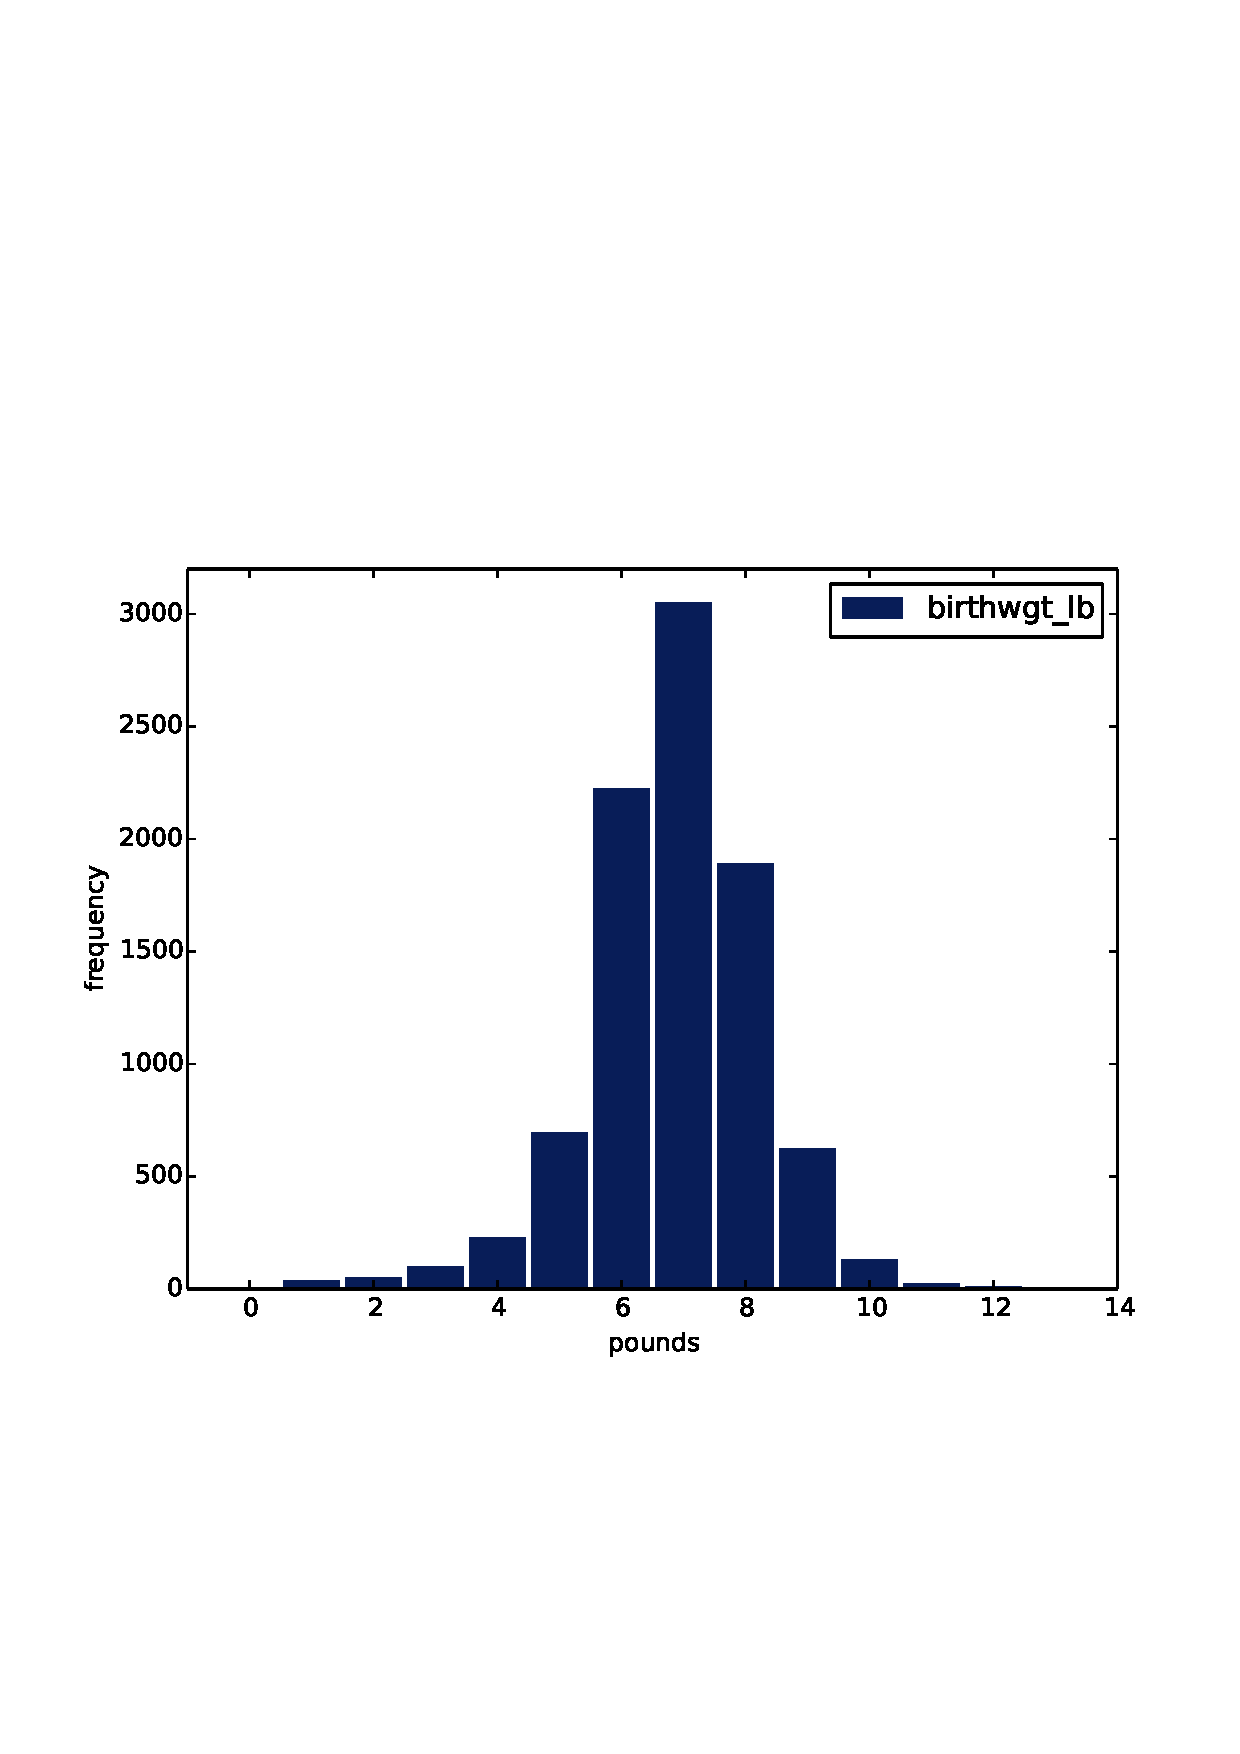
\includegraphics[height=2.5in]{figs/first_wgt_lb_hist.pdf}}
\caption{출생체중 파운드 히스토그램.}
\label{first_wgt_lb_hist}
\end{figure}

이 책에서 저자는 {\tt thinkplot.py} 모듈을 작성해서 Hists를 그리는 함수와 
{\tt thinkstats2.py}에 정의된 객체를 제공한다. {\tt pyplot}에 기반하고 있고 
{\tt matplotlib} 패키지의 일부다. 
{\tt matplotlib}을 설치하는 방법은 ~\ref{code}을 참조하세요.

\index{thinkplot}
\index{matplotlib}

{\tt thinkplot}으로 {\tt hist}를 그리기 위해서 다음을 시도해 보세요.

\index{Hist}

\begin{verbatim}
>>> import thinkplot
>>> thinkplot.Hist(hist)
>>> thinkplot.Show(xlabel='value', ylabel='frequency')
\end{verbatim}

\url{http://greenteapress.com/thinkstats2/thinkplot.html} 웹사이트에서
{\tt thinkplot}에 대한 문서를 참조할 수 있다.

\begin{figure}
% first.py
\centerline{\includegraphics[height=2.5in]{figs/first_wgt_oz_hist.pdf}}
\caption{출생체중 온스 히스토그램.}
\label{first_wgt_oz_hist}
\end{figure}


\section{NSFG 변수}

이제 NSFG에 있는 데이터로 다시 돌아가자. 이장에 있는 코드는 {\tt first.py}다. 
코드를 다운로드하고 작업에 대한 정보는 ~\ref{code} 장을 참조하라.

새로운 데이터셋을 가지고 작업을 시작할 때, 한번에 하나씩 사용하려는 변수를 탐색하길 제안한다. 
시작하는 좋은 방법은 히스토그램을 그려보는 것이다.

\index{히스토그램 (histogram)}


~\ref{cleaning}에서 {\tt agepreg}를 백분년에서 년단위로 변환했고,
\verb"birthwgt_lb"와 \verb"birthwgt_oz"을 조합해서 \verb"totalwgt_lb" 한 단위량으로 만들었다.
이번 절에서 히스토그램의 몇가지 기능을 시연하기 위해서 이 변수들을 사용한다.


\begin{figure}
% first.py
\centerline{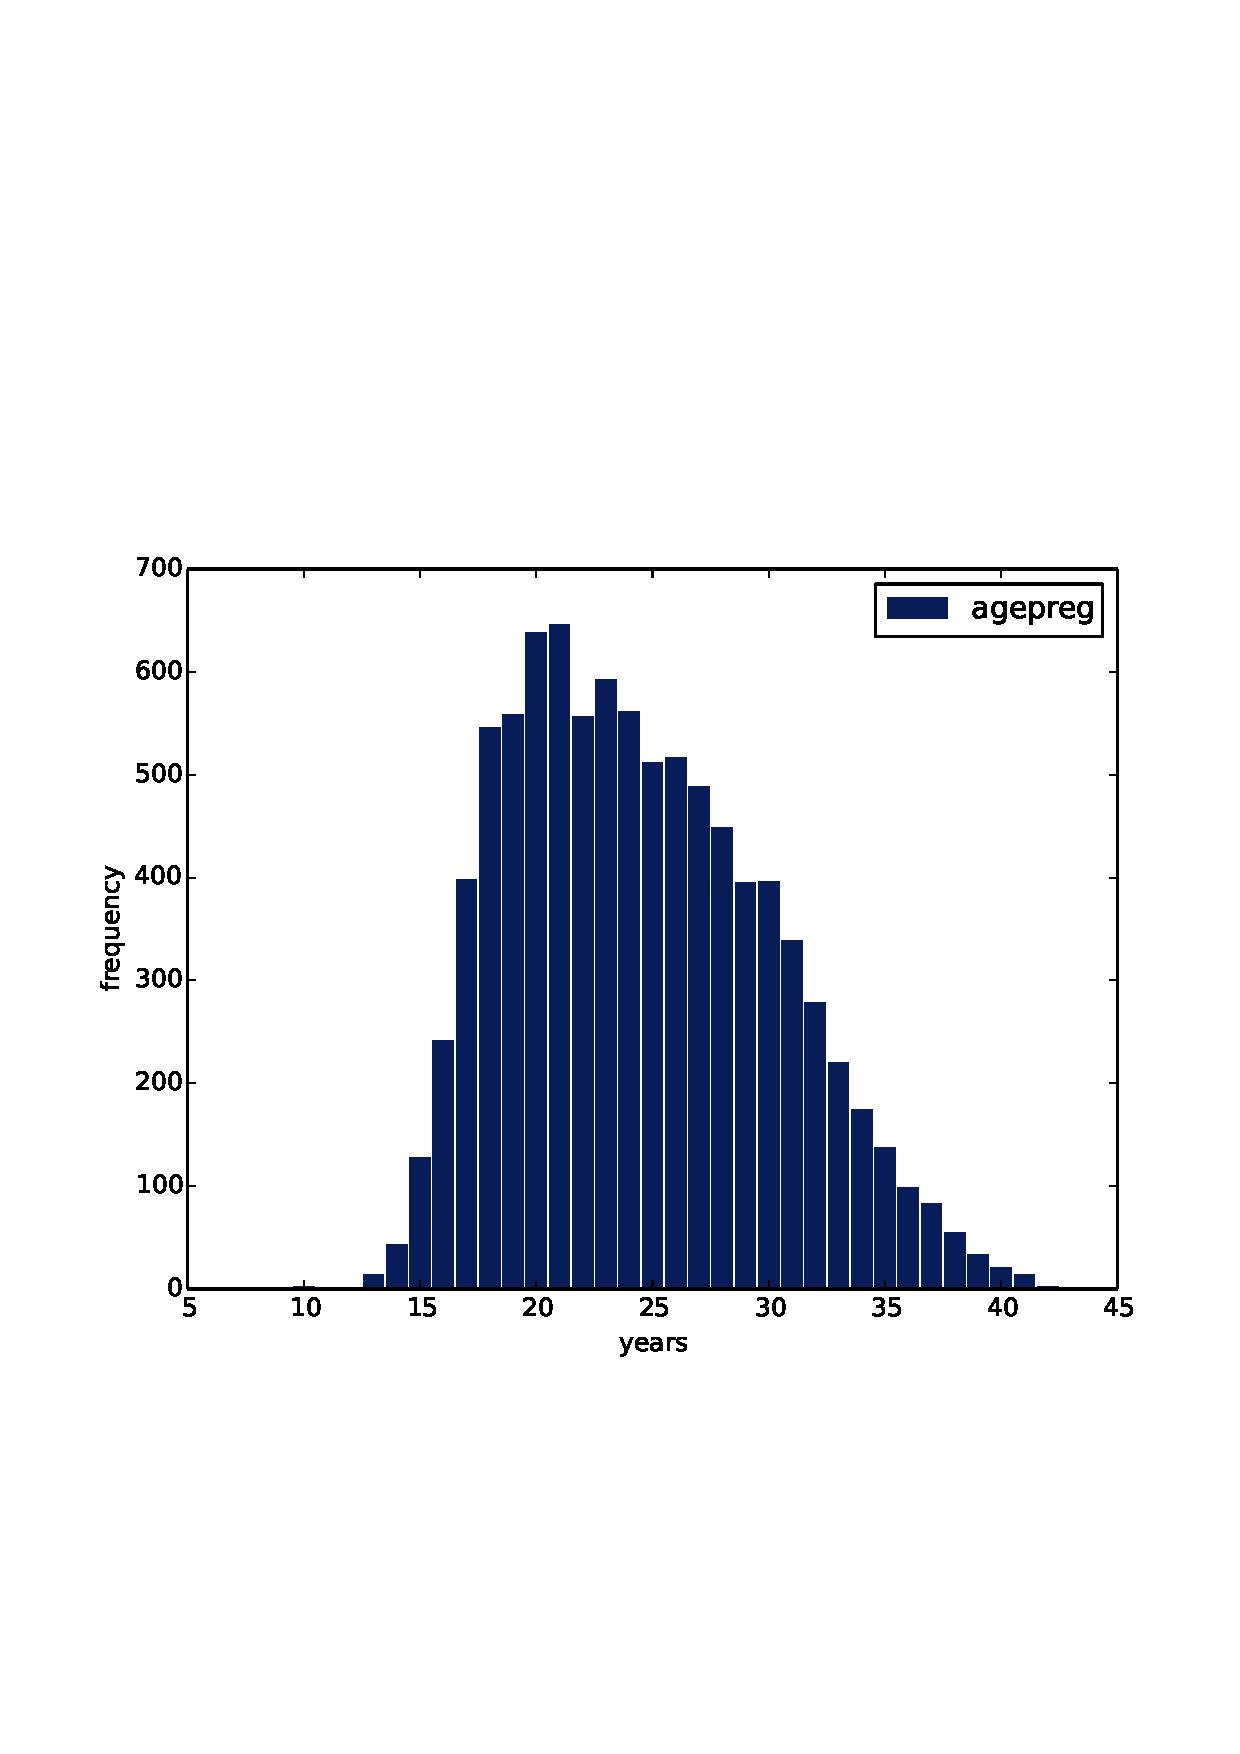
\includegraphics[height=2.5in]{figs/first_agepreg_hist.pdf}}
\caption{임신 종료시점 산모연령 히스토그램.}
\label{first_agepreg_hist}
\end{figure}

데이터를 읽고, 정상 출산에 대한 레코드를 선택해서 시작해보자.

\begin{verbatim}
    preg = nsfg.ReadFemPreg()
    live = preg[preg.outcome == 1]
\end{verbatim}

꺾쇠 표현식은 부울 시리즈(boolean Series)로 데이터프레임에서 행을 선택하고 새로운 데이터프레임을 반환한다. 다음에 정상출산에 대한 \verb"birthwgt_lb" 히스토그램을 생성하고 플롯해서 그려낸다.

\index{데이터프레임 (DataFrame)}
\index{시리즈 (Series)}
\index{Hist}
\index{꺾쇠 연산자 (bracket operator)}
\index{부울 (boolean)}

\begin{verbatim}
    hist = thinkstats2.Hist(live.birthwgt_lb, label='birthwgt_lb')
    thinkplot.Hist(hist)
    thinkplot.Show(xlabel='pounds', ylabel='frequency')
\end{verbatim}

Hist에 인자가 판다스 시리즈일 때, {\tt nan} 값은 탈락한다. 
{\tt label}은 문자열로 Hist가 그려질 때 범례에 나타난다. 

\index{판다스 (pandas)}
\index{시리즈 (Series)}
\index{thinkplot}
\index{NaN}

\begin{figure}
% first.py
\centerline{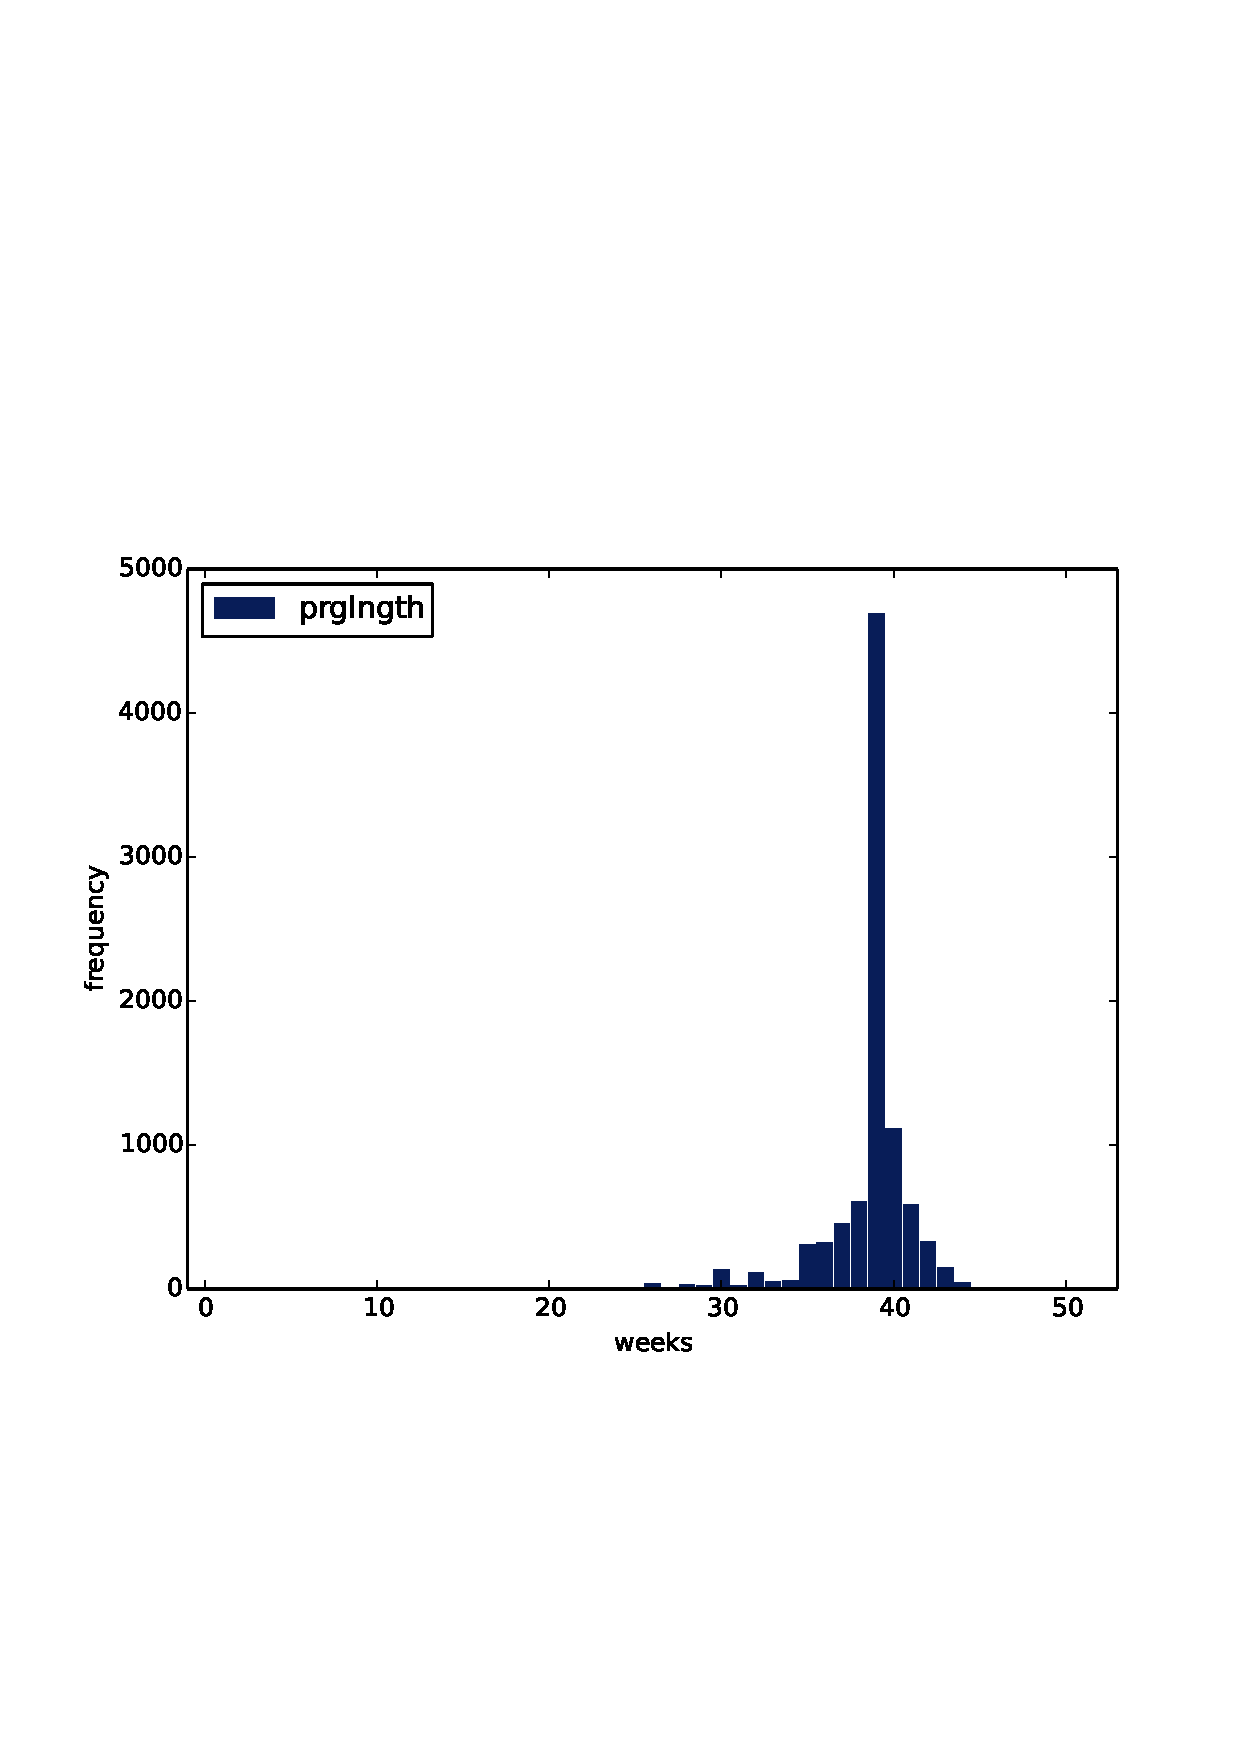
\includegraphics[height=2.5in]{figs/first_prglngth_hist.pdf}}
\caption{임신기간(주별) 히스토그램.}
\label{first_prglngth_hist}
\end{figure}

그림~\ref{first_wgt_lb_hist}가 결과를 보여준다.
가장 많이 관찰되는 값을 {\bf 최빈값(mode)}이라고 하고 이 경우에 7 파운드다. 
분포는 근사적으로 종모양인 {\bf 정규(normal)} 분포 모양으로 
{\bf 가우스(Gaussian)} 분포라고도 한다. 하지만, 순수 정규분포와 달리,
분포가 비대칭이다; 오른쪽보다 왼쪽으로 좀더 확장된 {\bf 꼬리(tail)}가 있다.


그림~\ref{first_wgt_oz_hist}은 변수 \verb"birthwgt_oz"의 히스토그램으로 출생 체중의 온스 부분이다. 
이론적으로 분포가 {\bf 균등(uniform)}하길 기대한다; 즉, 모든 값이 동일한 빈도를 가져야 한다.
사실 0 이 다른 값과 비교하여 좀더 흔하고, 1과 15는 좀더 흔하지 않은데, 아마도 이유는 응답자가 정수값에 가까운 출생 체중을 반올림한것으로 추측한다.

\index{출생 체중 (birth weight)}
\index{체중 (weight)!출생 (birth)}

그림~\ref{first_agepreg_hist}은 \verb"agepreg"의 히스토그램으로 임신 말기 산모 나이다.
분포는 대략 종모양이지만, 이 사례의 경우 꼬리가 좀더 왼쪽보다 오른쪽으로 뻗여나갔다. 
대부분의 산모는 20대이지만 30대도 적은 수지만 존재한다.

 
그림~\ref{first_prglngth_hist}은 \verb"prglngth"의 히스토그램으로 주간(week) 단위 임신기간이다.
가장 흔한 값은 39주다. 외쪽 꼬리가 오른쪽 꼬리보다 길다; 조산 신생아가 일반적이지만,
임신기간이 43주를 넘어가지는 않고, 만약 의사가 판단하기에 필요하다면 임신기간에 관여하는 것이 일반적이다.

\index{임신 기간 (pregnancy length)}


\section{특이점 (Outliers)}

히스토그램을 보면, 가장 흔한 값과 분포 모양을 식별하기는 쉽다. 하지만, 드문 값이 항상 눈에 잘 뜨이지는 않는다.
\index{히스토그램 (histogram)}

계속 진행하기 전에, {\bf 특이점 (outliers)}을 점검하는 것이 좋은 생각이다. 특이점은 이상치라고 불리는 극단값으로 측정과 기록에서 오류일 수도 있고, 드분 사건의 정확한 기록일 수도 있다.

\index{특이점 (outlier)}

Hist는 {\tt Largest}, {\tt Smallest} 메쏘드를 제공하는데, 정수 {\tt n}을 받아 히스토그램에서 최대값과 최소값 {\tt n}개를 반환한다.

\index{Hist}

\begin{verbatim}
    for weeks, freq in hist.Smallest(10):
        print(weeks, freq)
\end{verbatim}

정상 출산에 대한 임신기간 리스트에서 가장 작은 최소값 10개는 {\tt [0, 4, 9, 13, 17, 18, 19, 20, 21, 22]}이다. 10 주보다 적은 값은 확실한 오류다; 가장 그럴듯한 설명은 아마도 결과를 올바르게 코드화하지 못한 것이다. 30주 이상되는 값은 아마도 적합하다. 10주에서 30주 사이의 값은 확실하다고 하기가 어렵다; 몇몇 값은 아마도 오류지만 몇몇은 미숙아를 나타낸다.

\index{임신 기간 (pregnancy length)}

범위의 반대편에서 가장 큰 값은 다음과 같다.

%
\begin{verbatim}
weeks  count
43     148
44     46
45     10
46     1
47     1
48     7
50     2
\end{verbatim}

만약 임신기간이 42주를 넘어가면 대부분의 의사는 유도분만(induced labor)을 추천한다.
그래서 몇몇 긴 임신기간값은 놀라움을 준다. 특히, 임신 50주는 의학적으로 가능하지 않아 보인다.

특이점을 다루는 가장 좋은 방법은 ``특정 분야의 전문 지식(domain knowledge)''에 달려있다; 즉, 데이터 출처와 데이터가 의미하는 바에 대한 정보. 그리고 어떠한 분석방법을 수행할지에 달려있다.

\index{특이점 (outlier)}

이번 예제에서, 동기 부여 질문은 첫번째 아이가 일찍 (혹은 늦게) 태어나는 경향이 있느냐는 것이다.
사람들이 이 질문을 할 때, 대체로 전체 임신기간에 관심이 있다. 그래서, 이번 분석에서는 27주 이상이 되는 
임신에 초점을 맞출 것이다. 


\section{첫번째 아이 (First babies)}

첫째 아이와 나머지 아이에 대한 임신 기간 분포를 이제 비교할 수 있다.
{\tt birthord} 변수를 사용해서 정상 출산 데이터프레임을 나누고 히스토그램을 연산해서 그린다.

\index{데이터프레임 (DataFrame)}
\index{Hist}
\index{임신 기간 (pregnancy length)}

\begin{verbatim}
    firsts = live[live.birthord == 1]
    others = live[live.birthord != 1]

    first_hist = thinkstats2.Hist(firsts.prglngth)
    other_hist = thinkstats2.Hist(others.prglngth)
\end{verbatim}

그리고 나서, 동일 축에 히스토그램을 플롯하여 그린다.

\begin{verbatim}
    width = 0.45
    thinkplot.PrePlot(2)
    thinkplot.Hist(first_hist, align='right', width=width)
    thinkplot.Hist(other_hist, align='left', width=width)
    thinkplot.Show(xlabel='weeks', ylabel='frequency')
\end{verbatim}

{\tt thinkplot.PrePlot} 함수는 그래프를 그리려고하는 히스토그램 갯수를 인자로 받는다;
인자 정보를 이용해서 적절한 색깔 집합을 선택할 수 있다.

\index{thinkplot}

\begin{figure}
% first.py
\centerline{\includegraphics[height=2.5in]{figs/first_nsfg_hist.pdf}}
\caption{임신기간 히스토그램.}
\label{first_nsfg_hist}
\end{figure}

{\tt thinkplot.Hist}는 {\tt align='center'}을 기본값으로 사용해서 
각 막대는 값에 대해서 중앙에 위치한다. 그림에서는 {\tt align='right'}와 {\tt align='left'}를
사용해서 각 값의 양쪽으로 해당 막대를 위치시켰다.
\index{Hist}

{\tt width=0.45} 옵션값으로, 두 막대의 전체 넓이는 0.9로, 각 막대페어 간에 약간 공백을 두었다.

마지막으로, 축을 조정해서 27주와 46주 사이 데이터만 보이게 만들었다. 
그림~\ref{first_nsfg_hist}이 지금까지의 결과를 보여준다.
\index{임신 기간 (pregnancy length)}
\index{기간 (length)!임신 (pregnancy)}

히스토그램은 최빈값을 즉시 명확하게 보여준다는 점에서 유용하다.
하지만, 두 분포를 비교하는데는 가장 좋은 선택이 되지는 못하다. 
이번 예제에서 ``첫째가 아닌 아이''보다 ``첫째 아이'' 숫자가 더 적다. 
그래서, 히스토그램에서 명백한 차이는 표본크기에서 나온다. 다음 장에서 확률질량함수(probability mass functions)를 사용해서
이 문제를 다뤄본다. 


\section{분포 요약하기}
\label{mean}

히스토그램은 표본을 완전히 기술하는 분포다; 즉, 히스토그램이 주어진다면 (순서대로는 할 수 없지만) 표본에 있는 값을 재구성할 수 있다.

만약 분포에 대한 자세한 사항이 중요하다면, 히스토그램으로 표현하는 것이 필요할지도 모른다.
하지만, 종종 기술 통계량 몇개로 분포를 요약할 때도 있다.

보고하는데 사용되는 특성치 몇개는 다음과 같다.

\begin{itemize}

\item 중심경향성 (central tendency): 
값들이 특정한 점을 주심으로 군집하는 경향이 있는가?
\index{중심경향성 (central tendency)}

\item 모드 (modes): 하나 이상 군집(cluster)이 있는가?
\index{모드 (mode)}

\item 퍼짐 (spread): 값들에 얼마나 많은 변동이 있는가?
\index{퍼짐 (spread)}

\item 꼬리 (tails): 모드(최빈값)에서 멀어질 때, 확률이 얼마나 빨리 떨어지는가?
\index{꼬리 (tail)}

\item 특이점 (outliers): 모드(최빈값)에서 멀리 떨어진 극단값이 있는가?
\index{특이점 (outlier)}

\end{itemize}

상기 질문에 대답하도록 설계된 통계량이 {\bf 요약통계 (summary statistics)}다.
지금까지 가장 흔한 요약통계는  {\bf 평균(mean)}으로 분포의 중심경향성을 기술하는 의도가 있다.
\index{평균 (mean)} 
\index{평균 (average)} 
\index{요약통계 (summary statistic)}

각 값이 $x_i$인 {\tt n}개 표본이 있다면, 평균 $\xbar$는 값을 합한 뒤에 표본갯수로 나눈 것이다;
다른 말로, 
%
\[ \xbar = \frac{1}{n} \sum_i x_i \]
%

``평균 (mean)''와 ``평균(average)''은 때때로 상호호환적으으로 사용된다. 하지만 다음과 같이 이 책에서 구별한다.


\begin{itemize}

\item 표본 ``평균 (mean)''은 앞선 공식으로 계산되는 요약 통계다.

\item ``평균 (average)''은 중심경향성을 기술하려고 선택하는 다수 요약통계량 중 하나다.
\index{중심 경향성 (central tendency)}

\end{itemize}

때때로 평균(mean)은 값들의 집합을 잘 기술한다. 예를 들어, 사과는 거의 크기가 동일하다. (최소한 마트에서 팔리는 사과는 그렇다.)
그래서, 사과 6개를 사고, 전체 무게가 3 파운드라면, 사과 각각은 0.5 파운드라고 주장하는 것은 일리있는 요약이 된다. 

\index{무게 (weight)!호박 (pumpkin)}

하지만, 호박은 좀더 다양하다. 텃밭에서 호박 몇종을 기른다고 가정하자.
어느날 1 파운드 장식용 호박 3개, 3 파운드 호박파이용 호박 2개, 그리고 519 파운드 대서양 거인 호박 한개를 수확했다.
표본 평균은 100 파운드다. 하지만, ``텃밭에 호박 평균 무게는 100 파운드''라고 말한다면 오도할 수 있다.
호박 무게에 대해서 전형적인 호박이 없기 때문에 유의미한 평균은 없다.

\index{호박 (pumpkin)}


\section{분산 (Variance)}
\index{분산 (variance)}

호박 무게를 요약하는 단 하나의 숫자가 없다면, 숫자 두개로 좀더 잘 할 수 있다; 평균(meand)과 
{\bf 분산 (variance)}.

분산은 분포의 변동(variability)과 퍼짐(spread)을 기술하려는 요약통계다. 
값들의 집합에 대한 분산은 다음과 같다.

%
\[ S^2 = \frac{1}{n} \sum_i (x_i - \xbar)^2 \]
%

$x_i - \xbar$ 항은 ``평균으로부터 편차(deviation from the mean)''라고 하고,
분산은 평균제곱편차다. 분산의 제곱근($S$)을 {\bf 표준편차 (standard deviation)}라고 한다.
\index{편차 (deviation)}
\index{표준편자 (standard deviation)}

이전에 경험이 있다면, 분모에 {\tt n} 대신에 $n-1$로 분산을 계산하는 공식을 봤을 것이다.
이 통계치는 표본을 사용해서 모집단 분산을 추정하는데 사용된다. 이것에 대해서는 나중에 ~\ref{estimation}장에서 
다시 다룰 것이다.
\index{표본 분산 (sample variance)}

판다스 자료구조는 평균, 분산, 표준편차를 계산하는 메쏘드를 제공한다.
\index{판다스 (pandas)}

\begin{verbatim}
    mean = live.prglngth.mean()
    var = live.prglngth.var()
    std = live.prglngth.std()
\end{verbatim}

모든 정상 분만에 대해서, 평균 임신기간은 38.6주, 표준편차는 2.7주로 의미하는 바는 일반적으로 2-3주 편차가 있다는 것이다.
\index{임신 기간 (pregnancy length)}

임신 기간의 분산은 7.3으로 해석하기가 여렵다. 특히, 단위가 주$^2$, 즉 ``주 제곱''이다.
분산은 몇몇 계산에서는 유용하지만, 좋은 요약통계는 아니다.


\section{효과 크기 (Effect size)}
\index{효과 크기 (effect size)}

{\bf 효과 크기(effect size)}는 효과의 크기를 기술하려는 요약 통계다. 예를 들어,
두 집단간에 차이를 기술하기 위해서 평균값의 차이는 명확한 한가지 선택이 된다.
\index{효과 크기 (effect size)}

첫째 아이에 대한 평균 임신기간은 38.601; 첫째를 제외한 아이들의 평균 임신기간은 38.523이다. 
차이는 0.078주가 되고, 시간으로는 13시간이다. 전형적인 임신기간에 대한 일부분으로 보면, 차이는 약 0.2\%가 된다.
\index{임신 기간 (pregnancy length)}

만약 추정치가 정확하다고 가정하면, 이와 같은 차이는 실질적인 중요성은 없다.
사실, 대규모 임신사례를 관찰하지 않고 누구도 이와 같은 차이를 인지할 것 같지는 않다.
\index{효과 크기 (effect size)}

효과의 크기를 전달하는 또 다른 방법은 집단간(between groups)의 차이를 집단내(within groups) 변동성과 비교하는 것이다. 코헨(Cohen) $d$가 이러한 의도를 가진 통계량이다; 다음과 같이 정의된다.

%
\[ d = \frac{\bar{x_1} - \bar{x_2}}{s}  \]
%

$\bar{x_1}$와 $\bar{x_2}$은 집단 평균값이고, $s$는 ``합동 표준편차(pooled standard deviation)''다.
코헨(Cohen) $d$를 계산하는 파이썬 코드가 다음에 있다.

\index{표준편차 (standard deviation)!합동 (pooled)}

\begin{verbatim}
def CohenEffectSize(group1, group2):
    diff = group1.mean() - group2.mean()

    var1 = group1.var()
    var2 = group2.var()
    n1, n2 = len(group1), len(group2)

    pooled_var = (n1 * var1 + n2 * var2) / (n1 + n2)
    d = diff / math.sqrt(pooled_var)
    return d
\end{verbatim}

이 예제애서, 평균값의 차이는 0.029 표준편차로 크지 않다. 이러한 관점에서 본다면,
남성과 여성의 키 차이는 약 1.7 표준편차다.(\url{https://en.wikipedia.org/wiki/Effect_size} 참조)


\section{결과 보고하기}

첫째 아이와 첫째가 아닌 아이간에 임신 기간(만약 차이가 있다면)에 
차이를 기술하는 몇가지 방법을 살펴봤다.
\index{임신 기간 (pregnancy length)}

질문은 누가 질문을 하느냐에 달려있다. 과학자는 아무리 작더라도 존재하는 (실제) 차이에 관심이 있을지 모른다. 의사는 단지 {\bf 임상적으로 유의한 (clinically significant)} 효과에만 관심을 둘 수 있다; 즉, 치료결정에 영향을 주는 차이. 임신한 여성은 늦게 혹은 빨리 출산할 확률 같은 본인에게 관련된 결과에만 관심이 있을 수 있다. 

\index{임상적으로 유의한 (clinically significant)}
\index{유의한 (significant)}

어떻게 결과를 보고할지도 또한 목적에 달려있다. 만약 효과의 중요성을 시연하려고 한다면,
차이를 강조하는 요약통계량을 선택할 수도 있다. 만약 환자를 안심시키고자 한다면, 차이를 염두에 둔 통계량을 선택할지도 모른다. 

물론, 본인의 결정은 또한 전문가 윤리에 따라야만 한다. 설득하려고 한다면 괜찮다; 
스토리를 명확하게 전달하는 시각화 도구와 통계 보고서를 설계{\em 해야만 한다.}
하지만, 또한 보고서를 정직하게 만들고, 불활실성과 한계를 인정하는데도 최선을 다해야 한다.

\index{윤리 (ethics)}


\section{연습 문제}

\begin{exercise}
이번 장의 결과에 기반해서, 첫번째 아이 출산이 늦은가에 관해서 배운 것을 요약하도록 요청받는다고 가정하자.

9시 뉴스에 나온다면, 어떤 요약 통계량을 사용해야 할까?
불안해 하는 환자를 안심시키려면 어떤 요약 통계량을 사용해야 할까?

\index{Adams, Cecil}
\index{Straight Dope, The}

마지막으로, {\it 진실한 정보(The Straight Dope)} (\url{http://straightdope.com})의 저자
세실 아담스(Cecil Adams)라고 상상하자. 여러분의 일은 ``첫째 아이가 늦게 태어나는가?'' 질문에 대답하는 것이다.
분명하고, 정확하고, 정직하게 질문에 답하는데 이번 장에서 나온 결과를 사용해서 한 문단으로 작성하시오.
\index{윤리}

\end{exercise}

\begin{exercise}
다운로드받은 저장소에서, \verb"chap02ex.ipynb" 라는 이름의 파일을 찾아서 연다.
일부 셀이 이미 채워져 있고, 채워진 셀은 실행해야 한다.
다른 셀은 연습문제로 명령어를 넣어 주어야 된다.
지침을 따라서 정답을 채워넣으세요.

연습문제에 대한 해답은 \verb"chap02soln.ipynb" 파일에 나와 있다.

\end{exercise}

다음 연습문제로, {\tt chap02ex.py} 이름으로 파일을 생성하시오.
\verb"chap02soln.py" 파일에 정답이 나와있다.

\begin{exercise}
분포 최빈값(mode)은 가장 빈번하게 나오는 값이다; 
\url{http://wikipedia.org/wiki/Mode_(statistics)}을 참조한다.  
Hist를 입력값으로 받아서 가장 빈번하게 나오는 값을 반환하는 함수 
{\tt Mode}를 작성하시오.

\index{최빈값}
\index{Hist}

좀더 도전적인 연습문제로, {\tt AllModes}라는 함수를 작성한다.
빈도수를 내림차순으로 정렬하는 값-빈도를 짝지은 목록으로 반환한다.
\index{빈도}
\end{exercise}

\begin{exercise}
변수 \verb"totalwgt_lb"을 사용해서, 첫번째 아이가 다른 아이들보다 더 가벼운지
더 무거운지 조사하시오. 집단 사이 차이를 정량화하는데 코헨 $d$ (Cohen's $d$)를 계산한다.
임신 기간에 차이와 어떻게 비교가 되는가?
\index{임신 기간}
\end{exercise}


\section{용어사전}

\begin{itemize}

\item 분포 (distribution): 표본에 나타나는 값과 개별 값의 빈도
\index{분포 (distribution)}

\item 히스토그램 (histogram): 값에서 빈도로 매핑, 혹은 매핑을 보여주는 그래프.
\index{히스토그램 (histogram)}

\item 빈도 (frequency): 표본에서 값이 나타나는 횟수.
\index{빈도 (frequency)}

\item 최빈값 (mode): 표본에서 가장 빈도가 높은 값 혹은 가장 빈도가 높은 값중의 하나.
\index{최빈값 (mode)}

\item 정규분포 (normal distribution): 이상적인 종모양 분포; 가우스 분포로도 알려져 있다.
\index{가우스 분포 (Gaussian distribution)}
\index{정규분포 (normal distribution)}

\item 균등분포 (uniform distribution): 모든 값이 동일한 본도를 갖는 분포.
\index{균등분포 (uniform distribution)}

\item 꼬리 (tail): 가장 높고 가장 낮은 극단에 있는 분포 부분.
\index{꼬리 (tail)}

\item 중심경향성 (central tendency): 표본 혹은 모집단 특성치; 직관적으로 평균 혹은 전형적인 값.
\index{중심경향성 (central tendency)}

\item 특이점 (outlier): 중심경향성에서 떨어진 값.
\index{특이점 (outlier)}

\item 퍼짐 (spread): 분포에 있는 값들이 얼마나 퍼져있는지에 대한 측정.
\index{퍼짐 (spread)}

\item 요약통계 (summary statistic): 
중심경향성 혹은 퍼짐같이 분포의 일부 측면을 정량화하는 통계치.
\index{요약통계 (summary statistic)}

\item 분산 (variance): 퍼짐을 정량화하는데 종종 사용되는 요약통계.
\index{분산 (variance)}

\item 표준편차 (standard deviation): 분산의 제곱근으로 또한 퍼짐을 측정하는데 사용된다.
\index{표준편차 (standard deviation)}

\item 효과 크기 (effect size): 집단간의 차이처럼 효과 크기를 정량화하는 요약통계.
\index{효과 크기 (effect size)}

\item 임상적으로 유의한 (clinically significant): 집단간 차이처럼, 실제로 연관있는 결과. 
\index{임상적으로 유의한 (clinically significant)}

\end{itemize}




\chapter{확률 질량 함수}
\index{확률 질량 함수 (probability mass function)}

이번 장에서 사용되는 코드는 {\tt probability.py}에 있다.
코드를 다운로드하고 작업하는 것에 대한 정보는 ~\ref{code}을 참조한다.

\section{Pmf}
\index{Pmf}

분포를 표현하는 또다른 방식은 {\bf 확률 질량 함수(probability mass function)} (PMF)로 각 값을 확률로 매핑한다. 
{\bf 확률(probability)}은 표본 크기 {\tt n}의 일부로서 표현되는 빈도다. 
빈도에서 확률을 얻기 위해서, {\tt n}으로 나누는데 이를 {\bf 정규화(normalization)}라고 부른다.

\index{빈도 (frequency)}
\index{확률 (probability)}
\index{정규화 (normalization)}
\index{PMF}
\index{확률 질량 함수 (probability mass function)}

Hist가 주어지면, 각 값에 확률값을 매핑하는 딕셔너리를 만들 수 있다.
\index{Hist}

%
\begin{verbatim}
n = hist.Total()
d = {}
for x, freq in hist.Items():
    d[x] = freq / n
\end{verbatim}
%

혹은 {\tt thinkstats2}에서 제공하는 Pmf 클래스를 사용할 수도 있다.
Hist와 마찬가지로, Pmf 생성자는 판다스, 시리즈, 딕셔너리, Hist, 다른 Pmf 객체를 받을 수 있다.
다음에 간단한 리스트를 입력값으로 받는 예제가 있다.

%
\begin{verbatim}
>>> import thinkstats2
>>> pmf = thinkstats2.Pmf([1, 2, 2, 3, 5])
>>> pmf
Pmf({1: 0.2, 2: 0.4, 3: 0.2, 5: 0.2})
\end{verbatim}

Pmf는 정규화 과정을 거쳐 전체 확률값이 1이 된다.

Pmf와 Hist 객체는 많은 점에서 비슷하다; 사실, 공통 부모 클래스에서 많은 메쏘드를 상속받았다.
예를 들어, {\tt Values}와 {\tt Items} 메쏘드는 두 객체 모두에 동일한 방식으로 동작한다.
가장 큰 차이점은 Hist가 값을 정수형 계수기(integer counter)로 매핑한다는 것이고; 
Pmf는 값을 부동소수점 확률값으로 매핑한다는 것이다. 
\index{Hist}

값과 연관된 확률값을 조회하려면, {\tt Prob}를 사용한다.:
%
\begin{verbatim}
>>> pmf.Prob(2)
0.4
\end{verbatim}

꺾쇠 연산자도 동등한 기능을 한다.
\index{꺾쇠 연산자 (bracket operator)}

\begin{verbatim}
>>> pmf[2]
0.4
\end{verbatim}

기존 Pmf를 값과 연관되어 있는 확률값을 증가시킴으로써 변경할 수 있다.
%
\begin{verbatim}
>>> pmf.Incr(2, 0.2)
>>> pmf.Prob(2)
0.6
\end{verbatim}

혹은 확률에 일정량을 곱할 수도 있다.
%
\begin{verbatim}
>>> pmf.Mult(2, 0.5)
>>> pmf.Prob(2)
0.3
\end{verbatim}

만약 Pmf를 변경하면, 결과는 정규화되지 않을지도 모른다; 즉, 확률값을 다 합하면 1이 되지 않을지도 모른다.
확률값을 합한 결과를 반환하는데 사용되는 {\tt Total} 메쏘드를 호출해서 확인한다. 

%
\begin{verbatim}
>>> pmf.Total()
0.9
\end{verbatim}

다시 정규화하기 위해서, {\tt Normalize}를 호출한다:
%
\begin{verbatim}
>>> pmf.Normalize()
>>> pmf.Total()
1.0
\end{verbatim}

Pmf 객체는 {\tt Copy} 메쏘드를 제공하는데, 이를 통해서 원본에 영향을 주지않고, 사본을 만들고 변경 작업을 할 수 있다.
\index{Pmf}

이번 절에 표기법이 일관성을 갖지 않는 것처럼 보일지도 모르지만 체계가 있다;
Pmf를 클래스 명칭으로, pmf는 클래스의 인스턴스로, PMF는 확률질량함수에 대한 수학적 개념으로 각각을 표기하는데 사용한다.

\section{PMF 플롯으로 그리기}
\index{PMF}

{\tt thinkplot}은 Pmf 플롯을 그리는 두가지 방식을 제공한다.
\index{thinkplot}

\begin{itemize}

\item Pmf를 막대그래프로 그리기 위해서 {\tt thinkplot.Hist}을 사용한다.
만약 Pmf에 값의 개수가 작다면 막대그래프가 가장 유용한다.
\index{막대그래프 (bar plot)}
\index{그래프 (plot)!막대 (bar)}

\item 계단 함수로 Pmf를 그래프 그리기 위해서는, {\tt thinkplot.Pmf}을 사용할 수 있다.
만약 값이 많고, Pmf가 매끄럽다면(smooth) 탁월한 선택이 된다. 이 함수는 Hist 객체에서도 동작한다.
\index{선그래프 (line plot)}
\index{그래프 (plot)!선 (line)}
\index{Hist}
\index{Pmf}

\end{itemize}

추가로, {\tt pyplot}은 {\tt hist} 함수를 제공하는데 값(value) 시퀀스를 받아서
히스토그램을 계산하고, 그래프로 그린다.
Hist 객체를 사용하기 때문에, {\tt pyplot.hist}은 사용하지 않는다.
\index{pyplot}

\begin{figure}
% probability.py
\centerline{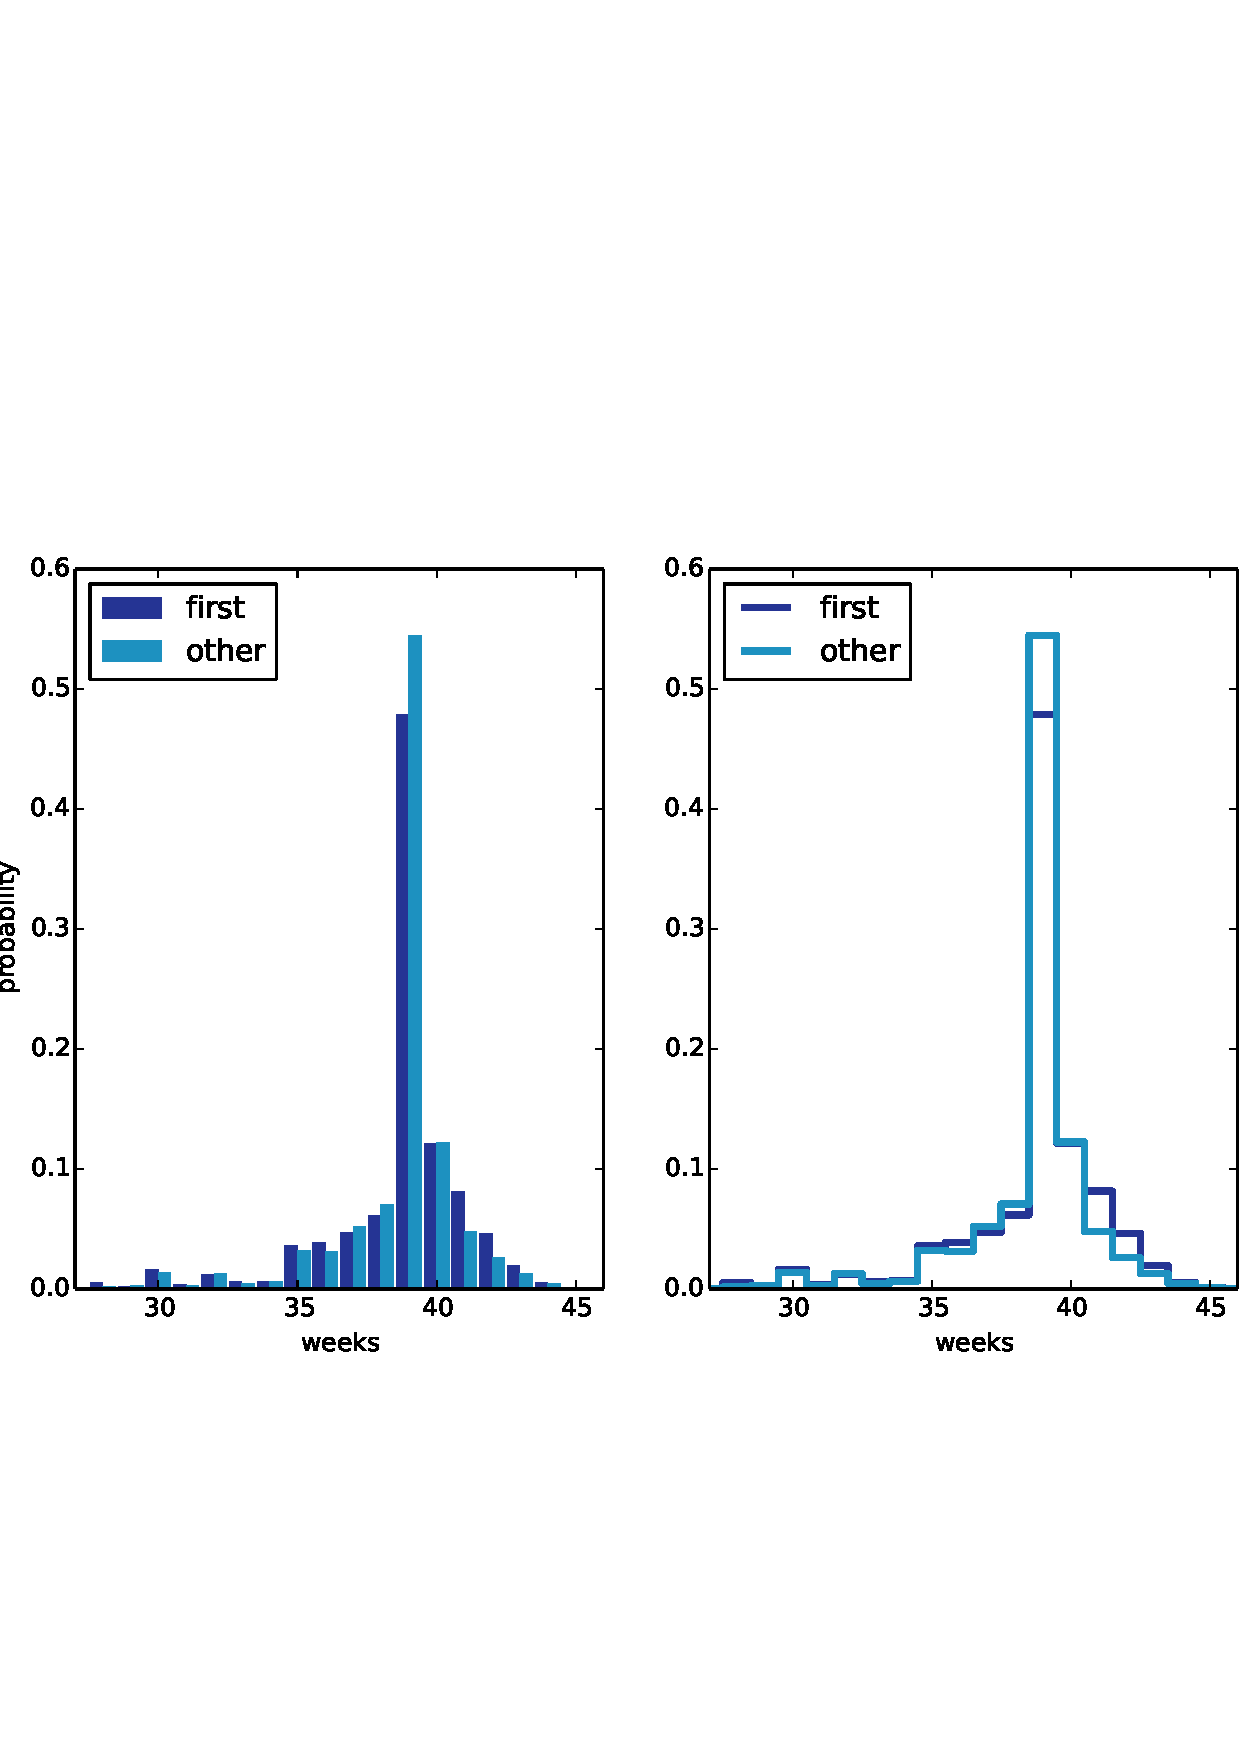
\includegraphics[height=3.0in]{figs/probability_nsfg_pmf.pdf}}
\caption{막대 그래프와 계단 함수를 사용하여, 첫째 아기와 첫째가 아닌 아기에 대한 임신기간 PMF.}
\label{probability_nsfg_pmf}
\end{figure}
\index{임신기간 (pregnancy length)}
\index{기간 (length)!임신 (pregnancy)}

그림~\ref{probability_nsfg_pmf}은 막대그래프(왼쪽)와 계단함수(오른쪽)를 사용해서 첫째 아이와 첫째가 아닌 아이에 대한
임신기간 PMF를 보여준다.
\index{임신기간 (pregnancy length)}

히스토그램 대신에 PMF 플롯을 그려서, 표본차이로 오도되지 않고 두 분포를 비교할 수 있다.
그림을 해석하면, 첫번째 아이는 다른 아이들보다 정시(39주차)에 출산하지 않고, 늦게(41, 42주차) 출산할 것 같다.

그림~\ref{probability_nsfg_pmf}을 생성하는 코드가 다음에 있다:

\begin{verbatim}
    thinkplot.PrePlot(2, cols=2)
    thinkplot.Hist(first_pmf, align='right', width=width)
    thinkplot.Hist(other_pmf, align='left', width=width)
    thinkplot.Config(xlabel='weeks',
                     ylabel='probability',
                     axis=[27, 46, 0, 0.6])

    thinkplot.PrePlot(2)
    thinkplot.SubPlot(2)
    thinkplot.Pmfs([first_pmf, other_pmf])
    thinkplot.Show(xlabel='weeks',
                   axis=[27, 46, 0, 0.6])
\end{verbatim}

{\tt PrePlot} 메쏘드는 옵션 매개변수 {\tt rows}와 {\tt cols}을 받아서 
그림 격자(grid)를 만드는데 이경우 한 행에 그림 두개를 넣는 격자가 된다.
첫번째 그림(왼쪽)은 {\tt thinkplot.Hist}을 사용해서 앞에서 봤던 Pmf를 화면에 출력한다. 

\index{thinkplot}
\index{Hist}

{\tt PrePlot}에 두번째 호출로 색깔 생성자를 초기화한다. 그리고 나서 
{\tt SubPlot}이 두번째 그림(오른쪽)으로 바꿔서, {\tt thinkplot.Pmfs}을 사용해서 Pmf를 화면에 출력한다.
{\tt axis}을 사용해서 그림 두개 모두 동일한 축(axis)에 놓여지도록 확실히 한다.
그림 두개를 비교하려고 한다면, 축을 통일하는 것이 좋다.


\section{다른 시각화 방법}
\label{visualization}

히스토그램과 PMF은 데이터를 탐색하고 패턴과 관계를 식별하는데 유용하게 사용된다. 데이터에서 무슨 정보가 담겨져있고, 어떻게 돌아가는지 아이디어를 얻게 된다면, 다음 단계는 최대한 깔끔하게 식별한 패턴화할 수 있는 시각화 설계하는 것이다. 

\index{탐색적 자료 분석 (exploratory data analysis)}
\index{시각화 (visualization)}

NSFG데이터에서 분포에서 가장 큰 차이는 모드(최빈치)에 있다. 그래서, 그래프에서 이 부분만을 확대하여 들여다보고, 차이를 강조하도록 자료를 변환하는 것이 의미가 있다.

\index{가족 성장 국가 조사 (National Survey of Family Growth)}
\index{NSFG}

\begin{verbatim}
    weeks = range(35, 46)
    diffs = []
    for week in weeks:
        p1 = first_pmf.Prob(week)
        p2 = other_pmf.Prob(week)
        diff = 100 * (p1 - p2)
        diffs.append(diff)

    thinkplot.Bar(weeks, diffs)
\end{verbatim}

상기 코드에서 {\tt weeks}가 임신주 범위다; {\tt diffs}는 퍼센트에서 두 PMF간 차이가 된다.  
그림~\ref{probability_nsfg_diffs}는 막대그래프로 결과를 보여준다.
그림이 패턴을 좀더 명확하게 한다: 첫째 아이는 임신 39주차에 덜 태어날 것 같고, 임신 41, 42주차에 더 태어날 것 같다.
\index{thinkplot}

\begin{figure}
% probability.py
\centerline{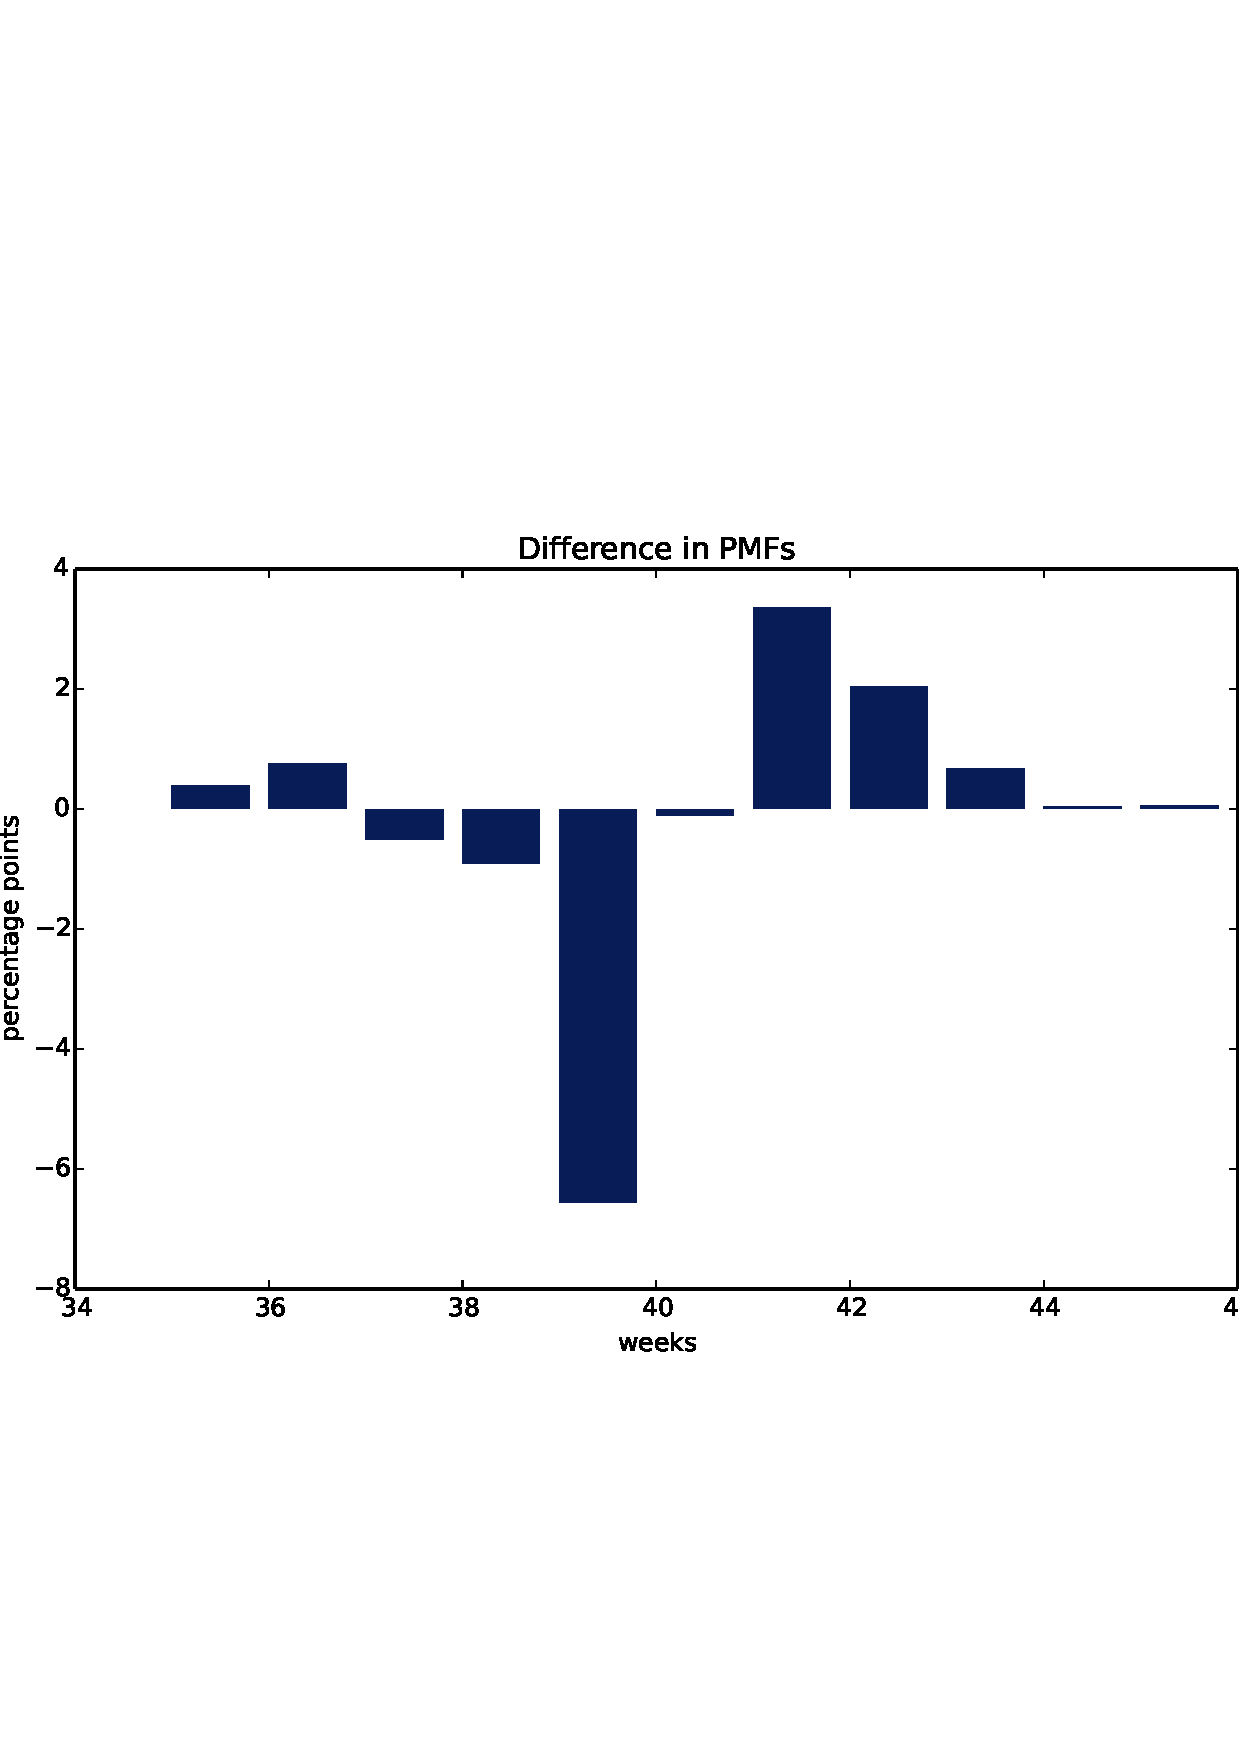
\includegraphics[height=2.5in]{figs/probability_nsfg_diffs.pdf}}
\caption{주별 백분율점(percentage point)으로 나타낸 차이.}
\label{probability_nsfg_diffs}
\end{figure}

지금까지 결론을 잠정적으로 내렸다. 동일한 데이터셋을 사용해서 명백하게 차이를 식별하고 나서 차이를 명확하게 만드는 시각화 방식을 선택했다. 효과 차이가 실질적인지 확실하다고 할 수는 없다; 확률변동(random variation)일 수도 있다. 나중에 이 문제를 다시 다룰 것이다.


\section{학급 크기 패러독스 (class size paradox)}
\index{학급 크기 (class size)}

진도를 더 나가기 전에, Pmf 객체를 가지고 할 수 있는 한가지 계산(computation)을 시연하고자 한다; 다음 예제를 ``학급 크기 패러독스(class size paradox)''라고 명명한다.
\index{Pmf}

많은 미국 대학에서, 학생대교수 비율은 약 10:1이 된다. 
하지만 종종 학생들이 평균 학급크기가 10보다 큰 것을 발견하고 놀라곤 한다.
불일치에 대한 두가지 이유가 있다.

\begin{itemize}

\item 학생들이 학기당 일반적으로 4--5 과목을 수강하지만, 교수는 1 혹은 2 교과목만 가르친다. 

\item 적은 학급 수업을 즐기는 학생 숫자는 적지만, 큰 학급 수업에 학생수는 많다.
\end{itemize}

첫 이유는 명확하지만, 두번째 이유는 다소 모호하다. 사례를 살펴보자. 대학에서 다음과 같은 학급 크기 분포로 한 학기에 65 교과목을 개설한다고 가정하자.

%
\begin{verbatim}
 size      count
 5- 9          8
10-14          8
15-19         14
20-24          4
25-29          6
30-34         12
35-39          8
40-44          3
45-49          2
\end{verbatim}

만약 학교 총장에게 평균 학급크기를 물어본다면, 총장은 PMF를 생성하고, 평균을 계산하고 나서 학급 평균 크기가 23.7이라고 보고한다. 다음에 코드가 있다.

\begin{verbatim}
    d = { 7: 8, 12: 8, 17: 14, 22: 4, 
          27: 6, 32: 12, 37: 8, 42: 3, 47: 2 }

    pmf = thinkstats2.Pmf(d, label='actual')
    print('mean', pmf.Mean())
\end{verbatim}

하지만, 학생집단을 대상으로 수업에 학생이 있는지 물어보고, 평균을 계산한다면, 평균 학급크기가 더 크다고 생각할 것이다. 얼마나 더 큰지 살펴보자.

먼저, 학생들이 관측한 분포를 계산하자. 여기서 각 학급 크기와 연관된 확률은 학급에 있는 학생으로 ``편의(bias)''가 있다.

\index{관측자 편의 (observer bias)}
\index{편의 (bias)!관측자 (observer)}

\begin{verbatim}
def BiasPmf(pmf, label):
    new_pmf = pmf.Copy(label=label)

    for x, p in pmf.Items():
        new_pmf.Mult(x, x)
        
    new_pmf.Normalize()
    return new_pmf
\end{verbatim}

각 학급 크기 {\tt x}마다, 확률값에 학급 크기를 관측한 학생수 {\tt x}를 곱한다. 결과는 편의분포를 나타내는 새로운 Pmf가 된다.

이제 실제와 관측된 분포 모두를 플롯 그래프로 그릴 수 있다.
\index{thinkplot}

\begin{verbatim}
    biased_pmf = BiasPmf(pmf, label='observed')
    thinkplot.PrePlot(2)
    thinkplot.Pmfs([pmf, biased_pmf])
    thinkplot.Show(xlabel='class size', ylabel='PMF')
\end{verbatim}

\begin{figure}
% probability.py
\centerline{\includegraphics[height=3.0in]{figs/class_size1.pdf}}
\caption{실제값과 학생이 관측한 값에 대한 학급크기 분포.}
\label{class_size1}
\end{figure}

그림~\ref{class_size1}은 결과를 보여준다. 편의된 분포에서 작은 학급은 더 작고, 큰 학급은 더 많다. 편의된 분포 평균은 29.1로 실제 평균값보다 약 25\%더 많다. 

이 연산을 거꾸로 하는 것도 또한 가능하다. 대학 학급 크기 분포를 알고자 한다고 가정하자. 하지만, 대학 총장으로부터 신뢰성 있는 자료를 얻을 수는 없다. 대안은 무작위 학생 표본을 골라 학급에 학생수가 얼마인지 설문하는 것이다.
\index{편의 (bias)! 오버샘플링 (oversampling)} 
\index{오버샘플링 (oversampling)}

결과는 앞선 살펴봤던 이유로 편의가 있을지 모르지만, 이것을 사용해서 실제 분포를 추정한다. 다음에 Pmf 불편의(unbiased) 함수가 있다. 

\begin{verbatim}
def UnbiasPmf(pmf, label):
    new_pmf = pmf.Copy(label=label)

    for x, p in pmf.Items():
        new_pmf.Mult(x, 1.0/x)
        
    new_pmf.Normalize()
    return new_pmf
\end{verbatim}

{\tt BiasPmf} 함수와 비슷하다; 유일한 차이점은 곱하는 대신에 각 확률값을 {\tt x}로 나눈다는 것이다.

\section{데이터프레임 인덱싱 (DataFrame indexing)}

\ref{dataframe} 절에서 판다스 데이터프레임을 읽고, 데이터프레임을 사용해서 데이터 열(칼럼)을 선택하고 변경했다. 
이제 행선택을 살펴보자.
NumPy 난수 행렬을 생성하고, 이것을 사용해서 데이터프레임으로 초기화한다.

\index{넘파이 (NumPy)}
\index{판다스 (pandas)}
\index{데이터프레임 (DataFrame)}

\begin{verbatim}
>>> import numpy as np
>>> import pandas
>>> array = np.random.randn(4, 2)
>>> df = pandas.DataFrame(array)
>>> df
          0         1
0 -0.143510  0.616050
1 -1.489647  0.300774
2 -0.074350  0.039621
3 -1.369968  0.545897
\end{verbatim}

초기 설정값(by default)으로 행과 열 모두 0에서 시작하는 숫자로 번호가 매겨진다. 하지만, 열이름을 지정할 수 있다.

\begin{verbatim}
>>> columns = ['A', 'B']
>>> df = pandas.DataFrame(array, columns=columns)
>>> df
          A         B
0 -0.143510  0.616050
1 -1.489647  0.300774
2 -0.074350  0.039621
3 -1.369968  0.545897
\end{verbatim}

행이름도 지정할 수 있다. 행이름 집합을 {\bf index}라고 한다; 
행이름 자체는 {\bf labels}이라고 한다.

\begin{verbatim}
>>> index = ['a', 'b', 'c', 'd']
>>> df = pandas.DataFrame(array, columns=columns, index=index)
>>> df
          A         B
a -0.143510  0.616050
b -1.489647  0.300774
c -0.074350  0.039621
d -1.369968  0.545897
\end{verbatim}

앞장에서 살펴보았듯이, 단순 인덱싱으로 열을 선택하면 시리즈를 반환한다.

\index{시리즈 (Series)}

\begin{verbatim}
>>> df['A']
a   -0.143510
b   -1.489647
c   -0.074350
d   -1.369968
Name: A, dtype: float64
\end{verbatim}

레이블(label)로 행을 선택하려면 {\tt loc} 속성을 사용하면 되고 시리즈를 반환한다.  

\begin{verbatim}
>>> df.loc['a']
A   -0.14351
B    0.61605
Name: a, dtype: float64
\end{verbatim}

레이블(label) 보다 행의 정수 위치정보를 알고 있다면, {\tt iloc}속성을 사용하고, 실행 결과로 시리즈를 반환한다.

\begin{verbatim}
>>> df.iloc[0]
A   -0.14351
B    0.61605
Name: a, dtype: float64
\end{verbatim}

또한 {\tt loc}는 레이블 리스트를 인자로 받고, 결과로 데이터프레임을 반환한다.

\begin{verbatim}
>>> indices = ['a', 'c']
>>> df.loc[indices]
         A         B
a -0.14351  0.616050
c -0.07435  0.039621
\end{verbatim}

마지막으로 레이블(label)로 행 범위를 선택하는데 슬라이스를 사용할 수 있다.

\begin{verbatim}
>>> df['a':'c']
          A         B
a -0.143510  0.616050
b -1.489647  0.300774
c -0.074350  0.039621
\end{verbatim}

혹은 정수 위치정보를 사용할 수도 있다.

\begin{verbatim}
>>> df[0:2]
          A         B
a -0.143510  0.616050
b -1.489647  0.300774
\end{verbatim}

어느 경우든지 관계없이 결과는 데이터프레임이 된다. 하지만 첫번째 결과는 슬라이스 끝값을 포함하지만, 두번째는 끝값을 포함하지 않는 것을 주목하라.
\index{데이터프레임 (DataFrame)}

저자 충고: 만약 행에 단순히 정수값이 아닌 레이블(label)이 있다면, 레이블을 일관되게 사용하고 정수 위치정보 사용을 피하라.


\section{연습 문제}
이번 연습문제 대한 해답은 \verb"chap03soln.ipynb" 파일과 
\verb"chap03soln.py" 파일에 담겨있다.

\begin{exercise}
만약 자녀에 대해서, 얼마나 많은 자녀가 있는지 묻는다면, 학급 크기 패러독스 같은 것이 나타난다. 많은 자녀를 갖는 가족이 표본에 더 잘 나타날 것 같고 자녀가 없는 가족이
표본에 나타날 가능성은 없다.

\index{관측자 편향}
\index{편향!관측자}

NSFG 응답자 \verb"NUMKDHH" 변수를 사용해서 
가구에서 18세 이하 자녀수에 대한 실제 분포를 생성하라.

이제 만약 자녀에 대해서, 18세 이하 (본인 포함) 얼마나 많은 자녀가 있는지 묻는다면,
보게될 편향된 분포를 계산하라.

실제 분포와 편향된 분포를 도식화하고 평균을 계산하라. 
출발장소로 \verb"chap03ex.ipynb" 파일을 사용할 수 있다.
\end{exercise}


\begin{exercise}
\index{평균 (mean)}
\index{분산 (variance)}
\index{PMF}

\ref{mean}~절에서 구성요소를 더해가고 $n$으로 나눠서 표본 평균을 계산했다.
만약 PMF가 주어지면, 여전히 평균을 계산할 수 있으나, 과정은 다소 차이가 난다:
%
\[ \xbar = \sum_i p_i~x_i \]
%
여기서, $x_i$는 PMF에 있는 유일한 값이고, $p_i=PMF(x_i)$.
마찬가지로, 다음과 같이 분산을 계산할 수 있다:
%
\[ S^2 = \sum_i p_i~(x_i - \xbar)^2\]
% 
Pmf 객체를 인자로 받아 평균과 분산을 계산하는 함수를 
{\tt PmfMean} 와 {\tt PmfVar} 으로 이름지어 작성하시오.
작성한 메쏘드를 테스트하기 위해서, Pmf에서 제공하는 
{\tt Mean}, {\tt Var} 메쏘드와 일치하는지 검사하라.
\index{Pmf}

\end{exercise}


\begin{exercise}
저자는 ``첫째 아이가 좀더 늦게 태어날 것 같은가?'' 라는 질문으로 시작했다.
이 질문을 다루는데, 아이 집단간에 평균에 차이를 계산했다.
하지만, {\em 동일 여성에 대해} 첫째 아이와 다른 아이 사이에 차이가 있을 수 있다는 가능성을 간과했다.

이 질문을 다루는데, 적어도 아이가 두명인 응답자를 선택하고 
쌍별 차이(pairwise difference)를 계산한다.
이 질문 구성이 다른 결과를 도출해 내는가?

힌트: {\tt nsfg.MakePregMap}을 사용한다.
\end{exercise}


\begin{exercise}
\label{relay}

대부분의 도보경주(foot race)에서 모든 사람이 같은 시간에 출발한다.
만약 빠른 주자라면, 초반 경주에서 많은 사람을 앞질러 간다.
하지만, 몇 마일 지난 후에 주위 모든 사람은 같은 속도록 달려간다.

\index{계주}

저자가 처음으로 장거리 (209마일) 계주를 뛰었을 때, 저자는 특이한 현상을 알아챘다:
저자가 다른 주자를 따라 잡았을 때, 저자는 통상 훨씬 더 빠르고,
또다른 주자가 저자를 따라 잡았을 때, 또다른 주자가 저자보다 훨씬 더 빠르다.

처음에, 저자는 선수속도 분포가 이봉이라고 생각했다;
즉, 속도가 느린 주자와 속도가 빠른 주자, 하지만 저자와 같은 속도는 소수.

그리고 나서, 저자가 학급크기 효과와 유사한 편향의 희생자임을 인식하게 되었따.
경주는 두가지 방식으로 일반적이 않다: 스태거드 스타트(Staggered Start)를 사용해서, 다른 시점에 팀을 지어 출발한다; 그래서 다른 수준의 능력을 갖는 주자가 많은 팀에 포함된다.

\index{편향!선택} \index{선택 편향}

결과적으로, 주자는 속도와 장소에 거의 관계없이 경주과정을 통해서 쭉 펼쳐지게 된다.
저자가 경주에 참가했을 때, 저자 주위 참가자는 (상당히) 경주에 참가한 임의 표본이다.

그래서, 편향은 어디서 나오는 것일까? 경주를 진행하는 동안, 저자가 경주자를 추월하고, 추월당하는 가능성은 속도 차이에 비례한다. 저자가 느린 주자를 따라잡을 것 같고, 
빠른 주자에 따라잡힐 듯 하다. 하지만, 같은 속도를 갖는 주자는 서로를 보지 못할 듯 하다.

{\tt ObservedPmf}로 불리는 함수를 작성한다.
작성한 함수는 주자 속도와 달리는 관측자의 속도에 대한 실제 분포를 나타내는 Pmf를 인자로 받고, 관측자가 본 경주자의 분포를 나타내는 새로운 Pmf를 반환한다.

\index{관측자 편향}
\index{편향!관측자}

작성한 함수를 테스트하는데, {\tt relay.py}를 사용할 수 있는데,
마이애미 Dedham에서 열린 10 킬로미터 제임스 조이스 경주(James Joyce Ramble)에서 
나온 결과를 읽고 각 주자의 속도를 mph로 변환한다.

만약 7.5 mph로 해당 집단 주자와 계주를 달린다면, 관측할 속도 분포를 계산하시오.
이 연습문제 대한 해답은 \verb"relay_soln.py"에 나와있다.
\end{exercise}


\section{용어사전}

\begin{itemize}

\item 확률질량함수 (Probability mass function, PMF): 값을 확률로 매핑하는 함수로 분포를 표현.
\index{PMF}
\index{확률질량함수 (probability mass function)}

\item 확률 (probability): 
표본크기의 일부로 표현되는 빈도수.
\index{빈도 (frequency)}
\index{확률 (probability)}

\item 정규화 (normalization): 
확률값을 얻기 위해서 표본 크기로 빈도수를 나누는 과정.
\index{정규화 (normalization)}

\item 인덱스 (index): 
판다스 데이터프레임에서, 인덱스는 행 레이블(label)을 포함하는 특별한 열(칼럼)이다.
\index{판다스 (pandas)}
\index{데이터프레임 (DataFrame)}

\end{itemize}


\chapter{누적분포함수}
\label{cumulative}

이번 장에서 사용되는 코드는 {\tt cumulative.py}에 있다.
코드를 다운로드하고 작업하는 것에 대한 정보는 ~\ref{code}을 참조한다.


\section{PMF의 한계점}
\index{PMF}

PMF는 값(value)의 수가 작다면 잘 동작한다. 하지만, 값의 갯수가 증가함에 따라,
각 값과 연관된 확률값이 더 작아지고 확률잡음(random noise)의 효과는 증가한다.

예를 들어, 출산 체중 분포에 관심이 있다고 하자. NSFG 데이터에서 
\verb"totalwgt_lb" 변수가 파운드로 출생 체중을 기록한다.
그림~\ref{nsfg_birthwgt_pmf}이 첫번째 아이와 첫째가 아닌 아이에 대한 체중값을 
PMF로 보여준다.
\index{가족 성장 국가 조사 (National Survey of Family Growth)} 
\index{NSFG} 
\index{출산 체중 (birth weight)}
\index{체중 (weight)!출산 (birth)}

\begin{figure}
% cumulative.py
\centerline{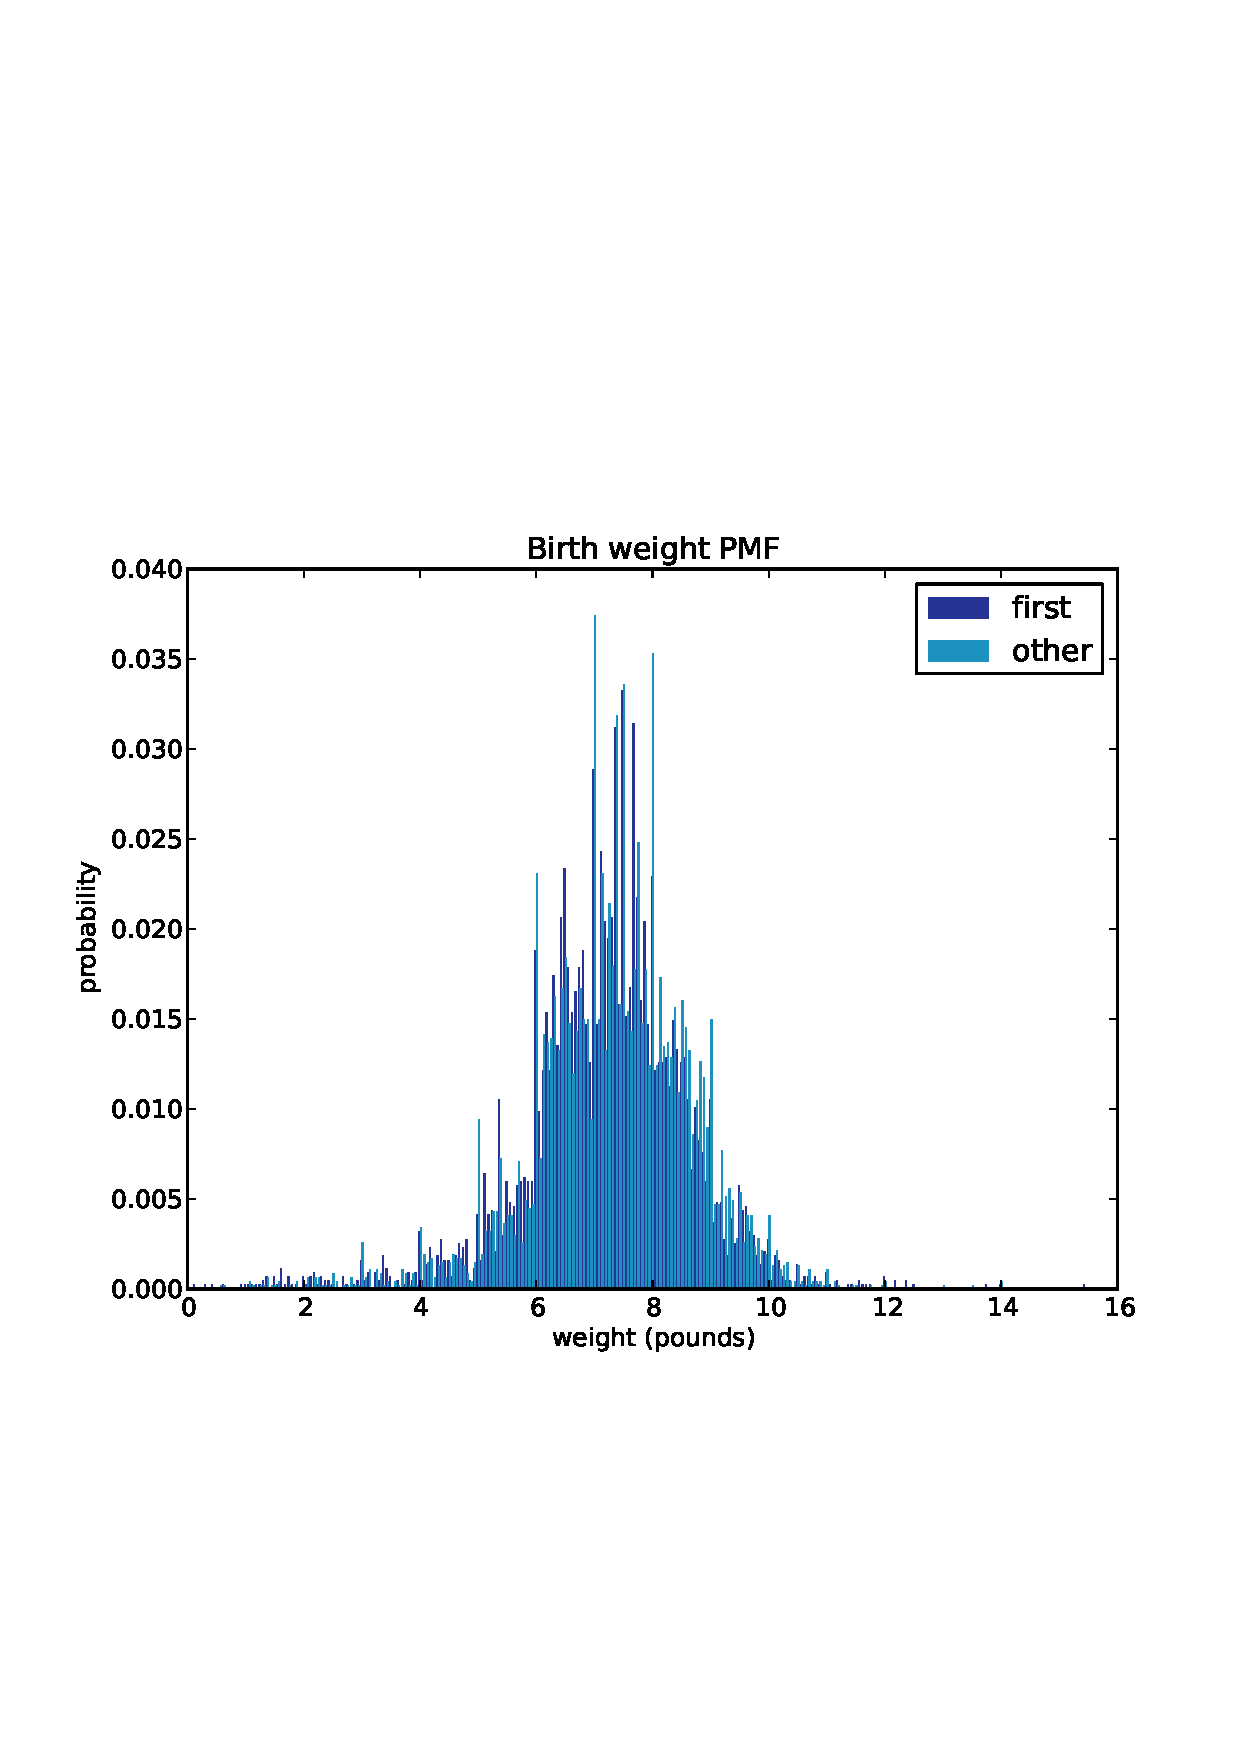
\includegraphics[height=2.5in]{figs/nsfg_birthwgt_pmf.pdf}}
\caption{출생체중 PMF. PMF의 한계를 그림이 보여주고 있다: 시작적으로 비교하기 어렵다.}
\label{nsfg_birthwgt_pmf}
\end{figure}

전반적으로 분포는 정규분포의 종모양을 닮았다.
평균 근처에 값이 많고 체중이 더 높거나 더 낮아지면 값이 작아진다.

하지만 그림을 이해하기는 어렵다. 뾰족한 것과 골자기가 많고, 두 집단 분포 사이에
명백한 차이도 보인다. 여럿중에서 어느 면이 유의미한지 분간하기는 쉽지 않다.
또한 전반적인 패턴을 보기도 어렵다; 예를 들어, 여러분이 보기에 어느 분포가 평균값이 더 높은가?
\index{통에 담기(binning)}

데이터를 구간(bin)에 담는 것으로 이러한 문제는 완화될 수 있다; 즉, 값 범위를 서로 겹쳐지지 않는 구간으로 
나누고 각 구간(bin)에 값 갯수를 계수한다. 구간에 담는 것(binning)은 유용하지만,
적정한 구간 크기를 잡는 것은 까다롭다. 잡음을 평활(smooth out)하기 위해서 충분히 큰 통을 잡는 것이 
또한 유용한 정보도 평활할 수도 있다.

이러한 문제를 회피하는 대안이 누적분포함수(cumulative
distribution function, CDF)로 이번 장 학습주제다. 하지만, CDF를 설명하기 전에 백분위수(percentile)를 먼저 설명해야 한다.
\index{CDF}


\section{백분위수 (Percentiles)}
\index{백분위 순위 (percentile rank)}

만약 전국 단위 표준시험을 치르게 되면, 원점수와 {\bf 백분위 순위(percentile rank)} 형태로 시험결과를 받아보게 된다. 이러한 맥락에서 백분위 순위는 시험 당사자보다 적은 점수를 얻는 사람들이 된다.
그래서 만약 ``백분위수 90번째''라면, 시험을 치른 90\% 사람보다 혹은 동등하다는 의미가 된다.

다음에 {\tt scores} 시퀀스 값에서 상대적으로 \verb"your_score" 값에 대한 백분위 순위를 계산하는 방법이 있다.

%
\begin{verbatim}
def PercentileRank(scores, your_score):
    count = 0
    for score in scores:
        if score <= your_score:
            count += 1

    percentile_rank = 100.0 * count / len(scores)
    return percentile_rank
\end{verbatim}

예제로 만약 시퀀스 점수가 55, 66, 77, 88, 99이고, 시험 점수로 88점을 받았다면, 
백분위 순위는 {\tt 100 * 4 / 5}, 80이 된다.

값이 주어진다면, 백분위 순위를 찾기는 쉽다; 반대 방향으로는 다소 더 어렵다.
만약 백분위 순위가 주어진 상태에서 해당하는 값을 찾고자 한다면, 한 선택지는 값을 정렬하고
원하는 값을 찾는 것이다.

%
\begin{verbatim}
def Percentile(scores, percentile_rank):
    scores.sort()
    for score in scores:
        if PercentileRank(scores, score) >= percentile_rank:
            return score
\end{verbatim}

계산 결과는 {\bf 백분위수(percentile)}가 된다. 
예를 들어, 50번째 백분위 수는 백분위 순위가 50 인 값이 된다. 
시험점수 분포에서 50번째 백분위 수는 77이다.
\index{백분위수 (percentile)}

{\tt Percentile} 구현코드가 그다지 효율적이지 않다.
더 나은 접근법은 백분위 순위를 사용해서 해당하는 백분위수 인덱스를 계산하는 것이다.

\begin{verbatim}
def Percentile2(scores, percentile_rank):
    scores.sort()
    index = percentile_rank * (len(scores)-1) // 100
    return scores[index]
\end{verbatim}

``백분위수 (percentile)''와 ``백분위 순위 (percentile rank)'' 차이가 혼동스러울 수 있고
항상 용어를 정확하게 구별하여 사용하지는 않는다. 요약하면,
{\tt PercentileRank} 함수는 값을 인자로 받아 값 집합에서 백분위 순위를 계산한다;
{\tt Percentile} 함수는 백분위 순위를 인자로 받아 해당하는 값을 계산한다. 
\index{백분위 순위 (percentile rank)}

\section{CDF}
\index{CDF}

이제 백분위수와 백분위 순위를 이해하고 있기 때문에, {\bf 누적분포함수(cumulative distribution function, CDF)}를 다룰 준비가 되었다. CDF는 값을 백분위 순위로 매핑하는 함수다.
\index{누적분포함수 (cumulative distribution function)}
\index{백분위 순위 (percentile rank)}

CDF는 $x$의 함수로 $x$는 분포에 나타나는 임의값이다.  
특정한 $x$ 값에 대해서 $\CDF(x)$를 평가하기 위해서, 
$x$와 동일하거나 작은 분포의 분수값을 계산한다.

시퀀스 {\tt sample}와 값 {\tt x}를 인자로 받는 함수로 어떤 느낌인지 다음에 코드가 있다.

%
\begin{verbatim}
def EvalCdf(sample, x):
    count = 0.0
    for value in sample:
        if value <= x:
            count += 1

    prob = count / len(sample)
    return prob
\end{verbatim}

함수가 거의 {\tt PercentileRank}과 동일하지만, 백분위 순위가 0--100인 반면에 결과값이 0--1 범위를 갖는 확률이라는 점이 차이가 있다.
\index{표본 (sample)}

예제로 표본값으로 {\tt [1, 2, 2, 3, 5]}을 수집했다고 가정하자. 다음에 CDF로부터 값이 몇개 있다.
%
\[ CDF(0) = 0 \]
%
\[ CDF(1) = 0.2\]
%
\[ CDF(2) = 0.6\]
%
\[ CDF(3) = 0.8\]
%
\[ CDF(4) = 0.8\]
%
\[ CDF(5) = 1\]
%

표본에 있는 값뿐만 아니라 $x$의 임의값에 대해서 CDF를 평가할 수 있다.
만약 $x$가 표본에 가장 작은 값보다 작다면, $\CDF(x)$는 0.
만약 $x$가 가장 큰 값보다 크다면, $\CDF(x)$는 1.

\begin{figure}
% cumulative.py
\centerline{\includegraphics[height=2.5in]{figs/cumulative_example_cdf.pdf}}
\caption{CDF 예제.}
\label{example_cdf}
\end{figure}

그림~\ref{example_cdf}이 CDF를 그래픽으로 표현한 것이다.
표본 CDF는 계단 함수다.
\index{계단 함수 (step function)}


\section{CDF 표현하기 (Representing CDFs)}
\index{Cdf}

{\tt thinkstats2}은 CDF를 표현하는 Cdf라는 클래스를 제공한다. Cdf 가 제공하는 기본 메쏘드는 다음과 같다.

\begin{itemize}

\item {\tt Prob(x)}: {\tt x} 값이 주어졌을 때, $p = \CDF(x)$ 확률값을 계산한다. 꺾쇠 연산자는 {\tt Prob}와 동일하다.
\index{꺾쇠 연산자 (bracket operator)}

\item {\tt Value(p)}: 확률 {\tt p}가 주어졌을 때, 
상응하는 값 {\tt x}를 계산한다; 즉, {\tt p}의 {\bf CDF 역함수(inverse CDF)}다.
\index{CDF 역함수 (inverse CDF)}
\index{CDF, 역함수(inverse)}

\end{itemize}

\begin{figure}
% cumulative.py
\centerline{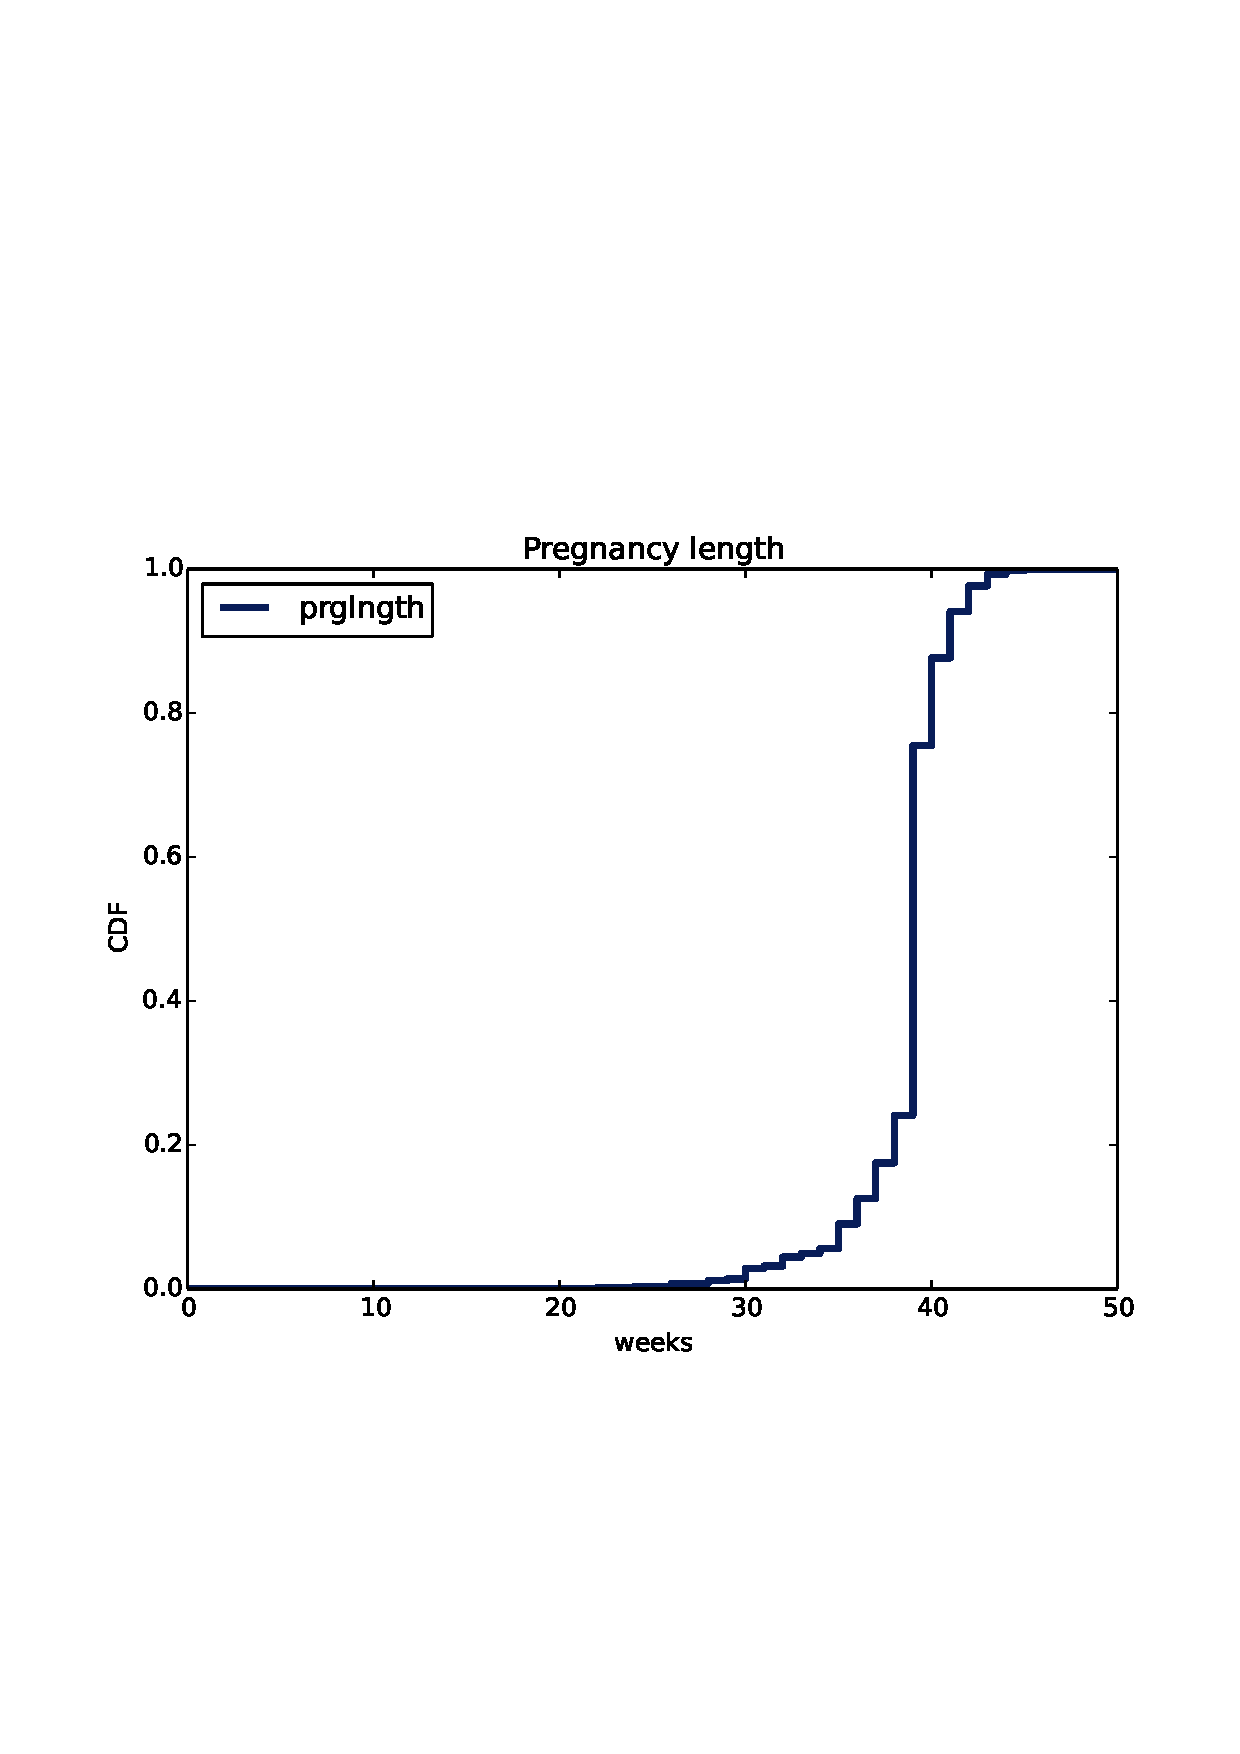
\includegraphics[height=2.5in]{figs/cumulative_prglngth_cdf.pdf}}
\caption{임신기간 CDF.}
\label{cumulative_prglngth_cdf}
\end{figure}

Cdf 생성자는 인자로 리스트, 판다스 시리즈, Hist, Pmf, 혹은 또다른 Cdf를 받을 수 있다. NSFG 데이터에서 임신 기간 분포에 대한 Cdf를 생성하는 코드가 다음에 있다. 

\index{NSFG}
\index{임신 기간 (pregnancy length)}

\begin{verbatim}
    live, firsts, others = first.MakeFrames()
    cdf = thinkstats2.Cdf(live.prglngth, label='prglngth')
\end{verbatim}


{\tt thinkplot}은 {\tt Cdf}라는 함수를 제공해서 Cdf를 선그래프를 그릴 수 있다.
\index{thinkplot}

\begin{verbatim}
    thinkplot.Cdf(cdf)
    thinkplot.Show(xlabel='weeks', ylabel='CDF')
\end{verbatim}



그림~\ref{cumulative_prglngth_cdf}에 결과가 있다.
CDF를 읽는 한가지 방법은 백분위수를 찾는 것이다.
예를 들어, 임신 기간 10\%는 36주차보다 더 짧고, 90\%는 41주차보다 더 짧은 것처럼 보인다. 또는 CDF를 통해서 분포 모양을 시각적으로 표현할 수도 있다. 흔한 값은 CDF에서 급격하거나 수직적 부분으로 나타난다; 이번 예제에서 39주차 모드(최빈값)가 명확히 보인다. 30주차 밑으로 값이 몇개 없어서 이 범위에 있는 CDF는 평평하다.
\index{CDF, 해석하기 (interpreting)}

CDF에 익숙해지는데 시간이 좀 필요하다. 하지만, 한번 익숙해지면, PMF보다 더 많은 정보를 좀더 명확하게 보여줄 것으로 생각된다.


\section{CDF 비교하기}
\label{birth_weights}
\index{가족 성장 국가 조사 (National Survey of Family Growth)}
\index{NSFG}
\index{출산 체중 (birth weight)}
\index{체중 (weight)!출산 (birth)}

CDF는 특히 분포를 비교하는데 유용하다.
예를 들어, 첫째 아이와 첫째 아이가 아닌 아이에 대한 출산 체중 CDF를 플롯으로 그리는 코드가 다음에 있다.
\index{thinkplot}
\index{분포 (distributions), 비교하기 (comparing)}

\begin{verbatim}
    first_cdf = thinkstats2.Cdf(firsts.totalwgt_lb, label='first')
    other_cdf = thinkstats2.Cdf(others.totalwgt_lb, label='other')

    thinkplot.PrePlot(2)
    thinkplot.Cdfs([first_cdf, other_cdf])
    thinkplot.Show(xlabel='weight (pounds)', ylabel='CDF')
\end{verbatim}

\begin{figure}
% cumulative.py
\centerline{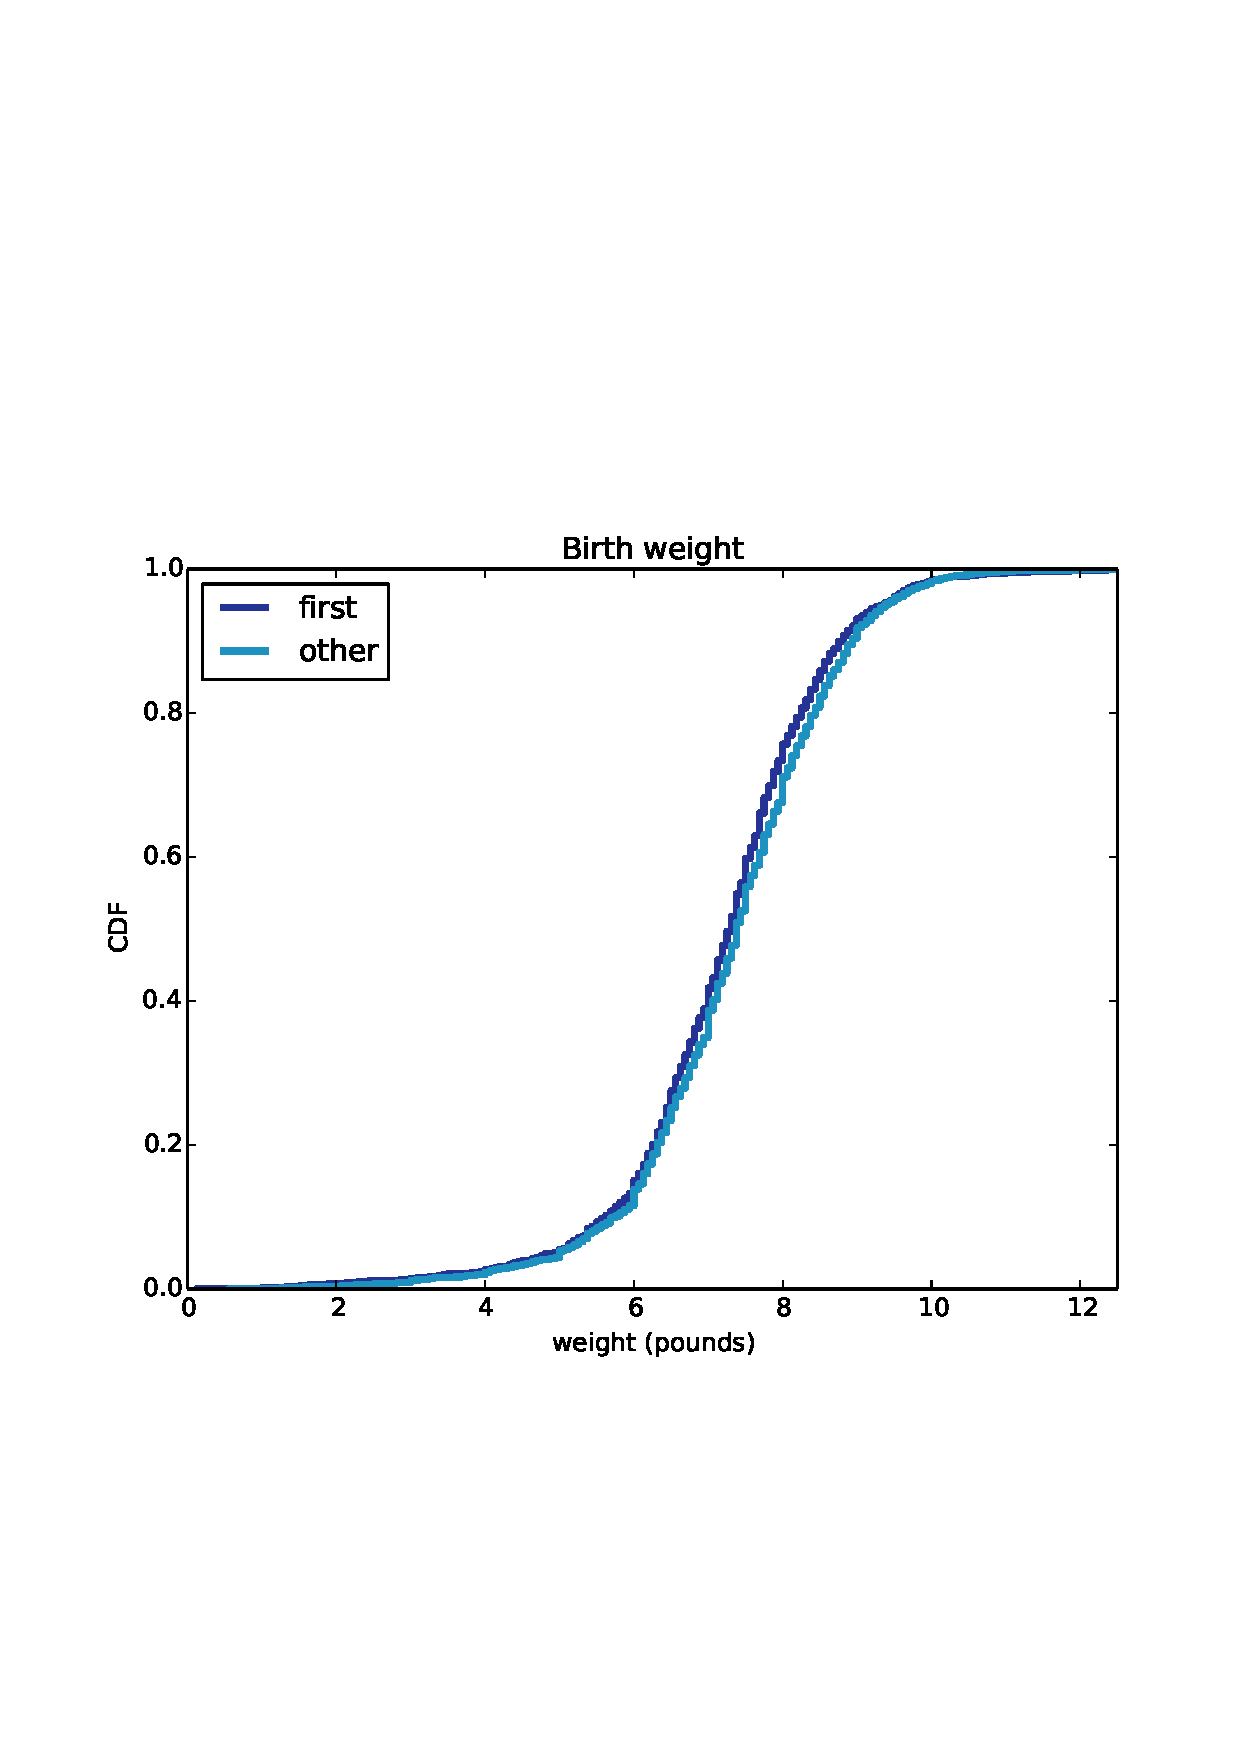
\includegraphics[height=2.5in]{figs/cumulative_birthwgt_cdf.pdf}}
\caption{첫째 아기와 첫째가 아닌 아기에 대한 출산체중 CDF.}
\label{cumulative_birthwgt_cdf}
\end{figure}

그림~\ref{cumulative_birthwgt_cdf}에 결과가 있다.
그림~\ref{nsfg_birthwgt_pmf}와 비교하여, 좀더 명확하게 분포 모양과 분포간의 차이를 그림에서 보여준다.
첫째 아이 체중이 평균 이상에서 조금더 커다란 불일치성을 보이고, 분포 전반에 걸쳐 다소 가볍다는 것을 볼 수 있다.

\index{모양 (shape)}

\section{백분위수 기반 통계량 (Percentile-based statistics)}
\index{요약 통계 (summary statistic)}
\index{사분위수 범위 (interquartile range)}
\index{분위수 (quartile)}
\index{백분위수 (percentile)}
\index{중위수 (median)}
\index{중심 경향성 (central tendency)}
\index{퍼짐 (spread)}

CDF를 계산하게 되면, 백분위수와 백분위 순위를 계산하기는 쉽다.
Cdf 클래스가 두가지 메쏘드를 제공한다.
\index{Cdf}
\index{백분위 순위 (percentile rank)}

\begin{itemize}

\item {\tt PercentileRank(x)}: {\tt x}가 주어지면, $100 \cdot \CDF(x)$ 백분위 순위를 계산한다.

\item {\tt Percentile(p)}: 백분위 순위 {\tt rank}가 주어지면,
해당하는 값 {\tt x}를 계산한다. {\tt Value(p/100)}과 동등하다.

\end{itemize}

{\tt 백분위수 (Percentile)}는 백분위수 기반 요양 통계량을 계산하는데 사용될 수 있다. 예를 들어 50번째 백분위수는 {\bf 중위수 (median)}로 알려진 분포를 반으로 나누는 값이다. 평균과 마찬가지로 중위수는 분포의 중심경향성을 측정하는 측도다.

사실, 각기 다른 특성을 가진 ``중위수(median)''에 대한 정의가 몇개 있다. 하지만, {\tt Percentile(50)}가 단순하고 계산하기 효율적이다.

또 다른 백분위수 기반 통계량이 {\bf 사분위수 범위 (interquartile range, IQR}로 분포의 퍼짐을 측정하는 측도다.
IQR는 75번째와 25번째 백분위수 간의 차이다.

좀더 일반적으로, 백분위수는 종종 분포 모양을 요약하는데 쓰여진다.
예를 들어, 수입 분포는 종종 ``분위수 (quintiles)''로 보고된다; 즉, 20번째, 40번째, 60번째, 80번째 백분위수로 쪼개진다.
다른 분포는 10개 ``십분위(deciles)''으로 나눠진다.
이와 같이 CDF에서 동일간격으로 표현되는 통계량을 {\bf 분위수(quantiles)}라고 한다. 좀더 자세한 정보는 다음 웹사이트를 참고 바란다. \url{https://en.wikipedia.org/wiki/Quantile}.
\index{분위수 (quantile)}
\index{오분위수 (quintile)}
\index{십분위수 (decile)}


\section{난수 (Random numbers)}
\label{random}
\index{난수 (random number)}

정상 출산 모집단에서 임의 표본을 추출하고, 출생 체중 백분위 순위를 찾아낸다고 가정하자. 이제 백분위 순위 CDF를 계산한다고 가정하자.
분포가 어떨 것으로 생각하는가?

\index{백분위 순위 (percentile rank)}
\index{출생 체중 (birth weight)}
\index{체중 (weight)!출생 (birth)}

다음에 어떻게 계산하는지 코드가 있다. 첫째로 출생 체중 Cdf를 생성한다.
\index{Cdf}

\begin{verbatim}
    weights = live.totalwgt_lb
    cdf = thinkstats2.Cdf(weights, label='totalwgt_lb')
\end{verbatim}

그리고 나서, 표본을 생성하고, 표본에 있는 각 값에 대한 백분위 순위를 계산한다.

\begin{verbatim}
    sample = np.random.choice(weights, 100, replace=True)
    ranks = [cdf.PercentileRank(x) for x in sample]
\end{verbatim}

{\tt sample}은 100개 출생 체중 임의 표본이며 복원 추출하였다;
즉, 동일한 값이 한번이상 추출될 수 있다. 
{\tt ranks}는 백분위 순위 리스트다.
\index{복원 (replacement)}

마지막으로 백분위 순위 Cdf를 만들고 플롯으로 그린다.

\index{thinkplot}

\begin{verbatim}
    rank_cdf = thinkstats2.Cdf(ranks)
    thinkplot.Cdf(rank_cdf)
    thinkplot.Show(xlabel='percentile rank', ylabel='CDF')
\end{verbatim}

\begin{figure}
% cumulative.py
\centerline{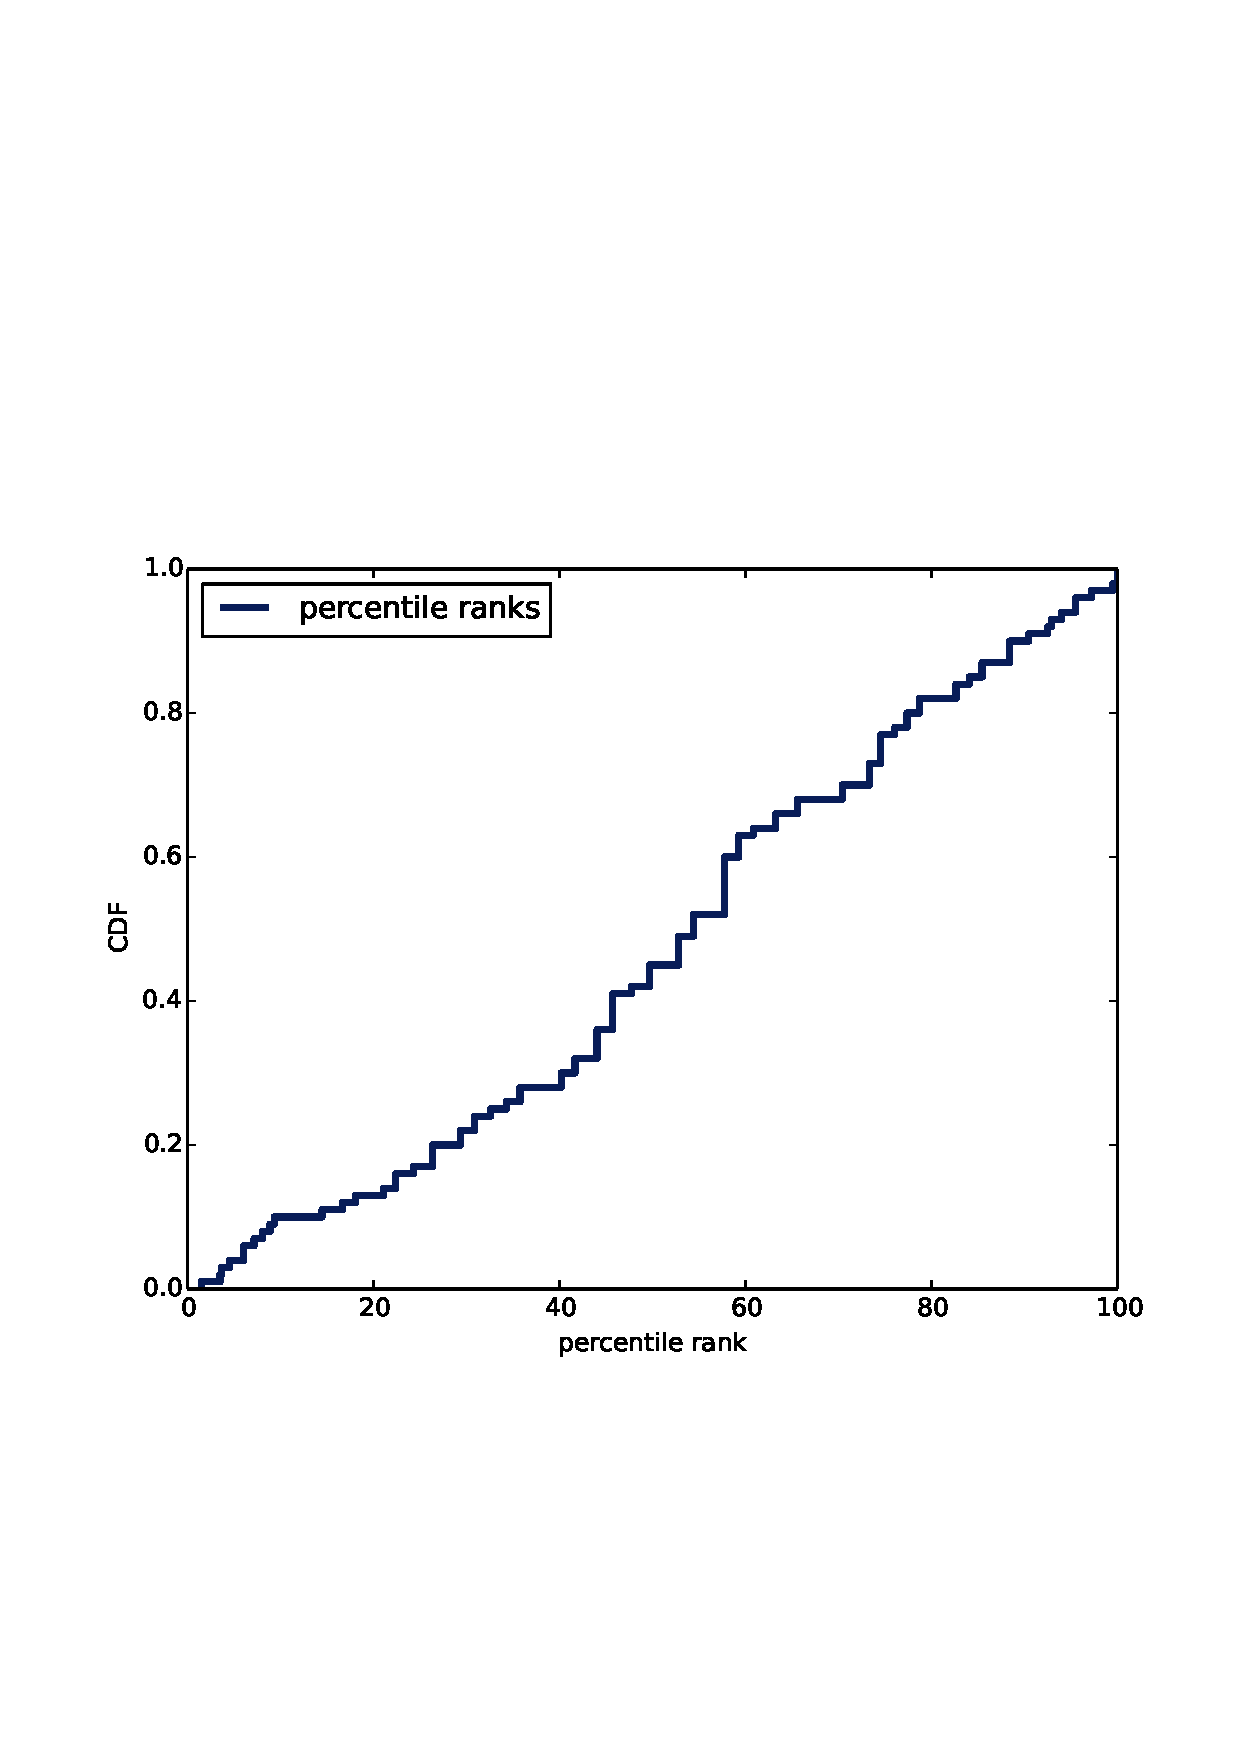
\includegraphics[height=2.5in]{figs/cumulative_random.pdf}}
\caption{출생체중 임의 표본에 대한 백분위 순위 CDF.}
\label{cumulative_random}
\end{figure}

그림~\ref{cumulative_random}이 결과를 보여준다.
CDF가 근사적으로 직선이다. 분포가 균등하다라는 의미다. 

결과가 명확하지 않을 수도 있지만, CDF가 정의된 방식의 결과다.
그림이 보여주는 정보는 표본의 10\%가 10번째 백분위수 보다 밑에 있고,
표본의 20\%가 20번째 백분위수 보다 밑에 있고 등등, 정확히 예측했던 것이다.

그래서, CDF 모양에 관계없이, 백분위 순위 분포는 균등하다. 
이 속성이 유용한데, 이유는 주어진 CDF에서 난수를 생성하는데 있어서 간단하면서도 효율적인 알고리즘 설계하는 기초가 되기 때문이다; 다음에 난수를 생성하는 방법이 있다.

\index{역 CDF 알고리즘 (inverse CDF algorithm)}
\index{난수 (random number)}

\begin{itemize}

\item 0--100 범우에서 균등하게 백분위 순위를 고른다.

\item {\tt Cdf.Percentile}를 사용해서 선택한 백분위 순위에 상응하는 값을 분포에서 찾는다.
\index{Cdf}

\end{itemize}

Cdf는 상기 알고리즘을 구현한 것으로 {\tt Random}이 함수명이다.

\begin{verbatim}
# class Cdf:
    def Random(self):
        return self.Percentile(random.uniform(0, 100))
\end{verbatim}

Cdf는 {\tt Sample} 메쏘드를 제공하는데 정수 {\tt n}을
인자로 받아 Cdf에서 임의로 추출한 {\tt n}개 리스트를 반환한다.


\section{백분위 순위 비교하기}

백분위 순위는 다른 집단에 대해서 측정값을 비교하는데 유용하다.
예를 들어, 달리기 경주에서 참가자는 대체로 나이와 성별로 무리를 만든다.
다른 연령 집단에 있는 사람을 비교하는데 경주시간을 백분위 순위로 변환할 수 있다.

\index{백분위 순위 (percentile rank)}

몇년전에 매사추세츠(Massachusetts)주에서 제임스 조이스(James Joyce) 10킬로 마라톤을 뛰었다;
42분 44초로 주파해서 1633명중에서 97번째로 완주했다. 참가자 1633명 중 1537명 참가자보다 빨리 도착해서 
저자의 최종 백분위 순위는 94\%다.  
\index{제임스 조이스 마라톤 (James Joyce Ramble} 
\index{경주 시간 (race time)}


좀더 일반적으로, 위치와 필드 크기 정보가 주어진다면, 백분위 순위를 계산할 수 있다.
\index{필드 크기 (field size)}

\begin{verbatim}
def PositionToPercentile(position, field_size):
    beat = field_size - position + 1
    percentile = 100.0 * beat / field_size
    return percentile
\end{verbatim}

``40에서 49세 남성'', M4049로 표기된 저자가 속한 연령집단, 256명 중에서 26번째로 완주했다.
그래서, 저자가 속한 연령집단에서 백분위 순위는 90\%가 된다.
\index{연령 집단 (age group)}

10년정도 더 마라톤을 뛴다면 (그리고 계속해서 뛰고 싶다.), M5059 그룹에 있을 것이다.
저자가 속한 집단에서 동일한 백분위수를 유지한다고 가정한다면, 완주하는데 얼마나 더 시간이 필요할까?

M4049 집단에 있는 저자의 백분위 순위를 M5059 집단에 위치로 전환하면 상기 질문에 대답할 수 있다.
다음에 프로그램 코드가 있다.

\begin{verbatim}
def PercentileToPosition(percentile, field_size):
    beat = percentile * field_size / 100.0
    position = field_size - beat + 1
    return position
\end{verbatim}

M5059 집단에 171 명이 있어서 동일한 백분위 순위를 유지하려면 17번째와 18번째 사이에서 완주해야 한다.
M5059에서 17번째 마라토너가 46:05로 완주해서, 40대 동일한 백분위 순위를 유지하는데 
46:05 시간이 완주 목표시간이 된다.


\section{Exercises}

아래 연습문제에 대해서, \verb"chap04ex.ipynb" 파일로 시작할 수 있다.
저자 해답은 \verb"chap04soln.ipynb" 파일에 나와 있다.

\begin{exercise}
여러분 출생당시 몸무게가 얼마나 되나요? 
만약 몸무게를 알지 못한다면, 엄마나 혹은 아는 누군가에 전화해서 알아보세요.
(모든 정상출생) NSFG 데이터를 사용해서, 출생 체중의 분포를 계산하고,
이를 사용해서 여러분의 백분위수를 알아내세요.
만약 첫째라면, 첫번째 아이에 대해서 분포의 백분위수를 알아내세요.
첫째가 아니라면, 첫째가 아닌 아이에 대한 분포를 사용하세요.
만약 백분위수 90번째 혹은 그 이상이라면, 엄마에게 다시 전화해서 사과하세요.

\index{출생 체중}
\index{체중!출생}

\end{exercise}

\begin{exercise}
{\tt random.random}에서 생성된 숫자는 0과 1 사이에서 균등하게 나올 것으로 간주된다;
즉, 이 범위 모든 값은 동일한 확률을 가져야만 된다.

{\tt random.random}에서 난수 1000개를 생성하고 PMF와 CDF를 도식화하시오.
이 분포는 균등분포인가?

\index{균등 분포}
\index{분포!균등}
\index{난수}

\end{exercise}


\section{용어사전}

\begin{itemize}

\item 백분위 순위 (percentile rank): 
분포에서 주어진 값과 동일하거나 적은 값의 퍼센티지.
\index{백분위 순위 (percentile rank)}

\item 백분위수 (percentile): 주어진 백분위 순위와 연관된 값.
\index{백분위수 (percentile)}

\item 누적분포함수 (cumulative distribution function, CDF): 
값에서 누적확률값으로 매핑하는 함수. $\CDF(x)$는 $x$와 동일하거나 작은 표본비율이다. 
\index{CDF}
\index{누적 확률 (cumulative probability)}

\item 역 CDF (inverse CDF):
누적 확률($p$)에서 해당값으로 매핑하는 함수.
\index{역 CDF (inverse CDF)}
\index{CDF, 역 (inverse)}

\item 중위수 (median): 
종종 중심경향성 측도로 사용되는 50번째 백분위수.
\index{중위수 (median)}

\item 사분위 범위 (interquartile range): 
퍼짐의 측도로 사용되는 75번째와 25번째 백분위수 간 차이.
\index{사분위 범위 (interquartile range)}

\item 분위수 (quantile): 
동일 간격 백분위 순위에 상응하는 스퀀스 값; 예를 들어, 
분포 사분위수는 25번째, 50번째, 75번째 백분위수가 된다.
\index{분위수 (quantile)}

\item 복원 (replacement): 
표본추출 과정의 속성. ``복원추출 (With replacement)''는 동일한 값이 한번이상 추출될 수 있다는 의미다;
``비복원추출 (Without replacement)''는 값이 한번 추출될면, 모집단에서 제거된다는 의미가 된다.
\index{복원 (replacement)}

\end{itemize}


\chapter{분포 모형화 (Modeling distributions)}
\label{modeling}

지금까지 사용한 분포는 {\bf 경험적 분포 (empirical distributions)}라고 부른다.
이유는 필연적으로 유한 표본인 경험적 관측치에 기반하고 있기 때문이다.

\index{해석 분포 (analytic distribution)}
\index{분포 (distribution)!해석 (analytic)}
\index{경험적 분포 (empirical distribution)}
\index{분포 (distribution)!경험 (empirical)}

수학 함수인 CDF로 특징 지어지는 {\bf 해석 분포 (analytic distribution)}가 대안이 된다.
해석 분포가 경험적 분포를 모형화하는데 사용될 수 있다.
이러한 맥락에서 {\bf 모형(model)}은 불필요한 부분을 덜어낸 단순화가 된다.
이번 장에서 자주 사용되는 분포를 제시하고 이를 사용하여 다양한 출처를 가진 
데이터를 모형화한다.

\index{모형 (model)}

이번 장에서 사용되는 코드는 {\tt analytic.py}에 있다.
코드를 다운로드하고 작업하는 것에 대한 정보는 ~\ref{code}을 참조한다.


\section{지수분포 (exponential distribution)}
\label{exponential}
\index{지수분포 (exponential distribution)}
\index{분포 (distribution)!지수 (exponential)}

\begin{figure}
% analytic.py
\centerline{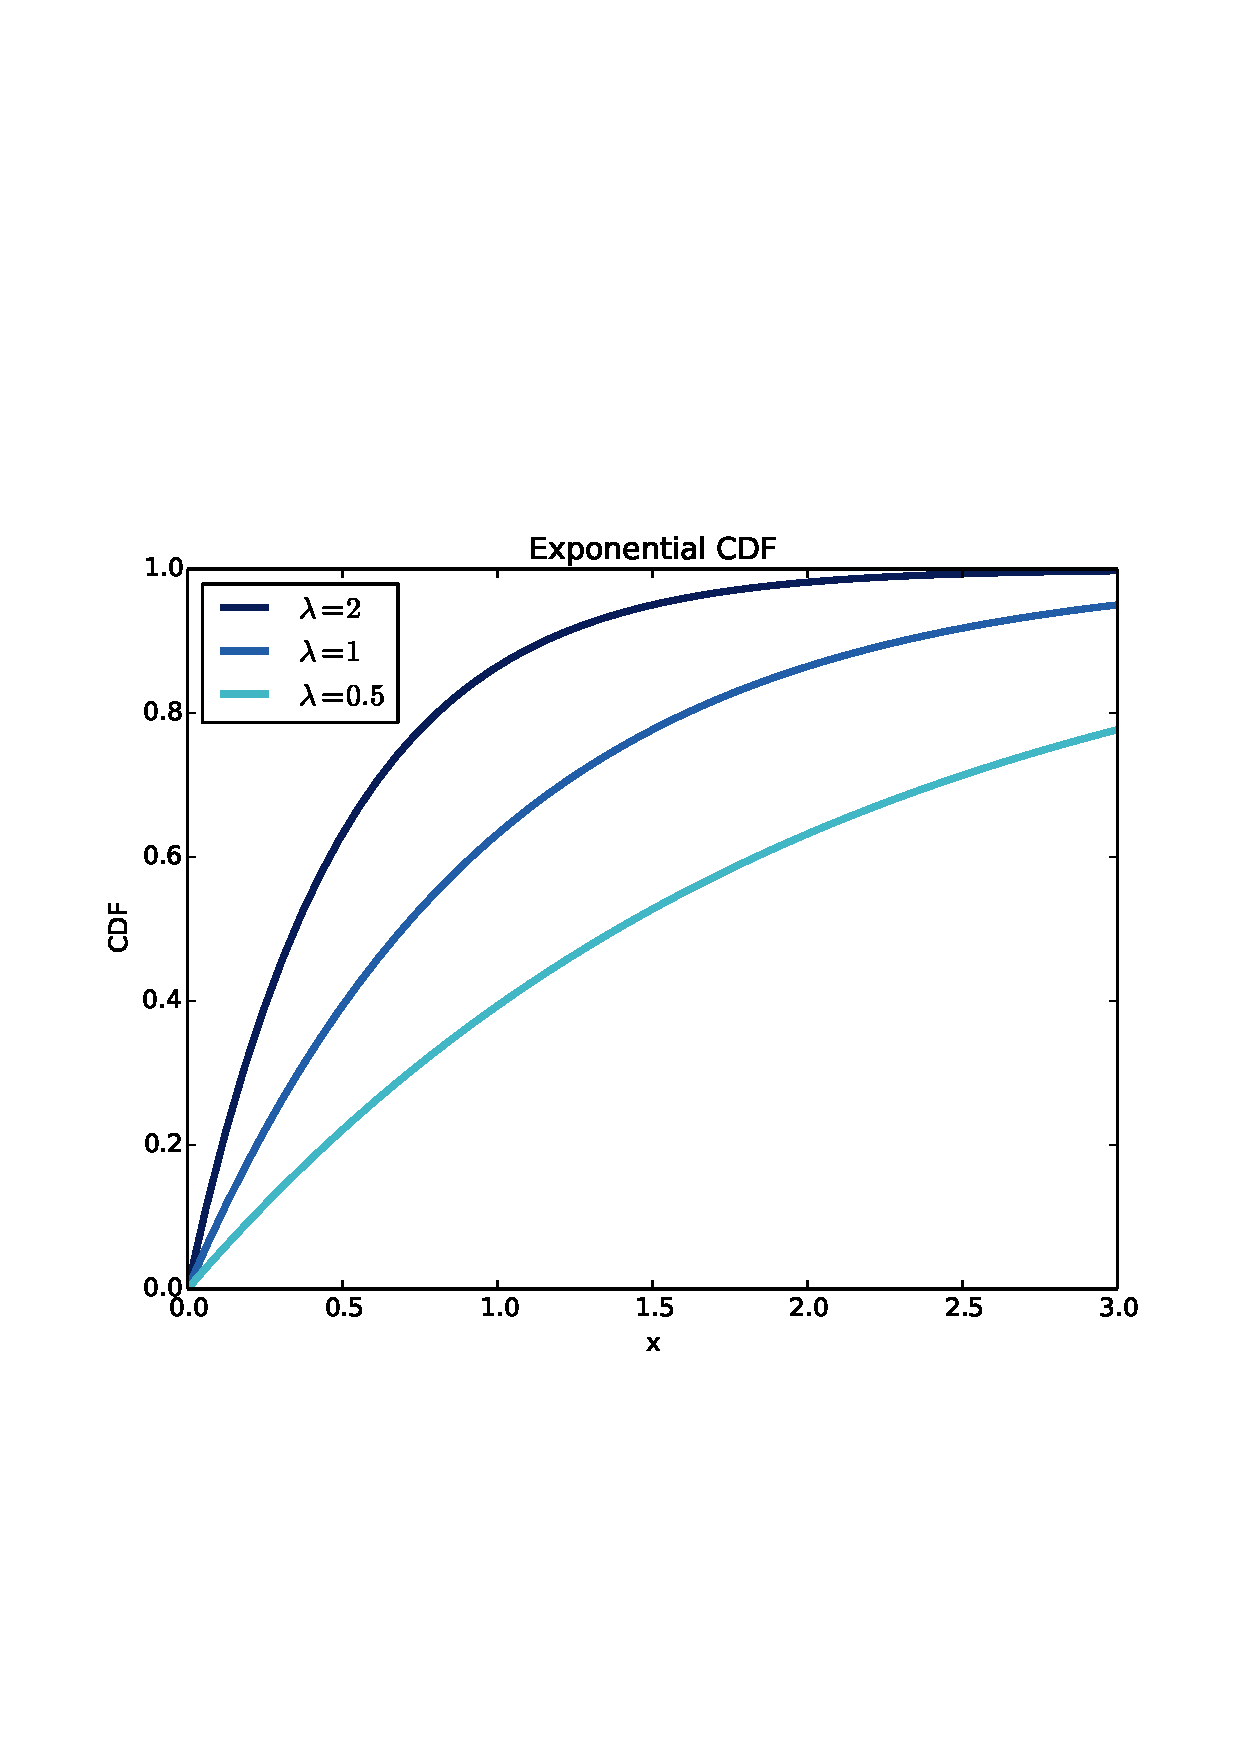
\includegraphics[height=2.5in]{figs/analytic_expo_cdf.pdf}}
\caption{다양한 모수를 갖는 지수분포 CDF.}
\label{analytic_expo_cdf}
\end{figure}

{\bf 지수 분포 (exponential distribution)}로 시작하는데 이유는 상대적으로 단순하기 때문이다.
지수분포 CDF는 다음과 같다.
%
\[ \CDF(x) = 1 - e^{-\lambda x} \]
%

모수 $\lambda$가 분포 형상(shape)을 결정한다. 
그림~\ref{analytic_expo_cdf}에서 $\lambda = $ 0.5, 1, 2 값을 가진
CDF가 대략 모양이 어떤지 볼 수 있다.
\index{모수 (parameter)}

현실 세계에서 일련의 사건을 보고, 사건 간에 시간({\bf 도착간격 시간, interarrival times})을 측정할 때 지수분포가 등장한다.
만약 사건이 언제든지 균등하게 발생할 것 같다면 도착간격 시간 분포는 지수분포같은 경향이 있다.
\index{도착간격 시간 (interarrival time)}

일례로, 출생간 발생시간을 살펴보자. 1997년 12월 18일 호주 브리즈번
\footnote{예제에 나오는 자료와 정보는 저널 논문에 기반한다. Dunn, ``A Simple Dataset for Demonstrating Common Distributions,'' Journal of Statistics Education v.7, n.3 (1999)}
에서 44명 신생아가 출생했다. 모든 44명 신생아 출생 시간이 지역신문에 출간되었다;
전체 데이터셋은 {\tt ThinkStats2} 저장소 {\tt babyboom.dat} 파일에 담겨있다.
\index{출생 시간 (birth time)}
\index{호주 (Australia)} 
\index{브리즈번 (Brisbane)}

\begin{verbatim}
    df = ReadBabyBoom()
    diffs = df.minutes.diff()
    cdf = thinkstats2.Cdf(diffs, label='actual')

    thinkplot.Cdf(cdf)
    thinkplot.Show(xlabel='minutes', ylabel='CDF')
\end{verbatim}

{\tt ReadBabyBoom} 함수가 데이터 파일을 읽어들이고 {\tt time}, {\tt sex}, \verb"weight_g", {\tt minutes}
칼럼으로 구성된 데이터프레임을 반환한다.
여기서 {\tt minutes}가 자정 이후 출생시간을 분으로 변환한 시간정보를 담고 있다.
\index{데이터프레임 (DataFrame)}
\index{thinkplot}

\begin{figure}
% analytic.py
\centerline{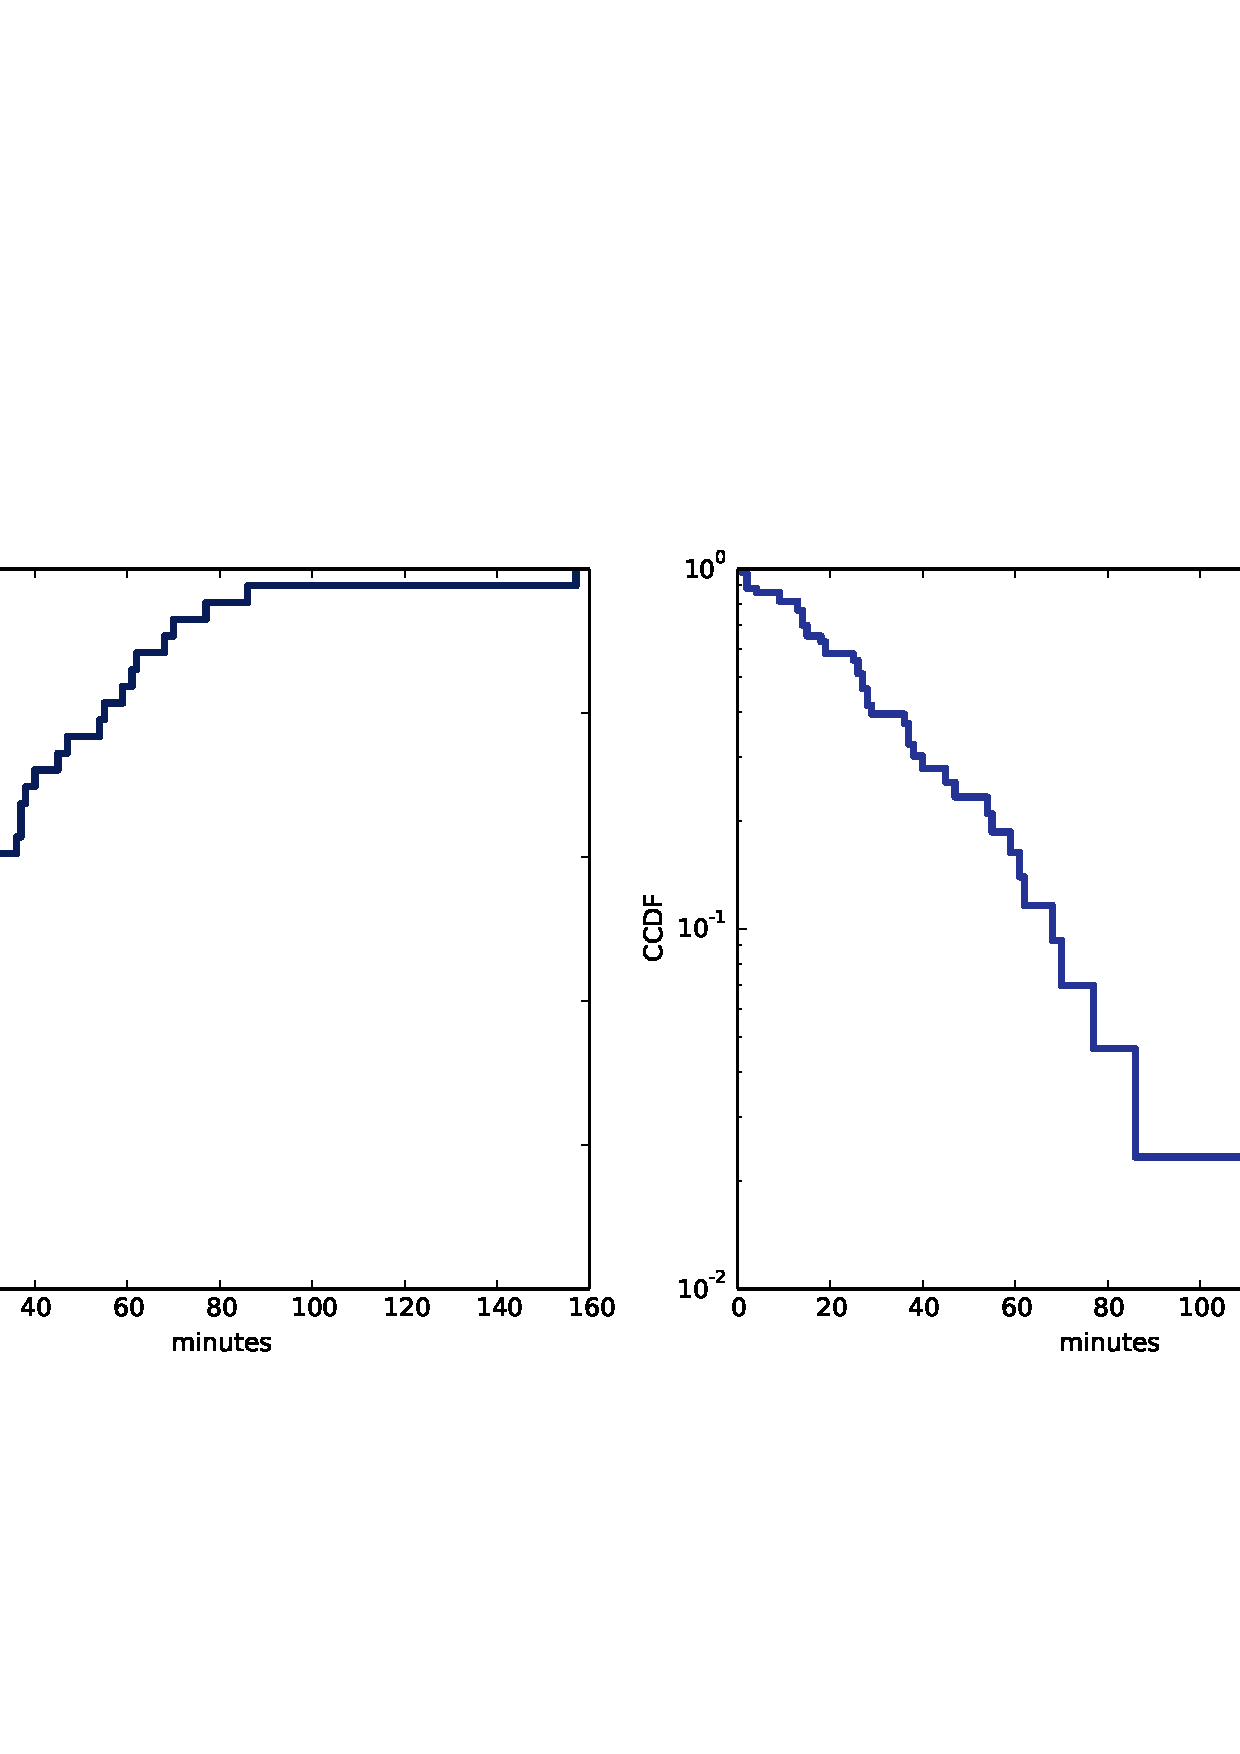
\includegraphics[height=2.5in]{figs/analytic_interarrivals.pdf}}
\caption{도착간격시간 CDF (좌측), log-y 척도로 된 CCDF (우측).}
\label{analytic_interarrival_cdf}
\end{figure}

%\begin{figure}
% analytic.py
%%\centerline{\includegraphics[height=2.5in]{figs/analytic_interarrivals_logy.pdf}}
%\caption{CCDF of interarrival times.}
%\label{analytic_interarrival_ccdf}
%\end{figure}

{\tt diffs}는 연속되는 출생시간 사이 차이가 되고 
{\tt cdf}는 출생간격 시간 분포가 된다.
그림~\ref{analytic_interarrival_cdf} (왼편)이 CDF를 나타낸다.
전형적인 지수분포 형상을 지닌 처럼 보이지만, 어떻게 분간할 수 있을까?

한 방법은 {\bf 보완 CDF (complementary CDF)}를 플롯으로 그리는 것이다.
보완 CDF는 log-y 척도로 $1 - \CDF(x)$이다.
지수분포 데이터에 대해서는 결과가 직선이다. 왜 그런지 살펴보자.

\index{보완 CDF (complementary CDF)} 
\index{CDF!보완 (complementary)} 
\index{CCDF}

독자가 생각하기에 지수분포를 따르는 데이터셋을 보완 CDF(CCDF) 플롯으로 그리면, 
다음과 같은 함수가 나올 것으로 기대한다.
%
\[ y \approx e^{-\lambda x} \]
%
양변에 로그를 취하면 다음과 같다.
%
\[ \log y \approx -\lambda x\]
%
그래서, log-y 척도로 CCDF는 기울기 $-\lambda$인 직선이 된다.
다음에 플롯을 생성하는 방법이 있다.
\index{로그 척도 (logarithmic scale)}
\index{보완 CDF (complementary CDF)}
\index{CDF!보완 (complementary)}
\index{CCDF}

\begin{verbatim}
    thinkplot.Cdf(cdf, complement=True)
    thinkplot.Show(xlabel='minutes',
                   ylabel='CCDF',
                   yscale='log')
\end{verbatim}

{\tt complement=True} 인자가 있어서, {\tt thinkplot.Cdf}이 플롯을 그리기 전에
보완 CDF를 계산한다. 그리고 {\tt yscale='log'}를 통해서  
{\tt thinkplot.Show}가 로그 척도로 {\tt y}축을 고정한다.
\index{thinkplot}
\index{Cdf}

그림~\ref{analytic_interarrival_cdf} (오른편)에 결과가 있다.
정확하게 직선이 아니다. 이 데이터에 대해서 완벽한 모델로 지수 분포가 아니라는 것이 표시된다.
기본 가정---출생이 아무 때고 균등하게 발생---이 정확하게 사실이 아닐 것이다.
그럼에도 불구하고 지수분포로 이 데이터셋을 모형화하는 것이 합리적일 것이다.
이와 같은 단순화로 단 하나의 모수로 분포를 요약할 수 있다.
\index{모형 (model)}

모수 $\lambda$가 율(rate)로 해석될 수 있다; 즉, 평균적으로 단위 시간에 
발생하는 사건 수. 예제에서 44명의 신생아가 24시간내에 태어난다.
그래서 율값이 분당 $\lambda = 0.0306$이 된다.
지수분포 평균은 $1/\lambda$ 으로 신생아 간에 출생 평균 시간은 32.7분이 된다.

\section{정규 분포 (normal distribution)}
\label{normal}

가우스 분포(Gaussian distribution)라고도 불리는 
{\bf 정규 분포 (normal distribution)}가 흔히 사용되는데 이유는 많은 현상을 기술하고 
최소한 근사적으로도 기술할 수 있기 때문이다.
\ref{CLT} 절에서 다루게 되는데 이와 같은 보편성에는 이유가 있다.
\index{CDF}
\index{모수 (parameter)}
\index{평균 (mean)}
\index{표준편차 (standard deviation)}
\index{정규 분포 (normal distribution)}
\index{분포 (distribution)!정규 (normal)}
\index{가우스 분포 (Gaussian distribution)}
\index{분포 (distribution)!가우스 (Gaussian)}

%
\[ \CDF(z) = \frac{1}{\sqrt{2 \pi}} \int_{-\infty}^z e^{-t^2/2} dt \]
%

\begin{figure}
% analytic.py
\centerline{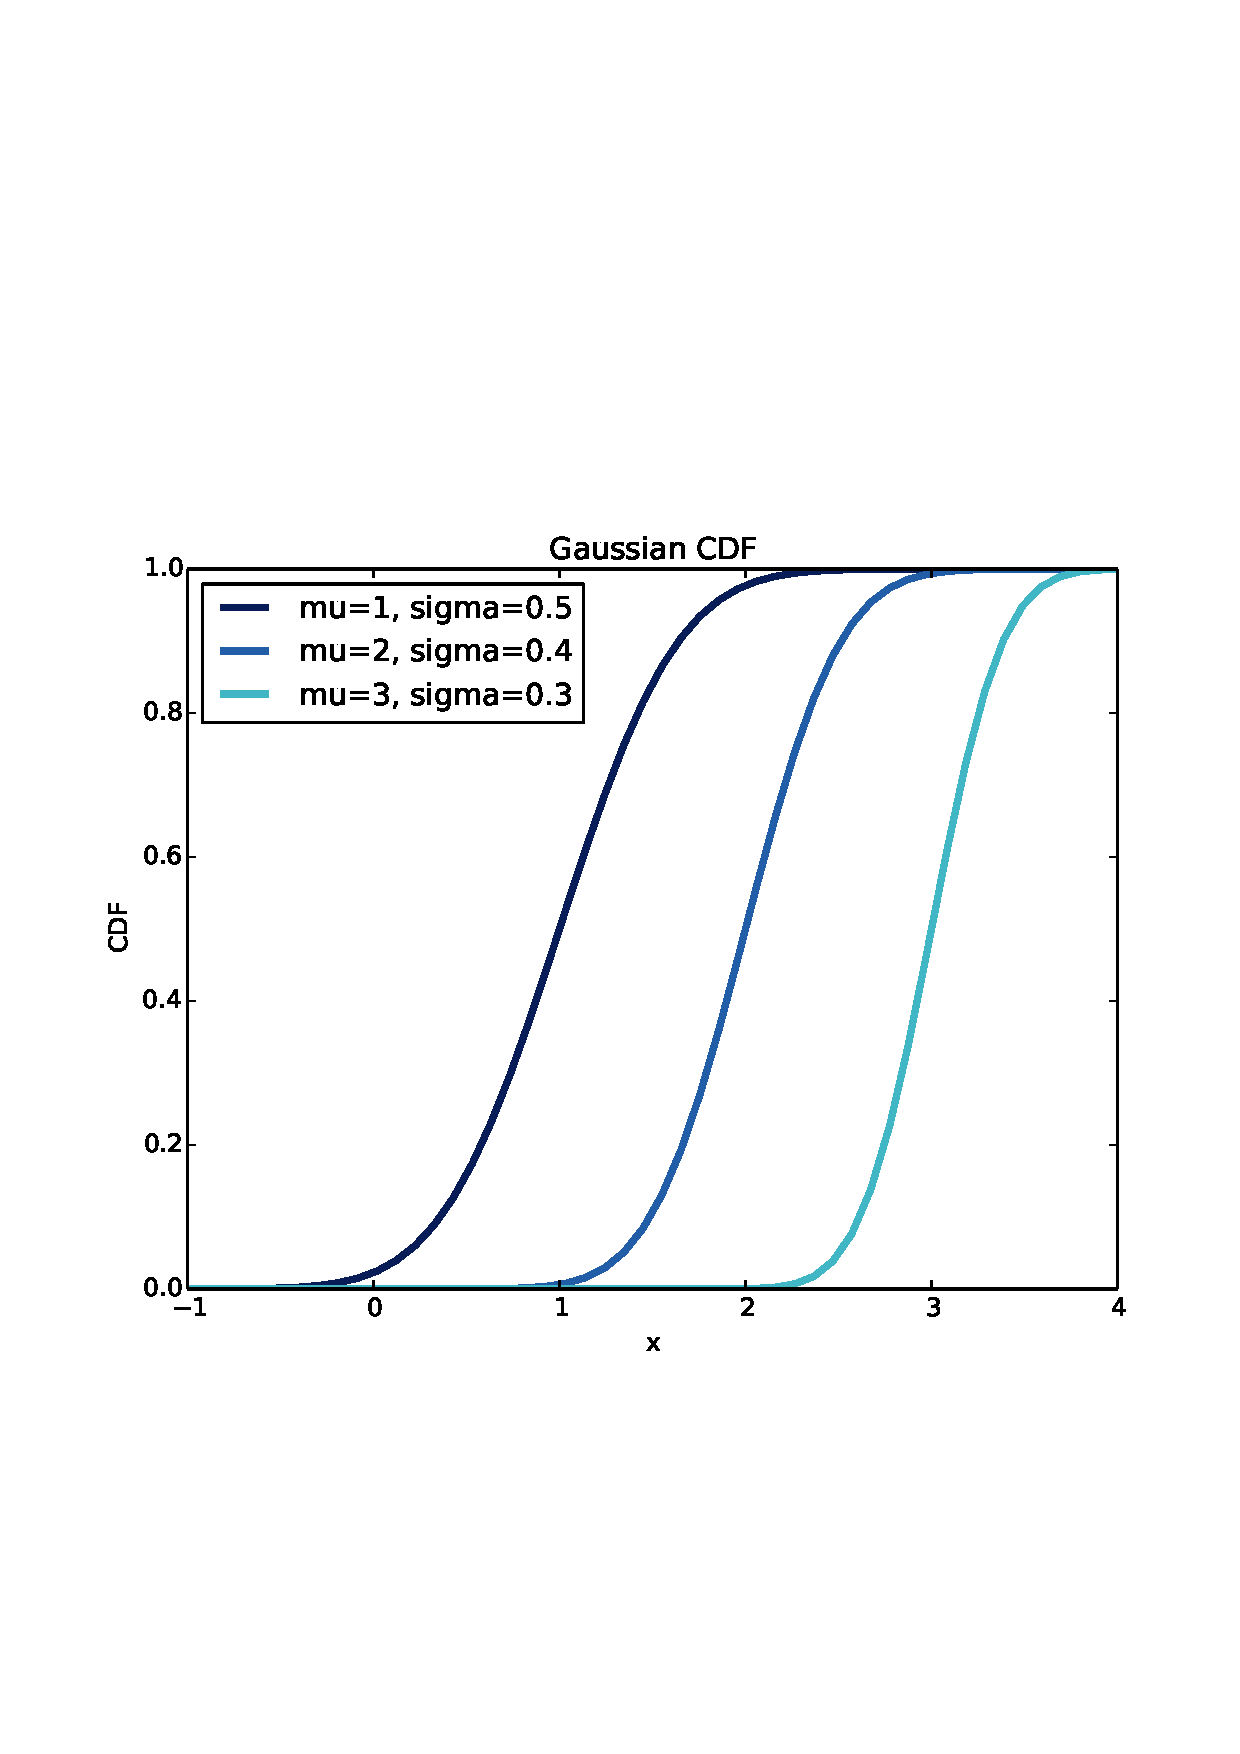
\includegraphics[height=2.5in]{figs/analytic_gaussian_cdf.pdf}}
\caption{모수 범위에 따른 정규분포 CDF.}
\label{analytic_gaussian_cdf}
\end{figure}

정규 분포는 모수 두개로 특성화된다: 평균 $\mu$, 표준편차 $\sigma$.
모수 $\mu=0$과 $\sigma=1$을 갖는 정규분포를 {\bf 표준 정규 분포 (standard normal
 distribution)}라고 한다.
정규분포 CDF는 닫힌 형식 해법(closed form solution)을 갖지 않는 적분으로 정의된다.
하지만, 효율적으로 계산하는 알고리즘이 있다.
알고리즘 중 하나가 SciPy을 통해 제공된다: {\tt scipy.stats.norm}이
정규분포를 표현하는 객체다. 표준 정규분포 CDF를 계산하는 {\tt cdf} 메쏘드를 제공한다.

\index{SciPy}
\index{닫힌 형식 (closed form)}

\begin{verbatim}
>>> import scipy.stats
>>> scipy.stats.norm.cdf(0)
0.5
\end{verbatim}

결과값은 맞다: 표준 정규분포 중위수는 0 (평균과 같다)이고, 값의 절반이 중위수 아래 위치한다.
그래서 $\CDF(0)$은 0.5 이다.

{\tt norm.cdf}은 옵션 모수를 받는다: {\tt loc}가
평균을 특정하고, {\tt scale}는 표준편차를 특정한다.


{\tt thinkstats2}는 상기 함수를 좀더 사용하기 쉽게 한다.
{\tt EvalNormalCdf} 메쏘드는 {\tt mu}과 {\tt sigma}을 인자로 받아 
{\tt x}에 CDF를 계산한다.

\index{정규 분포 (normal distribution)}

\begin{verbatim}
def EvalNormalCdf(x, mu=0, sigma=1):
    return scipy.stats.norm.cdf(x, loc=mu, scale=sigma)
\end{verbatim}

그림~\ref{analytic_gaussian_cdf}에 정규분포에 다양한 모수를 넣어 그린 CDF가 있다.
곡선의 S자(sigmoid) 형상이 정규분포를 식별할 수 있게 하는 특성이다.

앞장에서 NSFG 출생 체중 분포를 살펴봤다.
모든 정상 출산 체중에 대한 경험적 CDF와 동일한 평균과 분산으로 정규분포 CDF를 중첩하여 
플롯으로 그린 것이 그림~\ref{analytic_birthwgt_model}이다.

\index{가족 성장 국가 조사 (National Survey of Family Growth)}
\index{NSFG}
\index{출생 체중 (birth weight)}
\index{체중 (weight)!출생 (birth)}

\begin{figure}
% analytic.py
\centerline{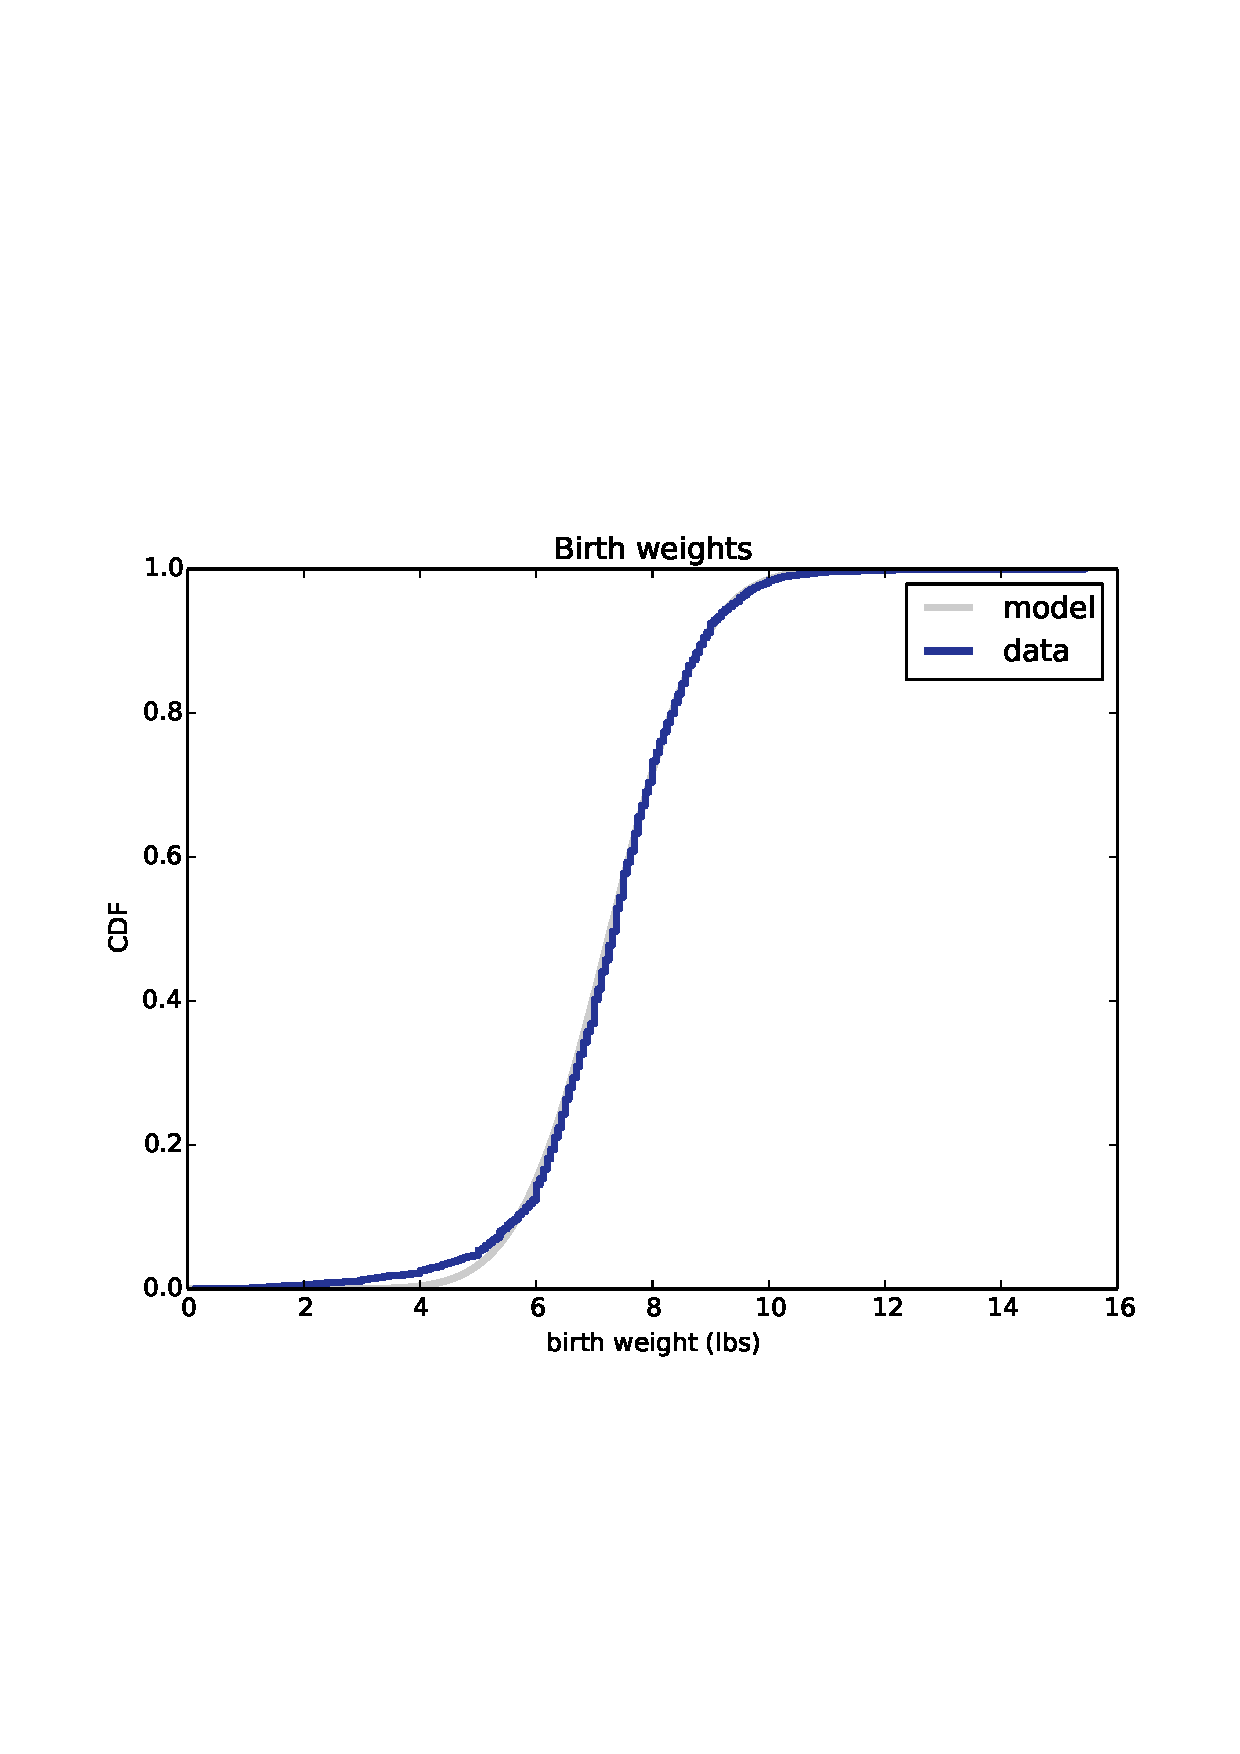
\includegraphics[height=2.5in]{figs/analytic_birthwgt_model.pdf}}
\caption{정규모형과 출생체중 CDF.}
\label{analytic_birthwgt_model}
\end{figure}

정규분포가 이 데이터셋에 대해서 좋은 모형이 된다.
그래서 만약 모수 $\mu = 7.28$과 $\sigma = 1.24$으로 
분포를 요약한다면, 결과 오차(모형과 데이터 간 차이)가 작다.

\index{모형 (model)}
\index{백분위수 (percentile)}

백분위수 10번째 아래에서 데이터와 모형 사이에 불일치가 있다.
정규분포에서 예측되는 것보다 더 많이 체중이 적은 아이가 있다.
만약 조산아에 특별히 관심이 있다면, 분포에서 이 부분을 잘 적합하는 것이 중요하다.
그래서 정규분포를 사용하는 것이 적절하지 않을 수도 있다.


\section{정규확률그림 (Normal probability plot)}

지수분포와 몇가지 분포에서 대해서 해석분포(analytic distribution)가 특정 데이터셋에 대해서
적합한 모형인가를 테스트하는데 사용할 수 있는 간단한 변환이 있다.

\index{지수분포 (exponential distribution)}
\index{분포 (distribution)!지수 (exponential)}
\index{모형 (model)}

정규분포에 대해서 그러한 변환은 없다. 하지만, 
{\bf 정규확률그림 (normal probability plot)}으로 불리는 대안이 있다.
정규확률그림을 생성하는 방식이 두개 있다.: 어려운 방식과 쉬운 방식.
어려운 방식에 관심이 있다면 \url{https://en.wikipedia.org/wiki/Normal_probability_plot}에서 
자세한 정보를 얻을 수 있다.
다음에 쉬운 방식이 있다.
\index{정규확률그림 (normal probability plot)}
\index{그림 (plot)! 정규확률 (normal probability)}
\index{정규분포 (normal distribution)}
\index{분포 (distribution)!정규 (normal)}
\index{가우스 분포 (Gaussian distribution)}
\index{분포 (distribution)!가우스 (Gaussian)}

\begin{enumerate}

\item 표본에 있는 값을 정렬한다.

\item 표준정규분포($\mu=0$, $\sigma=1$)에서 표본과 동일한 크기를 갖는 난수을 생성하고
정렬한다.
\index{난수 (random number)}

\item 표본에서 나온 정렬된 값과 난수를 플롯으로 그린다.

\end{enumerate}

만약 표본 분포가 근사적으로 정규분포라면, 결과는 
절편 {\tt mu}, 기울기 {\tt sigma}를 갖는 직선이다.
{\tt thinkstats2}에 {\tt NormalProbability}이 있다.
표본을 인자로 받아서 넘파이(NumPy) 배열 두개를 반환한다.
\index{넘파이 (NumPy)}

\begin{verbatim}
xs, ys = thinkstats2.NormalProbability(sample)
\end{verbatim}

\begin{figure}
% analytic.py
\centerline{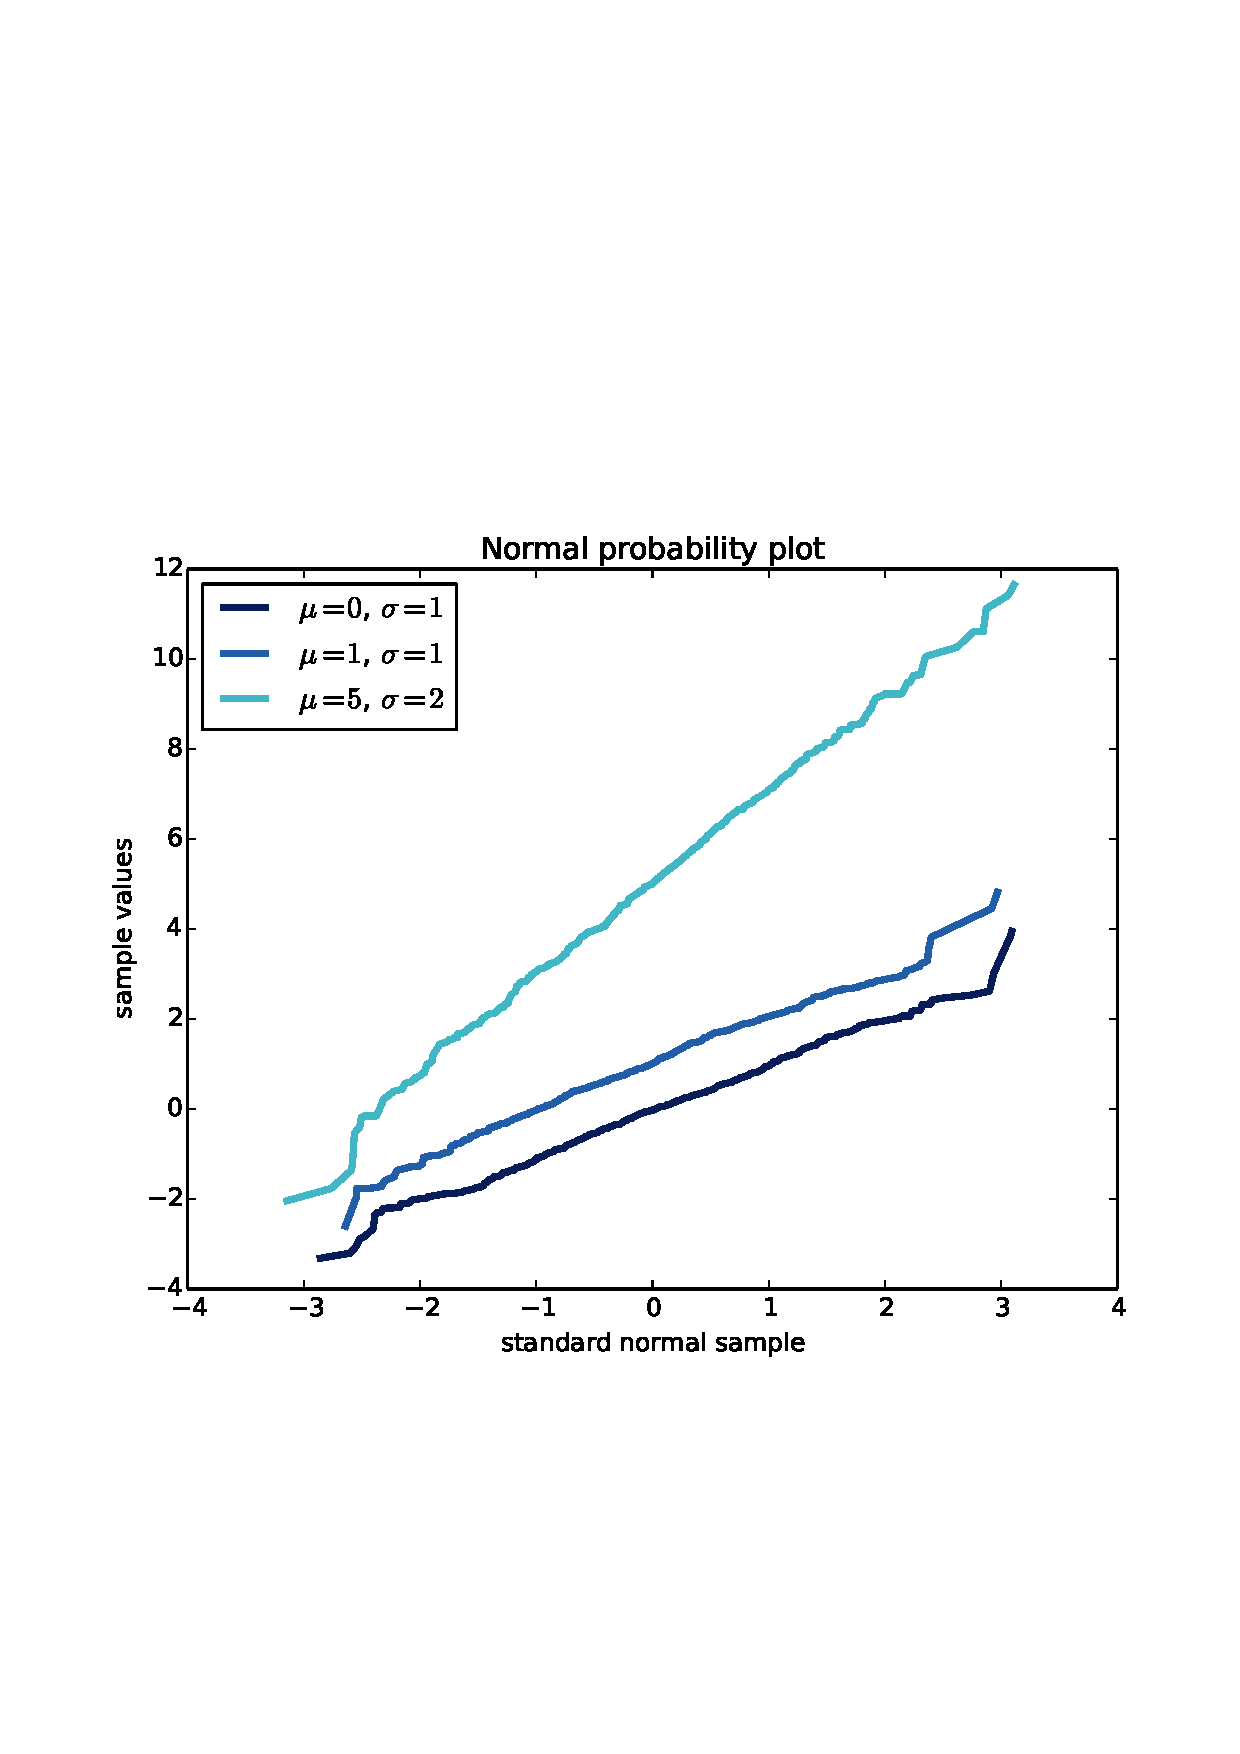
\includegraphics[height=2.5in]{figs/analytic_normal_prob_example.pdf}}
\caption{정규분포에서 나온 임의 표본에 대한 정규확률그림.}
\label{analytic_normal_prob_example}
\end{figure}

{\tt ys}는 {\tt sample}에서 정렬된 값이 담겨있다; 
{\tt xs}에는 표준정규분포에서 생성된 난수가 담겨있다.

{\tt NormalProbability}을 테스트하기 위해서 다양한 모수를 가진 
정규분포에서 모조 샘플을 생성했다.
그림~\ref{analytic_normal_prob_example}에 결과가 있다.
선들이 근사적으로 직선으로, 평균에 있는 값보다 벗어난 값을 꼬리에 갖는다.

이제 실제 데이터에 적합을 시도해 보자.
앞절로부터 출생 체중 데이터에 대해 정규확률그림을 생성하는 코드가 다음에 있다.
모형을 표현하는 회색선과 실제 데이터를 표현하는 파란선을 플롯으로 그린다.

\index{출생 체중 (birth weight)}
\index{체중 (weight)!출생 (birth)}

\begin{verbatim}
def MakeNormalPlot(weights):
    mean = weights.mean()
    std = weights.std()

    xs = [-4, 4]
    fxs, fys = thinkstats2.FitLine(xs, inter=mean, slope=std)
    thinkplot.Plot(fxs, fys, color='gray', label='model')

    xs, ys = thinkstats2.NormalProbability(weights)
    thinkplot.Plot(xs, ys, label='birth weights')
\end{verbatim}

{\tt weights}는 출생 체중 판다스 시리즈다; {\tt mean}과 {\tt std}은
각각 평균과 표준편차다.
\index{판다스 (pandas)}
\index{시리즈 (Series)}
\index{thinkplot}
\index{표준편차 (standard deviation)}

{\tt FitLine}이 시퀀스 {\tt xs}, 절편, 기울기를 인자로 받는다;
반환하는 {\tt xs}와 {\tt ys}는 {\tt xs} 값에서 계산되어 인자로 받은 모수를 가진 직선이다.

{\tt NormalProbability}은 {\tt xs}와 {\tt ys}를 반환하는데 
표준정규분포에서 나온 값과 {\tt weights}에서 나온 값을 담고 있다.
만약 체중 분포가 정규분포를 따른다면, 데이터도 모델과 매칭되어야 한다.

\index{모형 (model)}

\begin{figure}
% analytic.py
\centerline{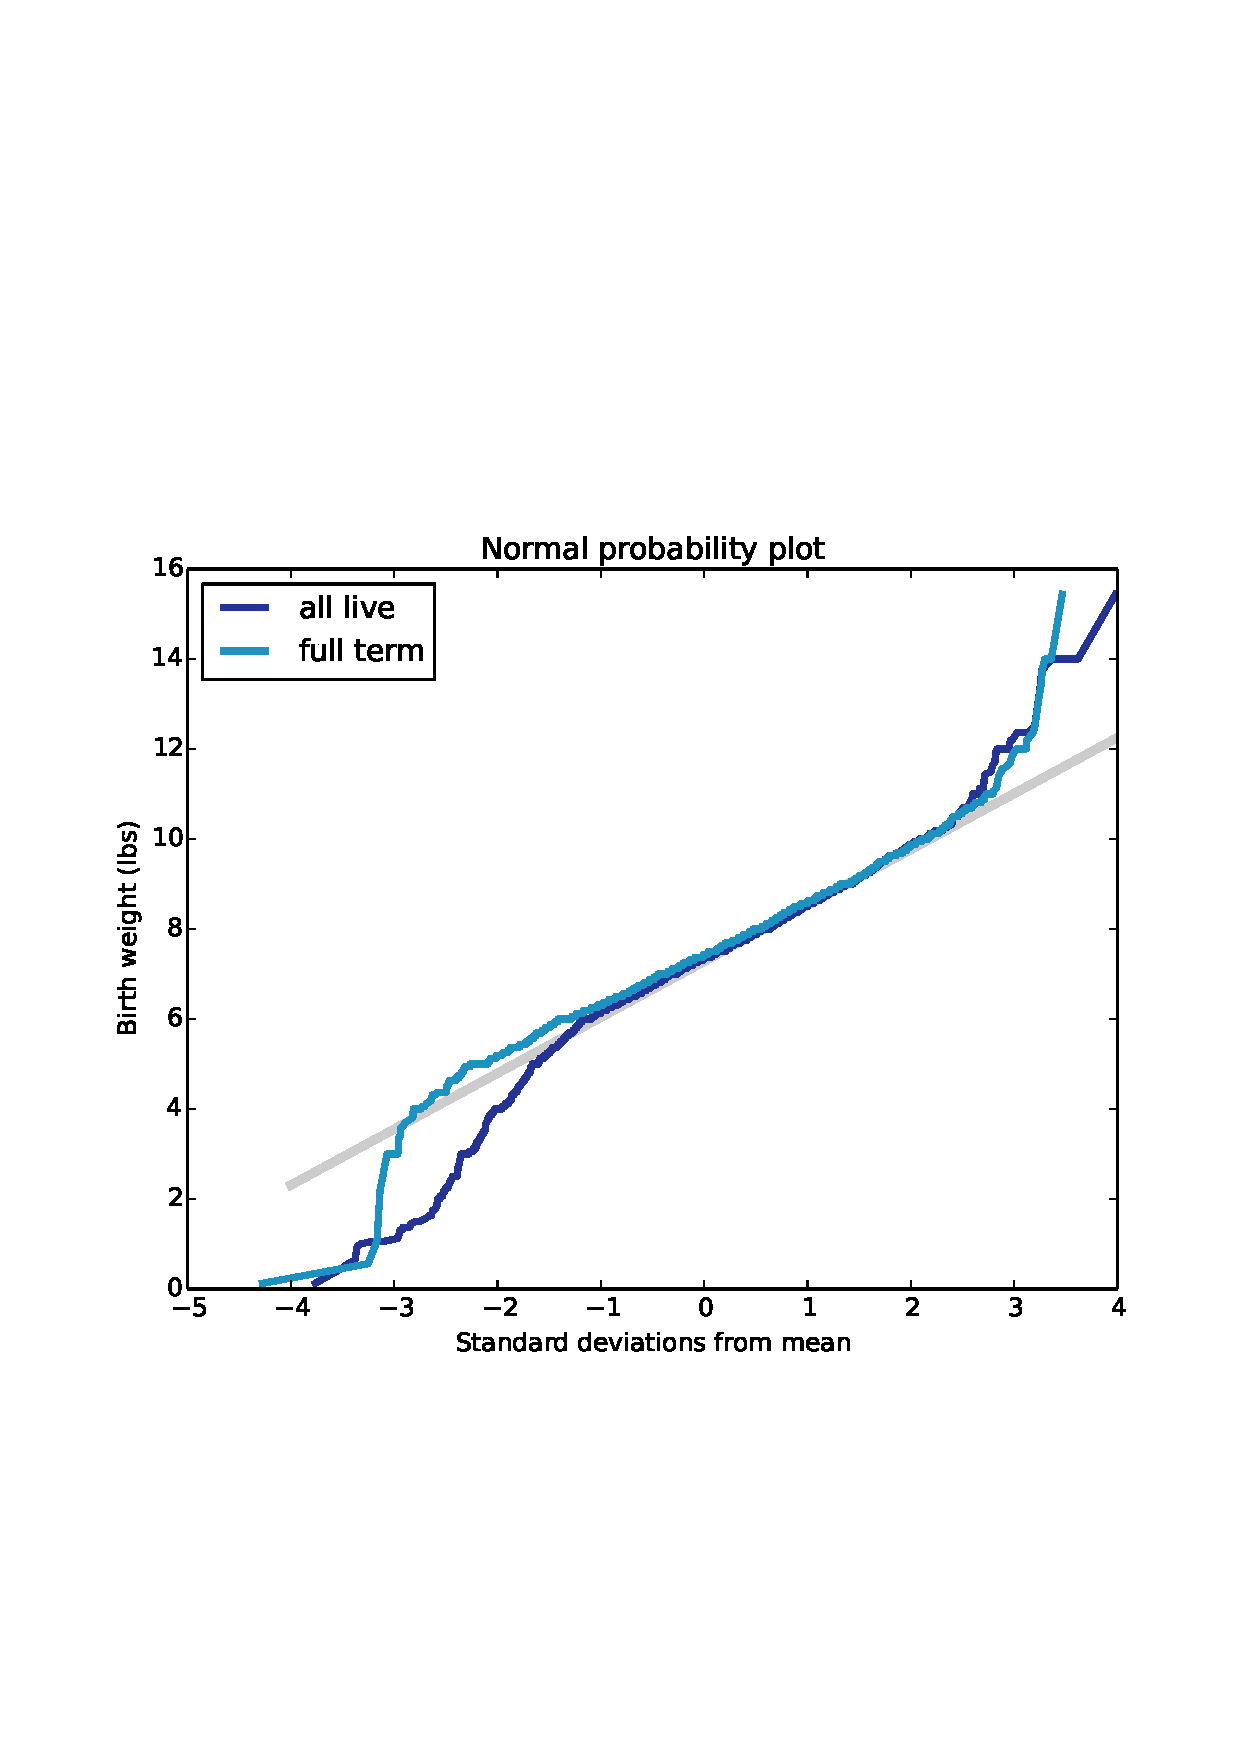
\includegraphics[height=2.5in]{figs/analytic_birthwgt_normal.pdf}}
\caption{출생체중에 대한 정규확률그림.}
\label{analytic_birthwgt_normal}
\end{figure}

그림~\ref{analytic_birthwgt_normal}이 전체 정상 출생과 더불어 만삭(임신기간이 36주 이상)에 대한 결과를 보여준다.
두 곡선 모두 평균 근처에서 모형과 매칭되고 꼬리에서 차이가 난다.
가장 무거운 아이가 모형이 예측한 것보다 더 무겁고, 가장 가벼운 아이는 더 가볍다.

\index{임신 기간}

단지 만삭 아이만 선택해서, 가장 가벼운 몇몇 아이를 제거하면 분포 아래쪽 꼬리에 있는 불일치를 줄일 수 있다.

정규분포 모형이 평균에서부터 몇 표준편차 내에서 분포를 잘 기술하지만, 꼬리 부근에서는 아니라고 플롯 그래프를 통해서 알 수 있다.
실제 목적에 얼마나 부합되는지는 목적에 달려있다.
\index{모형 (model)}
\index{출생 체중 (birth weight)}
\index{체중 (weight)!출생 (birth)}
\index{표준편차 (standard deviation)}


\section{로그 정규분포 (lognormal distribution)}
\label{brfss}
\label{lognormal}

만약 값을 로그 취한 집합이 정규분포라면, 이 값은 {\bf 로그 정규분포 (lognormal distribution)}다. 로그 정규분포 CDF는 $x$를 $\log x$로 치환한 정규분포 CDF와 동일하다.
%
\[ CDF_{lognormal}(x) = CDF_{normal}(\log x)\]
%
로그 정규분포 모수는 일반적으로 $\mu$와 $\sigma$로 표기한다.
하지만, 기억할 것은 모수가 평균과 표준편차는 {\em 아니다};
로그 정규분포 평균은 $\exp(\mu +\sigma^2/2)$이고, 표준편차는 조금 복잡한다.(\url{http://wikipedia.org/wiki/Log-normal_distribution}를 참조한다)
\index{모수 (parameter)} 
\index{체중 (weight)!성인 (adult)} 
\index{성인 체중 (adult weight)}
\index{로그 정규분포 (lognormal distribution)}
\index{분포 (distribution)!로그 정규 (lognormal)}
\index{CDF}

\begin{figure}
% brfss.py
\centerline{
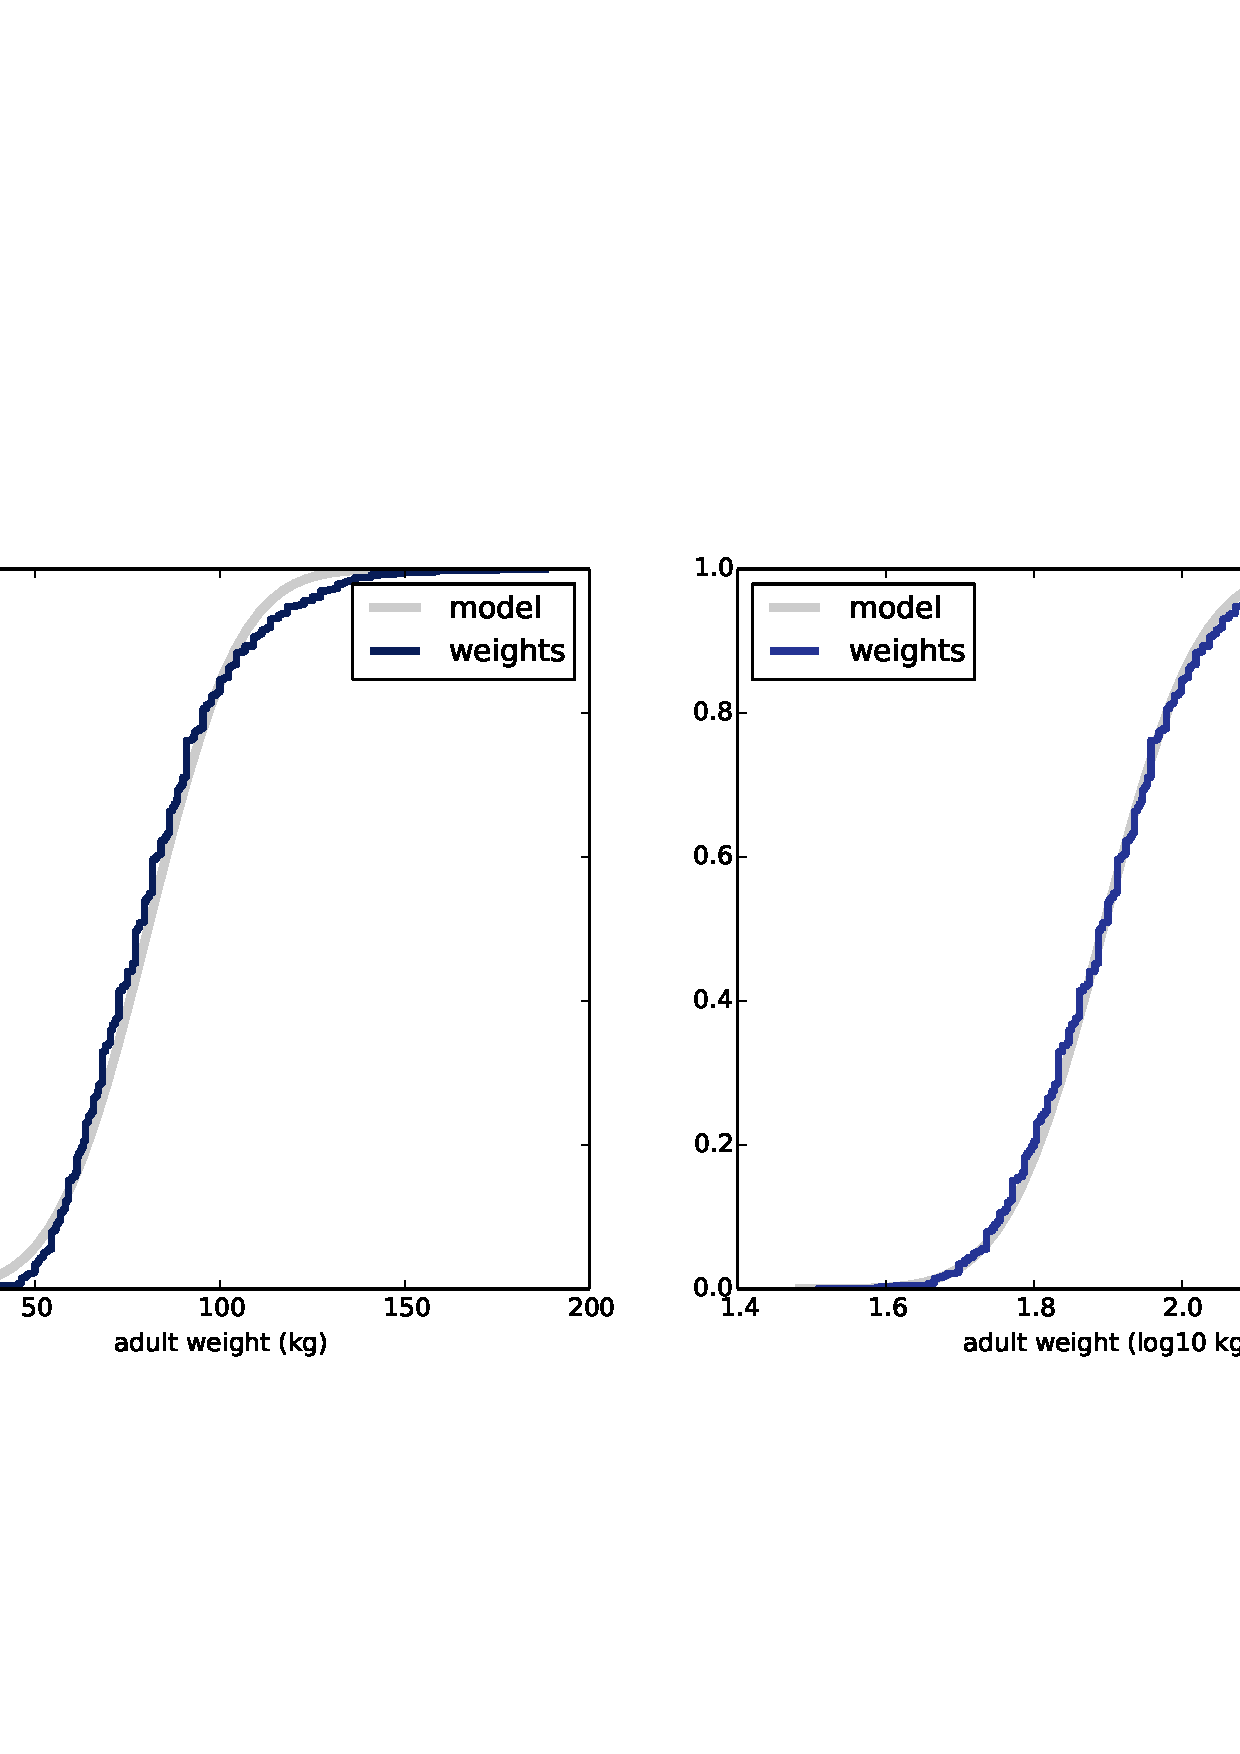
\includegraphics[height=2.5in]{figs/brfss_weight.pdf}}
\caption{선형척도(좌측)와 로그척도(우측)로 본 성인체중에 대한 CDF.}
\label{brfss_weight}
\end{figure}

만약 표본이 근사적으로 로그 정규분포이고 log-x 척도로 CDF 플롯을 그린다면, 정규분포 특성의 형상을 갖는다.
표본이 로그 정규분포 모형과 얼마나 잘 적합하는지 테스트하기 위해서, 
표본값에 로그를 취해서 정규확률그림을 생성할 수 있다.

\index{정규확률그림 (normal probability plot)}
\index{모형 (model)}

예제로 성인 체중 분포를 살펴보는데 근사적으로 로그 정규분포다.\footnote{\url{http://mathworld.wolfram.com/LogNormalDistribution.html} 사이트에서 주석(인용없이)으로 이 가능성에 대해서 제보를 받았다.
나중에 로그 변환과 원인을 제안하는 논문을 발견했다: Penman and Johnson, ``The Changing Shape of the Body Mass Index Distribution Curve in the Population,'' Preventing Chronic Disease, 2006 July; 3(3): A74.  Online at \url{http://www.ncbi.nlm.nih.gov/pmc/articles/PMC1636707}.}


만성 질환 예방 및 건강 증진을 위한 국립 센터 (National Center for Chronic Disease Prevention and Health Promotion)에서는 
행동 위험 요인 감시 시스템(Behavioral Risk Factor Surveillance System, BRFSS)\footnote{질병통제 예방센터(Centers for Disease Control and Prevention, CDC). 행동 위험 요인 감시 시스템 조사 자료(Behavioral Risk Factor Surveillance System Survey Data). Atlanta, Georgia: 미국 보건 복지부 (U.S. Department of Health and Human Services), 질병통제 예방센터 (Centers for Disease Control and Prevention), 2008.}의 일부문으로 매년 조사를 실시한다.
2008년 414,509 응답자를 대상으로 인터뷰했고 인구통계, 건강, 건강 위험에 관해서 설문했다. 수집한 데이터 중에 398,484 응답자 킬로그램으로 표시된 체중정보가 있다.
\index{행동 위험 요인 감시 시스템 (Behavioral Risk Factor Surveillance System)}
\index{BRFSS}

이 책을 위한 저장소에 BRFSS에 관한 데이터를 담고 있는 고정폭 아스키(ASCII)파일, {\tt CDBRFS08.ASC.gz}와 더불어 파일을 읽고 데이터를 분석하는 {\tt brfss.py}파일도 함께 있다.

\begin{figure}
% brfss.py
\centerline{
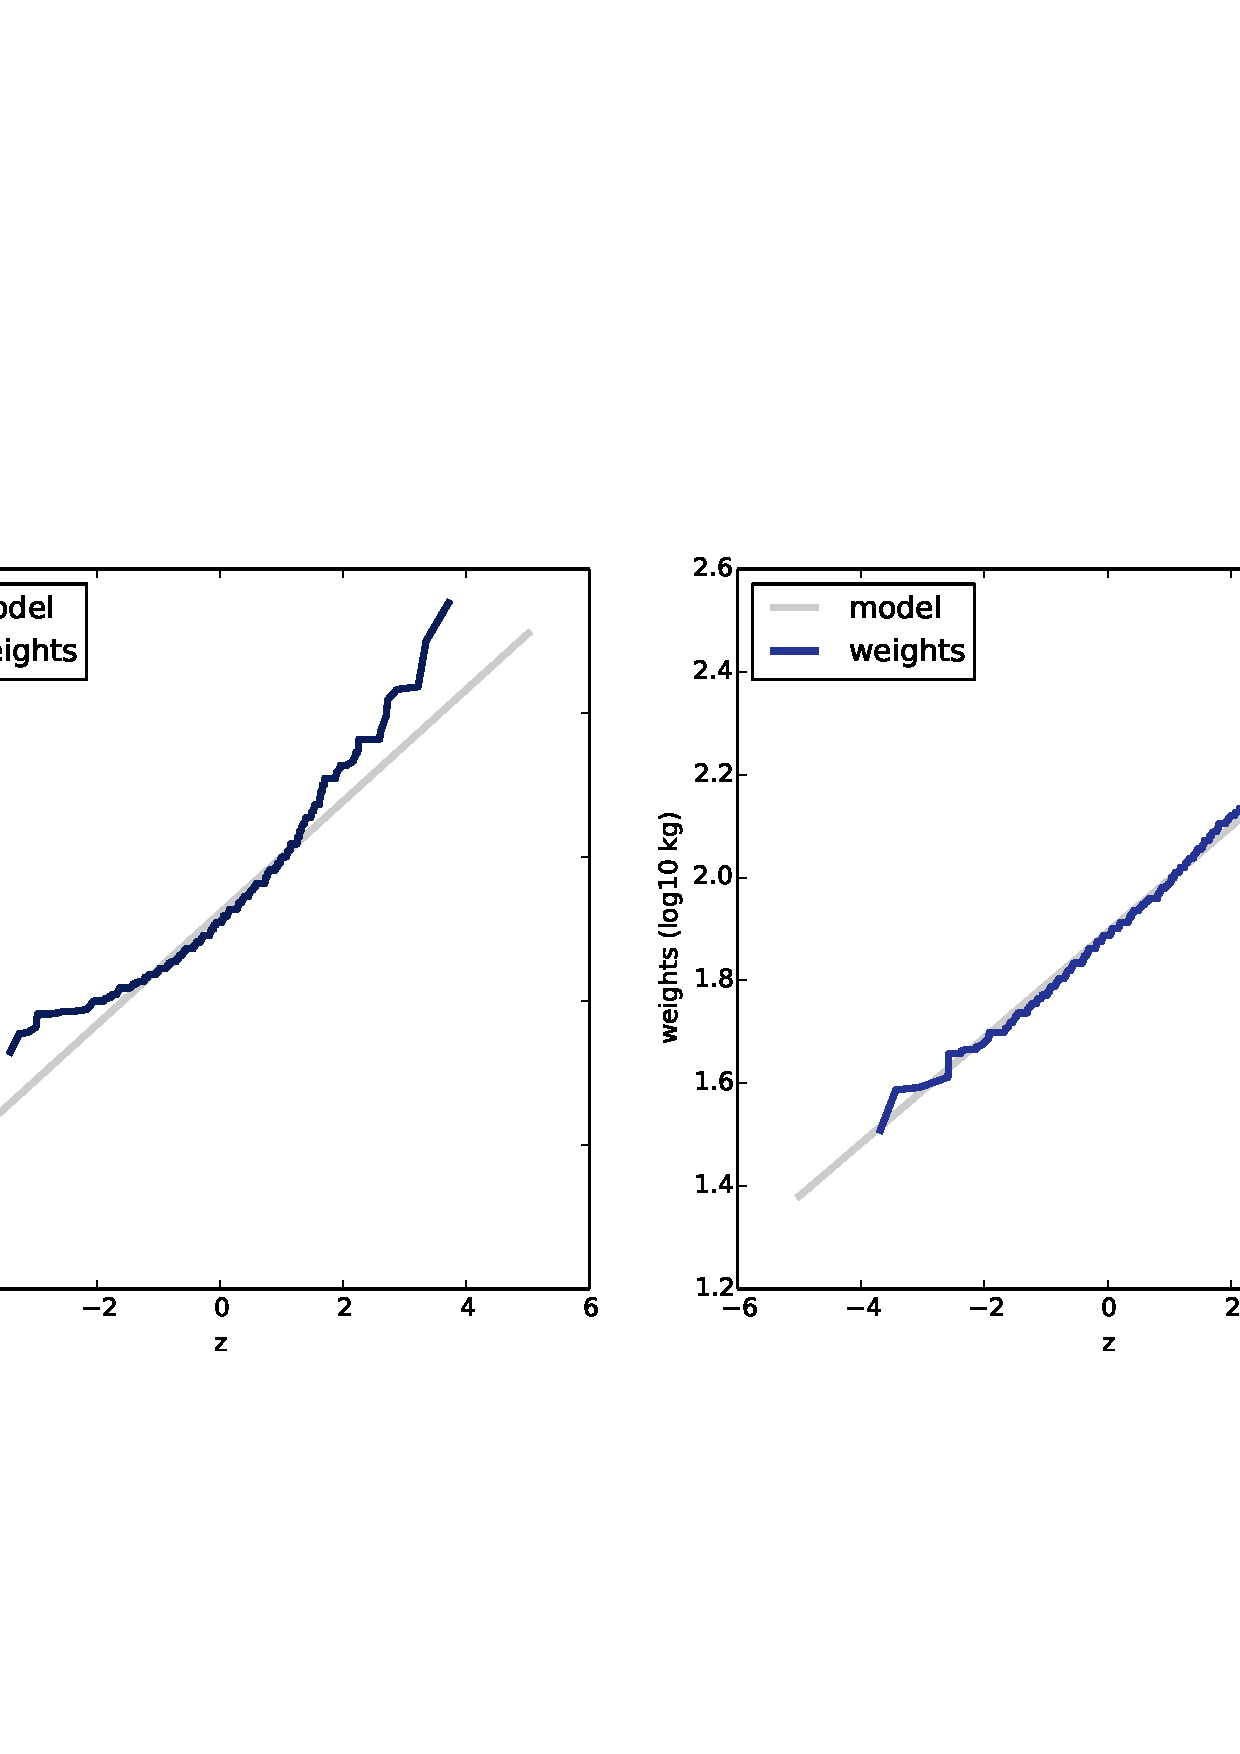
\includegraphics[height=2.5in]{figs/brfss_weight_normal.pdf}}
\caption{선형척도(좌측)와 로그척도(우측)로 본 성인체중에 대한 정규확률그림.}
\label{brfss_weight_normal}
\end{figure}

그림~\ref{brfss_weight} (왼편)이 정규분포 모형에 선형 척도로 성인 체중 분포를 나타낸다.
그림~\ref{brfss_weight} (오른편)이 로그 정규분포 모형으로 로그 척도로 동일한 분포를 나타낸다.
로그 정규 모형이 더 나은 적합이지만 데이터를 이와 같이 표현하는 것이 차이점을 특별히 인상적으로 만들지는 못한다.
\index{응답자 (respondent)} 
\index{모형 (model)}

그림~\ref{brfss_weight_normal}이 성인 체중 $w$에 대한 정규확률그림과 
로그 변환한 체중 $\log_{10} w$에 대한 정규확률그림을 보여준다.
이제 데이터가 정규분포 모형에서 상당히 벗아난 것이 명확하다.
다른 한편으로 로그 정규모형은 데이터에 대한 좋은 매칭을 보여준다.

\index{정규분포 (normal distribution)} 
\index{분포 (distribution)!정규 (normal0}
\index{가우스 분포 (Gaussian distribution)} 
\index{분포 (distribution)!가우스 (Gaussian)}
\index{로그 정규분포 (lognormal distribution)} 
\index{분포 (distribution)!로그 정규 (lognormal)}
\index{표준편차 (standard deviation)} 
\index{성인 체중 (adult weight)} 
\index{체중 (weight)!성인 (adult)}
\index{모형 (model)} 
\index{정규확률그림 (normal probability plot)}


\section{파레토 분포 (Pareto distribution)}
\index{파레토 분포 (Pareto distribution)}
\index{분포 (distribution)!파레토 (Pareto)}
\index{파레토, 빌프레도 (Pareto, Vilfredo)}

{\bf 파레토 분포 (Pareto distribution)}는 경제학자 빌프레도 파레토(Vilfredo Pareto) 이름에서 나왔는데, 이것을 사용해서 부(
\url{http://wikipedia.org/wiki/Pareto_distribution} 참조)의 분포를 기술했다.
그후, 도시와 마을 크기, 모래 입자와 운석, 산불과 지진을 포함한 자연과학과 사회과학 현상을 기술하는데 사용되었다.

\index{CDF}

파레토 분석 CDF는 다음과 같다.
%
\[ CDF(x) = 1 - \left( \frac{x}{x_m} \right) ^{-\alpha} \]
%
모수 $x_{m}$와 $\alpha$이 분포 위치와 형상을 결정한다.
$x_{m}$이 가능한 최소값이다. 
그림~\ref{analytic_pareto_cdf}에 $x_{m} = 0.5$와 
다양한 $\alpha$ 값으로 표현한 파레토 분포 CDF가 있다.
\index{모수 (parameter)}

\begin{figure}
% analytic.py
\centerline{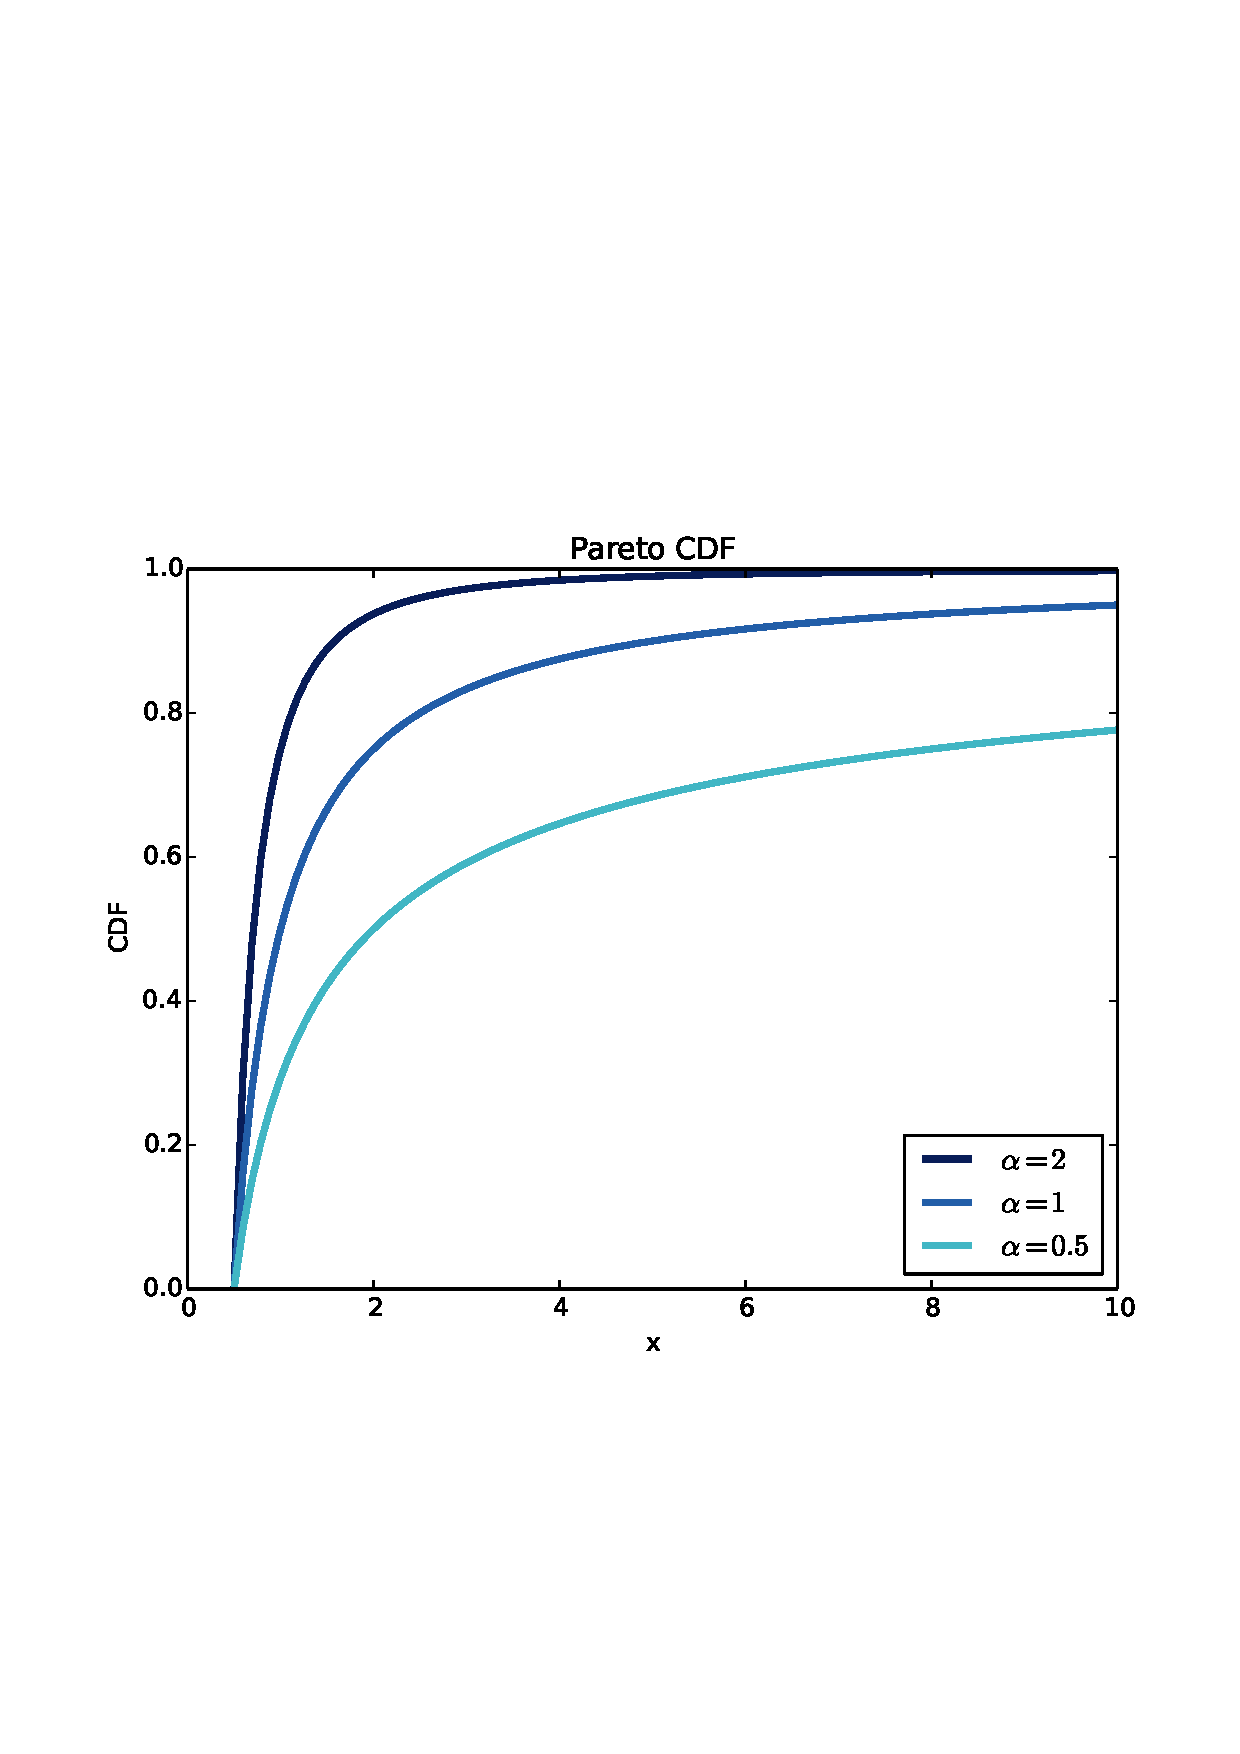
\includegraphics[height=2.5in]{figs/analytic_pareto_cdf.pdf}}
\caption{다른 모수를 갖는 파레토 분포 CDF.}
\label{analytic_pareto_cdf}
\end{figure}

경험적 분포가 파레토 분포에 적합성을 나타내는 간단한 시각 테스트가 있다: log-log 척도에서 CCDF는 직선으로 보인다. 왜 그런지 살펴보자.

만약 선형척도에서 파레토 분포에서 나온 표본 CCDF를 플롯으로 그린다면, 다음과 같은 함수가 기대된다.
%
\[ y \approx \left( \frac{x}{x_m} \right) ^{-\alpha} \]
%
양변에 로그를 취하면 다음과 같다.
%
\[ \log y \approx -\alpha (\log x - \log x_{m})\]
%
그래서 만약 $\log x$에 $\log y$를 플롯으로 그리면, 
기울기 $-\alpha$과 절편 $\alpha \log x_{m}$을 가진 직선처럼 보여야만 한다.

예제로, 도시와 마을 크기를 살펴보자.
미국 인구 조사국 (U.S.~Census Bureau)에서 미국에 있는 모든 도시와 마을 인구정보를 게시한다.
\index{파레토 분포 (Pareto distribution)} 
\index{분포 (distribution)!파레토 (Pareto)}
\index{미국 인구 조사국 (U.S.~Census Bureau)} 
\index{인구 (population)} 
\index{도시 크기 (city size)}

\begin{figure}
% populations.py
\centerline{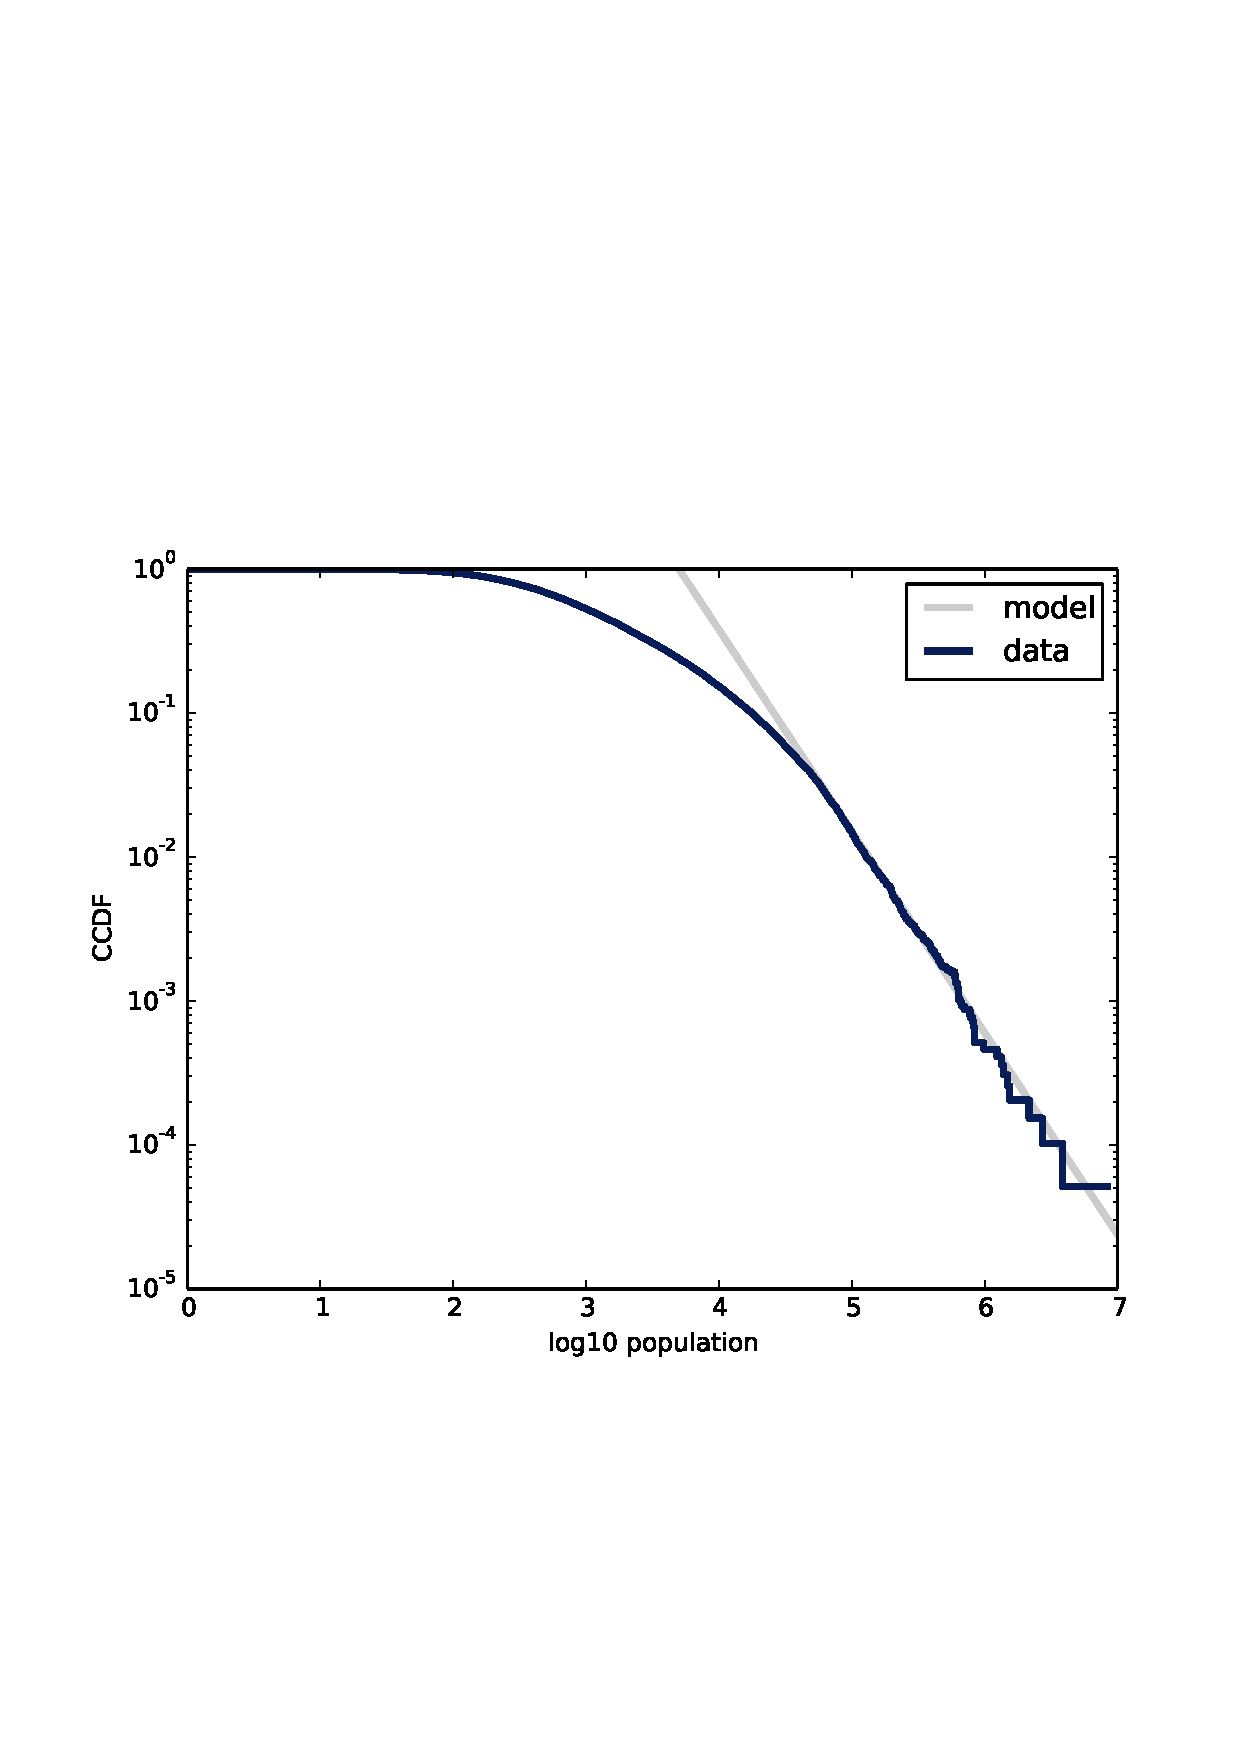
\includegraphics[height=2.5in]{figs/populations_pareto.pdf}}
\caption{로그-로그 척도로 도시 인구 CCDFs.}
\label{populations_pareto}
\end{figure}

웹사이트 \url{http://www.census.gov/popest/data/cities/totals/2012/SUB-EST2012-3.html}에서 데이터를 다운로드했다; 책 저장소에 \verb"PEP_2012_PEPANNRES_with_ann.csv" 파일 이름으로 되어있다.
저장소에 {\tt populations.py} 파이썬 프로그램이 있어 파일을 읽고 인구 분포를 플롯으로 그린다.

그림~\ref{populations_pareto}에 log-log 척도로 인구 CCDF가 있다.
$10^{-2}$ 아래 가장 큰 1\% 도시와 마을이 직선을 따라 아래를 향한다. 몇몇 연구자와 마찬가지로 분포 꼬리가 파레토 모형에 적합하다고 결론을 내릴 수 있다.
\index{모형 (model)}

다른 한편으로 로그 정규분포도 또한 데이터를 잘 모형화한다. 
그림~\ref{populations_normal}에 인구 CDF의 로그 정규분포 모형(왼쪽), 정규확률그림(오른쪽)이 있다. 두 플롯 그림 모두 데이터와 모형 사이 좋은 적합을 보여준다.
\index{정규확률그림 (normal probability plot)}

모형 어느 것도 완벽하지 않다. 파레토 모형은 단지 가장 큰 1\% 도시에만 적용되지만 분포의 그 특정 부분에 더 적합이 잘 된다. 
로그 정규 모형은 99\% 다른 부분에 더 적합이 잘 된다.
어느 모형이 적절한가는 분포 어느 부분에 관련이 있는지에 달려 있다.

\begin{figure}
% populations.py
\centerline{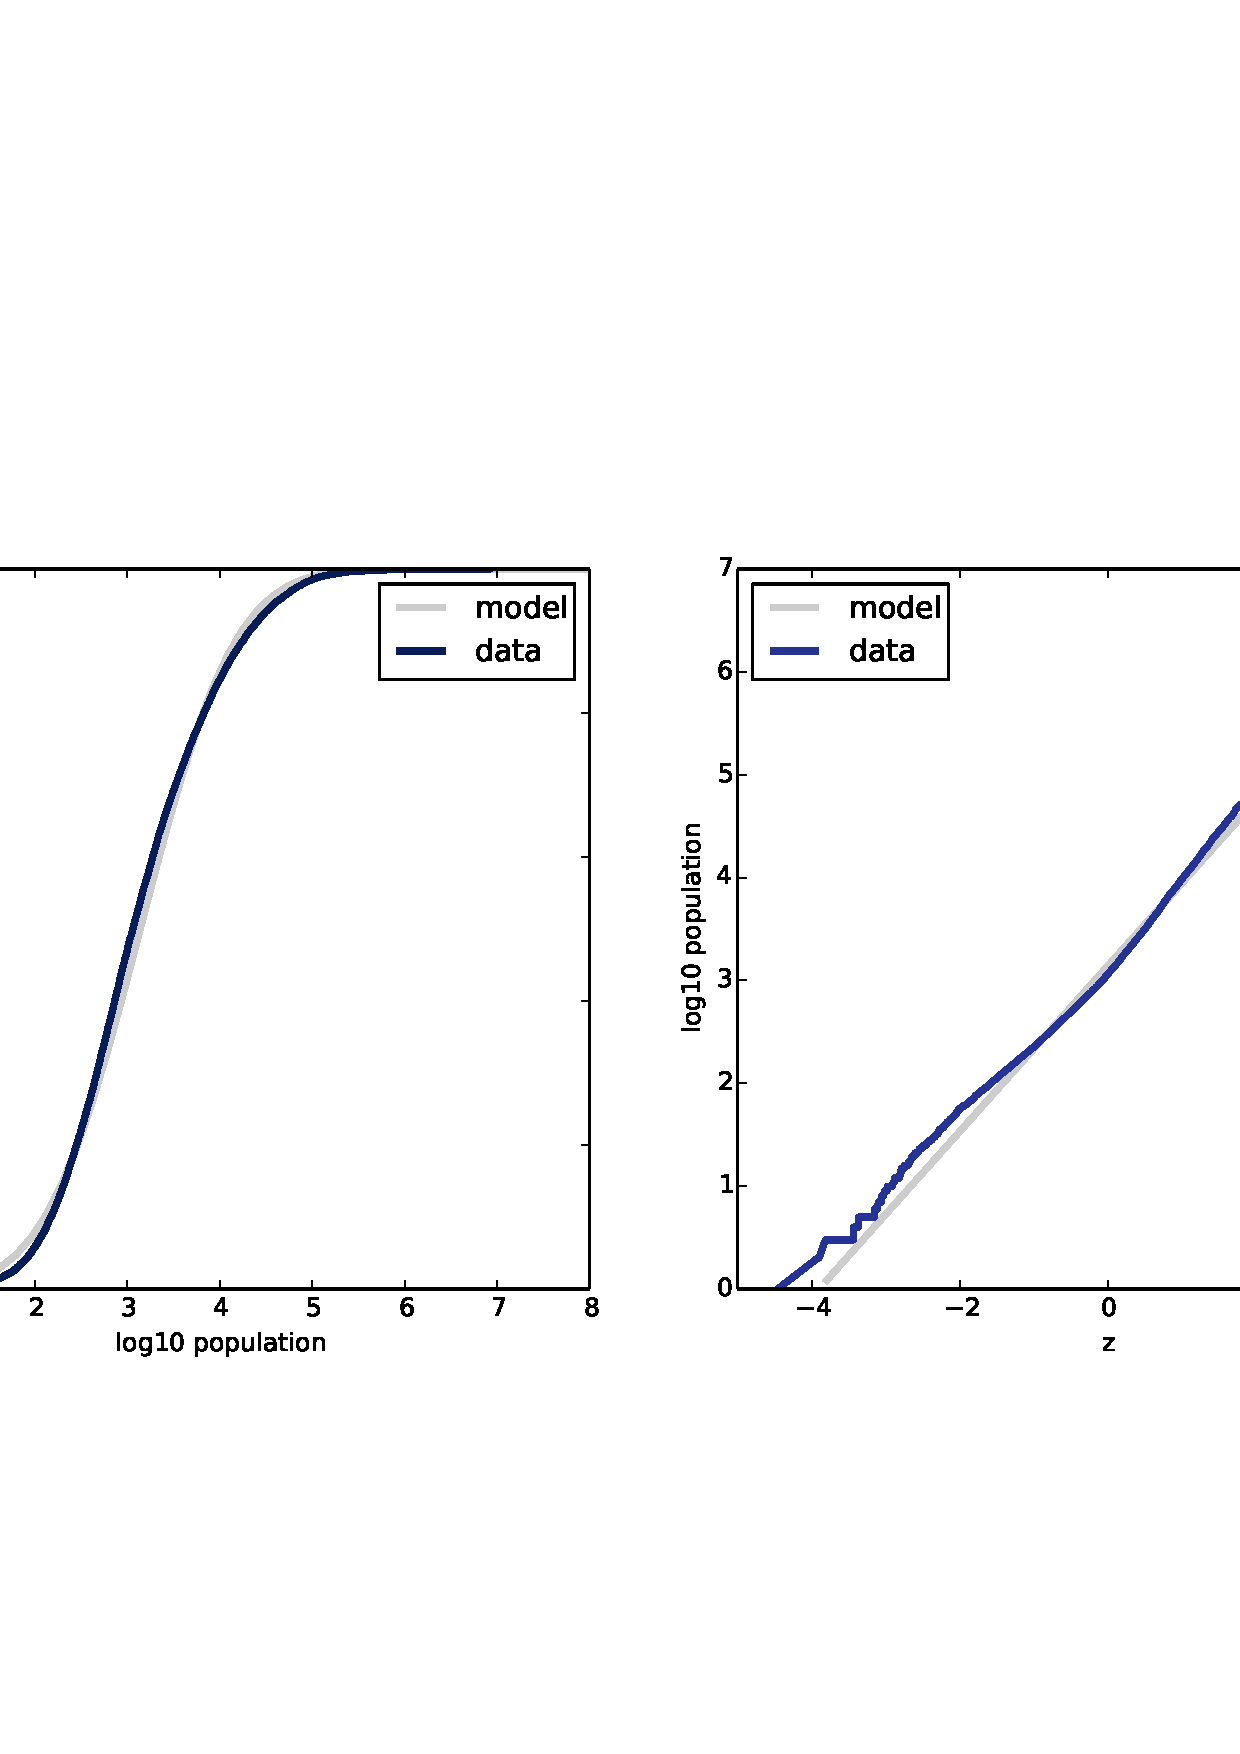
\includegraphics[height=2.5in]{figs/populations_normal.pdf}}
\caption{로그-로그 척도(좌측)로 본 도시인구 CDF, 로그변환 인구(우축)의 정규확률그림.}
\label{populations_normal}
\end{figure}


\section{난수 생성하기 (Generating random numbers)}
\index{지수 분포 (exponential distribution)}
\index{분포 (distribution)!지수 (exponential)}
\index{난수 (random number)}
\index{CDF}
\index{역 CDF 알고리즘 (inverse CDF algorithm)}
\index{균등 분포 (uniform distribution)}
\index{분포 (distribution)!균등 (uniform)}

해석 CDF(analytic CDF)를 사용해서 주어진 분포함수 $p = \CDF(x)$로 난수를 생성한다. 역 CDF를 계산하는 효율적인 방식이 있다면, 
0과 1 사이 균등분포에서 $p$를 선택하고 나서 $x = ICDF(p)$를 선택함으로써 적절한 분포 난수를 생성할 수 있다.
\index{역 CDF (inverse CDF)}
\index{CDF, 역 (CDF, inverse)}

예를 들어 지수분포 CDF는 다음과 같다.
%
\[ p = 1 - e^{-\lambda x} \]
%
$x$에 대해 풀게되면 다음이 된다.
%
\[ x = -\log (1 - p) / \lambda \]
%
그래서 파이썬 코드로 다음과 같이 작성할 수 있다.
%
\begin{verbatim}
def expovariate(lam):
    p = random.random()
    x = -math.log(1-p) / lam
    return x
\end{verbatim}

함수 {\tt expovariate}는 {\tt lam}을 인자로 받아
모수 {\tt lam}인 지수분포에서 생성된 난수를 반환한다.

파이썬 코드 구현에 두가지 주의점이 있다: 
\verb"lambda"가 파이썬 예약어(keyword)여서 모수를 \verb"lam"으로 했다. 또한 $\log 0$가 정의되어 있지 않기 때문에, 약간 더 주의해야 한다.
{\tt random.random} 구현코드는 0을 반환할 수 있지만 1은 할 수 없다.
그래서, $1 - p$은 1이 될 수는 있지만 0은 될 수 없어서 {\tt log(1-p)}은 항상 정의된다. 
\index{랜덤 모듈 (random module)}


\section{왜 모형인가?}
\index{모형 (model)}

이 장의 시작에서 많은 현실 세계 현상이 해석 분포(analytic distribution)으로 모형화될 수 있다고 말했다.
``그래서,'' ``뭐?'' 라고 물을 수도 있다.
\index{추상화 (abstraction)}

모든 모형처럼, 해석분포는 추상화다. 의미하는 바은 관련없다고 판단되는 세부적인 사항을 생략한다는 것이다. 예를 들어, 관찰된 분포에는 표본 특유의 측정오류나 유별난 점이 포함될 수 있다; 해석 모형은 이러한 유별난 점을 매끈하게 평활한다.
\index{평활 (smoothing)}

해석 모형은 또한 일종의 데이터 압축이다. 모형이 테이터셋에 잘 적합될 때, 적은 모수 집합으로 대량의 데이터를 요약할 수 있다.
\index{모수 (parameter)}
\index{압축 (compression)}

때때로, 자연현상에서 나온 데이터가 해석 분포에 잘 적합되는 것을 보면 참 놀랍니다. 하지만, 이같은 관찰이 물리적 시스템에 대한 통찰(insight)을 제공한다.
때때로 관측된 분포가 왜 특별한 형태를 갖는지 설명할 수 있다.
예를 들어, 파레토 분포는 긍정적 피드백을 생성하는 과정(generative process)의 결과다 (소위 선호적 연결 과정 (preferential attachment processes): \url{http://wikipedia.org/wiki/Preferential_attachment} 사이트를 참조.)
\index{선호적 연결 (preferential attachment)}
\index{생성하는 과정 (generative process)}
\index{파레토 분포 (Pareto distribution)}
\index{분포 (distribution)!파레토 (Pareto)}
\index{해석 (analysis)}

또한, \ref{analysis}~장에서 살펴보듯이 해석 분포가 수학적 분석으로 이끈다. 

하지만, 모든 모형이 완전하지 않다는 것을 기억하는 것이 중요하다.
현실 세계에서 나온 데이터는 결코 완벽하게 해석 분포에 적합되지 않는다. 종종 사람들이 데이터가 모형에서 생성된 것처럼 말을 한다; 예를 들어, 사람 신장분포가 정규분포에서 나왔다거나 소득 분포가 로그정규분포에서 나왔다고 말한다. 문자 그대로 받아들이면, 이러한 주장은 진실이 아니다; 항상 현실 세계와 수학적 모형 사이에는 차이가 있다.

현실 세계의 중요한 측면을 포착하고 불필요한 세부사항을 배제하면 모형은 유용하다. 하지만, ``중요하거나(relevant)'' ``불필요한(unneeded)'' 것은 모형을 사용해서 무엇을 계획중인가에 달려있다.

\section{연습문제}

아래 연습문제에 대해서, \verb"chap05ex.ipynb" 파일로 시작할 수 있다.
저자 해답은 \verb"chap05soln.ipynb" 파일에 나와 있다.


\begin{exercise}

BRFSS(\ref{lognormal}~절 참조)에서, 
신장 분포의 경우 남자는 $\mu = 178$ cm, $\sigma = 7.7$ cm
여자는 $\mu = 163$ cm, $\sigma = 7.3$ cm을 모수로 갖는 정규분포다.

\index{정규분포}
\index{분포!정규}
\index{가우스 분포}
\index{분포!가우스}
\index{신장}
\index{블루 맨 그룹}
\index{그룹, 블루 맨}

블루 맨 그룹(Blue Man Group)에 가입하기 위해서는 
5'10'' 에서 6'1'' 사이 남자여야 한다(\url{http://bluemancasting.com} 참조). 
미국 남성 인구의 어느 정도 비율이 이 범위에 있는가?
힌트: {\tt scipy.stats.norm.cdf}을 사용한다.
\index{SciPy}

\end{exercise}


\begin{exercise}
파레토 분포에 대한 감각을 갖기 위해서,
만약 사람 신장의 분포가 파레토라면 세상이 얼마나 달라지는지 살펴보자.
$x_{m} = 1$ m, $\alpha = 1.7$ 모수로, 일리있는 최소값 1 m, 중위수 1.5 m 를 갖는 
분포가 된다.

\index{신장}
\index{파레토 분포}
\index{분포!파레토}

상기 분포를 도식화하세요. 파레토 세상에서 평균 사람 신장은 얼마인가?
인구의 얼마나 평균보다 더 적은가?
만약 파레토 세상에 70억 사람이 있다면, 얼마나 많은 사람들이 1 km 보다
더 클 것으로 예상하는가? 가장 작은 사람은 신장이 얼마나 될 것으로 예상하는가?
\index{파레토 세상}

\end{exercise}


\begin{exercise}
\label{weibull}

와이불 분포(Weibull distribution)는 고장 분석에서 나오는 지수분포를 일반화한 것이다
(\url{http://wikipedia.org/wiki/Weibull_distribution} 참조). CDF는 다음과 같다.
%
\[ CDF(x) = 1 - e^{-(x / \lambda)^k} \]
%
와이블 분포를 직선처럼 보이게 하는 변환을 찾을 수 있을까요?
직선의 기울기와 절편은 무엇을 나타내는가?
\index{와이블 분포}
\index{분포!와이블}
\index{지수 분포}
\index{분포!지수}
\index{random 모듈}

{\tt random.weibullvariate}을 사용해서 와이블 분포에서 표본을 생성하시오.
그리고 이를 사용해서 분포를 테스트하시오.

\end{exercise}


\begin{exercise}
$n$의 적은 값으로, 정확하게 해석 분포에 적합되는
경험분포를 기대하지 못한다.
적합 품질을 평가하는 한 방법이 해석적 분포로부터 표본을 생성하고 
데이터와 얼마나 잘 매칭되는지 살펴보는 것이다.

\index{경험분포}
\index{분포!경험}
\index{random 모듈}

예를 들어, \ref{exponential}~절에서,
출생사이 시간 분포를 도식화했고 근사적으로 지수분포라는 것을 보았다.
하지만, 분포는 단지 데이터가 44에 불과하다.
데이터가 지수분포에서 나왔는지 살펴보기 위해서,
출생사이 약 33분인, 데이터와 동일한 평균을 갖는 지수분포에서 데이터를 44개 생성한다.

임의 확률 표본의 분포를 도식화하고, 실제 분포와 비교한다.
{\tt random.expovariate} 을 사용해서 값을 생성한다.

\end{exercise}

\begin{exercise}
이책을 위한 저장소에서, {\tt mystery0.dat}, 
{\tt mystery1.dat}, 등으로 불리는 데이터 파일을 찾을 수 있다.
해석분포에서 나온 난수열을 각 파일이 담고 있다.

\index{난수}

\verb"test_models.py" 파일도 찾을 수 있는데, 이 파일은
파일에서 데이터를 읽고 다양한 변환으로 CDF를 도식화한다.
다음과 같이 실행할 수 있다:

\begin{verbatim}
$ python test_models.py mystery0.dat
\end{verbatim}

도식화된 결과에 기반해서, 어떤 유형의 분포가 각 파일을 생성했는지 추론할 수 있어야 한다.
만약 막힌다면, {\tt mystery.py} 파일을 살펴보는데, 파일을 생성한 코드가 담겨있다.

\end{exercise}


\begin{exercise}
\label{income}

부와 소득의 분포를 종종 로그정규분포와 파레토 분포로 모형화한다.
어느 것이 더 나은지 알아내기 위해서, 데이터를 들여다 보자.
\index{파레토 분포}
\index{분포!파레토}
\index{로그정규 분포}
\index{분포!로그정규}

인구동향조사(Current Population Survey, CPS)는 노동통계국(Bureau of Labor Statistics)과 
인구조사국(Census Bureau)의 공동작업으로 소득과 관련된 변수를 연구한다.
2013년에 수집된 데이터는 \url{http://www.census.gov/hhes/www/cpstables/032013/hhinc/toc.htm}에서 다운로드 받을 수 있다.
저자는 가구소득 정보를 갖는 엑셀 파일 {\tt hinc06.xls} 을 다운로드 받아서,
이책의 저장소에서 찾을 수 있는 CSV 파일 {\tt hinc06.csv}로 변환했다.
이 CSV 파일을 불러읽는 {\tt hinc.py} 파일도 함께 있다.

\index{인구동향조사}
\index{노동통계국}
\index{인구조사국}

이 데이터셋에서 소득분포를 추출하라. 이번 장에서 학습한 어떤 해석분포가 데이터에 대해 좋은 모형이 되는가?
이 연습문제에 대한 해답은 \url{hinc_soln.py} 파일에 나와 있다.
\index{모형}

\end{exercise}




\section{용어 사전}

\begin{itemize}

\item 경험적 분포 (empirical distribution): 표본 값의 분포 
\index{경험적 분포 (empirical distribution)} 
\index{분포 (distribution)!경험적 (empirical)}

\item 해석 분포 (analytic distribution): CDF가 해석함수인 분포.
\index{해석 분포 (analytic distribution)}
\index{분포 (distribution)!해석 (analytic)}

\item 모형 (model): 유용한 단순화. 해석 분포는 종종 많이 복잡한 경험적 분포에 대한 좋은 모형이다.
\index{모형 (model)}

\item 도착간격시간 (interarrival time): 두 사건 사이 경과 시간.
\index{도착간격시간 (interarrival time)}

\item 보완 CDF (complementary CDF): 
값 $x$에서 $x$를 넘는 값 비율로 매칭하는 함수, $1 - \CDF(x)$.
\index{보완 CDF (complementary CDF)} 
\index{CDF!보완 (complementary)} 
\index{CCDF}

\item 표준정규분포 (standard normal distribution): 
평균 0과 표준편차 1을 갖는 정규분포.
\index{표준정규분포 (standard normal distribution)}

\item 정규확률그림 (normal probability plot): 표본값과 표준정규분포에서 나온 난수를 대비하여 플롯하여 그린 그림.
\index{정규확률그림 (normal probability plot)}
\index{그림 (plot)!정규확률 (normal probability)}

\end{itemize}



\chapter{확률밀도함수}
\label{density}
\index{PDF}
\index{확률밀도함수 (probability density function)}
\index{지수분포 (exponential distribution)}
\index{분포 (distribution)!지수 (exponential)}
\index{정규분포 (normal distribution)}
\index{분포 (distribution)!정규 (normal)}
\index{가우스 분포 (Gaussian distribution)}
\index{분포 (distribution)!가우스 (Gaussian)}
\index{CDF}
\index{미분 (derivative)}


이번 장에서 사용되는 코드는 {\tt density.py}에 있다.
코드를 다운로드하고 작업하는 것에 대한 정보는 ~\ref{code}을 참조한다.

\section{PDF}

CDF 미분을 {\bf 확률밀도함수 (probability density function)}, PDF라고 한다.
예를 들어, 지수분포 PDF는 다음과 같다.

%
\[ \PDF_{expo}(x) = \lambda e^{-\lambda x}   \]
%
정규분포 PDF는 다음과 같다.
%
\[ \PDF_{normal}(x) = \frac{1}{\sigma \sqrt{2 \pi}} 
                 \exp \left[ -\frac{1}{2} 
                 \left( \frac{x - \mu}{\sigma} \right)^2 \right]  \]
%

$x$ 특정한 값에 대한 PDF를 계산하는 것이 대체로 유용하지는 않다. 결과가 확률이 아니기 때문이다; 확률 {\em 밀도 (density)}다.
\index{밀도 (density)}
\index{질량 (mass)}

물리학에서 밀도는 단위 체적당 질량이다; 질량을 계산하려면, 체적을 곱하거나 혹은 만약 밀도가 상수가 아니라면 체적에 대해 적분해야 한다.

마찬가지로, {\bf 확률 밀도 (probability density)}는 단위 $x$당 확률을 측정한다. 확률 질량을 계산하려면, $x$에 대해서 적분해야 한다. 

{\tt thinkstats2}는 Pdf라는 클래스로 확률밀도함수를 나타낸다.
모든 Pdf 객체는 다음 메쏘드를 제공한다:

\begin{itemize}

\item {\tt Density}, {\tt x}를 인자로 받아 {\tt x}에서 분포 밀도를 반환한다.

\item {\tt Render}는 이산 집합값 대해 밀도를 평가하고 시퀀스 짝을 반환한다: 정렬된 {\tt xs}과 상응하는 확률 밀도{\tt ds}.

\item {\tt MakePmf}, 이산 집합값에 대해 {\tt Density}를 평가하고 Pdf에 그사하는 정규화된 Pmf를 반환한다.
\index{Pmf}

\item {\tt GetLinspace}, {\tt Render}와 {\tt MakePmf}에서 사용되는 기본설정 집합 점(point)을 반환한다.

\end{itemize}  

Pdf는 추상화된 부모 클래스로 의미하는 것은 인스턴스화하면 안된다; 즉, Pdf 객체를 생성할 수 없다. 대신에 Pdf를 상속받아 {\tt Density}과 {\tt GetLinspace} 정의하는 자식 클래스를 정의해야 한다. 
Pdf는 {\tt Render}과 {\tt MakePmf}을 제공한다.

예를 들어, {\tt thinkstats2}는 정규밀도함수를 평가하는 {\tt NormalPdf}라는 이름의 클래스를 제공한다.

\begin{verbatim}
class NormalPdf(Pdf):

    def __init__(self, mu=0, sigma=1, label=''):
        self.mu = mu
        self.sigma = sigma
        self.label = label

    def Density(self, xs):
        return scipy.stats.norm.pdf(xs, self.mu, self.sigma)

    def GetLinspace(self):
        low, high = self.mu-3*self.sigma, self.mu+3*self.sigma
        return np.linspace(low, high, 101)
\end{verbatim}

NormalPdf 객체는 모수 {\tt mu}과 {\tt sigma}을 담고 있다.
{\tt Density}는 {\tt scipy.stats.norm}을 사용하는데 정규분포를 표현한고, 
다른 메쏘드와 더불어 {\tt cdf}와 {\tt pdf}를 제공한다.(~\ref{normal}절 참조).
\index{SciPy}

다음 예제는 BRFSS에 있는 성인여성신장(cm 단위) 평균과 분산으로 NormalPdf를 생성한다(~\ref{brfss}절 참조). 그리고 나서, 평균에서 1 표준편차 지점에 분포 밀도를 계산한다.
\index{표준 편차 (standard deviation)}

\begin{verbatim}
>>> mean, var = 163, 52.8
>>> std = math.sqrt(var)
>>> pdf = thinkstats2.NormalPdf(mean, std)
>>> pdf.Density(mean + std)
0.0333001
\end{verbatim}

결과는 cm 당 확률질량 단위로 약 0.03이다.
한번더, 확률밀도는 그 자체로 의미는 없다. 하지만, Pdf를 플롯으로 그린다면, 분포 형상을 볼 수 있다.

\begin{verbatim}
>>> thinkplot.Pdf(pdf, label='normal')
>>> thinkplot.Show()
\end{verbatim}

{\tt thinkplot.Pdf}은 평활 함수(smooth function)로 Pdf 플롯을 그린다. 
계단함수로 Pmf을 그리는 {\tt thinkplot.Pmf}와 대조된다.
그림~\ref{pdf_example}에 결과가 있다. 다음 절에서 살펴볼 표본에서 추정한 PDF로 함께 플롯되어 그려져 있다.
\index{thinkplot}

Pdf를 근사하는데 {\tt MakePmf}를 사용할 수도 있다.

\begin{verbatim}
>>> pmf = pdf.MakePmf()
\end{verbatim}

기본설정으로, {\tt mu - 3*sigma}에서 {\tt mu + 3*sigma} 사이에 동일 간격을 지닌 101 점이 Pmf에 있다.
선택사양으로 {\tt MakePmf}와 {\tt Render}는 키워드 인자로 {\tt low}, {\tt high}, {\tt n}을 갖는다.

\begin{figure}
% pdf_example.py
\centerline{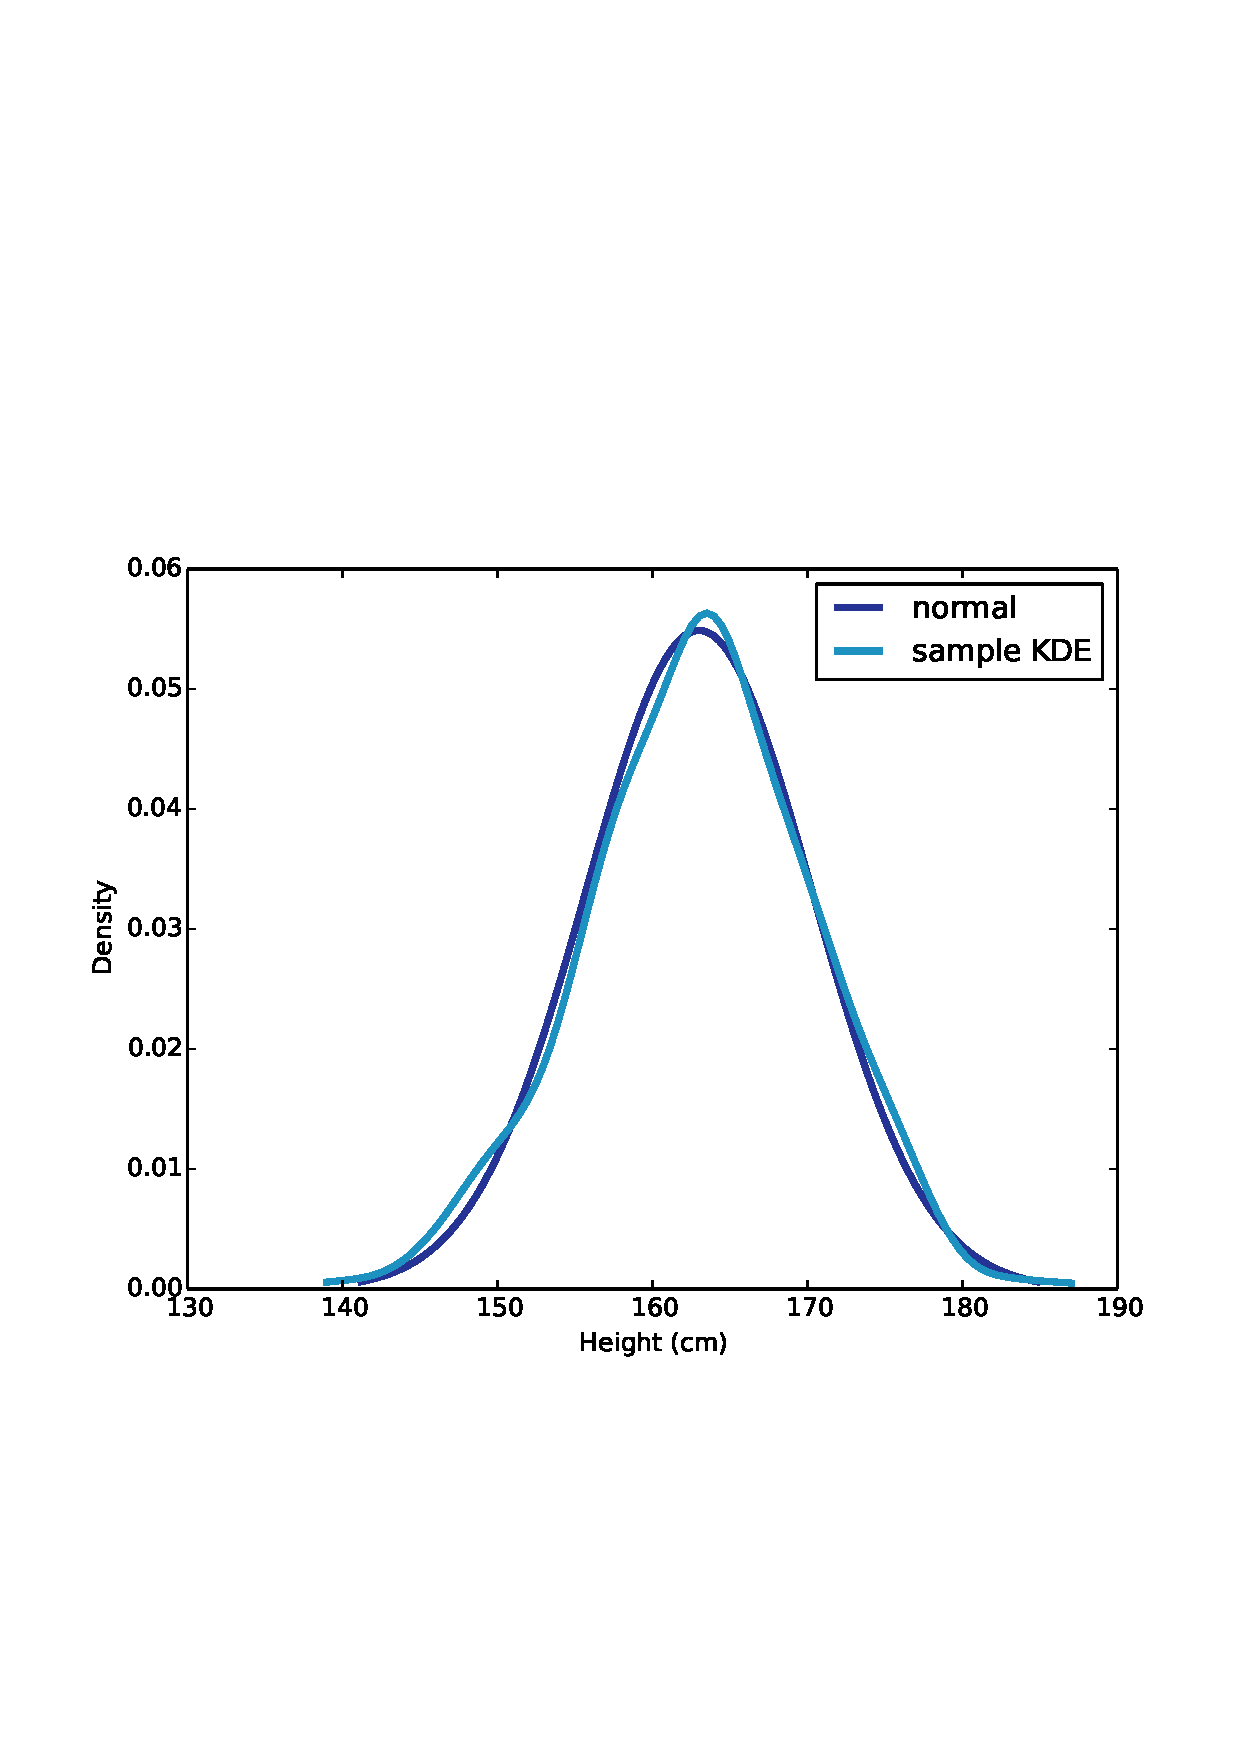
\includegraphics[height=2.2in]{figs/pdf_example.pdf}}
\caption{미국 성인 여성 신장을 모형화하는 정규 PDF, 그리고 $n=500$ 표본으로 핵밀도추정.}
\label{pdf_example}
\end{figure}


\section{핵밀도추정 (Kernel density estimation)} 

{\bf 핵밀도추정 (Kernel density estimation,KDE)}은
표본을 받아 데이터에 적합하는 적절한 평활 PDF를 찾는 알고리즘이다.
\url{http://en.wikipedia.org/wiki/Kernel_density_estimation}  웹사이트에서 좀더 자세한 정보를 얻을 수 있다.

\index{KDE}
\index{핵밀도추정 (kernel density estimation)}

{\tt scipy}에 KDE 구현된 것이 있고, 
{\tt thinkstats2}는 이를 사용해서 {\tt EstimatedPdf}라는 클래스를 제공한다.
\index{사이파이 (SciPy)}
\index{넘파이 (NumPy)}

\begin{verbatim}
class EstimatedPdf(Pdf):

    def __init__(self, sample):
        self.kde = scipy.stats.gaussian_kde(sample)

    def Density(self, xs):
        return self.kde.evaluate(xs)
\end{verbatim}

\verb"__init__"이 표본을 인자로 받아 핵밀도추정값을 계산한다.
결과는 \verb"gaussian_kde" 객체고 {\tt evaluate} 메쏘드를 제공한다.

{\tt Density}가 값 혹은 시퀀스를 인자로 받아 
\verb"gaussian_kde.evaluate"을 호출하고 결과 밀도를 반환한다.
단어 ``가우스 (Gaussian)''가 나오는데 이유는 KDE를 평활하는데 가우스 분포에 기반한 필터를 사용하기 때문이다.
\index{밀도 (density)}

다음에 정규분포에서 표본을 생성하고 표본에 적합하기 위해서 EstimatedPdf를 만드는 예제가 있다.
\index{넘파이 (NumPy)}
\index{EstimatedPdf}

\begin{verbatim}
>>> sample = [random.gauss(mean, std) for i in range(500)]
>>> sample_pdf = thinkstats2.EstimatedPdf(sample)
>>> thinkplot.Pdf(sample_pdf, label='sample KDE')
\end{verbatim}

\verb"sample"은 무작위 신장 500개 리스트다. 
\verb"sample_pdf"는 Pdf 객체로 추정된 KDE 표본정보를 담고 있다.
동일 간격 값의 시퀀스에서 밀도를 평가함으로써 {\tt pmf}는 Pmf 객체로 Pdf를 근사한다.

그림~\ref{pdf_example}에 정규밀도함수와 무작위 신장 500개 표본에 기반한 KDE가 있다. 추정값이 원분포에 좋은 매칭이다.

KDE로 밀도함수를 추정하는 것은 몇가지 목적으로 유용한다. 

\index{thinkplot}
\index{Pmf}

\begin{itemize}

\item {\it 시각화 (Visualization):} 
  프로젝트 탐색단계에서, CDF가 대체로 분포를 가장 잘 시각화한다.
  CDF를 살펴본 후에, 추정 PDF가 분포에 대한 적절한 모형인지 결정할 수 있다.
  만약 그렇다면, CDF에 익숙하지 않은 관계에게 분포를 제시하는데 더 좋은 선택지가 될 수 있다.
\index{시각화 (visualization)}
\index{모형 (model)}

\item {\it 보간 (Interpolation):} 
  추정 PDF는 표본에서 모집단 모형으로 가는 한 방법이다.
  만약 모집단 분포가 매끄럽다고 믿을 이유가 있다면, KDE를 사용해서 표본에 없는 값에 대해 밀도를 보간한다.
\index{보간 (interpolation)}

\item {\it 모의실험 (Simulation):} 
  모의실험은 종종 표본 분포에 기반한다. 
  만약 표본크기가 작다면, KDE를 사용해서 표본분포를 평활하는 것이 적절하다.
  관측점을 중복하기 보다 KDE가 모의실험을 통해서 좀더 가능한 결과값을 탐색하도록 한다.
\index{모의실험 (simulation)}

\end{itemize}


\section{분포 프레임워크 (distribution framework)}
\index{분포 프레임워크 (distribution framework)}

\begin{figure}
\centerline{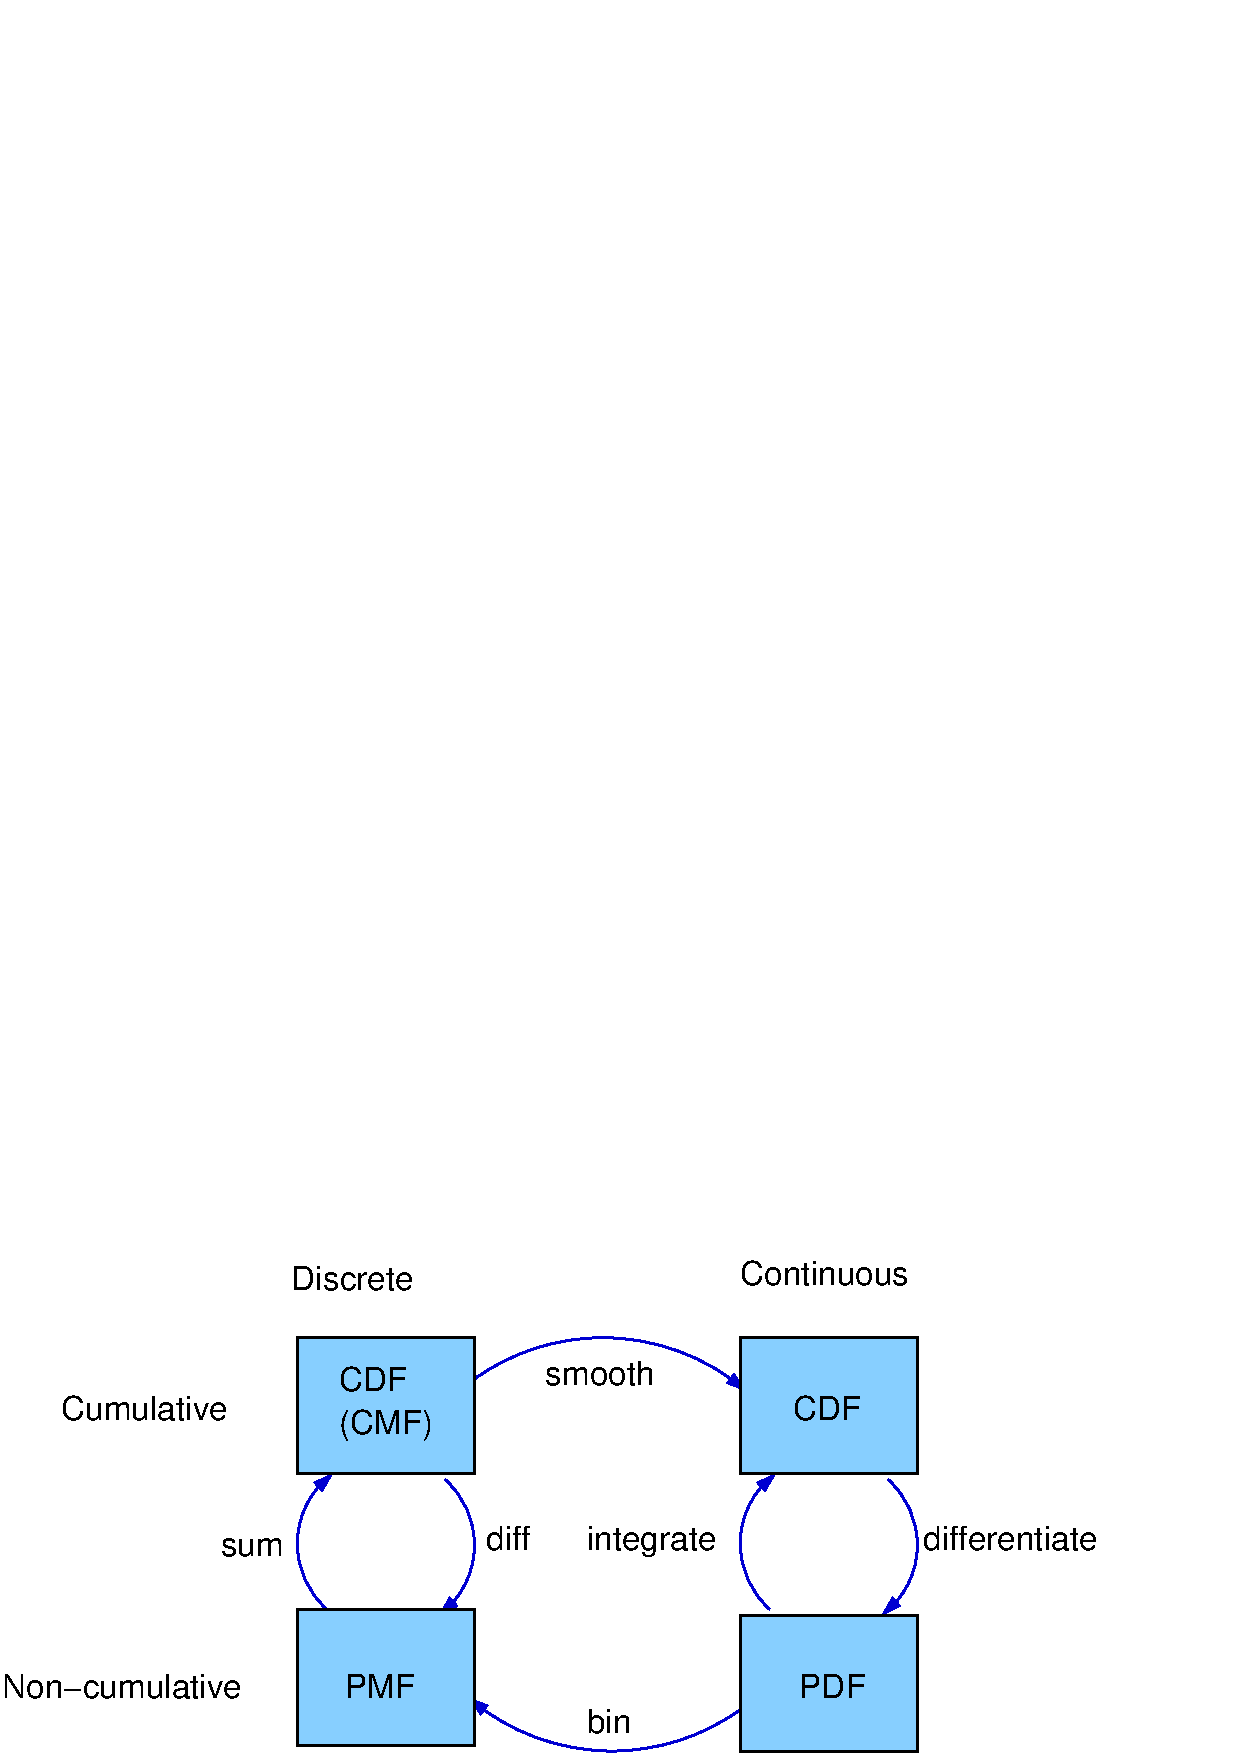
\includegraphics[height=2.2in]{figs/distribution_functions.pdf}}
\caption{분포함수 표현을 연결하는 얼개(framework).}
\label{dist_framework}
\end{figure}

현재까지 PMF, CDF, PDF를 살펴봤다; 잠시 복습 시간을 가져본다.
그림~\ref{dist_framework}에 함수가 어떻게 서로 연관되는지 나타나 있다.
\index{Pmf}
\index{Cdf}
\index{Pdf}

PMF로 시작했는데, PMF는 이산 집합 값에 대한 확률을 나타낸다.
PMF에서 CDF를 얻기 위해서는, 확률 질량을 더해서 누적 확률을 얻는다.
CDF에서 PMF로 돌아가기 위해서는, 누적 확률 차이를 계산한다.
다음 몇 절에 걸쳐 이와 같은 연산을 어떻게 구현했는지 살펴볼 것이다.
\index{누적 확률 (cumulative probability)}

PDF는 연속형 CDF 미분이다; 혹은, 동등하게 CDF는 PDF의 적분이다.
PDF는 값을 확률 밀도로 매핑한다는 것을 기억하라; 확률값을 얻기 위해서,
적분해야 한다.

\index{이산 분포 (discrete distribution)}
\index{연속 분포 (continuous distribution)}
\index{평활 (smoothing)}

이산형에서 연속 분포를 얻기 위해서, 다양한 평활(smoothing) 작업을 수행할 수 있다.
평활의 한 형태는 데이터가 (지수 혹은 정규 분포처럼) 
해석 연속 분포(analytic continuous distribution)에서 왔다고 가정하는 것이다.
또 다른 선택 옵션은 핵밀도추정(kernel density estimation)이다.

\index{지수 분포 (exponential distribution)}
\index{분포 (distribution)!지수 (exponential)}
\index{정규 분포 (normal distribution)}
\index{분포 (distribution)!정규 (normal)}
\index{가우스 분포 (Gaussian distribution)}
\index{분포 (distribution)!가우스 (Gaussian)}

평활의 반대가 {\bf 이산화 (discretizing)}, 혹은 양자화(quantizing)다.
만약 이산 점에서 PDF를 평가한다면, PDF에 근사하는 PMF를 생성할 수 있다.
수치적분(numerical integration)을 사용해서 좀더 잘 근사할 수도 있다.
\index{이산화 (discretize)}
\index{양자화 (quantize)}
\index{구간화 (binning)}

연속CDF와 이산CDF를 구별하기 위해서, 이산CDF는 
``누적 질량 함수 (cumulative mass function)''가 되는 것이 좋을지도 모른다.
하지만, 저자가 알고 있는 바로는, 누구도 그 용어를 사용하지 않는다.
\index{CDF}

\section{Hist 구현}

{\tt thinkstats2}에서 제공되는 기본 기능 사용법을 알아야 한다: Hist, Pmf, Cdf, and Pdf.
다음 절에는 구현된 방식에 대한 상세한 정보가 나와있다.
학습 교재가 좀더 효율적으로 이들 클래스를 사용하는지 도움을 줄 수 있지만,
엄격히 말해서 반듯이 필요하지는 않다.
\index{Hist}

Hist와 Pmf는 \verb"_DictWrapper"라는 부모 클래스를 상속받는다.
클래스 앞 밑줄은 클래스가 ``내부(internal)''라는 것을 나타낸다; 즉,
다른 모듈에 코드로 사용되면 않된다. 명칭이 무엇인지 나타낸다: 
딕셔너리 랩퍼(dictionary wrapper). 
주요 속성은 {\tt d}로, 값을 빈도로 매핑하는 딕셔너리다.

\index{DictWrapper}
\index{내부 클래스 (internal class)}
\index{랩퍼 (wrapper)}

값은 임의 해쉬형(hashable type)이 될 수 있다.
빈도는 정수형이어야 하지만, 임의 숫자형도 될 수 있다.
\index{해쉬 (hashable)}

\verb"_DictWrapper"는 Hist와 Pmf에 대한 적절한 메쏘드를 담고 있는데,
\verb"__init__", {\tt Values}, {\tt Items}, {\tt Render}가 포함된다.
{\tt Set}, {\tt Incr}, {\tt Mult}, {\tt Remove} 변경 메쏘드도 제공한다.
모든 메쏘드는 딕셔너리 연산으로 구현되었다. 예를 들어,
\index{딕셔너리 (dictionary)}

\begin{verbatim}
# class _DictWrapper

    def Incr(self, x, term=1):
        self.d[x] = self.d.get(x, 0) + term

    def Mult(self, x, factor):
        self.d[x] = self.d.get(x, 0) * factor

    def Remove(self, x):
        del self.d[x]
\end{verbatim}

Hist는 또한 {\tt Freq}을 제공하는데 주어진 값에 대한 빈도를 찾는다.
\index{빈도 (frequency)}

Hist 연산자와 메쏘드는 딕셔너리에 기반하고 있어서, 
이들 메쏘드는 상수 시간 연산이다; 즉, Hist가 점점 커짐에 따라 실행시간이 증가하지 않는다.
\index{Hist}


\section{Pmf 구현}
Pmf가 정수 빈도 대신에 값을 부동소수점 확률에 매핑하는 것을 제외하고, 
Pmf와 Hist는 거의 동일하다.
확률을 다 더한 합계가 1 이라면, Pmf는 정규화되었다.
\index{Pmf}

Pmf는 {\tt Normalize} 함수를 제공하는데, 확률을 합을 계산하고 갯수로 나눈다.

\begin{verbatim}
# class Pmf

    def Normalize(self, fraction=1.0):
        total = self.Total()
        if total == 0.0:
            raise ValueError('Total probability is zero.')

        factor = float(fraction) / total
        for x in self.d:
            self.d[x] *= factor

        return total
\end{verbatim}

{\tt fraction}이 정규화한 후에 확률 합계를 알아낸다; 기본 설정값은 1 이다.
만약 전체 확률이 0 이라면, Pmf는 정규화될 수 없어서, {\tt Normalize}는 {\tt ValueError} 오류를 일으킨다.

Hist와 Pmf는 동일한 생성자를 갖고 있다.
인자로 {\tt dict}, Hist, Pmf 혹은 Cdf, 
판다스 시리즈, (값, 빈도) 리스트 쌍, 혹은 값 시퀀스를 받을 수 있다.
\index{Hist}

만약 Pmf를 인스턴스화 한다면, 결과는 정규화된다.
만약 Hist를 인스턴스화 한다면, 결과는 정규화되지 않는다.
정규화되지 않은 Pmf를 생성하기 위해서, 빈 Pmf를  생성해서 변경할 수 있다. Pmf 변경자는 Pmf를 다시 정규화하지 않는다.

\section{Cdf 구현}

CDF가 값을 누적 확률로 매핑해서 Cdf를 \verb"_DictWrapper"로 구현할 수 있다. 하지만 CDF에 있는 값은 정렬되어 있고 \verb"_DictWrapper"에 있는 값은 정렬되어 있지 않다.
또한, 역 CDF를 계산하는 것은 유용하다; 즉, 누적 확률에서 값으로 매핑. 그래서, 저자가 선택한 구현 방법은 두 정렬된 리스트다.
이런 방식으로 이진검색을 사용해서 로그 시간에 앞으로 혹은 역으로 조회할 수 있다.

\index{Cdf}
\index{이진 검색 (binary search)}
\index{누적 확률 (cumulative probability)}
\index{DictWrapper}
\index{역 CDF (inverse CDF)}
\index{CDF, 역 (CDF, inverse)}

Cdf 생성자는 인자로 값 시퀀스 혹은 판다스 시리즈, 값에서 확률로 매핑하는 딕셔너리, (값, 확률) 시퀀스 쌍, Hist, Pmf, 혹은 CDF를 받는다. 혹은 만약 인자가 두개 주어진다면, 두 인자를 각각 정렬된 값 시퀀스와 상응하는 누적확률 시퀀스로 처리한다.

시퀀스, 판다스 시퀀스, 혹은 딕셔너리가 주어지면, 생성자가 Hist를 만든다. 그리고 나서 Hist를 사용해서 속성을 초기화한다.

\begin{verbatim}
        self.xs, freqs = zip(*sorted(dw.Items()))
        self.ps = np.cumsum(freqs, dtype=np.float)
        self.ps /= self.ps[-1]
\end{verbatim}

{\tt xs}는 정렬된 리스트 값이다; {\tt freqs}는 상응하는 빈도 리스트다. {\tt np.cumsum}이 누적 빈도 합계를 계산한다. 
전체 빈도로 나누면 누적확률이 된다.
{\tt n}개 값에 대해서, Cdf를 생성하는 시간은 $n \log n$에 비례한다.
\index{빈도 (frequency)}

다음에 {\tt Prob} 구현한 코드가 있다. 값을 받아 누적 확률을 반환한다.

\begin{verbatim}
# class Cdf
    def Prob(self, x):
        if x < self.xs[0]:
            return 0.0
        index = bisect.bisect(self.xs, x)
        p = self.ps[index - 1]
        return p
\end{verbatim}

{\tt bisect} 모듈은 이진 검색 구현을 제공한다.
그리고, {\tt Value}를 구현했는데 누적 확률을 받아 상응하는 값을 반환한다.

\begin{verbatim}
# class Cdf
    def Value(self, p):
        if p < 0 or p > 1:
            raise ValueError('p must be in range [0, 1]')

        index = bisect.bisect_left(self.ps, p)
        return self.xs[index]
\end{verbatim}

Cdf가 주어지면, 연속 누적 확률 (consecutive cumulative probabilities) 사이 차이를 계산해서 Pmf를 계산할 수 있다.
Cdf 생성자를 호출하고 Pmf를 전달한다면, 
{\tt Cdf.Items}를 호출해서 차이를 계산한다.

\index{Pmf}
\index{Cdf}

\begin{verbatim}
# class Cdf
    def Items(self):
        a = self.ps
        b = np.roll(a, 1)
        b[0] = 0
        return zip(self.xs, a-b)
\end{verbatim}

{\tt np.roll}는 {\tt a} 요소를 오른쪽으로 이동하고,
마지막을 처음으로 ``돌린다(roll)''
{\tt b} 첫 요소를 0으로 바꾸고 나서 {\tt a-b} 차이를 계산한다.
결과는 넘파이 확률 배열이다. 
\index{넘파이 (NumPy)}

Cdf는 {\tt Shift}와 {\tt Scale}를 제공한다. 
Cdf에 값을 변경하지만, 확률은 불변형(immutable)으로 처리되어야 한다.

\section{적률 (Moments)}
\index{적률 (moment)}

어느 때고 표본을 얻고 하나의 숫자로 줄일 수 있다. 그 숫자가 통계량(statistic)이다.
지금까지 살펴본 통계량은 평균, 분산, 중위수, 그리고 사분위수다.

{\bf 원적률 (raw moment)}은 일종의 통계량이다. 만약 $x_i$ 표본 값이 있다면,
$k$번째 원적률은 다음과 같다.

%
\[ m'_k = \frac{1}{n} \sum_i x_i^k \]
%
혹은, 파이썬 표기법으로 표현하면, 다음과 같다.

\begin{verbatim}
def RawMoment(xs, k):
    return sum(x**k for x in xs) / len(xs)
\end{verbatim}

$k=1$일 때, 결과는 표본 평균 $\xbar$가 된다.
다른 원적률은 그 자체로 의미가 있지 않다. 하지만, 다른 계산에 사용된다.

{\bf 중심적률(central moments)}이 더 유용하다. 
$k$번째 중심적률은 다음과 같다.
%
\[ m_k = \frac{1}{n} \sum_i (x_i - \xbar)^k \]
%

혹은 파이썬으로 표현하면 다음과 같다.

\begin{verbatim}
def CentralMoment(xs, k):
    mean = RawMoment(xs, 1)
    return sum((x - mean)**k for x in xs) / len(xs)
\end{verbatim}

$k=2$일 때, 결과는 두번째 중심 적률로 분산으로 인지하고 있을 것이다.
분산의 정의가 왜 이러한 통계량이 적률로 불리는지 힌트를 준다.
각 위치 $x_i$에 자를 따라 추를 달고 평균 주위에서 자를 돌리면, 
회전추의 관성 적률은 값의 분산이다. 만약 관성 적률에 익숙하지 않다면,
\url{http://en.wikipedia.org/wiki/Moment_of_inertia} 웹사이트를 참조한다.  
\index{관성 적률(moment of inertia)}

적률에 기반한 통계를 보고할 때, 단위(unit)에 관한 생각이 중요하다.
예를 들어, 값 $x_i$가 cm 이라면, 첫 원적률은 또한 cm이다.
하지만, 두번째 적률은 cm$^2$이고, 세번째 적률은 cm$^3$... 등등이 된다.

이러한 단위 때문에, 적률은 그 자체로 해석하기 어렵다.
두번째 적률에 대해서 분산에 제곱근을 취한 표준편차를 쓰는 것이 이러한 이유다. 
그러면 $x_i$와 단위가 같아진다.
\index{표준 편차 (standard deviation)}


\section{왜도 (Skewness)}
\index{왜도 (skewness)}

{\bf 왜도 (Skewness)}는 분포 형태를 기술하는 속성이다. 
만약 분포가 중심 경향성 주변에서 대칭이라면, 기울어지지 않았다.
만약 값들이 오른쪽으로 좀더 뻗어져 있다면, ``오른쪽으로 기울어져 (right
skewed)'' 있고, 만약 값들이 왼쪽으로 치우쳐 있다면, ``왼쪽으로 기울어져 (left
skewed''있다.

\index{중심 경향성 (central tendency)}

``기울어짐 (skewed)''을 사용하는 것다는 것이 ``편의(biased)''를 함축하지는 않는다.
단지 왜도는 분포 형태만을 기술한다; 표본 추출과정에 편의가 있는지에 관해 
어떤 것도 나타내지 않는다.

\index{편의 (bias)}
\index{표본 왜도 (sample skewness)}

흔히 몇몇 통계량이 분포 왜도를 계량화하는데 사용된다.
주어진 값 시퀀스가 $x_i$가 주어졌을 때, 
{\bf 표본 왜도 (sample skewness)} $g_1$은 다음과 같이 계산된다.

\begin{verbatim}
def StandardizedMoment(xs, k):
    var = CentralMoment(xs, 2)
    std = math.sqrt(var)
    return CentralMoment(xs, k) / std**k

def Skewness(xs):
    return StandardizedMoment(xs, 3)
\end{verbatim}

$g_1$은 제3 표준 적률로 정규화되었다는 것으로 단위가 없다.
\index{표준 적률 (standardized moment)}

음수 왜도는 분포가 왼쪽으로 기울어짐; 양수 왜도는 분포가 오른쪽으로 기울어짐을 
나타낸다. $g_1$의 규모는 왜도 강도를 나타내지만, 그 자체로 해석하기는 쉽지 않다.

실무에서, 표본 왜도를 계산하는 것이 대게 좋은 생각이 되지는 못하다.
만약 어떤 특이점(outlier)이 있다면, $g_1$에 대해서 균형이 맞지 않는 효과를 미친다.
\index{특이점 (outlier)}

분포 비대칭을 평가하는 또 다른 방법은 평균과 중위수 사이 관계를 살펴보는 것이다.
극단값(extreme value)이 중위수보다 평균에 미치는 효과가 더 크다. 그래서 왼쪽으로 기울어진
분포에서 평균은 중위수보다도 더 작다. 오른쪽으로 기울어진 분포에서 평균은 더 크다.

\index{대칭 (symmetric)}
\index{피어슨 중위수 왜도 (Pearson median skewness)}



{\bf 피어슨 중위수 왜도 계수 (Pearson's median skewness coefficient)}는
 표본 평균과 중위수 차이에 기반한 왜도 측도다.
%
\[ g_p = 3 (\xbar - m) / S \]
%
$\xbar$는 표본 평균, $m$은 중위수, $S$는 표준편차다.
혹은 파이썬에서 코드로 작성한 함수는 다음과 같다.
\index{표준편차 (standard deviation)}

\begin{verbatim}
def Median(xs):
    cdf = thinkstats2.Cdf(xs)
    return cdf.Value(0.5)

def PearsonMedianSkewness(xs):
    median = Median(xs)
    mean = RawMoment(xs, 1)
    var = CentralMoment(xs, 2)
    std = math.sqrt(var)
    gp = 3 * (mean - median) / std
    return gp
\end{verbatim}

이 통계량은 {\bf 강건(robust)}해서 의미하는 바는 특이점 때문에 쉽게 휘둘리지 않는다는 것이다.

\index{강건성 (robust)}
\index{특이점 (outlier)}

\begin{figure}
\centerline{\includegraphics[height=2.2in]{figs/density_totalwgt_kde.pdf}}
\caption{NSFG에서 나온 출생체중 데이터의 추정 PDF.}
\label{density_totalwgt_kde}
\end{figure}

예제로 NSFG 임신 데이터에 있는 출생 체중 왜도를 살펴보자.
다음에 PDF를 추정하고 플롯으로 그리는 코드가 있다.
\index{thinkplot}

\begin{verbatim}
    live, firsts, others = first.MakeFrames()
    data = live.totalwgt_lb.dropna()
    pdf = thinkstats2.EstimatedPdf(data)
    thinkplot.Pdf(pdf, label='birth weight')
\end{verbatim}

그림~\ref{density_totalwgt_kde}에 결과가 있다.
왼쪽 꼬리가 오른쪽 꼬리보다 더 길어 보인다. 
그래서 분포가 왼쪽으로 기울어진 것으로 추측해 볼 수 있다.
평균은 7.27 lbs 으로 중위수 7.38 lbs 보다 다소 작아서 왼쪽으로 기울어진 것과
일관성이 있다. 그리고 두 왜도 계수가 모두 음수다: 표본 왜도는  -0.59; 피어슨 중위수 왜도는 -0.23.
\index{왜도 (skewness)}
\index{dropna}
\index{NaN}

\begin{figure}
\centerline{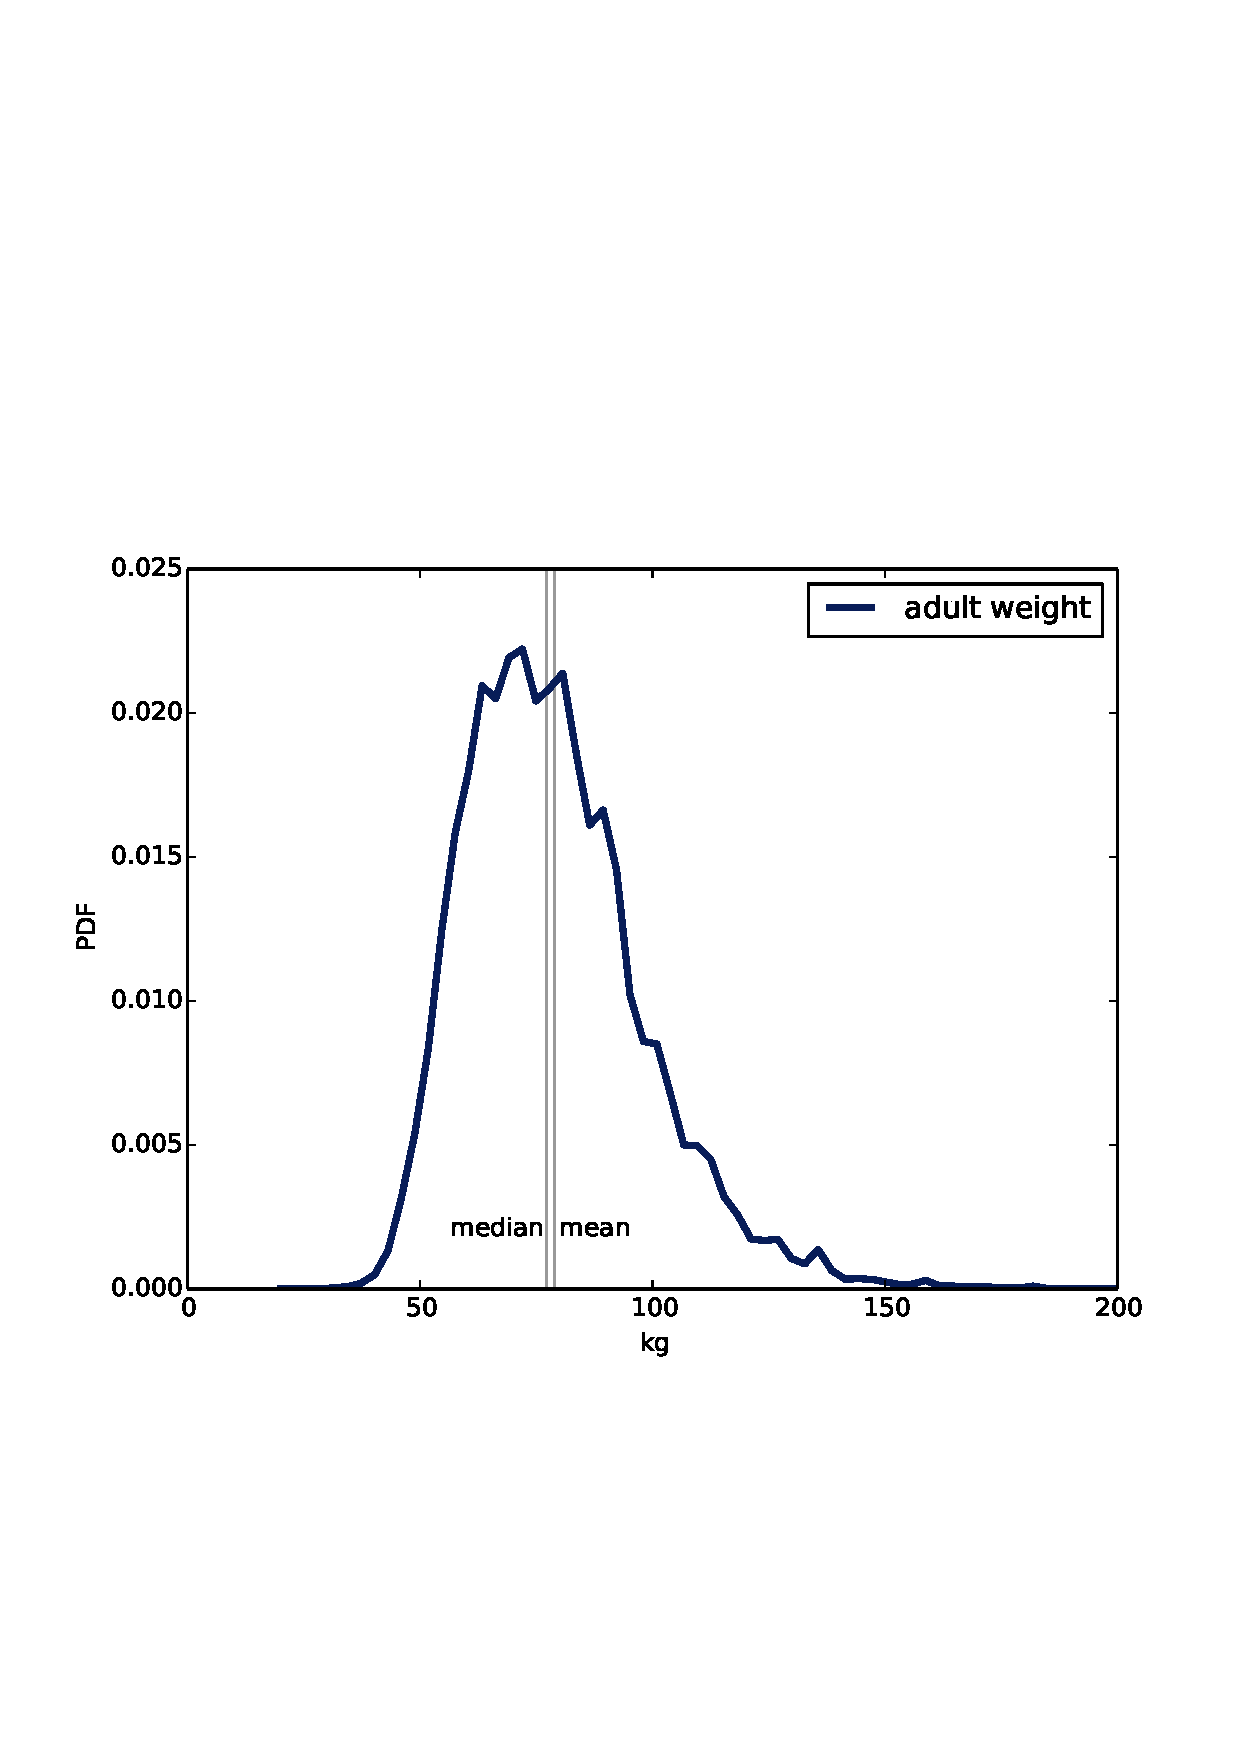
\includegraphics[height=2.2in]{figs/density_wtkg2_kde.pdf}}
\caption{BRFSS에서 나온 성인체중 데이터의 추정 PDF.}
\label{density_wtkg2_kde}
\end{figure}

이제 출생 체중 분포에 대해 BRFSS에 있는 성인 체중 분포와 비교해 보자.
다음에 파이썬 코드가 있다.
\index{thinkplot}

\begin{verbatim}
    df = brfss.ReadBrfss(nrows=None)
    data = df.wtkg2.dropna()
    pdf = thinkstats2.EstimatedPdf(data)
    thinkplot.Pdf(pdf, label='adult weight')
\end{verbatim}

그림~\ref{density_wtkg2_kde}에 결과가 있다.
분포가 오른쪽으로 기울어진 것으로 보인다.
말할 것도 없이, 평균이 79.0으로 중위수 77.3 보다 더 크다.
표본 왜도가 1.1이고 피어슨 중위수 왜도는 0.26이다.
\index{dropna}
\index{NaN}

왜도 계수 부호는 분포가 왼쪽 혹은 오른쪽으로 기울어진 것을 나타내지만,
그것을 제외하고 해석하기는 어렵다.
표본 왜도는 덜 강건하다; 즉, 특이점에 더 좌우된다.
결과로서 덜 믿음이 가는데, 기울어진 분포에 적용될 때, 정확하게 가장 관련될 때 그렇다. 

\index{특이점 (outlier)}
\index{강건성 (robust)}

피어슨 중위수 왜도는 계산된 평균과 분산에 기반한다.
그래서 특이점에 휘둘리기 쉽지만 제3 적률에 의존하지 않기 때문에 좀더 강건하다.
\index{피어스 중위수 왜도 (Pearson median skewness)}


\section{연습문제}

이 연습문제 해답은 \verb"chap06soln.py"에 나와있다.

\begin{exercise}

소득 분포는 유명하게도 우측으로 기울어져 있다.
이번 연습문제에서, 이 치우침이 얼마나 강한지 측정할 것이다.
\index{기울어짐}
\index{소득}

인구동향조사(Current Population Survey, CPS)는 노동통계국(Bureau of Labor Statistics)과 
인구조사국(Census Bureau)의 공동작업으로 소득과 관련된 변수를 연구한다.
2013년에 수집된 데이터는 \url{http://www.census.gov/hhes/www/cpstables/032013/hhinc/toc.htm}에서 다운로드 받을 수 있다.
저자는 가구소득 정보를 갖는 엑셀 파일 {\tt hinc06.xls} 을 다운로드 받아서,
이책의 저장소에서 찾을 수 있는 CSV 파일 {\tt hinc06.csv}로 변환했다.
이 CSV 파일을 불러읽는 {\tt hinc.py} 파일도 함께 있다.

\index{인구동향조사}
\index{노동통계국}
\index{인구조사국}

데이터셋은 소득구간과 해당 구간에 속하는 응답자수의 형태로 되어있다.
가장 낮은 구간은 ``\$5000 이하'' 이하 연간소득을 신고한 응답자가 포함된다.
가장 높은 구간은 ``\$250,000 이상'' 벌어들인 응답자가 포함된다.

이 데이터에서 평균과 다른 통계량을 추정하는데, 하한과 상한에 대해서, 그리고 각 구간에
값들이 어떻게 분포되었는지에 관해 가정을 해야한다.
{\tt hinc2.py} 파일에 {\tt InterpolateSample}이 제공되는데,
데이터를 모형화하는 한 방법을 보여주고 있다.
각 구간에 대한 상한을 담고 있는 {\tt income} 칼럼과 
각 구간에 응답자수를 담고 있는 {\tt freq} 칼럼을 갖는 데이터프레임을 인수로 받는다.
\index{데이터프레임}
\index{모형}

\verb"log_upper"도 인수로 받는데, {\tt log10} 달러로 표현되는 가장 소득이 높은 구간의 상한이다.
기본설정값 \verb"log_upper=6.0" 인데 응답자 가운데에 가장 높은 소득이 $10^6$, 즉 백만불이라는 
가정을 나타낸다.

{\tt InterpolateSample}는 유사표본을 생성한다; 즉,
각 구간에서 실제 데이터와 같은 응답자수를 산출해내는 가구소득 표본이다.
각 구간 소득이 log10 척도로 균등분할됨을 가정한다.

결과로 나온 표본에 대해 중위수, 평균, 기울어짐, 피어슨 기울어짐을 계산하시오.
평균이하 세금을 매길 수 있는 소득이 있는 가구 비율은 얼마인가?
결과가 가정한 상한에 얼마나 의존하는가?

\end{exercise}


\section{용어 사전}

\begin{itemize}

\item 확률밀도함수 (Probability density function, PDF): 
연속 CDF 미분으로 값을 확률 밀도에 매핑하는 함수.
\index{PDF}
\index{확률밀도함수 (probability density function)}

\item 확률밀도 (Probability density): 
  확률을 만들기 위해서 범위 값에 대해 적분할 수 있는 양.
  예를 들어, 만약 값 단위가 cm이라면, 확률밀도는 cm 당 확률 단위가 된다. 
\index{확률 밀도 (probability density)}

\item 핵밀도추정 (Kernel density estimation, KDE): 
  표본에 기반해서 PDF를 추정하는 알고리즘.
\index{핵밀도추정 (kernel density estimation)}
\index{KDE}

\item 이산화 (discretize): 
  연속함수 혹은 이산 함수를 가진 분포를 근사함. 평활(smoothing)의 반대.
\index{이산화 (discretize)}

\item 원적률 (raw moment): 
  거듭 제곱되는 데이터 합계에 기반한 통계량
\index{원적률 (raw moment)}

\item 중심적률 (central moment): 
  평균에서 편차 거듭제곱에 기반한 통계량.
\index{중심적률 (central moment)}

\item 표준적률 (standardized moment): 
  단위가 없는 적률 비율.
\index{표준적률 (standardized moment)}

\item 왜도 (skewness): 
  분포가 얼마나 비대칭인지 나타내는 측도.
\index{왜도 (skewness)}

\item 표본 왜도 (sample skewness): 
  분포 왜도를 정량화하는데 사용되는 적률기반 통계량.
\index{표본 왜도 (sample skewness)}

\item 피어슨 중위수 왜도 계수 (Pearson's median skewness coefficient): 
  중위수, 평균, 표준편차에 기반한 분포 왜도를 정량화하는데 사용되는 통계량.
  \index{피어슨 중위수 왜도 (Pearson median skewness)}

\item 강건성 (robust): 
  특이점에 상대적으로 면역되어 휘둘리지 않는다면 통계량은 강건하다.
\index{강건성 (robust)}

\end{itemize}




\chapter{변수간 관계}

지금까지 한번에 한 변수만 살펴봤다.
이번장에서 변수간 관계를 살펴본다.
변수 하나를 알고 있는 것이 다른 변수에 대한 정보를 준다면, 두 변수는 관계가 있다.
예를 들어, 신장과 체중은 관계가 있다; 키가 더 큰 사람이 체중이 더 나가는 경향이 있다.
물론, 완벽한 관계는 아니다: 키 작고 뚱뚱한 사람과 키 크고 마른 사람이 있다.
하지만, 다른 사람의 체중을 추측하려고 한다면, 신장 정보를 모르는 것보다 키 정보를 알고 있는 것이
좀더 정확하게 추정하는데 도움이 된다.

\index{성인 체중 (adult weight)}
\index{성인 신장 (adult height)}


이번 장에서 사용되는 코드는 {\tt scatter.py}에 있다.
코드를 다운로드하고 작업하는 것에 대한 정보는 ~\ref{code}을 참조한다.

\section{산점도 (Scatter plots)}
\index{산점도 (scatter plot)}
\index{그림 (plot)!산점도 (scatter)}

관계(relationship)을 확인하는 가장 간단한 방법이 {\bf 산점도 (scatter plot)}다.
하지만, 좋은 산점도를 만드는 것이 항상 쉬운 것은 아니다.
예제로, BRFSS 응답자에 대한 신장과 체중 플롯을 그릴 것이다. (~\ref{lognormal} 절 참조)
\index{BRFSS}

데이터 파일을 읽어서 신장과 체중 정보를 추출하는 코드가 다음에 있다.

\begin{verbatim}
    df = brfss.ReadBrfss(nrows=None)
    sample = thinkstats2.SampleRows(df, 5000)
    heights, weights = sample.htm3, sample.wtkg2
\end{verbatim}

{\tt SampleRows} 함수는 데이터에서 일부를 임으로 골라낸다. 
\index{SampleRows}

\begin{verbatim}
def SampleRows(df, nrows, replace=False):
    indices = np.random.choice(df.index, nrows, replace=replace)
    sample = df.loc[indices]
    return sample
\end{verbatim}

{\tt df}는 데이터프레임이고, {\tt nrows}는 선택할 행의 갯수가 되고, 
{\tt replace}는 복원 추출을 해야 하는지 나타내는 부울(boolean) 표식이다; 
다른 말로, 동일한 행이 한번 이상 선택되어 추출되는지 나타낸다. 

\index{데이터프레임 (DataFrame)}
\index{thinkplot}
\index{부울 (boolean)}
\index{복원 (replacement)}

{\tt thinkplot}에는 {\tt Scatter} 메쏘드가 있는데, 산점도를 그린다.
%
\begin{verbatim}
    thinkplot.Scatter(heights, weights)
    thinkplot.Show(xlabel='Height (cm)',
                   ylabel='Weight (kg)',
                   axis=[140, 210, 20, 200])
\end{verbatim}

그림~\ref{scatter1} (왼쪽)에 관계 형태를 보여주는 결과가 있다.
예상했던 것처럼, 더 키가 큰 사람이 더 체중이 나가는 경향이 있다.

\begin{figure}
% scatter.py
\centerline{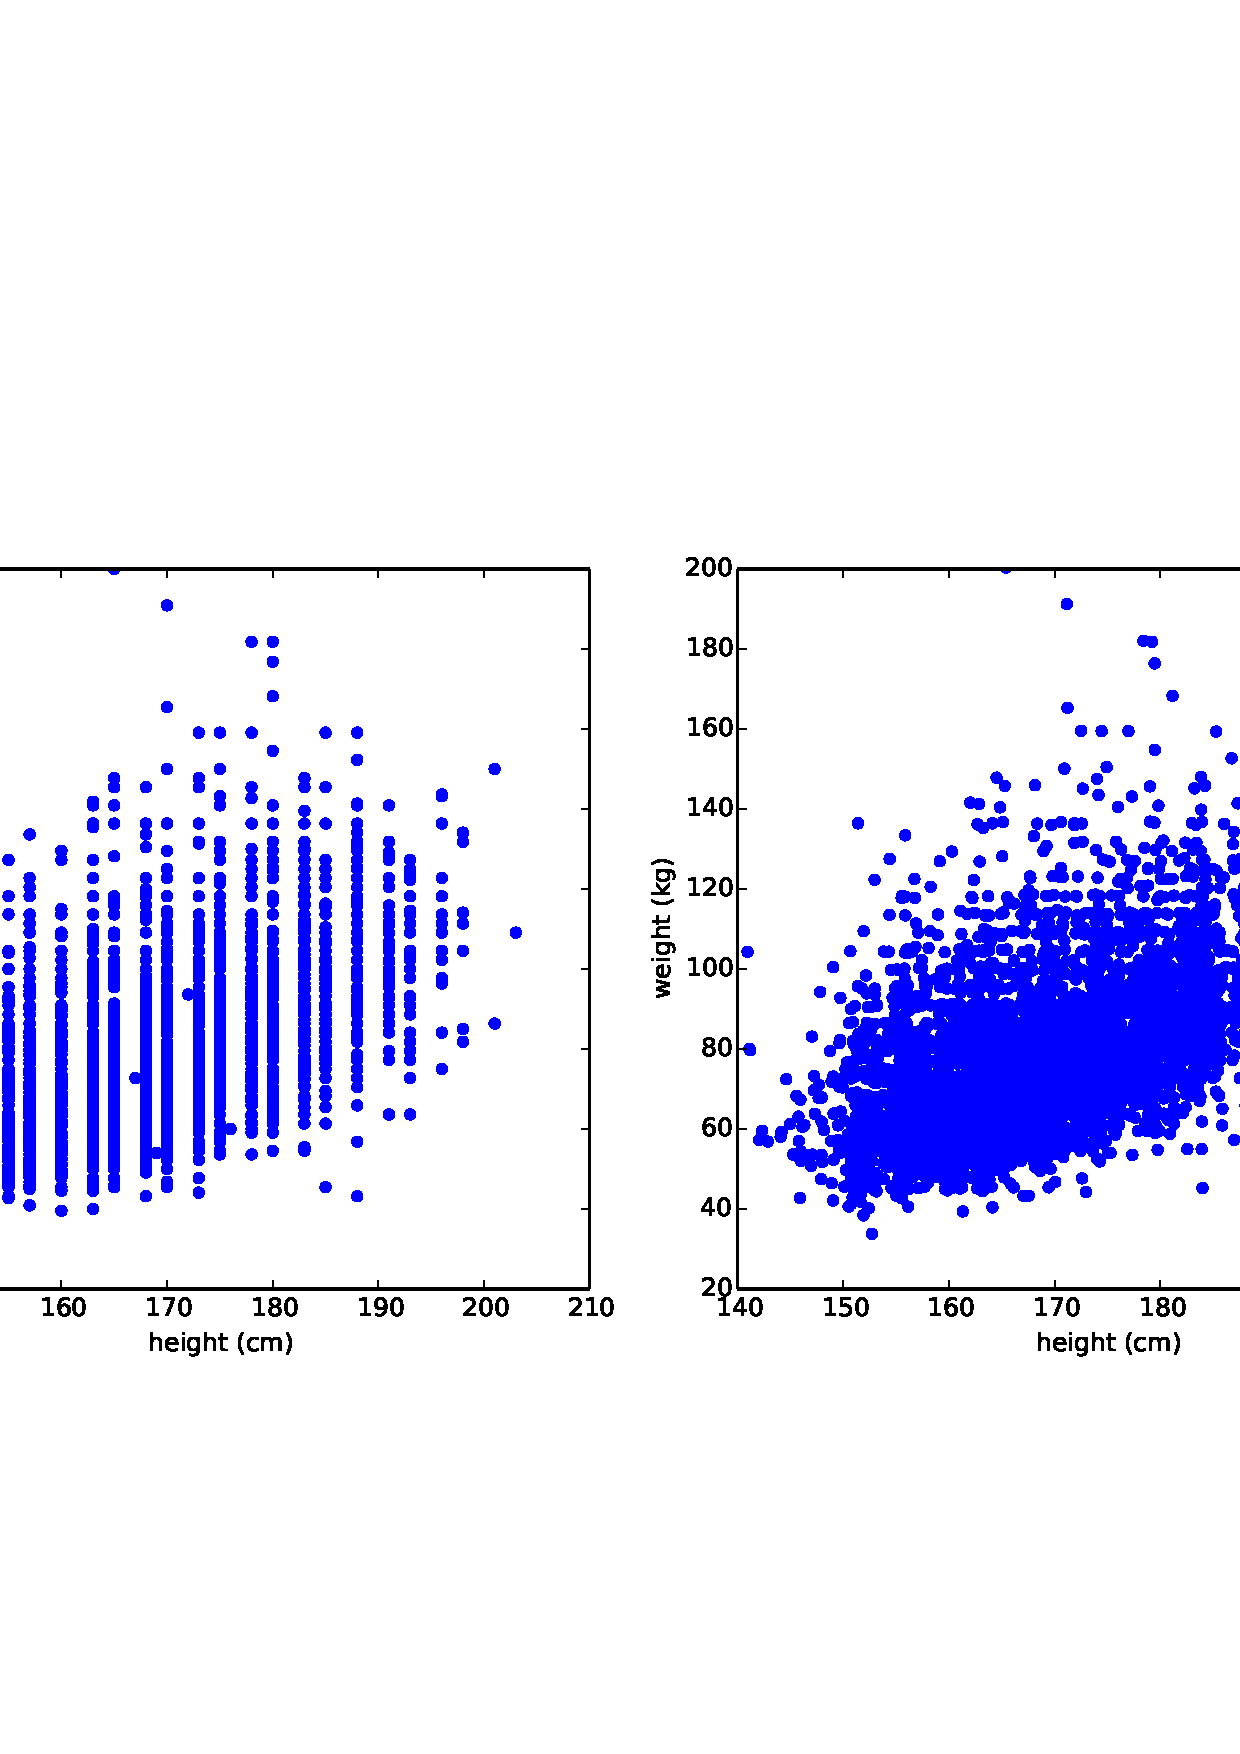
\includegraphics[height=3.0in]{figs/scatter1.pdf}}
\caption{지터되지 않은(좌측), 지터된(우측) 산점도로 BRFSS에서 응답자 신장과 체중을 도식화.}
\label{scatter1}
\end{figure}

하지만, 상기 그림이 데이터를 가장 잘 표현하는 것은 아니다.
이유는 데이터가 열에 떼지어 몰려있다. 문제는 
신장이 가장 가까운 인치(inch) 단위로 반올림되고, 센티미터로 변환하고 나서,
다시 반올림했다. 변환 과정에서 정보가 유실되었다.

\index{신장 (height)} 
\index{체중 (weight)} 
\index{지터 (jitter)}

유실된 정보를 다시 되돌릴 수는 없지만, 데이터를 {\bf 지터링(jittering)}\footnote{jittering, 지터로 번역을 했는데 통계 사전에는 등록이 되어있지 않고 일반 사전에는 ``조금씩 움직이다''라고 나와있다.}해서 
산점도에 효과를 최소화할 수 있다. 반올림 효과를 되돌리도록 확률 잡음(random noise)를 추가한다는 의미다.
측정값이 가장 근사한 인치(inch) 정보로 반올림되어 있어서, 0.5 인치 즉, 1.3 센티미터까지 차이가 생길 수도 있다. 마찬가지로, 체중은 0.5 kg까지 차이가 생길 수 있다. 

\index{균등 분포 (uniform distribution)}
\index{분포 (distribution)!균등 (uniform)}
\index{잡음 (noise)}

%
\begin{verbatim}
    heights = thinkstats2.Jitter(heights, 1.3)
    weights = thinkstats2.Jitter(weights, 0.5)
\end{verbatim}

{\tt Jitter} 함수를 구현한 것이 다음에 있다.

\begin{verbatim}
def Jitter(values, jitter=0.5):
    n = len(values)
    return np.random.uniform(-jitter, +jitter, n) + values
\end{verbatim}

값은 임의 시퀀스가 될 수 있다; 결과는 넘파이(NumPy) 배열이다.
\index{넘파이 (NumPy)}

그림~\ref{scatter1} (오른편)에 결과가 있다.
지터링(jittering)을 통해서 반올림으로 인한 시각적 효과를 줄이고,
관계 형태를 좀더 명확히 한다. 하지만, 일반적으로 시각화 목적으로만
데이터를 지터링해야 하고, 분석을 위해서 지터링된 데이터 사용은 피해야 한다.

지터링 조차도 데이터를 표현하는 가장 최선의 방법이 되지는 못한다.
중복되는 점이 많아서 그림에서 조밀한 부분에 있는 데이터를 숨기고,
균형이 맞지 않게 특이점을 강조한다. 이와 같은 효과를 {\bf 포화 (saturation)}라고 부른다.
\index{특이점 (outlier)}
\index{포화 (saturation)}

\begin{figure}
% scatter.py
\centerline{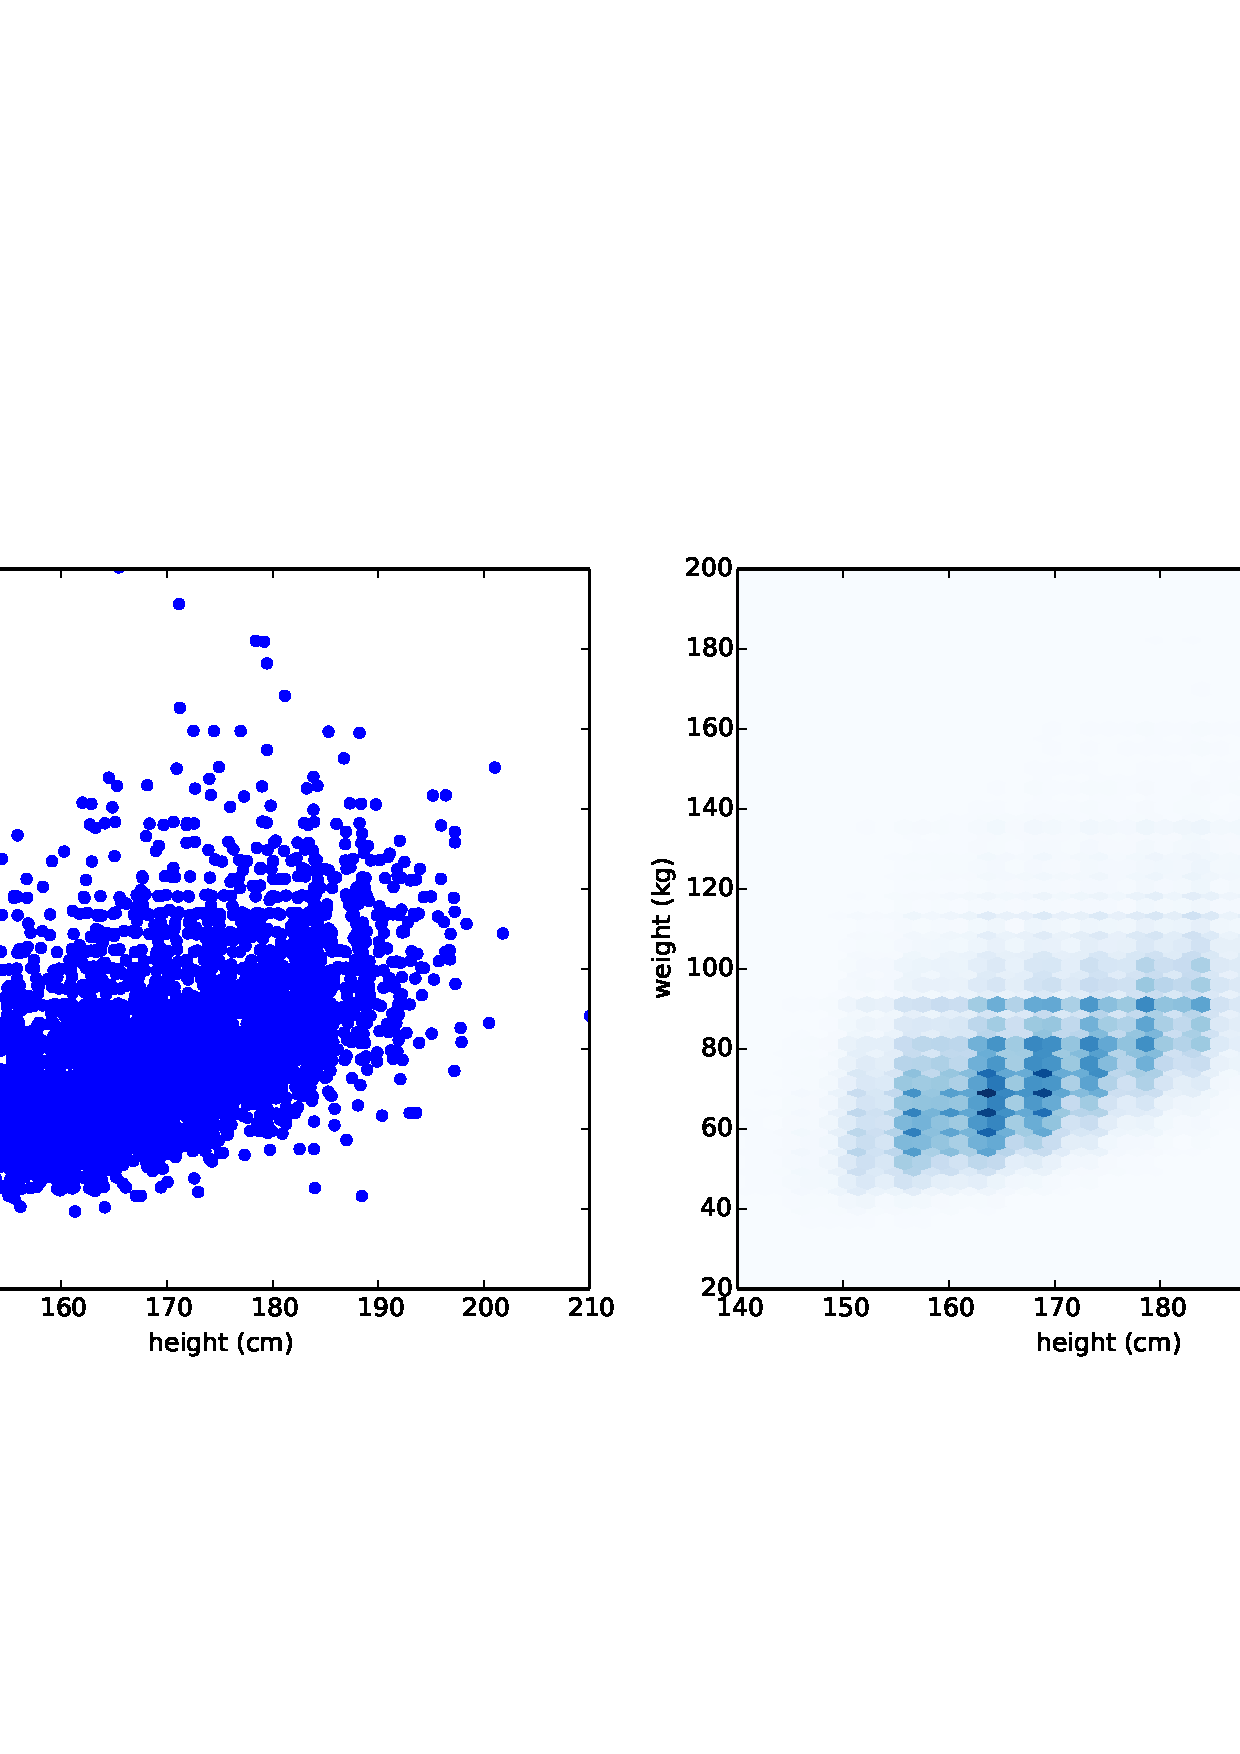
\includegraphics[height=3.0in]{figs/scatter2.pdf}}
\caption{지터되지 않은(좌측), 지터된(우측) 산점도로 BRFSS에서 응답자 신장과 체중을 도식화.}
\label{scatter2}
\end{figure}

이런 문제를 {\tt alpha} 모수로 해결할 수 있는데, 수행하는 역할은 점들을 부분적으로 투명하게 한다.

%
\begin{verbatim}
    thinkplot.Scatter(heights, weights, alpha=0.2)
\end{verbatim}
%

그림~\ref{scatter2} (왼편)에 결과가 있다.
겹쳐지는 데이터 점들이 더 어두워 보여서 색이 짙음이 밀도와 비례하여 균형을 맞춘다. 이 버젼으로 그린 플롯을 살펴보면, 앞에서 명확하지 않은 두가지 자세한 사항을 볼 수 있다; 90 kg 즉, 200 파운드 근처에 수평선과 몇군데 신장에서 수직 군집이 보인다. 데이터가 파운드 단위로 자기 응답에 기반하기 때문에, 가장 그럴듯한 설명은 응답자가 반올림한 값으로 보고를 한 것이다.

\index{thinkplot}
\index{alpha}
\index{투영성 (transparency)}

투명성을 사용해서 중간정도 크기 데이터셋를 처리했다.
하지만, 그림은 단지 BRFSS 자료 414 509 중에서 첫 5000 레코드만 보여준다.

\index{육각함 플롯 (hexbin plot)}
\index{플롯 (plot)!육각함 (hexbin)}

더 커다란 데이터셋을 처리하기 위한,
또 다른 선택지가 육각함 플롯 (hexbin plot)이 된다.
그래프를 육각형 통(hexagonal bin)으로 나누고 각 통을 얼마나 많은 데이터가 들어있는지에 따라 색을 칠한다. {\tt thinkplot}에 {\tt HexBin}메쏘드가 있다.
%
\begin{verbatim}
    thinkplot.HexBin(heights, weights)
\end{verbatim}
%

그림~\ref{scatter2} (오른편)에 결과가 있다.
육각함(hexbin)의 장점은 관계 형태도 보여준다는 것이고,
큰 데이터셋에 대해서도 시간과 파일 크기에 둘 관점에서 효율적이다.
단점은 특이점이 보이지 않는다는 것이다.
 
\index{thinkplot}
\index{특이점 (outlier)}

이 사례를 통해서 강조하고자 하는 것은 오해를 불러 일으키는 산출물 없이 관계를 명확하게 보여주는 산점도를 플롯으로 그리는 것이 쉬운 것은 아니라는 점이다.

\index{산출물 (artifact)}


\section{관계를 특징짓기}
\label{characterizing}

산점도는 변수 사이에 관계에 대한 일반적인 인상을 제공한다. 하지만, 관계 본질에 대한 더 많은 통찰을 주는 
다른 시각화방법이 있다. 한 선택지는 변수를 구간화(binning)하고 다른 변수 백분위수를 플롯으로 그리는 것이다.

\index{구간화 (binning)}

넘파이(NumPy)와 판다스가 데이터를 구간화하는 함수를 제공한다.
\index{넘파이 (NumPy)}
\index{판다스 (pandas)}

\begin{verbatim}
    df = df.dropna(subset=['htm3', 'wtkg2'])
    bins = np.arange(135, 210, 5)
    indices = np.digitize(df.htm3, bins)
    groups = df.groupby(indices)
\end{verbatim}

{\tt dropna} 메쏘드는 호명된 칼럼(열)에서 {\tt nan}가 있는 행을 제거한다. 
{\tt arange} 메쏘드는 135부터 210까지 (210은 포함하지 않고) 5만큼 증가하는 구간을 가진 넘파이 배열을 생성한다.

\index{dropna 메쏘드}
\index{digitize 메쏘드}
\index{NaN}

{\tt digitize} 메쏘드는 {\tt df.htm3}에 있는 각 값을 담고 있는 구간 인텍스를 계산한다.
결과는 정수 인텍스 넘파이(NumPy) 배열이다. 
가장 하위 구간에 속하는 값은 인덱스 0에 매핑된다. 가장 상위 구간에 속하는 값은 {\tt len(bins)}에 매핑된다.

\begin{figure}
% scatter.py
\centerline{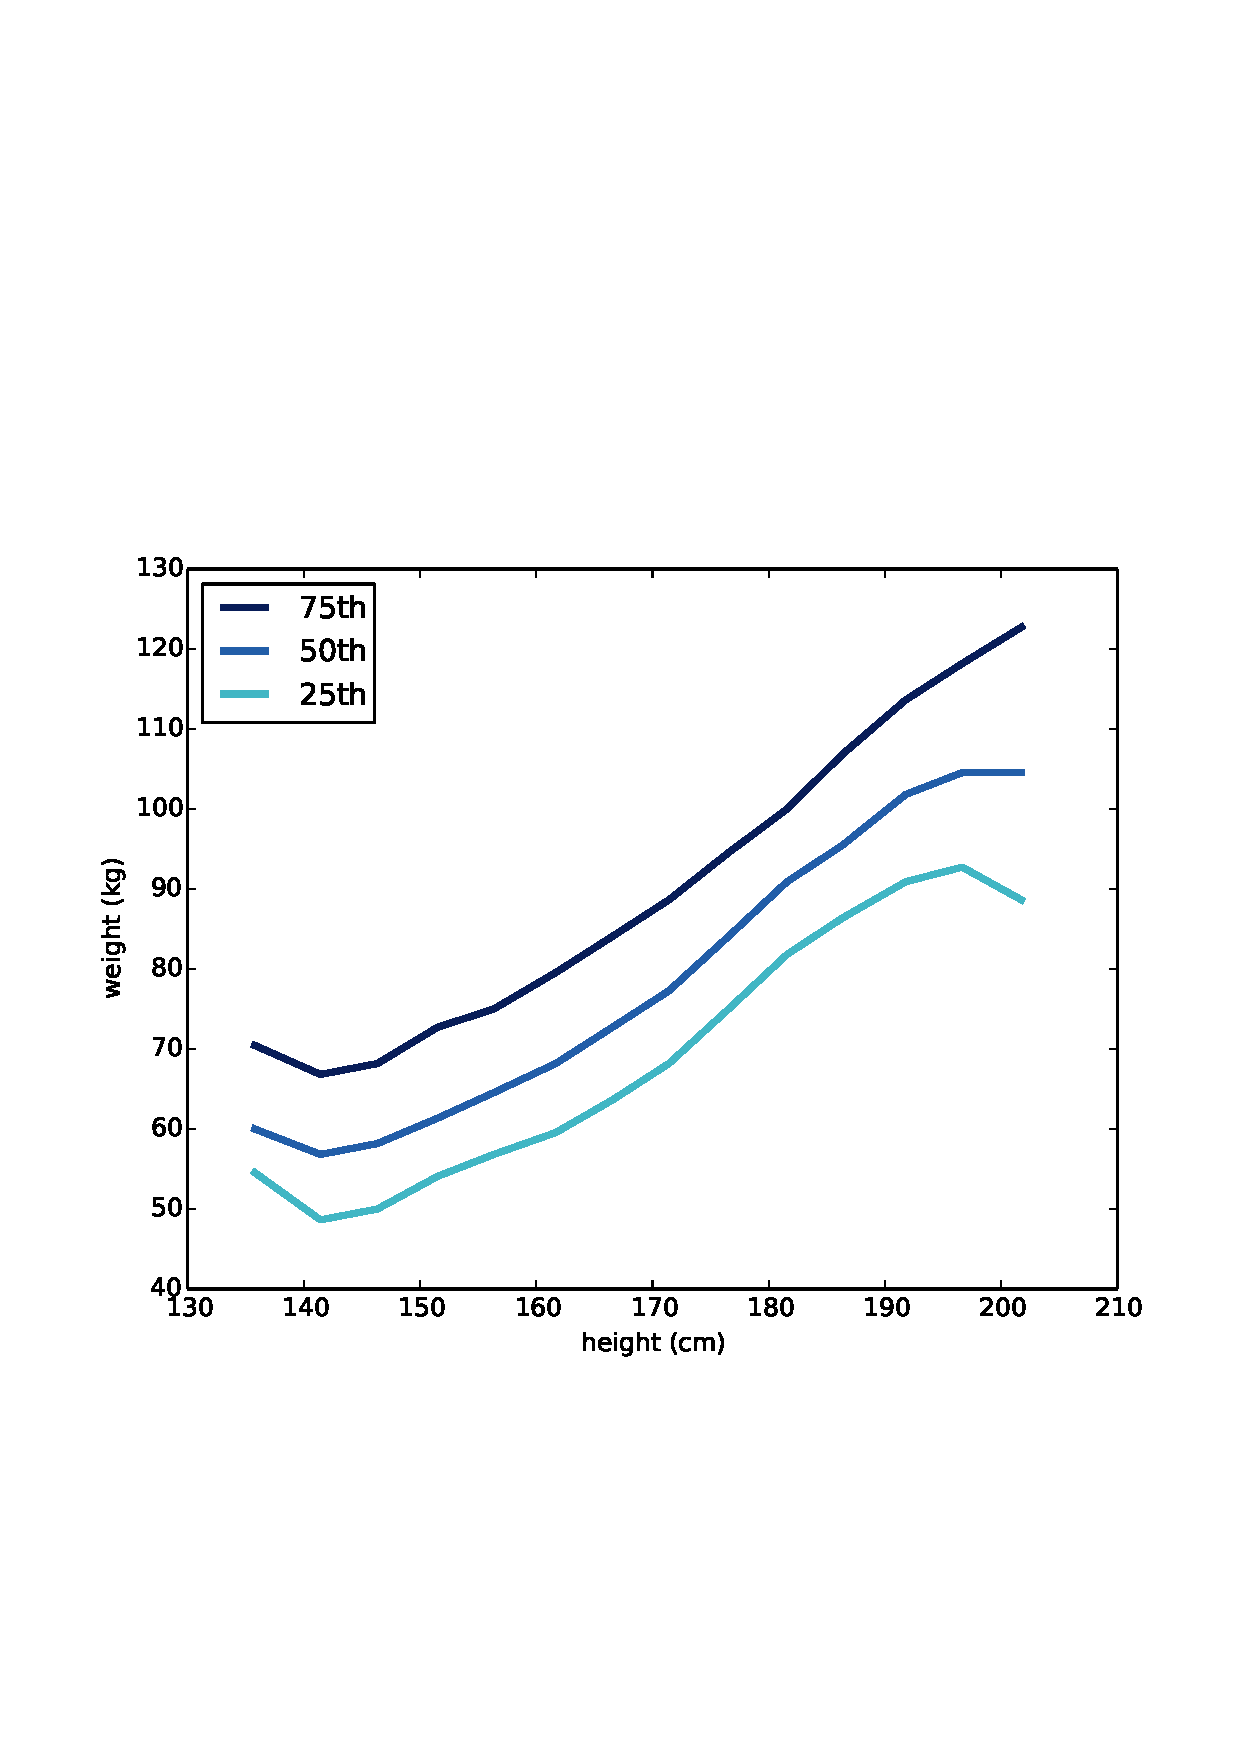
\includegraphics[height=2.5in]{figs/scatter3.pdf}}
\caption{신장 구간 범위에 대한 체중 백분위수.}
\label{scatter3}
\end{figure}

{\tt groupby}는 GroupBy 객체를 반환하는 데이터프레임 메쏘드다;
{\tt for} 루프에 사용되고, {\tt groups}은 그룹 이름과 그룹을 나타내는 데이터프레임을 반복돌린다.
\index{데이터프레임 (DataFrame)}
\index{groupby 메쏘드}

\begin{verbatim}
for i, group in groups:
    print(i, len(group))
\end{verbatim}

이제 각 그룹에 대해서, 평균 신장과 체중 CDF를 계산할 수 있다.
\index{Cdf}

\begin{verbatim}
    heights = [group.htm3.mean() for i, group in groups]
    cdfs = [thinkstats2.Cdf(group.wtkg2) for i, group in groups]
\end{verbatim}

마지막으로, 신장과 체중에 대한 백분위수를 플롯으로 그릴 수 있다.
\index{백분위수 (percentile)}

\begin{verbatim}
    for percent in [75, 50, 25]:
        weights = [cdf.Percentile(percent) for cdf in cdfs]
        label = '%dth' % percent
        thinkplot.Plot(heights, weights, label=label)
\end{verbatim}

그림~\ref{scatter3}에 결과가 나와 있다.
140센티미터에서 200센티미터 사이 두 변수 간의 관계는 대략 선형이다.
이 범위에 99\%이상 데이터가 몰려있다. 그래서, 극단값에 대해서 너무 걱정할 필요는 없다.
\index{thinkplot}


\section{상관 (Correlation)}

{\bf 상관 (correlation)}은 두 변수 간 관계강도를 정량화하는데 사용되는 통계량이다.
\index{상관 (correlation)}

상관을 측정하는데 걸림돌은 비교하려는 변수가 동일한 단위로 표현되지 않는다.
그리고 설사 단위가 동일하다고 하더라도, 다른 분포에서 두 변수가 나왔다.

\index{단위 (units)}

상기 문제에 대한 두가지 일반적인 해결책이 있다.

\begin{enumerate}

\item 각 값을 평균에서 떨어진 표준편차 숫자인 {\bf 표준점수 (standard scores)}로 변환한다. 
이러한 변환은 ``피어슨 곱적률 상관계수 (Pearson product-moment correlation coefficient)''가 된다.
\index{표준점수 (standard score)}
\index{표준편차 (standard deviation)}
\index{피어슨 상관계수 (Pearson coefficient of correlation)}

\item 각 값을 정렬된 리스트 값 인덱스인 {\bf 순위 (rank)}로 변환한다.
이러한 변환은 ``스피어만 순위 상관계수 (Spearman rank correlation coefficient)''가 된다.
\index{순위 (rank)}
\index{백분위수 순위 (percentile rank)}
\index{스피어만 상관계수 (Spearman coefficient of correlation)}

\end{enumerate}

만약 $X$가 일련 $n$개 값, $x_i$라면, 평균을 빼고 표준편차로 나누어서  
표준점수로 전환한다.
$z_i = (x_i - \mu) / \sigma$.
\index{평균 (mean)}
\index{표준편차 (standard deviation)}

분모가 편차다; 평균에서 떨어진 차이. $\sigma$로 나누면 편차를 {\bf 표준화(standardizes)}한다. 그래서 $Z$ 값은 차원이 없다(단위가 없음). 그리고 분포는 평균 0, 분산 1이 된다.
\index{표준화하다 (standardize)}
\index{차이 (deviation)}
\index{정규분포 (normal distribution)}
\index{분포 (distribution)!정규 (normal)}
\index{가우스 분포 (Gaussian distribution)}
\index{분포 (distribution)!가우스 (Gaussian)}

만약 $X$가 정규 분포라면, $Z$도 그렇다. 하지만, 만약 $X$가 기울어지거나 이상점이 있다면, $Z$도 그렇다; 이와 같은 경우, 백분위 순위를 사용하는 것이 좀더 강건하다.
만약 새로운 변수, $R$을 계산한다면, $r_i$는 $x_i$의 순위가 되고, $X$가 무슨 분포든지 관계없이, $R$ 분포는 1에서 $n$까지 균등분포다.

\index{균등분포 (uniform distribution)} 
\index{분포 (distribution)!균등 (uniform)}
\index{강건성 (robust)}
\index{왜도 (skewness)}
\index{이상점 (outlier)}


\section{공분산 (Covariance)}
\index{공분산 (covariance)}
\index{편차 (deviation)}

{\bf 공분산 (Covariance)}은 함께 변화하는 두 변수의 경향성 측도다.
만약 두 변수 계열 $X$ and $Y$가 있다면,
평균에 대한 편자는 다음과 같다.
%
\[ dx_i = x_i - \xbar \]
\[ dy_i = y_i - \ybar \]
%
$\xbar$가 $X$의 표본 평균이고, 
$\ybar$이 $Y$의 표본 평균이다.
만약 $X$와 $Y$가 함께 변한다면, 편차는 동일 기호를 갖는 경향이 있다.

두 변수를 함께 곱한다면, 곱이 양수가 될 때는 편차가 동일한 부호를 갖을 때고, 음수가 될 때는 반대 부호를 갖을 때다.
그래서, 곱을 합하게 되면 함께 변화하는 경향성 측도가 된다. 

공분산은 이들 곱의 평균이다.

%
\[ Cov(X,Y) = \frac{1}{n} \sum dx_i~dy_i \]
%
$n$은 두 계열 변수의 길이다. (두 계열 변수는 길이가 동일해야 한다.)

만약 선형대수학을 공부해따면, {\tt Cov}가 길이로 나눈 편차의 내적(dot product)이다. 그래서 만약 두 벡터가 동일하다면 공분산은 극대화되고, 직교(orthogonal)하면 0, 반대 방향으로 위치하면 부호가 음수가 된다. {\tt thinkstats2}는 {\tt np.dot}을 사용해서 {\tt Cov}를 효과적으로 구현한다.
\index{선형대수학 (linear algebra)}
\index{내적 (dot product)}
\index{직교 벡터 (orthogonal vector)}

\begin{verbatim}
def Cov(xs, ys, meanx=None, meany=None):
    xs = np.asarray(xs)
    ys = np.asarray(ys)

    if meanx is None:
        meanx = np.mean(xs)
    if meany is None:
        meany = np.mean(ys)

    cov = np.dot(xs-meanx, ys-meany) / len(xs)
    return cov
\end{verbatim}

초기 설정값으로 {\tt Cov}가 표본 평균에서 편차를 계산하거나 이미 계산된 평균값을 인자로 넘길 수 있다. 만약, {\tt xs}와 {\tt ys}이 파이썬 시퀀스라면, {\tt np.asarray}가 넘파이(NumPy) 배열로 전환한다.
만약 이미 넘파이(NumPy) 배열이라면, {\tt np.asarray}는 아무 것도 하지 않는다.

\index{넘파이 (NumPy)}

공분산 구현이 설명 목적으로 간단하게 구현되었다.
넘파이(NumPy)와 판다스에 공분산 구현되어 기능을 제공한다.
하지만, 둘다 여기서 다루어지지 않는 작은 표본 크기에 대한 보정기능을 제공한다. 그리고, {\tt np.cov}는 공분산 행렬을 반환하는데, 공분산 행렬은 지금 당장 필요한 것 이상이다.

\index{판다스 (pandas)}


\section{피어슨 상관 (Pearson's correlation)}
\index{상관 (correlation)}
\index{표준 점수 (standard score)}

공분산이 몇몇 연산에서는 유용하지만, 요약 통계량으로는 결코 보고되어지지 않는데 이유는 해석하기기 어렵기 때문이다.
다른 문제점 중에서, 단위가 $X$와 $Y$ 단위의 곱이다.
예를 들어, 이것이 무엇을 의미하든지, BRFSS 데이터셋에서 체중과 신장 공분산은 113 킬로그림-센티미터가 된다.

\index{편차 (deviation)}
\index{단위 (units)}

이 문제에 한 해결책은 표준편차로 편차를 나누고, 표준 점수 곱을 계산하는 것이다.

%
\[ p_i = \frac{(x_i - \xbar)}{S_X} \frac{(y_i - \ybar)}{S_Y} \]
%
$S_X$와 $S_Y$은 $X$와 $Y$의 표준편차다. 이들 곱의 평균은 다음과 같다.

%
\[ \rho = \frac{1}{n} \sum p_i \]
%
혹은 $S_X$ 와 $S_Y$을 빼내서 $\rho$를 다시 작성할 수 있다.
%
\[ \rho = \frac{Cov(X,Y)}{S_X S_Y} \]
%

이 값을 초창기 영향력 있는 통계학자 칼 피어슨(Karl Pearson)을 따라 {\bf 피어슨 상관 (Pearson's correlation)}이라고 부른다.
계산하기 쉽고 해석하기도 쉽다. 표준 점수는 차원이 없어서 $\rho$다.

\index{피어슨, 칼 (Pearson, Karl)}
\index{피어슨 상관계수 (Pearson coefficient of correlation)}

{\tt thinkstats2}에서 구현한 코드가 다음에 있다.

\begin{verbatim}
def Corr(xs, ys):
    xs = np.asarray(xs)
    ys = np.asarray(ys)

    meanx, varx = MeanVar(xs)
    meany, vary = MeanVar(ys)

    corr = Cov(xs, ys, meanx, meany) / math.sqrt(varx * vary)
    return corr
\end{verbatim}

별도로 {\tt np.mean}와 {\tt np.var}을 호출하기 보다 다소 더 효율적으로 {\tt MeanVar}은 평균과 분산을 계산한다.
\index{MeanVar}

피어슨 상관은 항상 -1과 1 사이다. (1,-1을 포함한다.) 만약, $\rho$가 양수라면, 상관이 양(positive)으로 한 변수값이 높으면, 다른 변수값도 높은 경향이 있다는 의미다. $\rho$가 부(negative)이면, 한 변수가값이 높으면, 다른 변수 값은 낮은 경향이 있다는 의미다.

$\rho$ 크기는 상관 강도를 나타낸다. 만약 $\rho$가 1 혹은 -1 이면, 변수는 완벽하게 상관되어 있다는 의미로, 만약 변수 하나를 알고 있다면 다른 하나에 대해서 완벽한 예측이 가능하다는 의미다.
\index{예측 (prediction)}

현실 세계에서 대부분의 상관은 완벽하지 않지만, 여전히 유용하다.
신장과 체중 상관은 0.51로 비슷한 사람과 관련된 변수와 비교하여 볼 때 강한 상관이다.

\section{비선형 관계 (Nonlinear relationships)}

만약 피어슨 상관이 거의 0이라면, 변수 사이에 관계가 없다고 단정하고 싶을 것이다. 하지만, 그러한 결론은 타당하지 않다. 피어슨 상관은 단지 {\em
  선형 (linear)} 관계만을 측정한다. 만약 비선형 관계가 있다면, $\rho$는 비선형 강도를 과소평가하게 된다.

\index{선형 관계 (linear relationship)}
\index{비선형 (nonlinear)}
\index{피어슨 상관 계수 (Pearson coefficient of correlation)}

\begin{figure}
\centerline{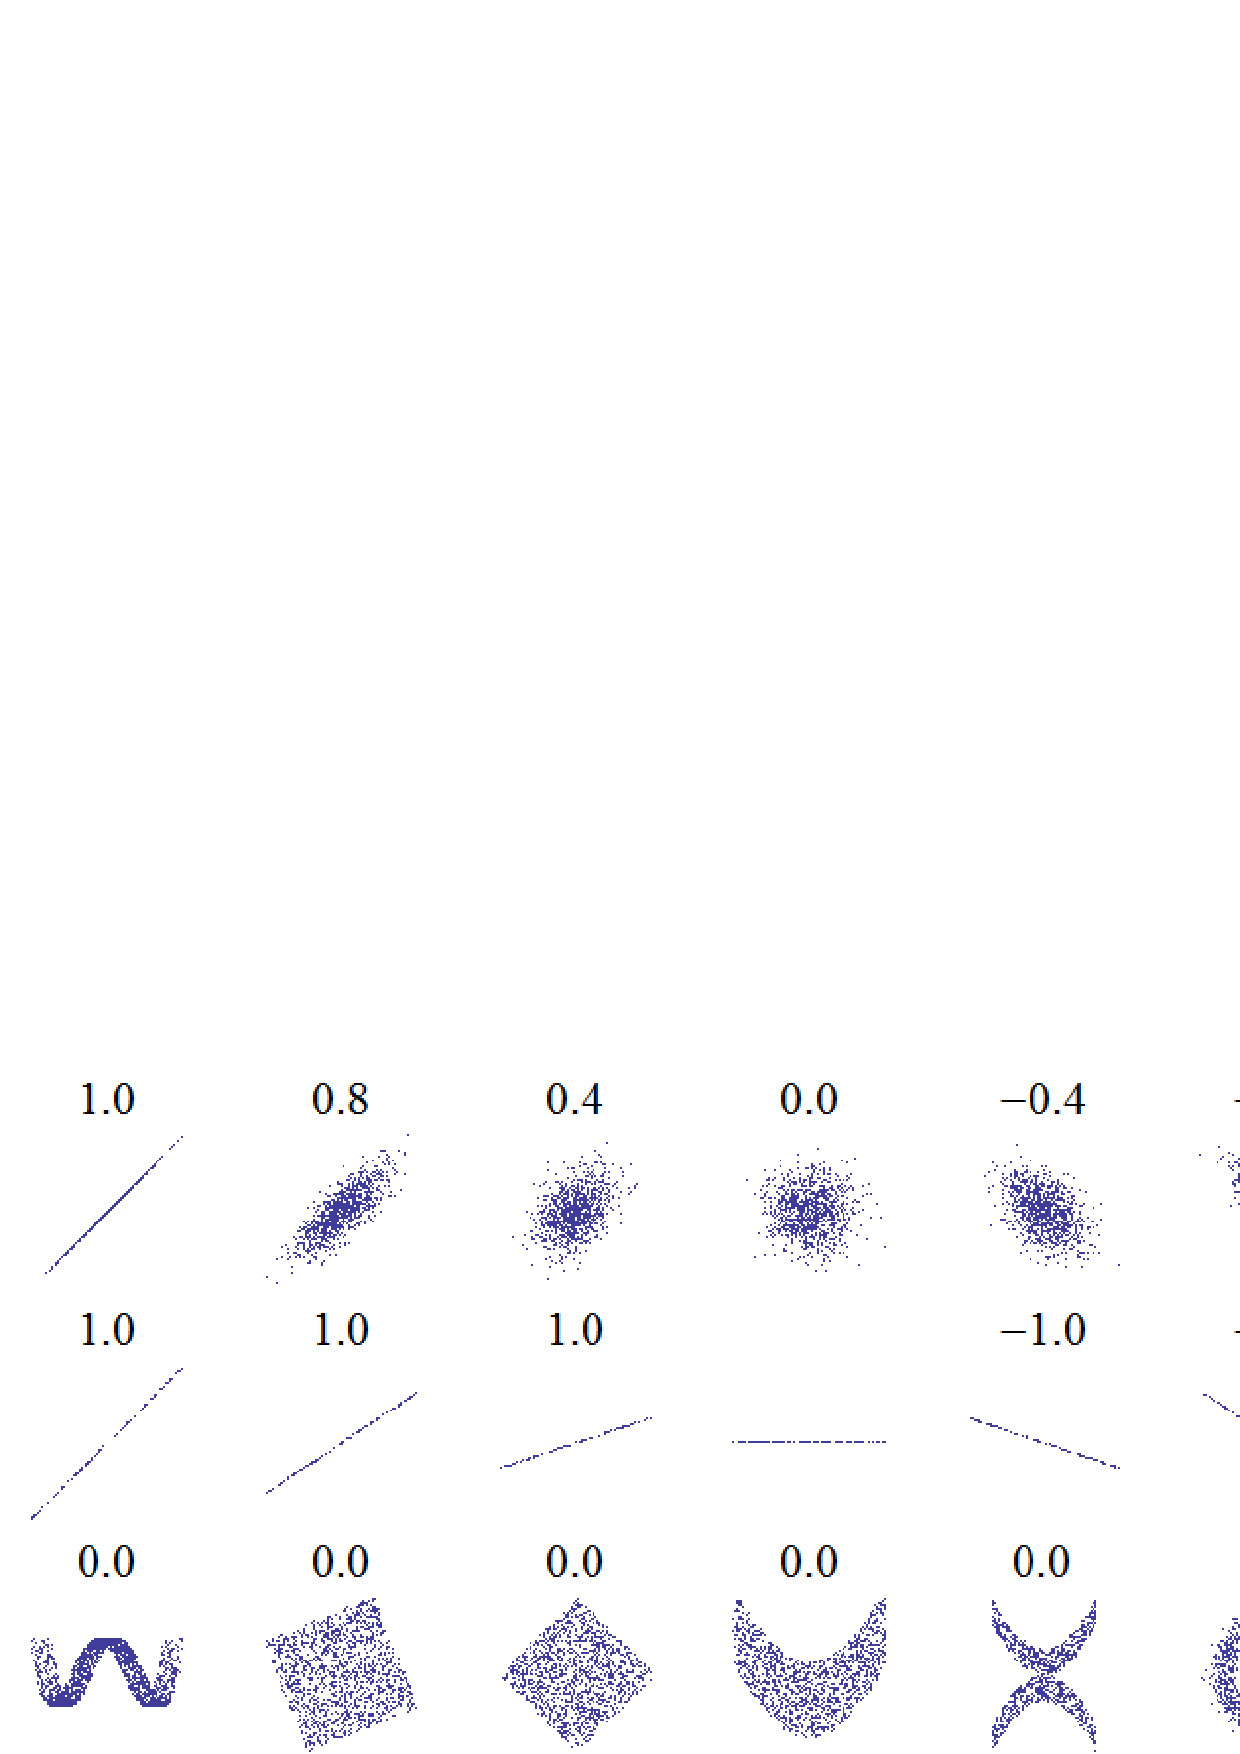
\includegraphics[height=2.5in]{figs/Correlation_examples.png}}
\caption{다양한 범위의 상관을 갖는 예제 데이터셋.}
\label{corr_examples}
\end{figure}

그림~\ref{corr_examples}은 \url{http://wikipedia.org/wiki/Correlation_and_dependence} 위키피디아 사이트에서 가져왔다.
그림에서 의도적으로 생성된 데이터셋에 대한 산점도와 상관 계수가 보여진다.
\index{산점도 (scatter plot)}
\index{그림 (plot)!산점 (scatter)}

상단 줄에는 다양한 상관계수를 가진 선형 관계를 보여준다; 상단 행에서 다양한 $\rho$ 값이 어떤 느낌인지 감을 얻을 수 있다.
두번째 행이 다양한 기울기를 가진 완전 상관의 예가 있다. 상관이 기울기와 관련이 없다는 것을 보여준다 (곧 기울기를 추정하는 것에 대해 언급할 것이다.) 세번째 행은 명확하게 관련이 있는 변수를 보여준다. 하지만, 관계가 비선형이라, 상관계수는 0이다.

\index{비선형 (nonlinear)}

상기 이야기의 교훈은 상관계수를 맹목적으로 계산하기 전에 데이터를 산점도를 그려서 항상 살펴봐야 한다는 것이다.

\index{상관 (correlation)}


\section{스피어만 순위 상관 (Spearman's rank correlation)}

피어슨 상관은 변수 사이의 관계가 선형이고, 변수가 대략 정규분포를 따른 다면 잘 동작한다. 하지만, 이상값이 존재하는 경우에는 강건하지 못하다.
스피어만 순위 상관이 대안으로 이상값과 기울어진 분포에 대한 효과를 완화한다. 
\index{피어슨 상관계수 (Pearson coefficient of correlation)}
\index{스피어만 상관계수 (Spearman coefficient of correlation)}
\index{정규분포 (normal distribution)}
\index{분포 (distribution)!정규 (normal)}
\index{가우스 분포 (Gaussian distribution)}
\index{분포 (distribution)!가우스 (Gaussian)}
\index{강건성 (robust)}
스피어만 상관을 계산하기 위해서 각 값의 {\bf 순위 (rank)}를 계산하는데 정렬된 표본에 인덱스에 해당한다.
예를 들어, 표본 {\tt [1, 2, 5, 7]}에서 값 5에 대한 순위는 3이다. 왜냐하면 정렬된 리스트에서 3번째 등장하기 때문이다. 그리고 나서 피어슨 순위 상관을 계산한다.

\index{왜도 (skewness)}
\index{이상값 (outlier)}
\index{순위 (rank)}

{\tt thinkstats2}는 스피어만 순위 상관을 계산하는 함수가 있다.

\begin{verbatim}
def SpearmanCorr(xs, ys):
    xranks = pandas.Series(xs).rank()
    yranks = pandas.Series(ys).rank()
    return Corr(xranks, yranks)
\end{verbatim}

인자를 판다스 시리즈 객체로 전환해서, 각 값에 대한 순위를 계산하고 시리즈를 반환하는 {\tt 순위 (rank)} 메쏘드를 사용할 수 있다. 
그리고 나서 {\tt Corr}을 사용해서 순위 상관을 계산한다.

\index{판다스 (pandas)}
\index{시리즈 (Series)}

직접적으로 {\tt Series.corr}을 사용해서 스피어만 메쏘드를 명세할 수도 있다.

\begin{verbatim}
def SpearmanCorr(xs, ys):
    xs = pandas.Series(xs)
    ys = pandas.Series(ys)
    return xs.corr(ys, method='spearman')
\end{verbatim}

BRFSS 데이터에 대한 스피어만 순위 상관계수는 0.54로 피어슨 상관계수 0.51보다 약간 더 높다. 차이에 대한 가능한 이유가 몇가지 있다:

\index{순위상관 (rank correlation)}
\index{BRFSS}

\begin{itemize}

\item 만약 관계가 비선형이면, 피어슨 상관은 관계의 강도를 과소추정하는 경향이 있다.
\index{비선형 (nonlinear)}

\item 만약 두 변수 분포중 하나가 기울거나(skewed) 이상점을 포함하게 되면, 피어슨 상관이 (어느 방향이든지) 영향을 받을 수 있다. 스피어만 상관계수가 좀더 강건하다.  

\index{기움 (skewness)}
\index{이상점 (outlier)}
\index{강건성 (robust)}

\end{itemize}

BRFSS 예제에서, 체중 분포가 대략 로그 정규분포라는 것을 알고 있다; 로그 변환을 통해서 정규 분포로 근사해서, 기울어짐이 없다.
기울어짐 효과를 제거하는 또다른 방법은 로그 취한 체중과 신장 사이 피어슨 상관을 계산하는 것이다.

\index{로그 정규분포 (lognormal distribution)}
\index{분포 (distribution)!로그 정규 (lognormal)}

\begin{verbatim}
    thinkstats2.Corr(df.htm3, np.log(df.wtkg2)))
\end{verbatim}

결과는 0.53으로 순위 상관계수 0.54에 가깝다. 그래서 이것이 의미하는 바는 체중 분포의 기울어짐이 피어슨과 스미어만 상관 사이 대부분 차이를 설명한다.
\index{기울어짐 (skewness)}
\index{스피어만 상관계수 (Spearman coefficient of correlation)}
\index{피어슨 상관계수 (Pearson coefficient of correlation)}


\section{상관과 인과 (Correlation and causation)}
\index{상관 (correlation)}
\index{인과 (causation)}

만약 변수 A와 B가 상관되었다면, 세가지 설명이 가능하다: A가 B의 발생 원인, B가 A의 발생 원인, 혹은 다른 요소가 A와 B의 발생 원인. 이와 같은 설명을 ``인과 관계 (causal relationships)''라고 부른다.
\index{인과 관계 (causal relationship)}

상관 그 자체로는 가능한 설명이 어느 것인지 구별하지는 못한다. 그래서, 어느 것이 사실인지 여러분에게 알려주지는 못한다. 이 원칙은 종종 다음 상용구로 표현된다. ``상관은 원인을 함축하지 않는다. (Correlation
does not imply causation)''.
애석하게도 자체 위키피디아 페이지도 있다. \url{http://wikipedia.org/wiki/Correlation_does_not_imply_causation}.

인과 증거를 제공하려면 무엇을 할 수 있을까요?

\begin{enumerate}

\item 시간을 사용한다. 만약 A가 B전에 온다면, A가 B를 발생시키는 원인 이지만, 다르게는 아니다. (적어도 인과에 관한 상식적인 이해에 따르면)
사건 순서는 인과 방향을 추론하는데 도움이 된다. 하지만, 다른 무언가 A와 B를 발생시키는 원인이 된다는 가능성을 배제하지 못한다.

\item 확률(randomness)을 사용한다. 만약 큰 표본을 임의로 두 집단으로 나누고 거의 모든 변수의 평균을 계산한다면, 차이는 작을 것으로 기대한다.
만약 한 변수를 제외하고 모든 변수에서 집단이 동일하다면, 허위 관계 (spurious relationship)을 제거할 수 있다.

\index{허위 관계 (spurious relationship)}

설사 관련 변수가 무엇인지 모른다고 하더라도 이 방식은 동작한다. 하지만, 관련 변수를 알고 있다면 더 잘 동작하는데 이유는 집단이 동일하다는 것을 확인할 수 있기 때문이다. 

\end{enumerate}

이와 같은 아이디어가 {\bf 무작위 대조군 시험 (randomized controlled
trial)}의 동기가 된다. 시험 대상이 임의로 두 (혹은 그 이상) 집단에 배속된다: {\bf 처리군 (treatment group)}은 신약 같은 일종의 개입을 받고, 
{\bf 대조군 (control group)}은 개입을 받지 않거나 효과가 알려진 또다른 처리를 받는다.

\index{무작위 대조군 시험 (randomized controlled trial)}
\index{대조군 시험 (controlled trial)}
\index{처리군 (treatment group)}
\index{대조군 (control group)}
\index{의학 (medicine)}

무작위 대조군 시험은 인과관계를 시연하는 가장 신뢰성 있는 방법이고, 과학-기반 의학의 초석이다. (\url{http://wikipedia.org/wiki/Randomized_controlled_trial} 참조).

불행하게도 대조군 시험은 실험실 과학, 의학, 그리고 몇몇 학문분야에서만 가능하다. 사회 과학에서, 대조군 실험이 드문데 이유는 불가능하거나 비윤리적이기 때문이다.
\index{윤리 (ethics)}

또 다른 대안은 {\bf 자연 실험 (natural experiment)}을 살펴보는 것인데, 다른 처리(treatment)가 유사한 집단에 적용된다. 자연 실험의 한가지 위험성은 명확하지 않는 방식으로 집단이 다를지도 모른다는 것이다.
이 주제에 대해서 웹사이트를 참조한다. \url{http://wikipedia.org/wiki/Natural_experiment}.
\index{자연 실험 (natural experiment)}

몇몇 경우에, {\bf 회귀 분석 (regression analysis)}을 사용해서 인과 관계를 추론할 수 있다. ~\ref{regression}장에서 다룰 것이다.
\index{회귀 분석 (regression analysis)}


\section{연습 문제}

이 연습문제 해답은 \verb"chap07soln.py"에 나와있다..

\begin{exercise}
NSFG 에서 나온 데이터를 사용해서,
출생체중과 산모연령 산점도를 그리시오.
출생체중과 산모연령 백분위수를 도식화하시오.
피어슨 상관과 스피어만 상관을 계산하시오.
두 번수 사이 관계를 어떻게 특징적으로 묘사할 수 있을까?
\index{출생체중}
\index{체중!출생}
\index{피어슨 상관계수}
\index{스피어만 상관계수}
\end{exercise}


\section{용어 사전}

\begin{itemize}

\item 산점도 (scatter plot): 두 변수 사이 관계를 데이터 각 행마다 점을 찍어 보임으로써 시각화.
\index{산점도 (scatter plot)}

\item 지터 (jitter): 시각화 목적으로 데이터에 추가되는 확률 잡음.
\index{지터 (jitter)}

\item 포화 (saturation): 다수의 점이 겹쳐지게 되어서 발생하는 정보 손실.
\index{포화 (saturation)}

\item 상관 (correlation): 두 변수 사이 관계 강도를 측정하는 통계량.
\index{상관 (correlation)}

\item 표준화(standardize): 변수 집합 값을 변환해서 평균 0, 분산 1로 만듦.
\index{표준화 (standardize)}

\item 표준 점수 (standard score): 표준화된 값으로, 평균에서 떨어진 표준편차로 표현.
\index{표준 점수 (standard score)}
\index{표준 편차 (standard deviation)}

\item 공분산 (covariance): 함께 변화하는 두 변수 경향성 측도.
\index{공분산 (covariance)}

\item 순위 (rank): 인덱스로, 정렬된 목록에 요소가 나타나는 순서.
\index{순위 (rank)}

\item 무작위 대조군 시험: 실험계획 (experimental design)으로 대상이 무작위 집단으로 나눠지고, 다른 집단에 다른 처리(treatment)가 주어진다.
\index{무작위 대조군 시험 (randomized controlled trial)}

\item 처리군 집단 (treatment group): 대조군 시험에서 일종의 개입(intervention)을 받는 집단.
\index{처리 집단 (treatment group)}

\item 대조군 집단 (control group): 대조군 시험에서 처리를 받지 않거나 이미 효과가 알려진 처리를 받는 집단.
\index{대조군 집단 (control group)}

\item 자연 실험 (natural experiment): 대상이 집단으로 자연 구분되는 현상을 이용하는 실험계획. 여기서 집단은 최소한 근사적으로 무작위가 된다.
\index{자연 실험 (natural experiment)}

\end{itemize}




\chapter{추정 (Estimation)}
\label{estimation}
\index{추정 (estimation)}

이번 장에서 사용되는 코드는 {\tt estimation.py}에 있다.
코드를 다운로드하고 작업하는 것에 대한 정보는 ~\ref{code}을 참조한다.


\section{추정 게임}

게임 한판합시다. 저자는 생각하는 분포가 있고, 여러분은 그 분포가 무엇인지 맞춰야 한다.
힌트를 두개 준다: 정규분포이고, 정규분포에서 나온 표본이 다음과 같다.

\index{정규분포 (normal distribution)}
\index{분포 (distribution)!정규 (normal)}
\index{가우스 분포 (Gaussian distribution)}
\index{분포 (distribution)!가우스 (Gaussian)}

{\tt [-0.441, 1.774, -0.101, -1.138, 2.975, -2.138]}

상기 분포의 평균 모수, $\mu$가 무얼까요?
\index{평균 (mean)}
\index{모수 (parameter)}

한가지 선택은 $\mu$ 추정값(estimate)으로 표본 평균 $\xbar$을 사용한다.
상기 예제애서 $\xbar$가 0.155 으로, $\mu$ = 0.155 추정하는 것은 합리적이다.
이러한 과정을 {\bf 추정 (estimation)}이라고 부른다. 사용한 통계량 (표본 평균)은 
{\bf 추정량(estimator)}이라고 부른다.
\index{추정량 (estimator)}

$\mu$를 추정하는데 표본 평균을 사용하는 것이 너무 명확해서 합리적인 다른 대안을 상상하기는 어렵다.
하지만, 이상값을 도입해서 게임을 바꾸는 것을 가정하자.
\index{정규분포 (normal distribution)}
\index{분포 (distribution)!정규 (normal)}
\index{가우스 분포 (Gaussian distribution)}
\index{분포 (distribution)!가우스 (Gaussian)}

{\em 저자가 생각하는 분포가 있다.} 정규분포이고, 잘못된 자리에 종종 소수점을 넣는
신뢰가 가지 않는 조사원이 수집한 표본이 다음에 있다.
\index{측정 오류 (measurement error)}

{\tt [-0.441, 1.774, -0.101, -1.138, 2.975, -213.8]}

이제 $\mu$ 추정값은 무엇이 될까요? 만약 표본 평균을 사용한다면, 추정치는 -35.12가 된다.
이것이 최선의 선택일까요? 대안이 무엇이 될까요?
\index{이상값 (outlier)}

한가지 선택지는 이상점을 식별하고 버리고 나서, 나머지를 가지고 표본 평균을 계산한다.
다른 선택지는 중위수를 추정량으로 사용한다.
\index{중위수 (median)}

어느 추정량이 가장 좋은가는 상황에 따라 달라지고(예를 들어, 이상값이 있느냐),
목적이 무엇이냐에 달려있다. 오류를 최소화하려고 하는지 혹은 정답을 얻는 가능성을 극대화하려고 하는지.

\index{오류 (error)}
\index{MSE}
\index{누적평균제곱오차 (mean squared error)}

만약 이상값이 없다면, 표본 평균은 {\bf 누적평균제곱오차 (mean squared
error), MSE}를 최소화한다. 즉, 만약 게임을 여러번하고, 매번 오차 
$\xbar - \mu$를 계산하면, 표본 평균은 다음을 최소화 한다.

%
\[ MSE = \frac{1}{m} \sum (\xbar - \mu)^2 \]
%
$m$은 추정 게임을 수행한 횟수다. $\xbar$를 계산하는데 사용된 표본 크기인 $n$와 혼동하면 안된다.

다음에 함수가 있는데 추정 게임을 모사하여 MSE 제곱근인, 
누적평균제곱오차의 제곱근(root mean squared error, RMSE)을 계산한다.

\index{누적평균제곱오차 (mean squared error)}
\index{MSE}
\index{RMSE}

\begin{verbatim}
def Estimate1(n=7, m=1000):
    mu = 0
    sigma = 1

    means = []
    medians = []
    for _ in range(m):
        xs = [random.gauss(mu, sigma) for i in range(n)]
        xbar = np.mean(xs)
        median = np.median(xs)
        means.append(xbar)
        medians.append(median)

    print('rmse xbar', RMSE(means, mu))
    print('rmse median', RMSE(medians, mu))
\end{verbatim}

다시 한번, {\tt n}은 표본 크기다. {\tt m}은 게임을 실행한 횟수다.
{\tt means}은 $\xbar$에 기반한 추정값 리스트다. 
{\tt medians}은 중위수 리스트다.
\index{중위수 (median)}

다음에 RMSE를 계산하는 함수가 있다.

\begin{verbatim}
def RMSE(estimates, actual):
    e2 = [(estimate-actual)**2 for estimate in estimates]
    mse = np.mean(e2)
    return math.sqrt(mse)
\end{verbatim}

{\tt estimates}는 추정값 리스트다; {\tt actual}은 추정되는 실제 값이다.
실무에서는 물론 {\tt actual}을 모른다; 만약 알고 있다면, 추정할 필요가 없을 것이다. 실험 목적은 두 추정량 성능을 비교하는 것이다.
\index{추정량 (estimator)}

코드를 실행하면, 표본 평균 RMSE가 0.41로 의미하는 바는 만약
$n=7$ 표본에 기반하여 $\xbar$를 사용해서 분포 평균을 추정한다면,
평균 0.41만큼 떨어졌다고 예측된다. 중위수를 사용하여 평균을 추정하면 RMSE 0.53을 산출하는데 적어도 이 사례에서 $\xbar$가 더 낮은 RMSE를 뽑아낸다고 확인해준다.

MSE 최소화는 좋은 특성이다. 하지만, 항상 최선의 전략은 되지 못한다.
예를 들어, 조선소에서 바람 속도 분포를 추정한다고 가정하다.
만약 추정값이 너무 높으면, 시설물을 과도하게 짓게되어서 비용이 상승한다.
하지만, 너무 낮게 추정한다면, 구조물이 붕괴할 수도 있다. 오류 함수로 비용이 좌우 대칭이 아니기 때문에, MSE 최소화가 항상 좋은 전략은 아니다.
\index{예측, (prediction)}
\index{비용 함수 (cost function)}
\index{MSE}

다른 예제로, 6면 주사위 세개를 던져서 합계를 예측하는 것을 가정하자.
정확하게 합계를 맞춘다면, 상을 받게 된다; 맞추지 못하면 아무 것도 없다.
이경우, MSE를 최소화하는 값은 10.5가 된다. 하지만, 좋지 못한 추정값이 된다.
왜냐하면 주사위 세개를 던져 합은 결코 10.5가 되지 못한다. 이 게임에서,
맞출 가장 높은 확률을 가진 추정량이 필요하다. 그것은 {\bf 최대우도추정량 (maximum likelihood estimator, MLE}이다. 만약 10 혹은 11일 선택하면,
우승 가능성이 8분의 1이 되고 할 수 있는 최선이 된다.

\index{MLE}
\index{최대우도추정량 (maximum likelihood estimator)}
\index{주사위 (dice)}


\section{분산 추정}
\index{분산 (variance)}
\index{정규분포 (normal distribution)}
\index{분포 (distribution)!정규 (normal)}
\index{가우스 분포 (Gaussian distribution)}
\index{분포 (distribution)!가우스 (Gaussian)}

{\em 저자가 마음에 두고 있는 분포가 있다.} 정규분포고, 다음에 (친숙한) 표본이 있다.

{\tt [-0.441, 1.774, -0.101, -1.138, 2.975, -2.138]}

상기 분포의 분산 $\sigma^2$가 무엇일까요? 다시 한번, 명백한 선택은
표본 분산, $S^2$를 추정량으로 사용하는 것이다.
%
\[ S^2 = \frac{1}{n} \sum (x_i - \xbar)^2 \] 
%

표본크기가 큰 경우, $S^2$가 적절한 추정량이 되지만, 작은 표본에 대해서 너무 작아지는 경향이 있다. 이와 같은 불행한 성질로 인해서, {\bf 편의 (biased)} 추정량이라고 부른다. 
만약 추정을 많이 반복한 뒤에 기대 총 (혹은 평균) 오류가 0이라면, 추정량은 
{\bf 불편의(unbiased)}다. 

\index{표본 분산 (sample variance)}
\index{편의 추정량 (biased estimator)}
\index{추정량 (estimator)!편의 (biased)}
\index{불편 추정량 (unbiased estimator)}
\index{추정량 (estimator)!불편 (unbiased)}

다행스럽게도, $\sigma^2$에 대한 불편 추정량인 또 다른 간단한 통계량이 있다.

%
\[ S_{n-1}^2 = \frac{1}{n-1} \sum (x_i - \xbar)^2 \] 
%

$S^2$가 왜 편의가 있고, $S_{n-1}^2$가 왜 불편 추정량인지에 대한 설명은 웹사이트 \url{http://wikipedia.org/wiki/Bias_of_an_estimator} 참조바랍니다.

이 추정량에 대한 가장 큰 문제점은 명칭과 기호가 일관되지 못하게 사용된다는데 있다. ``표본 분산''이 $S^2$ 혹은 $S_{n-1}^2$, 
그리고 기호 $S^2$이 한쪽 혹은 양쪽에 사용될 수 있다.

추정 게임을 모의시험하고 $S^2$ 와 $S_{n-1}^2$의 성능을 시험하는 함수가 다음에 있다.

\begin{verbatim}
def Estimate2(n=7, m=1000):
    mu = 0
    sigma = 1

    estimates1 = []
    estimates2 = []
    for _ in range(m):
        xs = [random.gauss(mu, sigma) for i in range(n)]
        biased = np.var(xs)
        unbiased = np.var(xs, ddof=1)
        estimates1.append(biased)
        estimates2.append(unbiased)

    print('mean error biased', MeanError(estimates1, sigma**2))
    print('mean error unbiased', MeanError(estimates2, sigma**2))
\end{verbatim}

한번 더, {\tt n}가 표본 크기이고, {\tt m}은 게임을 수행한 횟수다.
{\tt np.var}는 기본 설정으로 $S^2$을 계산하고, 만약 인자로 {\tt ddof=1}을 넣으면 $S_{n-1}^2$을 계산한다. {\tt ddof}는 ``델타 자유도 (delta degrees of freedom)''의 축약어다. 웹사이트에서 자세한 사항 참조한다. \url{http://en.wikipedia.org/wiki/Degrees_of_freedom_(statistics)}
\index{자유도 (degrees of freedom)}

{\tt MeanError}는 추정값과 실제값 사이 평균 차이를 계산한다.

\begin{verbatim}
def MeanError(estimates, actual):
    errors = [estimate-actual for estimate in estimates]
    return np.mean(errors)
\end{verbatim}

코드를 실행하면, $S^2$에 대한 평균 오차는 -0.13이다.
기대한 것처럼, 편의 추정량이 너무 적은 경향이 있다. 
$S_{n-1}^2$에 대해서, 평균 오차는 0.014로 10배 더 적다.
{\tt m}이 커감에 따라, 평균 오차 $S_{n-1}^2$가 0에 수렴해간다.

\index{평균 오차 (mean error)}

MSE나 편의(bias) 같은 성질은 많은 추정 게임에 기반한 장기 기대가 된다.
이장에서와 같은 모의시험을 수행해서, 추정량을 비교하고, 바람직한 성질을 갖는지 점검할 수 있다.

\index{편의 추정량 (biased estimator)}
\index{추정량 (estimator)!편의 (biased)}

하지만, 추정량을 실제 데이터에 적용했을 때,
단지 하나 추정값만 얻는다. 추정값이 편의가 없다고 말하는 것이 의미가 없을 수 있다; 불편(unbiased)하다는 것은 추정량(estimator)의 성질이지 추정값(estimate)의 성질은 아니다.

적절한 성질을 갖는 추정량을 선택하고 추정값을 생성하고 나면, 다음 단계는 추정값의 불확실을 특성화해야 한다. 다음 절의 주제다.


\section{표집 분포 (Sampling distributions)}
\label{gorilla}

야생동물 보호구역에서 고릴라를 연구하고 있는 과학자를 가정해보자.
보호구역에 서식하고 있는 성인 암컷 고릴라 평균 체중을 알고자 한다.
체중을 측정하려고 한다면, 고릴라를 진정시켜야 하는데, 위험하고, 비용이 많이 들며, 아마도 고릴라 자체도 해로울 수 있다.
하지만, 체중 정보 수집이 중요하다면, 9마리 고릴라를 표본으로 체중을 측정하는 것은 용인될지 모른다.
보호구역 모집단은 알고 있다고 가정하자. 그래서 성인 암컷 대표 표본을 고를 수 있다. 미지의 모집단 평균 $\mu$를 추정하는데 표본 평균 $\xbar$를 사용할 수 있다.
\index{고릴라 (gorilla)}
\index{모집단 (population)}
\index{표본 (sample)}

고릴라 암컷 9마리 체중을 재서, 표본평균 $\xbar=90$ kg과 표본 표준편차 $S=7.5$ kg을 찾았다. 
표본평균은 $\mu$에 대한 불편 추정량이고, 장기적으로 MSE를 최소화한다. 그래서 결과를 요약하는 단 하나 추정값을 보고한다면, 90 kg을 보고할 것이다.
\index{MSE}
\index{표본평균 (sample mean)}
\index{편의 추정량 (biased estimator)}
\index{추정량 (estimator)!편의 (biased)}
\index{표준편차 (standard deviation)}

하지만, 이 추정값에 대해서 얼마나 신뢰를 가져야할까?
훨씬 더 큰 모집단에서 단지 $n=9$ 마리 고릴라만 체중을 측정했다면, 우연히도 운이 좋지 못하다면 가장 무거운 (혹은 가장 가벼운) 고릴라만 고를 수 있다.
확률 선택(random selection)에 의해서 발생되는 추정값의 변동을 {\bf 표집 오차 (sampling error)}라고 한다.
\index{표집 오차 (sampling error)}

표집 오차를 정량화하기 위해서, 가설(hypothetical) 값 $\mu$와 $\sigma$를 갖는 표본추출 과정을 모의시험하고, $\xbar$가 얼마나 변화하는지 살펴볼 수 있다.

모집단 $\mu$와 $\sigma$ 실제값을 모르기 때문에, 
$\xbar$와 $S$을 추정값으로 사용한다. 
그래서 정답을 찾고 있는 질문은
``만약 $\mu$와 $\sigma$의 실제값이 90 kg와 7.5 kg이고,
동일한 실험을 많이 수행한다면, 추정된 평균 $\xbar$가 얼마나 변화할까요?''

다음 함수가 질문에 답을 한다.

\begin{verbatim}
def SimulateSample(mu=90, sigma=7.5, n=9, m=1000):
    means = []
    for j in range(m):
        xs = np.random.normal(mu, sigma, n)
        xbar = np.mean(xs)
        means.append(xbar)

    cdf = thinkstats2.Cdf(means)
    ci = cdf.Percentile(5), cdf.Percentile(95)
    stderr = RMSE(means, mu)
\end{verbatim}

{\tt mu}와 {\tt sigma}는 모수에 대한 {\em 가설 (hypothetical)} 값이다.
{\tt n}이 표본 크기로 체중을 측정한 고릴라 숫자다.
{\tt m}은 모의 시험을 수행한 횟수다.
\index{고릴라 (gorilla)}
\index{표본 크기 (sample size)}
\index{모의시험 (simulation)}

\begin{figure}
% estimation.py
\centerline{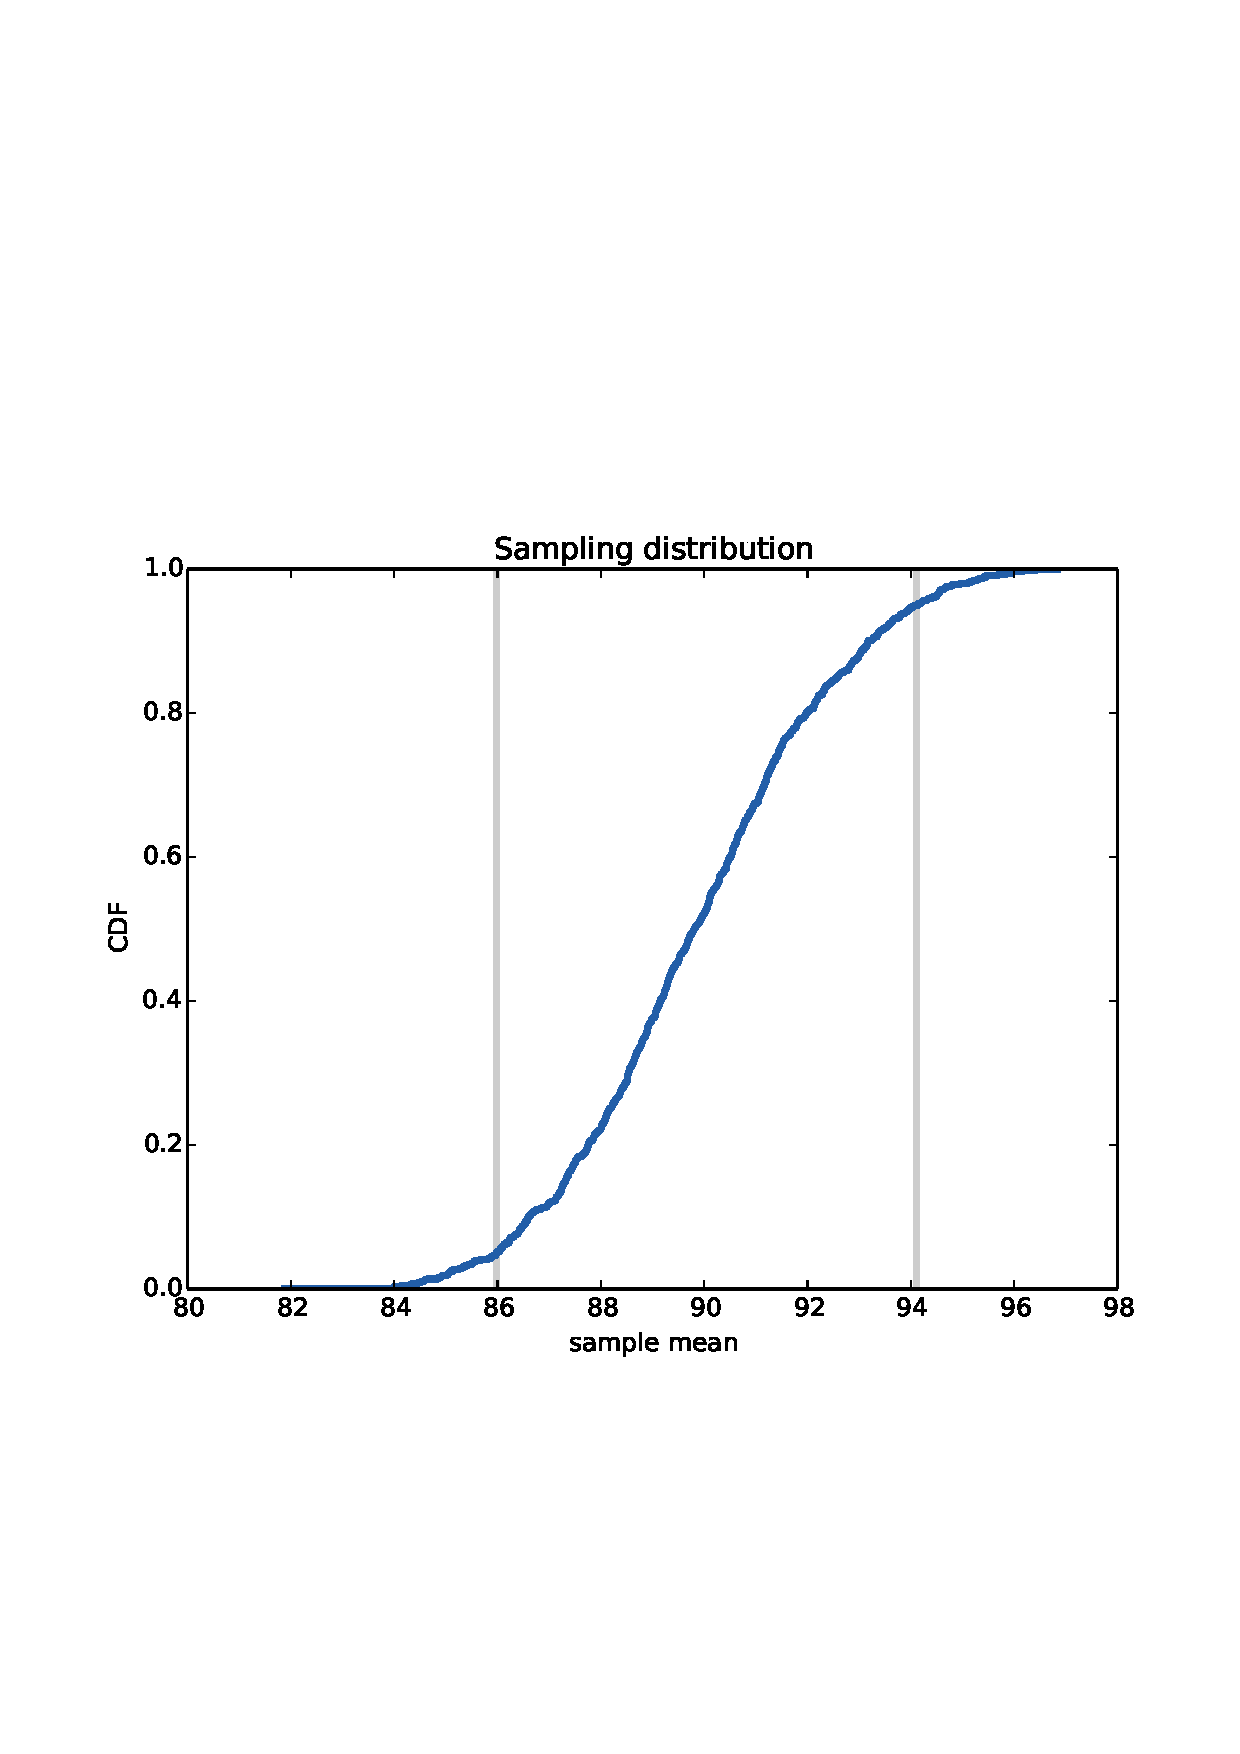
\includegraphics[height=2.5in]{figs/estimation1.pdf}}
\caption{신뢰구간과, $\xbar$ 표집분포.}
\label{estimation1}
\end{figure}

매번 반복할 때마다, 주어진 모수를 가진 정규분포에서 {\tt n}개 값을 골라 
표본 평균 {\tt xbar}를 계산한다. 1000번 모의시험하고 나서, 추정값 분포 {\tt cdf}를 계산한다. 결과가 그림 ~\ref{estimation1}에 나타나 있다.
분포를 추정값의 {\bf 표집 분포 (sampling distribution)}라고 부른다.
만약 반복해서 실험을 계속한다면, 추정값이 얼마나 변화하는지 보여준다.
\index{표집 분포 (sampling distribution)}

표집 분포 평균이 가정값(hypothetical value) $\mu$와 매우 가깝다.
따라서, 평균적으로 실험이 정답을 산출한다는 의미다.
1000회 반복한 후에는 가장 적은 값이 82 kg, 가장 큰 값이 98 kg이다.
이 범위가 함의하는 바는 추정값이 8 kg 만큼 차이가 있을 수 있다는 것이다.

표집 분포를 요약하는 두 가지 흔한 방법이 있다.

\begin{itemize}

\item {\bf 표준 오차 (Standard error SE)}는 평균적으로 추정값이 얼마나 차이가 있을지 측정하는 측도다. 각 모의 실험마다, 오차 $\xbar - \mu$를 계산하고 나서 누적평균제곱오차에 제곱근(root mean squared error, RMSE)을 씌워 계산한다. 상기 예제에서는 대략 2.5 kg이 된다.
\index{표준 오차 (standard error)}

\item {\bf 신뢰 구간 (confidence interval, CI)}은 표집 분포를 주어진 비율로 포함할 범위가 된다. 예를 들어, 신뢰 구간 90\%는 5번째부터 95번째 백분위수 범위가 된다. 상기 예제에서, 90\% CI는 $(86, 94)$ kg가 된다.
\index{신뢰 구간 (confidence interval)}
\index{표집 분포 (sampling distribution)}

\end{itemize}

표준 오차와 신뢰구간은 또한 혼동의 원천이기도 하다.

\begin{itemize}

\item 종종 표준 오차(standard error)와 표준편차(standard deviation)를 혼동한다. 표준 편차는 측정량에 내재한 변동성을 기술한다; 상기 예제에서, 고릴라 체중의 표준 편차는 7.5 kg이다. 표준 오차는 추정값에 내재한 변동성을 기술한다. 상기 예제에서, 표본 9 측정에 기반한 평균의 표준 오차는 2.5 kg 이다.

\index{고릴라 (gorilla)}
\index{표준 편차 (standard deviation)}

차이점을 기억하는 방법은, 표본 크기가 증가함에 따라, 
표준 오차는 점점 더 작아진다; 표준 편차는 그렇지 않다.
  
\item 90\% 확률로 실제 모수 $\mu$가 90\% 신뢰구간 내에 속한다고 생각하곤 한다. 슬프게도, 이것은 사실이 아니다.
이와 같은 주장을 하려고 한다면, 베이즈 방법(Bayesian method)을 사용해야 한다.(원저작자 책, {\it Think Bayes}을 참조).
\index{베이즈 통계 (Bayesian statistics)}

표집 분포는 다른 질문에 대한 답이다; 만약 실험을 반복한다면, 추정값이 얼마나 변화할 것인지 정보를 제시함으로써 추정값이 얼마나 신뢰할만한지 정보를 제공한다.
\index{표집 분포 (sampling distribution)}

\end{itemize}

신뢰 구간과 표준 오차는 표집 오차만 정량화한다는 것을 기억하는 것이 중요하다; 즉, 모집단 일부만 측정함으로써 생기는 오차.
표집 분포가 다른 오차를 설명하지는 않는다.
다른 오차는 표집 편의(sampling bias)와 측정 오차 (measurement error)가 포함되고 다음 절의 주제다. 

\section{표집 편의 (Sampling bias)}

자연보호구역에 고릴라 체중 대신에, 도시에 거주하고 있는 여성 평균 체중을 알고자 한다고 가정하자. 여성 대표 표본을 골라 체중을 측정하는 허가가 날 것 같지는 않다.

\index{고릴라 (gorilla)}
\index{성인 체중 (adult weight)}
\index{표집 편의 (sampling bias)}
\index{편의 (bias)!표집 (sampling)}
\index{측정 오차 (measurement error)}

간단한 대안은 ``전화 표집 (telephone sampling)''이 될 것이다; 
즉, 전화번호부에서 임의 번호를 골라, 전화하고, 성인 여성과 통화하여, 체중이 얼마인지 조사하는 것이다. 

\index{전화 표집 (telephone sampling)}
\index{난수 (random number)}

전화 표집은 분명한 한계가 있다.
예를 들어, 표본이 전화번호가 전화번호부에 등재된 사람으로 국한된다.
그래서 전화가 없는 사람(평균보다 더 가난할지 모르는 사람)과 전화번호부에 등재되지 않은 사람(훨씬 더 부자일 수 있는 사람)은 제외된다. 
또한, 낮 시간에 집으로 전화를 걸게 되면, 직장을 가진 사람이 표본에 있을 가능성은 줄어든다. 그리고 만약 전화에 응답한 사람만 표본으로 추출한다면, 전화를 공용으로 사용하는 사람을 표본으로 덜 추출할 것 같다.

수입, 실업, 가구 규모 같은 요인이 체중과 관련이 있다면(관련이 있을 듯하다.), 조사 결과가 어떻게든지 영향을 받을 수 있다. 이러한 문제를 {\bf 표집 편의 (sampling bias)}라고 부른다. 왜냐하면 표집과정(sampling process)의 한 특성이기 때문이다.
\index{표집 편의 (sampling bias)}

이러한 표집 과정은 또한 자기 선택(self-selection)에 취약한데 일종의 표집 편의다.
일부 사람은 질문에 대답을 거부한다. 그리고 만약 거부하는 경향이 체중과 관련된다면, 결과에도 영향을 줄 수 있다.
\index{자기 선택 (self-selection)}

마지막으로, 체중을 측정하기보다, 체중이 얼마인지 설문한다면, 결과가 정확하지 않을 수도 있다.
만약 실제 본인 체중에 불편하다면, 심지어 도움되는 응답자 조차도 체중을 올리거나 내릴지도 모른다. 그리고 모든 응답자가 도움이 되는 것은 아니다.
이와 같은 비정확성이 {\bf 측정 오차 (measurement error)} 사례가 된다.
\index{측정 오차 (measurement error)}

추정량을 보고할 때, 표집 오차를 정량화하기 위해서 표준 오차 혹은 신뢰구간, 혹은 모두 보고하는 것이 유용한다.
하지만, 표집 오차는 단지 오차의 단지 하나일 뿐이고, 종종 가장 큰 것이 아니라는 것을 기억하는 것이 중요하다.
\index{표준 오차 (standard error)}
\index{신뢰구간 (confidence interval)}


\section{지수분포 (Exponential distributions)}
\index{지수분포 (exponential distribution)}
\index{분포 (distribution)!지수 (exponential)}

한번더 추정 게임을 시도해보자. 
{\em 저자가 마음속에 분포를 하나 염두에 두고 있다.}
지수분포로, 다음에 표본이 있다.

{\tt [5.384, 4.493, 19.198, 2.790, 6.122, 12.844]}

상기 분포 모수 $\lambda$는 무엇이라고 생각하나요?

\index{모수 (parameter)}
\index{평균 (mean)}

\newcommand{\lamhat}{L}
\newcommand{\lamhatmed}{L_m}

일반적으로 지수분포 평균은 $1/\lambda$다. 그래서 역산해서 다음을 선택할 수 있다.
%
\[ \lamhat = 1 / \xbar\]
%
$\lamhat$은 $\lambda$의 추정량이다. 그리고 보통 다른 추정량과 다르다; 또한 최우추정량(maximum likelihood estimator)이다. (\url{http://wikipedia.org/wiki/Exponential_distribution#Maximum_likelihood} 참조).
그래서, 만약 정확하게 $\lambda$ 추측 확률을 극대화하려고 한다면, $\lamhat$이 나갈 방향이 된다.
\index{MLE}
\index{최우추정량 (maximum likelihood estimator)}

하지만, $\xbar$가 이상점이 존재하는 경우 강건하지 않다는 것을 알고 있다.
그래서, $\lamhat$도 동일한 문제를 작고 있다고 예상한다.
\index{강건성 (robust)}
\index{이상값 (outlier0}
\index{표본 중위수 (sample median)}

표본 중위수에 기반한 대안을 선택할 수 있다.
지수 분포 중위수는 $\ln(2) / \lambda$이다. 
다시 역산해서 계산하면, 추정량을 다음과 같이 정의한다.
%
\[ \lamhatmed = \ln(2) / m \]
%
여기서, $m$은 표본 중위수다.
\index{중위수 (median)}

이들 추정량 성능을 시험하기 위해서, 표집 과정을 모의 시험할 수 있다.

\begin{verbatim}
def Estimate3(n=7, m=1000):
    lam = 2

    means = []
    medians = []
    for _ in range(m):
        xs = np.random.exponential(1.0/lam, n)
        L = 1 / np.mean(xs)
        Lm = math.log(2) / thinkstats2.Median(xs)
        means.append(L)
        medians.append(Lm)

    print('rmse L', RMSE(means, lam))
    print('rmse Lm', RMSE(medians, lam))
    print('mean error L', MeanError(means, lam))
    print('mean error Lm', MeanError(medians, lam))
\end{verbatim}

$\lambda=2$로 실험을 하면, $L$ RMSE는 1.1 이 된다.
중위수 기반 추정량 $L_m$, RMSE는 1.8 이 된다.
실험으로부터 $L$ 이 MSE를 최소화했는지 분간할 수 없다.
하지만 적어도 $L_m$ 보다 더 좋은 듯 하다.
\index{MSE}
\index{RMSE}

슬프게도 두 추정량 모두 편의가 있다. $L$에 대해 평균 오차는 0.33; 
$L_m$에 대해 평균 오차는 0.45 다. 그리고 어느 것도 {\tt m}이 증가함에 따라 0 으로 수렴하지 않는다.
\index{편의 추정량 (biased estimator)}
\index{추정량 (estimator)!편의 (biased)}

$\xbar$는 분포 평균의 불편 추정량 $1 / \lambda$임이 밝혀졌다. 하지만,
$L$은 $\lambda$의 불편 추정량은 아니다.

\section{연습문제}

다음 연습문제에 대해서, {\tt estimation.py}을 복사해서 시작할 수 있다.
해답은 \verb"chap08soln.py" 파일에 나와있다.

\begin{exercise}

이번 장에서, $\mu$를 추정하는데 $\xbar$ 와 중위수를 사용했고,
$\xbar$가 MSE 하한을 산출함을 알아냈다.
또한, $\sigma$를 추정하는데 $S^2$ 와 $S_{n-1}^2$을 사용했고,
$S^2$은 편향되었고, $S_{n-1}^2$은 불편향임을 알아냈다.

유사한 실험을 실행해서, $\xbar$와 중위수가 $\mu$의 편향된 추정값임을 알아내라.
또한, $S^2$ 혹은 $S_{n-1}^2$ 가 MSE 하한을 산출하는지 검사하라.

\index{표본 평균}
\index{표본 중위수}
\index{추정량!편향된}

\end{exercise}


\begin{exercise}

모수 $\lambda=2$를 갖는 지수분포에서 표본 $n=10$ 개를 추출한다고 가정하자.
실험을 1000번 모의시험하고 추정값 $\lamhat$의 표본 분포를 도식화한다.
추정값의 표준오차와 90\% 신뢰구간을 계산하라.

\index{표준오차}
\index{신뢰구간}
\index{표본분포}

다른 $n$ 값을 갖는 실험을 반복하고, $n$ 값과 표준오차를 도식화한다.
\index{지수분포}
\index{분포!지수}


\end{exercise}


\begin{exercise}

하키와 축구같은 스포츠 게임에서 득점 사이 시간은 대체로 지수를 따른다.
그래서 게임에서 한 팀이 득점한 골을 관측함으로써 득점을 추정할 수 있다.
이 추정 과정은 득점 사이 시간을 표집하는 것과 약간 다르다. 
그래서 작동방법을 살펴보다.

\index{하키}
\index{축구}

게임당 골로 득점률 {\tt lam}을 인자로 받고,
전체 시간이 1 게임 경과할 때까지 득점사이 시간을 생성함으로서 게임을 
모의시험하고 나서, 득점한 점수를 반환하는 함수를 작성하라. 

많은 게임을 모의시험하고, {\tt lam} 추정값을 저장하고 나서
평균 오차와 RMSE를 계산하는 또다른 함수를 작성하라.

추정값을 이와 같은 방식으로 만드는 것이 편향됐을까?
추정값에 대한 표본분포와 90\% 신뢰구간을 도식화하시오.
표준오차는 얼마인가? 
{\tt lam} 값을 크게하면, 표집오차에 무슨일이 생길까?

\index{추정량!편향된}
\index{편향된 추정량}
\index{표준오차}
\index{신뢰구간}

\end{exercise}


\section{용어 사전}

\begin{itemize}

\item 추정 (estimation): 표본에서 분포 모수를 추정하는 과정.
\index{추정 (estimation)}

\item 추정량 (estimator): 모수를 추정하는데 사용되는 통계량.
\index{추정량 (estimator)}

\item 누적평균제곱오차 (mean squared error, MSE): 추정 오차 측도.
\index{누적평균제곱오차 (mean squared error)}
\index{MSE}

\item 제곱근 평균제곱오차 (root mean squared error, RMSE): 
MSE 제곱근으로 일반적인 오차 규모를 좀더 유의미하게 표현.
\index{누적평균제곱오차 (root mean squared error)}
\index{RMSE}

\item 최우추정량 (maximum likelihood estimator, MLE): 가장 올바를 것 같은 점추정값을 계산하는 추정량.
\index{MLE}
\index{최우추정량 (maximum likelihood estimator)}

\item (추정량의) 편의 (bias of an estimator): 반복되는 실험을 평균낼 때, 실제 모수 값보다 높은 혹은 낮은 추정량의 경향성. 
\index{편의 추정량 (biased estimator)}

\item 표집 오차 (sampling error): 
우연에 의한 변동과 한정된 표본 크기 때문에 추정값에 생기는 오차.
\index{점추정 (point estimation)}

\item 표집 편의 (sampling bias): 
모집단을 대표하지 못하는 표집 과정 때문에 추정값에 생기는 오차.
\index{표집 편의 (sampling bias)}

\item 측정 오차 (measurement error): 
데이터를 수집하고 기록하는 부정확성 때문에 추정값에 생기는 오차.
\index{측정 오차 (measurement error)}

\item 표집 분포 (sampling distribution): 
만약 실험을 많이 반복한다면 생기는 통계량 분포.
\index{표집 분포 (sampling distribution)}

\item 표본 오차 (standard error): 
추정값의 RMSE로 표집 오차 (하지만 다른 오차는 제외) 때문에 생기는 변동성을 정량화한다.
\index{표본 오차 (standard error)}

\item 신뢰구간 (confidence interval): 
만약 실험을 많이 반복하면 추정량 예상 범위를 표현하는 구간.
\index{신뢰구간 (confidence interval)} 
\index{구간 (interval)!신뢰 (confidence)}

\end{itemize}



\chapter{가설 검정 (Hypothesis testing)}
\label{testing}

이번 장에서 사용되는 코드는 {\tt hypothesis.py}에 있다.
코드를 다운로드하고 작업하는 것에 대한 정보는 ~\ref{code}을 참조한다.


\section{전통적 가설 검정 (Classical hypothesis testing)}
\index{가설 검정 (hypothesis testing)}
\index{외관 효과 (apparent effect)}

NSFG에서 데이터를 탐색하면서, 첫째 아이와 첫째가 아닌 아이들 간 차이를 
포함해서 몇가지 ``외관 효과 (apparent effects)''를 봤다.
지금까지 액면 그대로 이러한 효과를 받아들였다; 이번 장에서 이를 검정한다. 

\index{국가 가정 성장 조사 (National Survey of Family Growth)}
\index{NSFG}

다루고자 하는 근본적인 질문은 표본에서 본 효과가 더 큰 모집단에서 나타날 것인가다.
예를 들어, NSFG 표본에서 첫째 아이와 첫째 아이가 아닌 아이들에 대한 평균 임신 기간에
차이를 봤다. 알고자 하는 것은 이 효과가 미국 여성에 대한 진정한 차이를 반영하는지 
혹은, 우연히 표본에서 생겨난 것이냐다.
\index{임신 기간 (pregnancy length)} 
\index{기간 (length)!임신 (pregnancy)}

피셔 귀무 가설 검정(Fisher null hypothesis testing), 네이만 피어슨 의사결정 이론(Neyman-Pearson decision theory), 베이즈 추론(Bayesian inference)\footnote{베이즈 추론에 대한 좀더 많은 정보는 후속해서 출간되는 {\it Think Bayes}를 참조한다.}을 포함해서 질문을 구성하는 방법이 몇가지 있다.
여기 제시하는 것은 대부분의 사람이 실무에서 사용하는 세가지 방법의 일부분으로 {\bf 전통적 가설 검정 (classical hypothesis testing)}이라고 저자가 작명한 것이다.
\index{베이즈 추론 (Bayesian inference)}
\index{귀무 가설 (null hypothesis)}

전통적 가설 검정의 목적은 다음 질문에 답하는 것이다.
``표본과 명백한 효과가 주어졌다면, 우연히 그런 효과를 목도하는 확률이 얼마인가?''
다음에 질문에 답을 하는 방법이 있다.

\begin{itemize}

\item 첫번째 단계는 {\bf 검정 통계량 (test statistic)}을 선택해서 
외관 효과 크기를 정량화한다. NSFG 예제에서, 명백한 효과는 첫번째 아이와 첫째가 아닌 아이들 사이에 임신 기간에 차이가 된다. 그래서, 검정 통계량에 대한 자연스러운 선택이
두 집단 사이에 평균 차이가 된다.
  \index{검정 통계량 (test statistic)}

\item 두번째 단계는 {\bf 귀무 가설 (null hypothesis)}을 정의하는 것으로,
명백한 효과가 사실이 아니라는 가정에 기반한 시스템 모형이다.
NSFG 예제에서, 귀무 가설은 첫째 아이와 첫째가 아닌 아이들 사이에 차이가 없다가 된다;
즉, 두 집단 임신 기간은 동일한 분포다. 
\index{귀무 가설 (null hypothesis)}
\index{임신 기간 (pregnancy length)}
\index{모형 (model)}

\item 세번째 단계는 {\bf p-값(p-value)}을 계산하는 것으로, 만약 귀무 가설이 사실이라면 명백한 효과를 볼 확률값이 된다. NSFG 예제에서, 평균에 실제 차이를 계산하고 나서, 귀무 가설 아래에서 차이를 크게 혹은 더 크게 볼 확률을 계산한다.
\index{p-값 (p-value)}

\item 마지막 단계는 결과를 해석하는 것이다. 만약 p-값이 낮다면, 효과에 
{\bf 통계적 유의성 (statistically significant)}이 있다고 한다.
우연히 발생할 것 같지 않다는 의미가 된다. 이 경우 더 큰 모집단에서 효과가 나타날 것 같다고 추론한다.\index{통계적 유의성 (statistically significant)} 
\index{유의성 (significant)}

\end{itemize}

이 과정의 로직(logic)은 모순(contradiction)에 의한 증명과 유사하다. 
수학 명제(mathematical statement) A를 증명하기 위해, 일시적으로 A 가 거짓이라고 가정한다.
만약 가정이 모순을 이끌게 되면, A 는 사실 참이어야 한다고 결론낸다.

\index{모순, 증명 (contradiction, proof by)}
\index{모순에 의한 증명 (proof by contradiction)}

유사하게, ``효과가 사실 (This effect is real)'' 같은 가설을 검정하기 위해서,
일시적으로 효과가 없다고 가정한다. 이것이 귀무가설이다.
이 가정에 기반해서, 외관 효과 확률을 계산한다. 이것이 p-값이다.
만약 p-값이 작다면, 귀무 가설이 사실이 아닐 것 같다고 결론낸다.

\index{p-값 (p-value)}
\index{귀무 가설 (null hypothesis)}


\section{HypothesisTest}
\label{hypotest}
\index{평균 (mean)!차이 (difference in)}

{\tt thinkstats2}에는 전통적 가설 검정 구조를 표현하는 {\tt HypothesisTest} 클래스가 있다.

다음에 클래스 정의가 있다.
\index{HypothesisTest}

\begin{verbatim}
class HypothesisTest(object):

    def __init__(self, data):
        self.data = data
        self.MakeModel()
        self.actual = self.TestStatistic(data)

    def PValue(self, iters=1000):
        self.test_stats = [self.TestStatistic(self.RunModel()) 
                           for _ in range(iters)]

        count = sum(1 for x in self.test_stats if x >= self.actual)
        return count / iters

    def TestStatistic(self, data):
        raise UnimplementedMethodException()

    def MakeModel(self):
        pass

    def RunModel(self):
        raise UnimplementedMethodException()
\end{verbatim}

{\tt HypothesisTest}는 추상 부모 클래스로 메쏘드 몇개에 대한 완전한 정의와 
다른 메쏘드를 위한 자리잡기(place-keeper) 기능 제공한다.
{\tt HypothesisTest}에 기반한 자식 클래스는 \verb"__init__"와 {\tt PValue} 을 상속받고, {\tt TestStatistic}, {\tt RunModel}, 그리고 선택옵션으로 {\tt MakeModel} 메쏘드를 제공한다.
\index{HypothesisTest}

\verb"__init__"은 적절한 어떤 형식의 데이터도 받아들인다.
{\tt MakeModel} 호출해서 귀무 가설을 표현을 구축하고 나서,
데이터를 {\tt TestStatistic}에 전달하고 표본 효과 크기를 계산한다.

\index{검정 통계량 (test statistic)}
\index{귀무 가설 (null hypothesis)}

{\tt PValue}는 귀무 가설 아래에서 외관 효과 확률을 계산한다.
매개 변수로 {\tt iters}을 받는데 실행할 모의 시험 횟수다.
첫번째 행은 모의 시험 데이터를 생성하고, 검정 통계량을 계산하고, 
\verb"test_stats"에 저장한다.
결과는 관측된 검정 통계량 {\tt self.actual}와 동일하거나 큰 \verb"test_stats" 에 있는 비율이다.
\index{모의 시험 (simulation)}

간단한 예제\footnote{인용 출처: MacKay, {\it Information
Theory, Inference, and Learning Algorithms}, 2003.}로, 250번 동전을 던져서 앞면 140회, 뒷면 110회 나왔다고 가정하자.
이 결과에 기초하여, 동전에 편의가 있는지 의심할지도 모른다; 즉, 좀더 앞면이 나올 것 같다.
이 가설을 검정하기 위해서, 확률을 계산해서 만약 동전이 정말 공정하다면, 그런 차이가 있는지 살펴본다.

\index{편의 동전 (biased coin)}
\index{MacKay, David}

\begin{verbatim}
class CoinTest(thinkstats2.HypothesisTest):

    def TestStatistic(self, data):
        heads, tails = data
        test_stat = abs(heads - tails)
        return test_stat

    def RunModel(self):
        heads, tails = self.data
        n = heads + tails
        sample = [random.choice('HT') for _ in range(n)]
        hist = thinkstats2.Hist(sample)
        data = hist['H'], hist['T']
        return data
\end{verbatim}

모수 {\tt data}는 정수 짝이다: 앞면 숫자, 뒷면 숫자.
검정 통계량은 둘 사이 절대값 차이다. 그래서 {\tt self.actual}은 30 이다.
\index{HypothesisTest}

{\tt RunModel}은 동전이 정말 공정하다고 가정하고 동전던지기를 모의 시험한다.
250번 동전던지기 표본을 생성하고, Hist를 사용해서 앞면과 뒷면 횟수를 계수하고 나서,
정수 짝을 반환한다.
\index{Hist}
\index{모형 (model)}

이제 해야할 일은 {\tt CoinTest} 인스턴스화 하고, {\tt PValue}를 호출한다.

\begin{verbatim}
    ct = CoinTest((140, 110))
    pvalue = ct.PValue()
\end{verbatim}

결과는 약 0.07 이 된다. 만약 동전이 공정하다면, 30 만큼 차이는 이번에 약 7\% 확률로 기대할 수 있다.

이러한 결과를 어떻게 해석해야 할까요? 통상 관례로, 5\%가 통계적 유의성의 임계치다.
만약 p-값이 5\%보다 적다면, 효과가 유의적이라고 생각하고; 그렇지 않다면, 반대로 생각한다.

\index{p-값 (p-value)}
\index{통계적 유의성 (statistically significant)} 
\index{유의성 (significant)}

하지만, 5\% 선택은 작위적이고, (나중에 살펴보겠지만) p-값은 검정 통계량과 귀무 가설 모형에 의존성이 있다.
그래서, p-값이 정밀한 측정으로 생각하지는 말아야 한다.
\index{귀무 가설 (null hypothesis)}

p-값을 해석함에 있어 저자가 추전하는 것은 p-값 크기에 따라 달리하는 것이다:
만약 p-값이 1\%보다 작다면 효과가 우연에 의한 것일 것 같지는 않다;
만약 p-값이 10\%보다 크다면, 효과는 우연으로 설명될 수 있을 것 같다.
p-값이 1\%과 10\% 사이라면, 경계값으로 생각해야한다. 그래서, 상기 사례를 통해서는 
동전에 편의가 있는지 없는지 데이터가 강력한 증거를 주지는 못한다고 결론낸다. 

\section{평균 차이 검정 (Testing a difference in means)}
\label{testdiff}
\index{평균 (mean)!차이 (difference in)}

검정할 가장 일반적인 효과중의 하나가 두 그룹 사이 평균 차이다.
NSFG 데이터에서 첫번째 아이에 대한 평균 임신기간이 약간 더 길었고,
평균 출산 체중은 약간 더 적었다. 이제 이러한 효과가 통계적으로 유의적인지 살펴보자.

\index{국가 가족 성장 조사 (National Survey of Family Growth)}
\index{NSFG}
\index{임신 기간 (pregnancy length)}
\index{기간 (length)!임신 (pregnancy)}

이 예제에서, 귀무가설은 두 집단에 대한 분포가 동일하다는 것이다.
귀무 가설을 모형화하는 한 방법은 {\bf 순열(permutation)}에 의한 것이다; 즉, 첫번째 아이와 첫째가 아닌 아이들에 대한 값을 뽑아서 뒤섞어서, 두 집단을 하나의 큰 집단으로 처리한다.

\index{귀무 가설 (null hypothesis)}
\index{순열 (permutation)}
\index{모형 (model)}

\begin{verbatim}
class DiffMeansPermute(thinkstats2.HypothesisTest):

    def TestStatistic(self, data):
        group1, group2 = data
        test_stat = abs(group1.mean() - group2.mean())
        return test_stat

    def MakeModel(self):
        group1, group2 = self.data
        self.n, self.m = len(group1), len(group2)
        self.pool = np.hstack((group1, group2))

    def RunModel(self):
        np.random.shuffle(self.pool)
        data = self.pool[:self.n], self.pool[self.n:]
        return data
\end{verbatim}

{\tt data}는 한쌍 시퀀스로 각 시퀀스는 각 집단이 된다.
검정 통계량은 평균에 있어 절대값 차이다.
\index{HypothesisTest}

{\tt MakeModel}은 집단 크기 {\tt n}과 {\tt m}을 기록하고
집단을 넘파이(NumPy) 배열 {\tt self.pool}에 결합한다.
\index{NumPy}

{\tt RunModel}은 합동값(pooled value)을 뒤섞고 두 집단 {\tt n}과 {\tt m}으로 쪼개서 귀무가설을 모의 시험한다.
항상 그렇지만, {\tt RunModel}에서 반환되는 값은 관측 데이터와 동일한 형식이다.
\index{귀무 가설 (null hypothesis)}
\index{모형 (model)}

임신 기간에 차이를 검정하기 위해서, 다음을 실행한다. 

\begin{verbatim}
    live, firsts, others = first.MakeFrames()
    data = firsts.prglngth.values, others.prglngth.values
    ht = DiffMeansPermute(data)
    pvalue = ht.PValue()
\end{verbatim}

{\tt MakeFrames}는 NSFG 데이터를 읽고, 모든 정상출산, 첫째 아이, 첫째가 아닌 아이들을 대표하는 데이터프레임을 반환한다.
임신 기간을 넘파이(NumPy) 배열로 추출하고, 데이터로 {\tt DiffMeansPermute}에 전달하고, p-값을 계산한다.
결과는 약 0.17로 의미하는 바는 약 17\% 정도 관측된 효과에 차이를 예상할 수 있다. 그래서, 효과가 통계적으로 유의하지 않다.

\index{데이터프레임 (DataFrame)}
\index{p-값 (p-value)}
\index{유의성 (significant)} 
\index{통계적 유의성 (statistically significant)}
\index{임신 기간 (pregnancy length)}

\begin{figure}
% hypothesis.py
\centerline{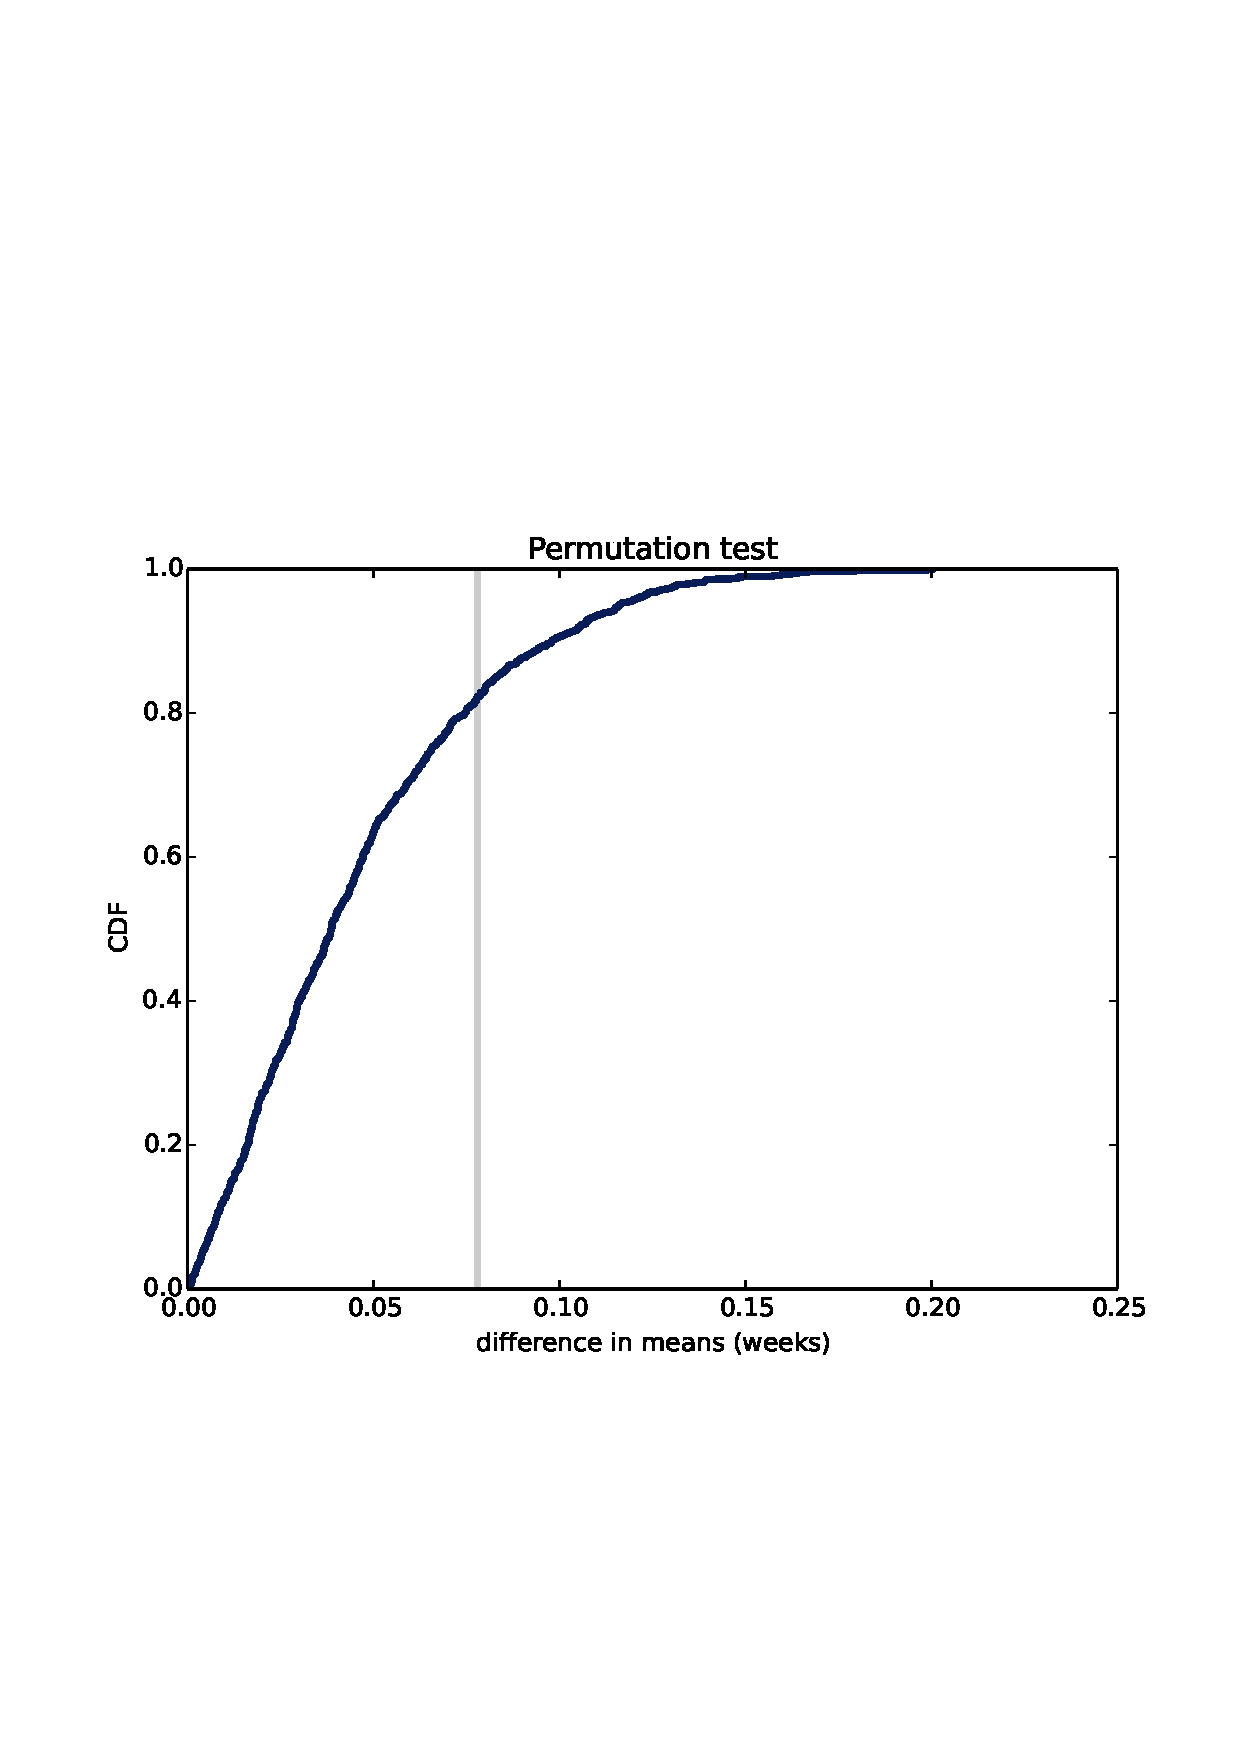
\includegraphics[height=2.5in]{figs/hypothesis1.pdf}}
\caption{귀무가설 아래 평균임신기간 차이 CDF.}
\label{hypothesis1}
\end{figure}

{\tt HypothesisTest}에는 {\tt PlotCdf}가 있는데 관측 효과 크기를 나타내는 회색선과 검정 통계량 분포를 플롯으로 그린다.
\index{thinkplot}
\index{HypothesisTest}
\index{Cdf}
\index{효과 크기 (effect size)}

\begin{verbatim}
    ht.PlotCdf()
    thinkplot.Show(xlabel='test statistic',
                   ylabel='CDF')
\end{verbatim}

그림~\ref{hypothesis1}에 결과가 있다.
CDF는 0.83에서 관측 차이와 교차하는데, p-값의 보수 0.17이다.

 shows the result.  The CDF intersects the
observed difference at 0.83, which is the complement of the p-value,
0.17.
\index{p-값 (p-value)}

만약 출생 체중으로 동일한 분석을 실행한다면, 계산된 p-값은 0 이다; 1000 번 시험 후에, 모의시험은 결코 관측 차이가 0.12 lbs 보다 큰 효과를 산출하지 못한다.
그래서, $p < 0.001$ 가 나오고, 출생 체중에 차이는 통계적으로 유의하다고 결론낸다. 

\index{출생 체중 (birth weight)}
\index{체중 (weight)!출생 (birth)}
\index{유의성 (significant)} 
\index{통계적 유의성 (statistically significant)}


\section{다른 검정 통계량 (ther test statistics)}

최선의 검정 통계량을 고르는 것은 무슨 질문을 하느냐에 달려 있다.
예를 들어, 만약 관련된 질문이 첫번째 아이에 대해서 임신 기간이 다른지에 관한 것이라면, 앞절에서 수행했던 것과 같이, 평균에 대해 차이 절대값을 검정하는 것이 의미가 있다.

\index{검정 통계량 (test statistic)}
\index{임신 기간 (pregnancy length)}

만약 첫번째 아이가 늦게 출생하는 경향이 있다고 생각할 이유가 있다면, 차이값의 절대값을 취하지 않는다; 대신에 다음 검정 통계량을 사용한다.

\begin{verbatim}
class DiffMeansOneSided(DiffMeansPermute):

    def TestStatistic(self, data):
        group1, group2 = data
        test_stat = group1.mean() - group2.mean()
        return test_stat
\end{verbatim}

{\tt DiffMeansOneSided}은 {\tt DiffMeansPermute}에서 {\tt MakeModel}와 {\tt RunModel}을 상속받는다; 유일한 차이는 {\tt TestStatistic}가 
차이에 절대값을 취하지 않는다는 것이다.
이런 유형의 검증을 {\bf 단측 (one-sided)} 검증이라고 한다. 왜냐하면,
차이 분포의 단측면만 고려하기 때문이다. 앞선 검정은 양쪽을 사용하기 때문에 {\bf 양측 (two-sided)} 검증이라고 한다.
\index{단측 검증 (one-sided test)}
\index{양측 검증 (two-sided test)}

이 버젼 검정에 대해서, p-값은 0.09 다. 일반적으로 단측 검정에 대한 p-값은 양측 검정에 대한 p-값의 약 절반이다. 물론 분포 모양에 달려있다.

\index{p-값 (p-value)}

단측 가설, 첫째 아이가 늦게 태어난다는 것이 양측 가설보다 좀더 구체적이다. 그래서 p-값이 더 작다. 하지만, 더 강한 가정에 조차도, 차이는 통계적으로 유의적이지 않다.

\index{유의성 (significant)} 
\index{통계적 유의성 (statistically significant)}

동일한 프레임워크(framework)를 사용해서 표준 편차에 차이도 검정할 수 있다. 
~\ref{visualization} 절에서 첫번째 아이가 늦게 혹은 빨리 출산할 것같은 증거를 일부 보았다. 그래서, 표준 편차가 좀더 클 것이라는 가설을 세울 수 있다. 다음에 이 가설을 시험하는 방법이 있다.

\index{표준 편차 (standard deviation)}

\begin{verbatim}
class DiffStdPermute(DiffMeansPermute):

    def TestStatistic(self, data):
        group1, group2 = data
        test_stat = group1.std() - group2.std()
        return test_stat
\end{verbatim}

이것은 단측 검정인데 이유는 가설이 첫번째 아이 집단에 대한 표준편차가 단지 다르다는 것이 아니라 더 높다는 것이다. p-값이 0.09로, 통계적으로 유의적이지 않다.

\index{p-값 (p-value)}
\index{순열 (permutation)}
\index{유의성 (significant)} 
\index{통계적 유의성 (statistically significant)}


\section{상관 검정 (Testing a correlation)}
\label{corrtest}

상기 프레임워크를 사용해서 상관도 검정할 수 있다. 
예를 들어, NSFG 데이터셋에서, 산모 나이와 출생 체중 사이 상관관계는 약 0.07 이다. 
나이가 많은 산모 아이가 더 체중이 나가는 것처럼 보인다. 하지만 이 효과가 우연에 의한 것일까요?
\index{상관 (correlation)}
\index{검정 통계량 (test statistic)}

검정 통계량으로, 피어슨 상관을 사용했지만, 스피어만 상관도 동일하게 동작한다. 만약 양의 상관 관계로 예측하는 합리적 논거가 있다면, 단측 검정을 할 수도 있다. 하지만, 그런 이유가 없기 때문에, 상관 절대값을 사용해서 양측검정을 수행한다.
\index{피어슨 상관계수 (Pearson coefficient of correlation)}
\index{스피어만 상관계수 (Spearman coefficient of correlation)}

귀무 가설은 산모 연령과 출생 체중 사이에 상관 관계가 없다는 것이다.
관측값을 뒤섞어서, 산모 연령과 출생 체중 분포가 같지만 변수 사이에 관련이 없는 세상을 모의 시험할 수 있다.
\index{출생 체중 (birth weight)}
\index{체중 (weight)!출생 (birth)}
\index{귀무 가설 (null hypothesis)}

\begin{verbatim}
class CorrelationPermute(thinkstats2.HypothesisTest):

    def TestStatistic(self, data):
        xs, ys = data
        test_stat = abs(thinkstats2.Corr(xs, ys))
        return test_stat

    def RunModel(self):
        xs, ys = self.data
        xs = np.random.permutation(xs)
        return xs, ys
\end{verbatim}

{\tt data}는 한쌍 시퀀스다. {\tt TestStatistic}가 피어슨 상관 절대값을 계산한다. {\tt RunModel}이 {\tt xs}를 뒤섞고 모의시험한 데이터를 반환한다.
\index{HypothesisTest}
\index{순열 (permutation)}
\index{피어슨 상관계수 (Pearson coefficient of correlation)}

다음에 데이터를 읽어 들이고, 시험을 수행하는 코드가 있다.

\begin{verbatim}
    live, firsts, others = first.MakeFrames()
    live = live.dropna(subset=['agepreg', 'totalwgt_lb'])
    data = live.agepreg.values, live.totalwgt_lb.values
    ht = CorrelationPermute(data)
    pvalue = ht.PValue()
\end{verbatim}

{\tt subset} 인자로 {\tt dropna}를 사용해서 필요한 변수 둘 중에서 결측된 행을 뺀다.
\index{dropna}
\index{NaN}
\index{결측값 (missing values)}

실제 상관계수는 0.07이다. 계산된 p-값은 0 이다; 1000 번 반복한 뒤에, 가장 큰 모의 시험 상관계수 p-값은 0.04다. 그래서, 관측된 상관계수가 작을지라도, 통계적 유의성이 있다.
\index{p-값 (p-value)}
\index{유의성 (significant)} 
\index{통계적 유의성 (statistically significant)}

``통계적 유의성 (statistically significant)''이 항상 효과가 중요하거나, 실무에서 유의적이라는 의미는 아니라는 것을 상기 예제가 상기 시킨다.
단지 유연으로 발생할 것 같지 않는다는 의미다.

\section{비율 검정 (Testing proportions)}
\label{casino}
\index{카이제곱 검정 chi-squared test}

카지노를 운영한다고 가정합시다. 그런데 고객 한명이 비뚤어진 주사위를 사용하고 있다고 용의선상에 올려놓는다; 즉, 다른 쪽보다 한쪽 면이 더 많이 나오도록 변형한 주사위. 주인장이 주장하는 사기꾼을 체포하고 주사위를 압수했다. 하지만, 이제 주사위가 비뚤어졌다는 것을 주인장이 증명해야 한다.
주사위를 60번 던져서 다음과 같은 결과를 얻었다.
\index{카지노 (casino)}
\index{주사위 (dice)}
\index{비뚤어진 주사위 (crooked die)}

\begin{center}
\begin{tabular}{|l|c|c|c|c|c|c|}
\hline
Value     &  1  &  2  &  3  &  4  &  5  &  6  \\ 
\hline
Frequency &  8  &  9  &  19  &  5  &  8  &  11  \\
\hline
\end{tabular}
\end{center}

평균적으로 주사위 각 값은 10번씩 나올 것으로 예상된다.
데이터셋에서, 값 3이 기대한 것보다 더 자주 나오고, 값 4는 덜 나오는 것 처럼 보인다.하지만, 이 차이가 통계적으로 유의적일까요?
\index{빈도 (frequency)}
\index{유의성 (significant)} 
\index{통계적 유의성 (statistically significant)}

가설을 검정하기 위해서, 각 값에 대한 기대 빈도, 기대 빈도와 관측 빈도 차이, 전체 절대값 차이를 계산할 수 있다. 상기 예제에서, 주사위 각 면은 60 회 중에서 10 회 나올 것으로 예상된다; 이 기대값에서 편차가 -2, -1, 9, -5, -2, 1 이 된다; 그래서 전체 절대값 차이는 20 이 된다. 우연히 이러한 차이를 얼마나 자주 목도할까?
\index{편차 (deviation)}

다음에 상기 질문에 대답하는 {\tt HypothesisTest} 버젼이 있다.
\index{HypothesisTest}

\begin{verbatim}
class DiceTest(thinkstats2.HypothesisTest):

    def TestStatistic(self, data):
        observed = data
        n = sum(observed)
        expected = np.ones(6) * n / 6
        test_stat = sum(abs(observed - expected))
        return test_stat

    def RunModel(self):
        n = sum(self.data)
        values = [1, 2, 3, 4, 5, 6]
        rolls = np.random.choice(values, n, replace=True)
        hist = thinkstats2.Hist(rolls)
        freqs = hist.Freqs(values)
        return freqs
\end{verbatim}

데이터는 빈도 리스트로 표현된다: 관측값은 {\tt [8, 9, 19, 5, 8, 11]}이 되고 ; 기대 빈도는 모두 10 이다.
검정 통계량은 절대값 차이의 총합이다.
\index{빈도 (frequency)}

귀무 가설은 주사위가 공정하다는 것으로 {\tt values} 에서 난수 표본을 뽑아 모의 시험한다. {\tt RunModel} 은 {\tt Hist}를 사용해서 계산하고, 빈도 리스트를 반환한다.

\index{Hist}
\index{귀무 가설 (null hypothesis)}
\index{모형 (model)}

이 데이터에 대한 p-값은 0.13으로 의미하는 바는 만약 주사위가 공정하다면, 전체 관측 편차를 약 13\% 가능성으로 볼 것으로 기대된다. 그래서, 명백한 효과는 통계적으로 유의하지 않다.
\index{p-값 (p-value)}
\index{편차 (deviation)}
\index{유의성 (significant)} 
\index{통계적 유의성 (statistically significant)}


\section{카이제곱 검정 (Chi-squared tests)}
\label{casino2}

이전 절에서 검정 통계량으로 총편차를 사용했다. 하지만,
비율을 검정하는데, 카이제곱 통계량을 사용하는 것이 좀더 일반적이다.
%
\[ \goodchi^2 = \sum_i \frac{(O_i - E_i)^2}{E_i} \]
%
%% TODO: Consider using upper case chi, which is more strictly correct,
%% but harder to distinguish from X.
% 

여기서, $O_i$는 관측빈도, $E_i$는 기대빈도다. 다음에 파이썬 코드가 있다.
\index{카이제곱 검정 (chi-squared test)}
\index{카이제곱 통계량 (chi-squared statistic)}
\index{검정 통계량 (test statistic)}

\begin{verbatim}
class DiceChiTest(DiceTest):

    def TestStatistic(self, data):
        observed = data
        n = sum(observed)
        expected = np.ones(6) * n / 6
        test_stat = sum((observed - expected)**2 / expected)
        return test_stat
\end{verbatim}

(절대값을 취하기 보다)편차를 제곱하면 큰 편차에 더 많은 가중치를 준다.
{\tt expected}로 나누게 되면 편차를 표준화한다. 이 경우에 기대 빈도가 모두 같아서 효과가 없다.

\index{편차 (deviation)}

카이제곱 통계량을 사용한 p-값은 0.04로 총편차를 사용해서 얻은 0.13보다도 훨씬 작다. 만약 5\% 분계점을 심각하게 생각한다면, 효과가 통계적으로 유의하다고 고려할 수 있다. 하지만, 검정 두가지를 모두 고려해서, 결과는 경계선에 있다고 말할 수 있다. 주사위가 삐뚤어졌다는 가능성을 배제하지는 않지만, 고발된 사기꾼에게 유죄 판결을 하지는 않을 것이다.

\index{p-값 (p-value)}
\index{유의성 (significant)} 
\index{통계적 유의성 (statistically significant)}

상기 예제는 중요한 점을 시연해 준다: p-값이 검정 통계량과 귀무 가설 모형에 달려있다. 그리고 때때로, 이러한 선택에 따라 효과가 통계적으로 유의성을 갖거나 갖지 않거나 결정된다.
\index{귀무 가설 (null hypothesis)}
\index{모형 (model)}


\section{다시 첫째 아이}

이장 앞에서 첫번째 아이와 첫째가 아닌 아이들에 대한 임신 기간을 살펴봤고, 평균과 표준편차에 명백한 차이는 통계적으로 유의적이지 않다고 결론냈다. 하지만, ~\ref{visualization} 절에서 평균 기간 분포에서 명백한 차이를 몇가지 봤다. 특히, 35주에서 43주차 범위에서 그렇다. 이러한 차이가 통계적 유의성이 있는지 살펴보기 위해서, 카이제곱 통계량에 기반한 검정을 사용할 수 있다.
\index{표준 편차 (standard deviation)}
\index{통계적 유의성 (statistically significant)} 
\index{유의성 (significant)}
\index{임신 기간 (pregnancy length)}

다음 코드는 앞선 예제로부터 요소를 결합한다.

\index{HypothesisTest}

\begin{verbatim}
class PregLengthTest(thinkstats2.HypothesisTest):

    def MakeModel(self):
        firsts, others = self.data
        self.n = len(firsts)
        self.pool = np.hstack((firsts, others))

        pmf = thinkstats2.Pmf(self.pool)
        self.values = range(35, 44)
        self.expected_probs = np.array(pmf.Probs(self.values))

    def RunModel(self):
        np.random.shuffle(self.pool)
        data = self.pool[:self.n], self.pool[self.n:]
        return data
\end{verbatim}

데이터는 두개 임신 기간 리스트로 표현된다. 귀무가설은
표본 모두 동일한 분포에서 추출되었다는 것이다.
{\tt MakeModel}은 {\tt hstack}을 사용해서 두 표본을 합동(pooling)해서 분포를 모형화한다. 그리고 나서, {\tt RunModel}은 합동 표본을 뒤섞고 이것을 두 부분으로 쪼갬으로써 모의 실험 데이터를 생성한다.
\index{귀무 가설 (null hypothesis)}
\index{모형 (model)}
\index{hstack}
\index{임신 기간 (pregnancy length)}

{\tt MakeModel}은 또한 {\tt values}를 정의하는데, 사용할 주차 범위가 되고, 
\verb"expected_probs"는 합동 분포(pooled distribution)에서 각 값의 확률이다.

다음에 검정 통계량을 계산하는 코드가 있다.

\begin{verbatim}
# class PregLengthTest:

    def TestStatistic(self, data):
        firsts, others = data
        stat = self.ChiSquared(firsts) + self.ChiSquared(others)
        return stat

    def ChiSquared(self, lengths):
        hist = thinkstats2.Hist(lengths)
        observed = np.array(hist.Freqs(self.values))
        expected = self.expected_probs * len(lengths)
        stat = sum((observed - expected)**2 / expected)
        return stat
\end{verbatim}

{\tt TestStatistic}은 첫째 아이와 첫째 아이가 아닌 아이들에 대한 카이제곱 통계량을 계산하고 더한다.
\index{카이제곱 통계량 (chi-squared statistic)}

{\tt ChiSquared}는 임신 기간 시퀀을 받아, 히스토그램을 계산하고,
{\tt observed}를 계산하는데, 이는 {\tt self.values}에 상응하는 빈도 리스트다. 기대 빈도 리스트를 계산하기 위해서, 표본 크기에 미리 계산된 확률 \verb"expected_probs"을 곱한다. 그러면 카이제곱 통계량 {\tt stat}을 반환한다.

NSFG 데이터에 대해서, 전체 카이제곱 통계량은 102로 그 자체로 많은 것을 의미하지는 않는다. 하지만, 1000회 반복 후에, 귀무가설 아래에서 가장 큰 검정 통계량은 32다. 관측 카이제곱 통계량이 귀무가설 아래에서 가능할 것 같지 않다고 결론내린다. 그래서, 외관 효과는 통계적 유의성이 있다.

\index{귀무 가설 (null hypothesis)}
\index{통계적 유의성 (statistically significant)} 
\index{유의성 (significant)}

이번 예제는 카이제곱 검정 한계를 보여준다: 두 집단 사이에 차이가 있다는 것을 나타내지만, 차이가 무엇인지에 관한 구체적인 어떤 것도 말하지는 못한다.

\section{오류 (Errors)}
\index{오류 (error)}

전통적인 가설 검정에서 만약 p-값이 특정 분계점, 흔히 5\% 보다 아래라면, 통계적 유이성이 있다고 본다. 이러한 절차는 두가지 질문을 불러온다.
\index{p-값 (p-value)}
\index{분계점 (threshold)}
\index{통계적 유의성 (statistically significant)} 
\index{유의성 (significant)}

\begin{itemize}

\item 만약 효과가 실제로 우연으로 인한다면, 효과를 잘못해서 유의적으로 고려할 확률은 얼마나 될까? 이 확률이 {\bf 거짓 양성률 (false positive rate)}이다.
\index{거짓 양성 (false positive)}

\item 만약 효과가 진실이라면, 가설 검정이 실패할 가능성은 얼마나 될까?
이 확률이 {\bf 거짓 음성률 (false negative rate)}이다.
\index{거짓 음성 (false negative)}

\end{itemize}

거짓 양성률은 상대적으로 계산하기 쉽다: 만약 분계점이 5\% 이면, 거짓 양성률은 5\% 다. 다음에 이유가 있다.

\begin{itemize}

\item 만약 실제 효과가 없다면, 귀무 가설은 사실이다. 그래서 귀무 가설을 모의 시험함으로써, 검정 통계량 분포를 계산할 수 있다. 이 분포를 $\CDF_T$ 라고 부른다.
\index{귀무 가설 (null hypothesis)}
\index{CDF}

\item 실험을 매번 실행할 때마다, 검정 통계량 $t$ 를 얻는데, $CDF_T$에서 뽑아낸 것이다. 그리고 나서, p-값을 계산하는데, $CDF_T$에서 나온 난수 값이 {\tt t}를 초과하는 확률이다. 그래서 $1 - CDF_T(t)$이 된다.

\item 만약 $CDF_T(t)$가 95\%보다 크다면, p-값이 5\% 보다 작다; 즉, 만약 $t$가 95번째 백분위수를 초과하면 그렇다. 그리고, $CDF_T$에서 고른 값이 95번째 백분위수를 얼마나 자주 초과할까? 거의 5\% 다.

\end{itemize}

그래서, 5\% 분계점을 가진 가설 검정을 수행한다면, 거짓 양성이 20번 중 1번 예상된다. 

\section{검정력 (Power)}
\label{power}

거짓 음성률은 계산하기 더 어렵다. 왜냐하면, 실제 효과 크기에 의존하고 정상적으로는 실제 효과 크기를 모르기 때문이다. 한가지 선택옵션은 가상 효과크기(hypothetical effect size) 조건으로 거짓 음성률을 계산하는 것이다.
\index{효과 크기 (effect size)}

예를 들어, 만약 두 집단 사이에 관측 차이가 정확하다면, 관측 표본을 모집단 모형으로 사용해서 모의 시험 데이터로 가설 검정을 실행할 수 있다.
\index{모형 (model)}

\begin{verbatim}
def FalseNegRate(data, num_runs=100):
    group1, group2 = data
    count = 0

    for i in range(num_runs):
        sample1 = thinkstats2.Resample(group1)
        sample2 = thinkstats2.Resample(group2)

        ht = DiffMeansPermute((sample1, sample2))
        pvalue = ht.PValue(iters=101)
        if pvalue > 0.05:
            count += 1

    return count / num_runs
\end{verbatim}

{\tt FalseNegRate}는 각 집단마다 하나씩 두 시퀀스 형태로 데이터를 받는다.

루프를 매번 돌 때마다, 각 집단에서 난수 표본을 뽑아서 가설 검정을 실행함으로써 실험을 모의 시험한다. 그리고 나서 결과를 확인하고 거짓 음성 갯수를 계수한다.
\index{Resample}
\index{순열 (permutation)}

{\tt Resample}은 시퀀스를 받아 복원 추출로 동일 길이를 가진 표본을 뽑는다.
\index{복원 (replacement)}

\begin{verbatim}
def Resample(xs):
    return np.random.choice(xs, len(xs), replace=True)
\end{verbatim}

다음에 임신 기간을 검정하는 코드가 있다.

\begin{verbatim}
    live, firsts, others = first.MakeFrames()
    data = firsts.prglngth.values, others.prglngth.values
    neg_rate = FalseNegRate(data)
\end{verbatim}

결과가 약 70\%로 의미하는 바는 만약 평균 임신기간에 실제 차이가 0.078 주라면, 이 표본 크기를 가진 실험은 대략 70\% 음성 검정을 산출할 것으로 기대된다.
\index{임신 기간 (pregnancy length)}

이 결과는 종종 다르게 제시된다: 만약 실제 차이가 0.078 주라면, 
대략 30\% 만 양성 검정을 기대해야 한다. 
이 ``정확한 양성률 (correct positive rate)''이 검정 {\bf 검정력(power)}이라고 부르고, 종종 ``민감도 (sensitivity)''라고 한다. 주어진 크기 효과를 탐지하는 검정 능력을 반영한다.
\index{검정력 (power)}
\index{민감도 (sensitivity)}
\index{정확한 양성 (correct positive)}

이 예제에서, 검정은 단지 30\% 가능성만으로 양성 결과를 산출한다(다시, 차이가 0.078 주라는 것을 가정하면). 경험 법칙으로, 80\% 검정력이 납득할 수 있는 수준이다. 그래서 이 검정은 ``검정력 부족 (underpowered)''하다고 말할 수 있다.
\index{검정력 부족 (underpowered)}

일반적으로 음성 가설 검정이 두 집단 사이에 차이가 없다는 것을 의미하는 것은 아니다; 대신에 만약 차이가 있다면, 너무 작아서 표본크기로 탐지할 수 없다는 것을 제시한다.

\section{반복 (Replication)}
\label{replication}

이번 장에서 시연한 가설검정과정은 엄밀히 말하면 좋은 관례(good practice)는 아니다.

첫째, 다중 검정(multiple tests)을 수행했다. 만약 가설 검정 하나를 실행한다면, 거짓양성(false positive) 가능성은 약 20번 중에 한번으로 수용가능하다. 하지만, 20번 검정을 수행한다면, 대부분 적어도 한번은 거짓양성을 예상해야한다.
\index{다중 검정 (multiple tests)}

둘째, 탐색과 검정에 동일한 데이터셋을 사용했다. 만약 대용량 데이터셋을 탐색하고, 놀라운 효과를 발견하고 나서, 효과가 유의성이 있는지 검정한다면, 거짓 양성(false positive)을 생성할 가능성이 있다.

\index{통계적 유의성 (statistically significant)} 
\index{유의성 (significant)}

다중 검정을 보상하기 위해서, p-값 분계점을 조정할 수 있다. (\url{https://en.wikipedia.org/wiki/Holm-Bonferroni_method} 참조). 혹은, 한 데이터셋은 탐색, 다른 데이터셋은 검정으로 데이터를 분할해서 두 문제를 다룰 수 있다. 
\index{p-값 (p-value)}
\index{홈-본페로니 법 (Holm-Bonferroni method)}

몇몇 분야에서는 이러한 관례가 요구되고 있거나 적어도 장려한다. 하지만, 이러한 문제를 암묵적으로 출판된 결과를 반복(replication)하면서 다루는 것도 흔하다. 전형적으로, 새로운 결과를 보고하는 첫번째 논문은 탐색적으로 고려된다. 새로운 데이터로 결과를 반복하는 이어지는 논문은 확증적(confirmatory)으로 고려된다.
\index{확증적 결과 (confirmatory result)}

공교롭게도, 이 장에서 결과를 반복할 기회가 있다.
이책 첫번째 판은 2002년에 나온 NSFG 사이클 6에 기반했다.
2011년 10월 CDC가 2006--2010에 실시한 인터뷰에 기반한 추가 데이터를 출시했다. {\tt nsfg2.py} 에는 이 데이터를 읽고 정제한 코드가 포함되어 있다. 새로운 데이터셋으로 분석한 결과는 다음과 같다.
\index{NSFG}

\begin{itemize}

\item 평균 임신 기간에 차이는 0.16 주다. $p < 0.001$ 으로 통계적 유의성이 있다. (원본 데이터셋 0.078주와 비교된다.)

\index{통계적 유의성 (statistically significant)} 
\index{유의성 (significant)}
\index{임신 기간 (pregnancy length)}

\item 출생 체중에 차이는 0.17 파운드로 $p < 0.001$ 이다.
(원본 데이터셋 0.12 lbs와 비교된다.)
\index{출생 체중 (birth weight)}
\index{체중 (weight)!출생 (birth)}

\item 출생 체중과 산모 연령 사이 상관계수는 0.08 로 $p < 0.001$ 이다. (0.07과 비교된다.).

\item 카이제곱검정은 $p < 0.001$ 으로 통계적 유의성이 있다.
$p < 0.001$ (원본 데이터도 그렇다.).

\end{itemize}

요약하면, 원본 데이터에서 통계적 유의성이 있는 모든 효과가 새로운 데이터셋에서도 반복되었다. 그리고 임신기간에 차이는 원데이터에서 유의성이 없었으나 새로운 데이터셋에서는 더 커졌고 유의성이 있다.


\section{연습 문제}

이 연습문제에 대한 해답은 \verb"chap09soln.py" 파일에 나와있다.

\begin{exercise}
표본크기가 증가함에 따라, 가설검정력은 증가하는데,
효과가 실제하면 좀더 양성임을 의미한다.
반대로, 표본크기가 줄어들면, 검정력은 설사 효과가 실제한다고 하더라도 덜 양성일 것 같다.
\index{표본크기}

이런 작동방식을 조사하는데, NSFG 데이터에서 다른 일부 데이터를 갖는 검정을 실시한다.
{\tt thinkstats2.SampleRows}을 사용해서, 데이터프레임에 임의로 행일부를 선택한다.

\index{가족성장 국가조사}
\index{NSFG}
\index{데이터프레임}

표본크기가 감소함에 따라 검정 p-값에는 무슨 일이 일어나는가?
양의 검정을 산출하는 최소 표본크기는 얼마인가?

\index{p-값}
\end{exercise}


\begin{exercise}

\ref{testdiff}~절에서, 
순열로 귀무가설을 모의시험했다; 즉,
관측된 값을 마치 전체 모집단을 대표하는 것처럼 다루었고,
무작위로 모집단의 구성원을 두 집단에 배정했다.
\index{귀무가설}
\index{순열}

대안은 표본을 사용해서 모집단 분포를 추정하고 나서, 분포로부터 임의 표본을 추출하는 것이다.
이런 과정을 {\bf 재표집(resampling)}이라고 부른다.
재표집을 구현하는 몇가지 방식이 있지만, 가장 단순한 것중 하나가 \ref{power}~처럼 관측된 값에서 복원방식으로 표본을 추출하는 것이다.

\index{재표집}
\index{복원}

{\tt DiffMeansPermute}에서 상속받고, 순열보다 재표집을 구현하는 {\tt RunModel}을 
치환(override)하는 클래스 {\tt DiffMeansResample}을 작성하시오.
\index{순열}

이 모형을 사용해서 임신기간과 출생체중 사이 차이를 검정하시오.
이 모형이 결과에 얼마나 영향을 주는가?
\index{모형}
\index{출생체중}
\index{체중!출생}
\index{임신기간}

\end{exercise}


\section{용어 사전}

\begin{itemize}

\item 가설 검정 (hypothesis testing): 외관 효과(apparent effect)가 통계적 유의성이 있는지 결정하는 과정.
\index{가설 검정 (hypothesis testing)}

\item 검정 통계량 (test statistic): 효과 크기를 정량화하는데 사용되는 통계량.
\index{검정 통계량 (test statistic)}
\index{효과 크기 (effect size)}

\item 귀무 가설 (null hypothesis): 외관 효과가 우연에 의한 것이라는 가정에 기반한 시스템 모델.
\index{귀무 가설 (null hypothesis)}

\item p-값 (p-value): 효과가 우연에 의해서 발생한 확률.
\index{p-값 (p-value)}

\item 통계적 유의성 (statistically significant): 우연에 의해서 발생할 것 같지 않다면, 효과는 통계적 유의성이 있다.
\index{통계적 유의성 (statistically significant)} 
\index{유의성 (significant)}

\item 순열 검정 (permutation test): 관측 데이터셋에서 순열을 생성해서 p-값을 계산하는 방법.
\index{순열 검정 (permutation test)}

\item 재표본 검정 (resampling test): 관측 데이터셋에서 복원으로 표본을 생성해서 p-값을 계산하는 방법.
\index{재표본 검정 (resampling test)}

\item 양측 검정 (two-sided test): ``효과 크기가 양으로 혹은 음으로 관측 효과보다 얼마나 큰가?'' 를 묻는 검정.

\item 단측 검정 (one-sided test): ``효과 크기가 동일 부호로 관측 효과보다 얼마나 큰가?'' 를 묻는 검정.
\index{단측 검정 (one-sided test)}
\index{양측 검정 (two-sided test)}
\index{검정 (test)!단측 (one-sided)}
\index{검정 (test)!양측 (two-sided)}

\item 카이-제곱 검정 (chi-squared test): 검정 통계량으로 카이-제곱 통계량을 사용하는 검정.
\index{카이-제곱 검정 (chi-squared test)}

\item 거짓 양성 (false positive): 사실이 아닐 때, 효과가 사실이라는 결론.
\index{거짓 양성 (false positive)}

\item 거짓 음성 (false negative): 우연이 아닐 때 효과가 우연 때문이라는 결론.
\index{거짓 음성 (false negative)}

\item 검정력 (power): 대립가설이 사실일 때, 이를 사실로서 결정할 확률이다. 검정력이 90\%라고 하면, 대립가설이 사실임에도 불구하고 귀무가설을 채택할 확률은 10\%이다.\footnote{\url{http://ko.wikipedia.org/wiki/검정력} 참조}
\index{검정력 (power)}
\index{귀무 가설 (null hypothesis)}

\end{itemize}





\chapter{선형최소제곱 (Linear least squares)}
\label{linear}

이번 장에서 사용되는 코드는 {\tt linear.py}에 있다.
코드를 다운로드하고 작업하는 것에 대한 정보는 ~\ref{code}을 참조한다.

\section{최소제곱 적합 (Least squares fit)}

상관계수는 관계 부호와 강도를 측정하지만 기울기는 측정하지 않는다.
기울기를 측정하는 방법이 몇가지 있다; 가장 흔한 방법이 {\bf 선형최소제곱 적합 (linear least squares fit)}이다. ``선형 적합(linear fit)''은 변수 사이 관계를 모형화하는 선(line)이다.
``최소제곱 (least squares)'' 적합은 선과 데이터 사이 평균제곱오차(mean
squared error, MSE)를 최소화하는 것이다.
\index{최소제곱 적합 (least squares fit)}
\index{선형최소제곱 (linear least squares)}
\index{모형 (model)}

하나 시퀀스 {\tt ys}가 있는데, 또 다른 시퀀스 {\tt xs} 함수로 표현하고자 한다고 가정하자.
만약 {\tt xs}, {\tt ys}와 절편 {\tt inter}, 기울기 {\tt slope} 사이에 선형 관계가 있다면,
각 {\tt y[i]} 가 {\tt inter + slope * x[i]}이 될 것으로 예상된다.  
\index{잔차 (residuals)}

하지만, 상관이 완벽하지 않다면, 예측은 단지 근사(approximation)가 된다.
선에서 수직 편차(vertical deviation), 즉 {\bf 잔차(residual)}는 다음과 같다. 
\index{편차 (deviation)}

\begin{verbatim}
res = ys - (inter + slope * xs)
\end{verbatim}

잔차는 측정 오차 같은 확률 요소(random factor), 혹은 알지 못하는 비임의 요소(non-random factor) 때문일지 모른다. 예를 들어, 만약 체중을 신장 함수로 예측한다면, 미지 요소는 식습관, 운동, 신체 유형을 포함할 수 있다.

\index{기울기 (slope)}
\index{절편 (intercept)}
\index{측정 오차 (measurement error)}

만약 모수 {\tt inter}와 {\tt slope}이 잘못되면, 잔차는 더 커진다.
그래서 모수는 잔차를 최소화한다는 것이 직관적으로 의미가 있다.
\index{모수 (parameter)}

잔차 절대값, 잔차 제곱, 혹은 잔차 세제곱 최소화를 시도해볼만 하다;
하지만, 가장 흔한 선택은 제곱 잔차 합을 최소화하는 것이다. {\tt sum(res**2))}.

왜 그럴까요? 세가지 좋은 이유와 한가지 덜 중요한 이유가 있다.

\begin{itemize}

\item 제곱하게 되면 양수 잔차와 음수 잔차를 동일하게 처리하는 기능이 있는데, 보통 원하는 것이다.

\item 제곱은 큰 잔차에 더 많은 가중치를 주지만, 가장 큰 잔차가 항상 주도적인 경우에는 그렇게 많은 가중치를 주지는 않는다.

\item 만약 잔차가 상관관계가 없고 평균과 상수 (하지만 알려지지 않은 미지) 분산을 가진 정규분포라면,
최소제곱 적합은 또한 {\tt inter}와 {\tt slope}의 최대우도추정량이다. \url{https://en.wikipedia.org/wiki/Linear_regression}.  
\index{MLE}
  \index{최대우도추정량 (maximum likelihood estimator)}
\index{상관 (correlation)}

\item 제곱 잔차를 최소화하는 {\tt inter}와 {\tt slope} 값은 효과적으로 계산될 수 있다.

\end{itemize}

계산 효율성(computational efficiency)이 당면한 문제에 가장 적합한 방법을 선택하는 것보다 더 중요할 때 마지막 이유가 의미있다. 
이제는 더 이상 그럴지는 않다. 그래서, 제곱 잔차가 최소화하는 올바른 것인지만 고려한다.
\index{계산 방법 (computational methods)}
\index{제곱잔차 (squared residuals)}

예를 들어, {\tt xs}을 사용해서 {\tt ys} 값을 예측하려고 한다면,
과다 추정하는 것이 과소 추정하는 것보다 더 좋을 수도 (더 나쁠 수도) 있다.
이런 경우, 각 잔차에 대한 비용함수를 계산하고 전체 비용, {\tt sum(cost(res))}을 최소화한다.
하지만, 최소제곱 적합을 계산하는 것이 빠르고, 쉽고, 종종 충분히 만족스럽다.
\index{비용 함수 (cost function)}


\section{구현 (Implementation)}

{\tt thinkstats2}에 선형최소제곱을 시연하는 간단한 함수가 있다.
\index{LeastSquares}

\begin{verbatim}
def LeastSquares(xs, ys):
    meanx, varx = MeanVar(xs)
    meany = Mean(ys)

    slope = Cov(xs, ys, meanx, meany) / varx
    inter = meany - slope * meanx

    return inter, slope
\end{verbatim}

{\tt LeastSquares}는 시퀀스 {\tt xs}와 {\tt ys}을 인자로 받고 추정한 모수 {\tt inter}와
{\tt slope}을 반환한다. 동작방법에 관한 자세한 사항은 웹사이트 참조. \url{http://wikipedia.org/wiki/Numerical_methods_for_linear_least_squares}.
\index{모수 (parameter)}


{\tt thinkstats2}는 {\tt FitLine}를 제공하는데, {\tt inter} 와 {\tt slope}을 인자로 받아서 시퀀스 {\tt xs}에 대해서 적합선을 반환한다.
\index{FitLine}

\begin{verbatim}
def FitLine(xs, inter, slope):
    fit_xs = np.sort(xs)
    fit_ys = inter + slope * fit_xs
    return fit_xs, fit_ys
\end{verbatim}

이 함수를 사용해서 산모 연령 함수로 출생 체중에 대한 최소제곱을 계산할 수 있다.
\index{출생 체중 (birth weight)}
\index{체중 (weight)!출생 (birth)}
\index{연령 (age)}

\begin{verbatim}
    live, firsts, others = first.MakeFrames()
    live = live.dropna(subset=['agepreg', 'totalwgt_lb'])
    ages = live.agepreg
    weights = live.totalwgt_lb

    inter, slope = thinkstats2.LeastSquares(ages, weights)
    fit_xs, fit_ys = thinkstats2.FitLine(ages, inter, slope)
\end{verbatim}

추정한 절편과 기울기는 년마다 6.8 lbs, 0.017 lbs 이다.
이러 형태로 값을 해석하기는 어렵다: 절편은 산모 연령이 0 에서 신생아 기대 체중인데,
문맥상 의미가 없고, 기울기는 너무 작아서 쉽게 이해가 되지 않는다.
\index{기울기 (slope)}
\index{절편 (intercept)}
\index{dropna}
\index{NaN}


$x=0$에 절편을 제시하는 대신에, 절편을 평균에 제시하는 것이 종종 도움이 된다.
이 경우에, 평균 나이는 약 25세이고, 25세 산모에 대한 평균 아이 체중은 7.3 파운드다.
기울기는 년마다 0.27 온스(ounces) 즉, 10년마다 0.17 파운드가 된다.

\begin{figure}
% linear.py
\centerline{\includegraphics[height=2.5in]{figs/linear1.pdf}}
\caption{선형적합한 산모연령과 출생체중 산점도.}
\label{linear1}
\end{figure}

그림~\ref{linear1}에 적합선과 함께 출생 체중과 연령을 산점도로 보여준다.
이와 같이, 관계가 선형인지, 적합선이 관계를 나타내는 좋은 모형인지를 평가하는데, 그림을 그려보는 것은 좋은 생각이 된다. 

\index{출생 체중 (birth weight)}
\index{체중 (weight)!출생 (birth)}
\index{산점도 (scatter plot)}
\index{그림 (plot)!산점 (scatter)}
\index{모형 (model)}


\section{잔차 (Residuals)}
\label{residuals}

또다른 유용한 검정은 잔차를 플롯하여 그리는 것이다.
{\tt thinkstats2}에는 잔차를 계산하는 함수가 있다.
\index{잔차 (residuals)}

\begin{verbatim}
def Residuals(xs, ys, inter, slope):
    xs = np.asarray(xs)
    ys = np.asarray(ys)
    res = ys - (inter + slope * xs)
    return res
\end{verbatim}

{\tt Residuals}는 시퀀스 {\tt xs}와 {\tt ys}, 추정한 {\tt inter}와 {\tt slope}를 인자로 받는다. 실제값과 적합선 사이 차이를 반환한다.

\begin{figure}
% linear.py
\centerline{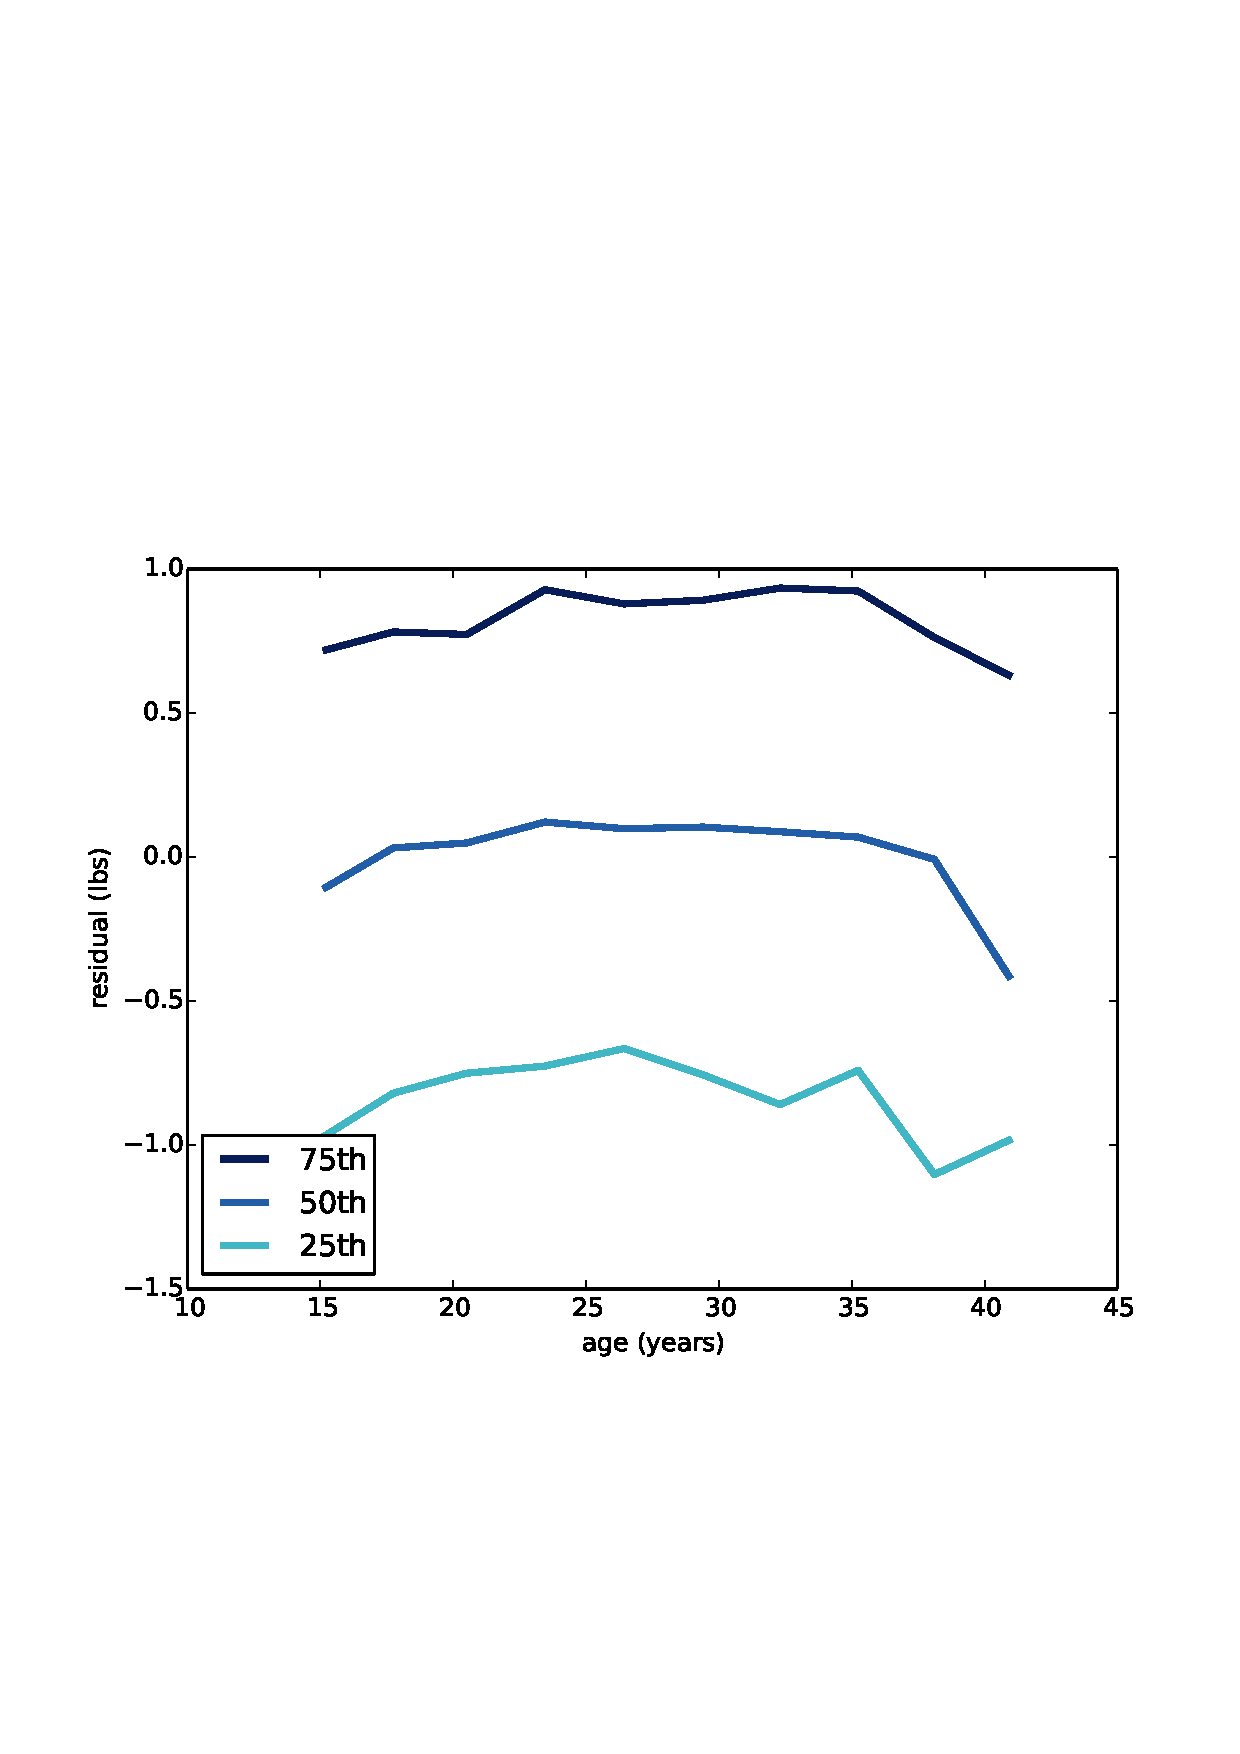
\includegraphics[height=2.5in]{figs/linear2.pdf}}
\caption{선형적합 잔차.}
\label{linear2}
\end{figure}

잔차를 시각화하기 위해서, ~\ref{characterizing} 절에서 살펴본 것과 같이, 응답자를 연령으로 묶고, 각 집단에 백분위수를 계산한다. 
그림~\ref{linear2}에 각 연령 집단에 대한 25번째, 50번째, 75번째 백분위수가 있다.
중위수는 예상한 것처럼 거의 0이고, 사분위수 범위는 약 2 파운드다. 그래서, 만약 산모 연령을 알고 있다면, 1 파운드 내에서 대략 50\% 가능성으로 아이 체중을 추측할 수 있다.
\index{시각화 (visualization)}

이상적으로 이들 직선이 평평해서 잔차가 랜덤(random)임을 나타내고, 
평행해서 잔차 분산이 모든 연령 집단에 대해서 동일하다는 것을 나타내야 한다.
사실, 직선은 평행에 가깝워서 좋다; 하지만, 약간의 곡률(curvature)이 있어서 관계가 비선형임을 나타낸다.
그럼에도 불구하고, 선형 적합은 간단한 모형으로 특정 목적에 아마도 잘 부합한다.  

\index{모형 (model)}
\index{비선형 (nonlinear)}


\section{추정 (Estimation)}
\label{regest}

모수 {\tt slope}와 {\tt inter}는 표본에 기반한 추정값이다; 다른 추정값처럼, 표집 편의, 측정 오차, 표집 오차에 휘둘리기 쉽다. 
~\ref{estimation} 장에서 논의한 것처럼, 표집 편의는 비대표 표집(non-representative sampling)에 의해서, 측정 오차는 데이터 수집과 기록 오류에 의해서, 표집 오차는 전체 모집단보다 표본을 측정하는 결과로 발생한다.
\index{표집 편의 (sampling bias)}
\index{편의 (bias)!표집 (sampling)}
\index{측정 오차 (measurement error)}
\index{표집 오차 (sampling error)}
\index{추정 (estimation)}

표집 오차를 평가하기 위해서, ``만약 이 실험을 다시 실행한다면,
추정값에 얼마나 변동성이 예상될까?''
이러한 질문에 모의시험 실험을 진행하고, 추정값에 대한 표집 분포를 계산함으로써 대답할 수 있다.

\index{표집 오차 (sampling error)}
\index{표집 분포 (sampling distribution)}

데이터를 재표본추출(resampling)하으로써 실험을 모의시험할 수 있다; 즉, 관측된 임신을 마치 전체 모집단인 것처럼 처리해서 관측된 표본에서 복원 추출 방식으로 표본을 추출한다.
\index{모의 시험 (simulation)}
\index{복원 (replacement)}

\begin{verbatim}
def SamplingDistributions(live, iters=101):
    t = []
    for _ in range(iters):
        sample = thinkstats2.ResampleRows(live)
        ages = sample.agepreg
        weights = sample.totalwgt_lb
        estimates = thinkstats2.LeastSquares(ages, weights)
        t.append(estimates)

    inters, slopes = zip(*t)
    return inters, slopes
\end{verbatim}

{\tt SamplingDistributions} 함수는 인자로 정상 출산마다 한 줄(row)로 된 데이터프레임과 모의 시험 실험 횟수, {\tt iters}를 인자로 받는다. {\tt ResampleRows}을 사용해서 관측 임신을 재표본추출한다. 이미 {\tt SampleRows}를 살펴봤는데, 데이터프레임에서 무작위(random) 행을 선택한다. {\tt thinkstats2}는 또한 {\tt ResampleRows} 기능도 제공하는데, 원본과 동일한 크기 표본을 반환한다.
\index{데이터프레임 (DataFrame)}
\index{재표본추출 (resampling)}

\begin{verbatim}
def ResampleRows(df):
    return SampleRows(df, len(df), replace=True)
\end{verbatim}

재표본추출 후에, 모의 시험 표본을 사용해서 모수를 추정한다.
결과는 시퀀스 두개다: 추정 절편과, 추정 기울기.

\index{모수 (parameter)}

표준 오차와 신뢰구간을 출력해서 표집 분포를 요약한다.
\index{표집 분포 (sampling distribution)}

\begin{verbatim}
def Summarize(estimates, actual=None):
    mean = thinkstats2.Mean(estimates)
    stderr = thinkstats2.Std(estimates, mu=actual)
    cdf = thinkstats2.Cdf(estimates)
    ci = cdf.ConfidenceInterval(90)
    print('mean, SE, CI', mean, stderr, ci)
\end{verbatim}

{\tt Summarize}는 추정값과 실제값 시퀀을 인자로 받는다. 추정값 평균, 표준 오차, 그리고, 90\% 신뢰구간을 출력한다.
\index{표준 오차 (standard error)}
\index{신뢰 구간 (confidence interval)}

절편에 대해서, 평균 추정값은 6.83, 표준오차(SE)는 0.07, 90\% 신뢰구간(CI) (6.71, 6.94)이다. 좀더 간략한 형식으로, 추정 절편 0.0174, SE 0.0028, CI (0.0126, 0.0220)가 된다. 이 신뢰구간 하한과 상한 사이에 거의 두배 차이난다. 그래서, 개략적인 추정값으로 봐야한다.

%inter 6.83039697331 6.83174035366
%SE, CI 0.0699814482068 (6.7146843084406846, 6.9447797068631871)
%slope 0.0174538514718 0.0173840926936
%SE, CI 0.00276116142884 (0.012635074392201724, 0.021975282350381781)

추정값의 표집 오차를 시각화하기 위해서, 적합선을 모두 플롯으로 그리고, 연하게 채워서 각 연령에 대해서 90\% 신뢰구간을 플롯으로 그린다. 다음에 코드가 있다.

\begin{verbatim}
def PlotConfidenceIntervals(xs, inters, slopes,
                            percent=90, **options):
    fys_seq = []
    for inter, slope in zip(inters, slopes):
        fxs, fys = thinkstats2.FitLine(xs, inter, slope)
        fys_seq.append(fys)

    p = (100 - percent) / 2
    percents = p, 100 - p
    low, high = thinkstats2.PercentileRows(fys_seq, percents)
    thinkplot.FillBetween(fxs, low, high, **options)
\end{verbatim}

{\tt xs}는 산모 연령 시퀀스다. {\tt inters}와 {\tt slopes}는 {\tt SamplingDistributions}에서 생성된 추정 모수다. {\tt percent} 인자는 플롯을 얼마의 신뢰구간으로 그릴 것인지 나타낸다.

{\tt PlotConfidenceIntervals}는 {\tt inter}와 {\tt slope} 짝에 대해 적합선을 생성하고, 결과를 시퀀스 \verb"fys_seq"에 저장한다.
그리고 나서, {\tt PercentileRows}을 사용해서 {\tt x} 각 값에 대해서 {\tt y} 상한과 하한 백분위수를 선택한다. 
90\% 신뢰구간에 대해서, 5번째와 95번째 백분위수를 선택한다. 
{\tt FillBetween}은 두 직선 사이 공간을 채우는 다각형을 그린다.
\index{thinkplot}
\index{FillBetween}

\begin{figure}
% linear.py
\centerline{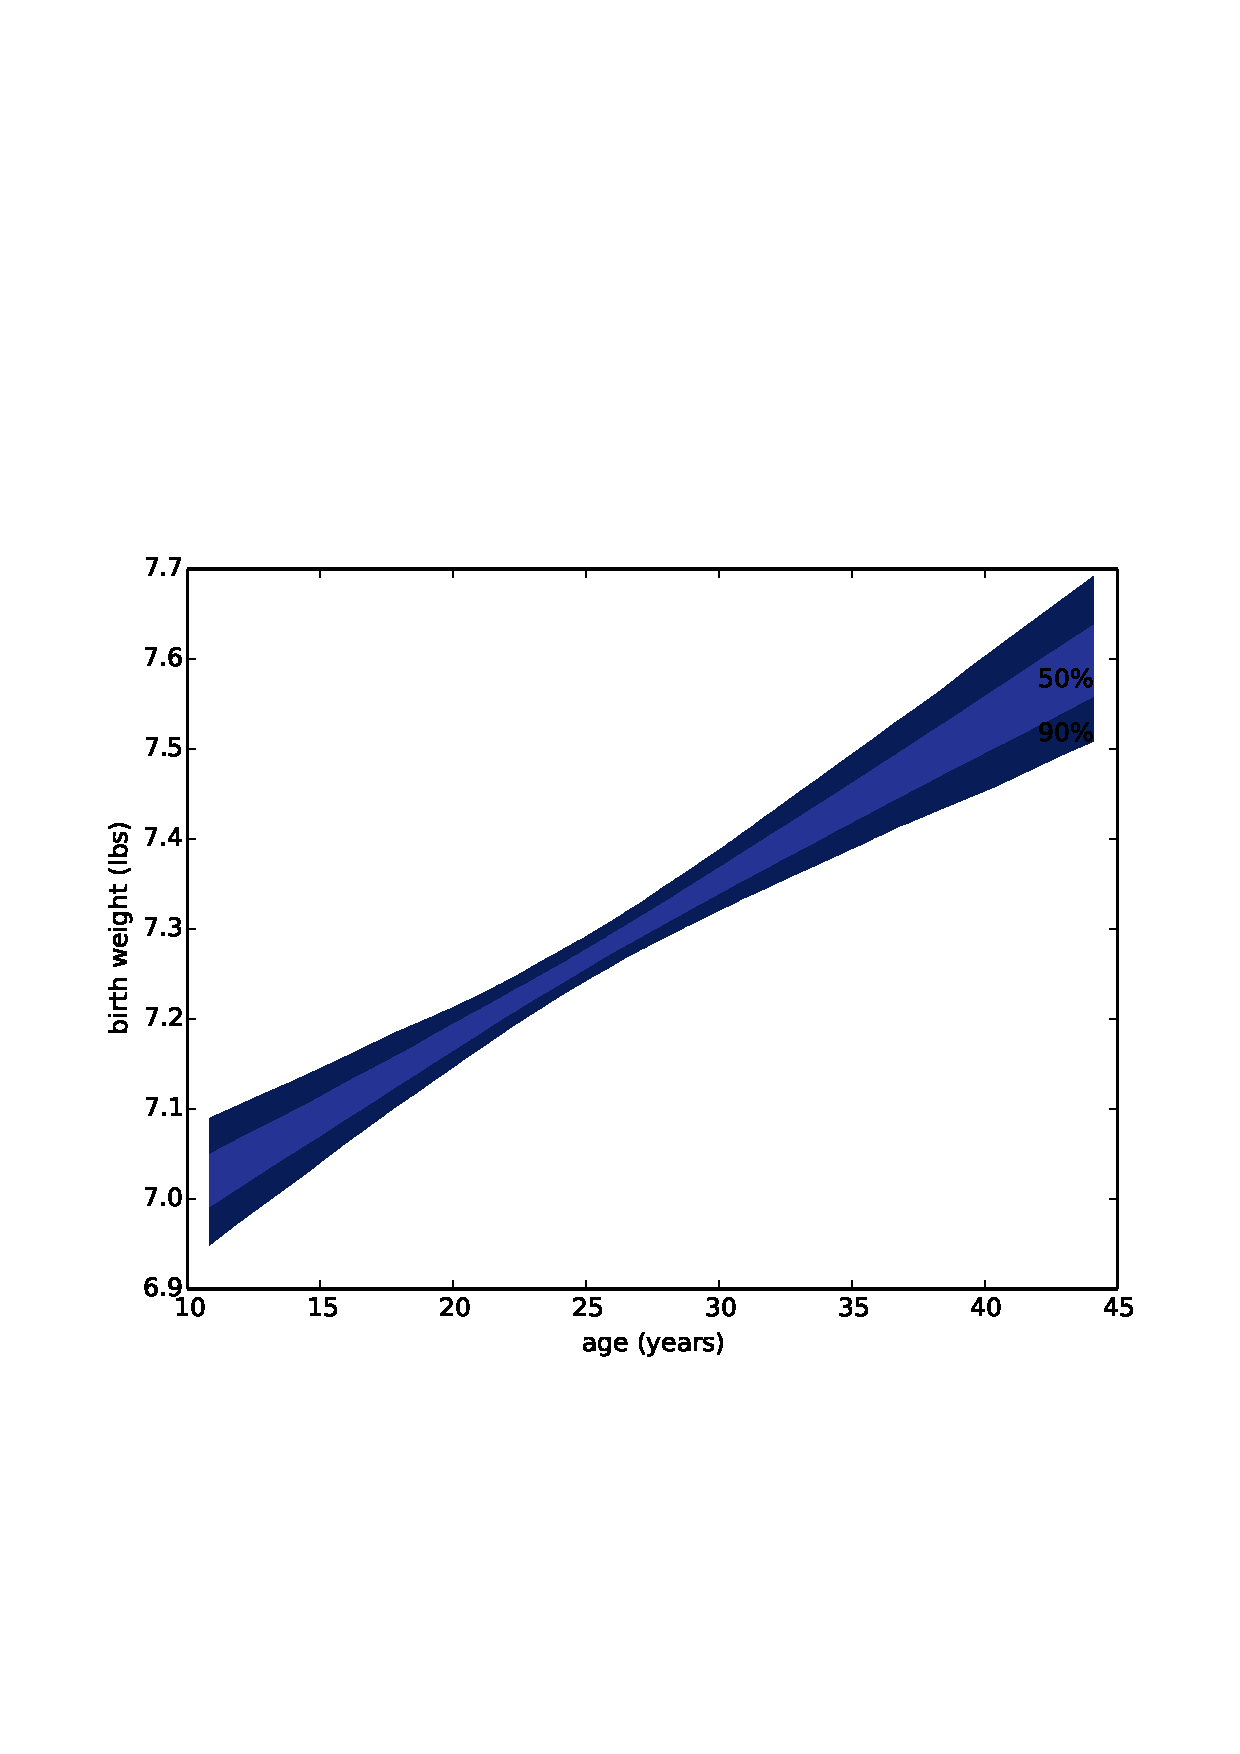
\includegraphics[height=2.5in]{figs/linear3.pdf}}
\caption{{\tt inter} 와 {\tt slope} 표집오차 때문에,
적합선에 변동성을 나타내는 신뢰구간 50\% 와 90\%.}
\label{linear3}
\end{figure}

그림~\ref{linear3}에는 산모 연령에 대한 함수로 출생 체중에 적합된 곡선에 대한 50\% 와 90\% 신뢰구간이 있다. 구역의 수직폭(vertical width)이 표집 오차에 대한 효과를 표현한다; 효과가 평균 주변 값에 대해 더 작고, 극단값에 대해 더 크다.

\section{적합도 (Goodness of fit)}
\label{goodness}
\index{적합도 (goodness of fit)}

선형 모형 품질, 즉 {\bf 적합도 (goodness of fit)}를 측정하는 방법이 몇가지 있다. 가장 간단한 방법은 잔차의 표준편차다.

\index{표준 편차 (standard deviation)}
\index{모형 (model)}

만약 예측을 위해 선형 모형을 사용한다면, {\tt Std(res)}는 예측의 제곱근 평균제곱오차(root mean squared error, RMSE)다.
예를 들어, 만약 출생 체중을 추측하는데 산모 연령을 사용한다면, 추측 RMSE는 1.40 lbs가 된다.
\index{출생 체중 (birth weight)}
\index{체중 (weight)!출생 (birth)}

만약 산모 나이를 모른 상태에서 출생 체중을 추측한다면, 
추측 RMSE는 {\tt Std(ys)}로, 1.41 lbs다.  
그래서, 이 예제에서 산모 연령을 알고 있는 것은 그다지 예측력을 향상시키지 못한다.
\index{예측 (prediction)}

적합도를 측정하는 또 다른 방식은 $R^2$로 표기하고, ``R-제곱(R-squared)''라고 부르는 {\bf 결정계수 (coefficient of determination)}다.

\index{결정계수 (coefficient of determination)}
\index{r-제곱 (r-squared)}

\begin{verbatim}
def CoefDetermination(ys, res):
    return 1 - Var(res) / Var(ys)
\end{verbatim}

{\tt Var(res)}는 모형을 사용한 추측 MSE 이고, {\tt Var(ys)}는 
모형없는 MSE 다. 그래서, 비율이 만약 모형을 사용한다면 남게되는 MSE 부분이다. $R^2$ 는 모형이 제거하는 MSE 부분이 된다.
\index{MSE}

출산 체중과 산모 나이에 대해, $R^2$ 값은 0.0047 으로, 산모 나이가 출생 체중에 있는 분산 약 0.5\%만 예측한다는 의미가 된다.

결정계수와 피어슨 상관계수 사이에 간단한 관계가 있다: $R^2 = \rho^2$.
예를 들어, 만약 $\rho$ 가 0.8 혹은 -0.8 이라면, $R^2 = 0.64$가 된다.
\index{피어슨 상관계수 (Pearson coefficient of correlation)}

$\rho$와 $R^2$가 종종 관계 강도를 정량화하는데 사용될지라도,
예측력(predictive power)에 대해서 해석하기는 쉽지 않다.
저자 견해로는, {\tt Std(res)}가 예측 품질을 가장 잘 표현한다고 본다. 특히, 만약 {\tt Std(ys)}와 연관되어 표현되면 그렇다. 

\index{결정계수 (coefficient of determination)}
\index{r-제곱 (r-squared)}

예를 들어, SAT(미국 대학 입학시험에 사용되는 표준국가시험) 타당성에 대해서 얘기할 때, 종종 사람들은 SAT 점수와 다른 지능(IQ) 측정값 사이에 상관을 얘기한다.
\index{SAT}
\index{지능 (IQ)}

한 연구에 의하면, SAT 점수와 IQ 점수 사이에 피어슨 상관은 $\rho=0.72$ 으로, 강한 상관처럼 보인다.
하지만, $R^2 = \rho^2 = 0.52$ 이여서 SAT 점수는 IQ 분산의 단지 52\%만 설명한다.

IQ 점수는 {\tt Std(ys) = 15} 로 정규화된다. 그래서, 

\begin{verbatim}
>>> var_ys = 15**2
>>> rho = 0.72
>>> r2 = rho**2
>>> var_res = (1 - r2) * var_ys
>>> std_res = math.sqrt(var_res)
10.4096
\end{verbatim}

IQ 예측하는데 SAT 점수를 사용하는 것은 RMSE를 15 점에서 10.4 점으로 줄인다. 상관계수 0.72 는 RMSE 를 줄이는데 단지 31\% 기여한다.

만약 상관계수가 감명적으로 보인다면, $R^2$이 MSE 축소에 더 나은 지표가 되고, RMSE 축소가 예측력에 대한 더 나은 지표다.

\index{결정계수 (coefficient of determination)}
\index{r-제곱 (r-squared)}
\index{예측 (prediction)}


\section{선형 모형 검정 (Testing a linear model)}

출생 체중에 대한 산모 연령 효과가 작고, 거의 예측력이 없다.
그래서, 외관 관계(apparent relationship)가 유연에 의해서 가능한 것인가?
선형적합 결과를 검정하는 방법이 몇개 있다.
\index{출생 체중 (birth weight)}
\index{체중 (weight0!출생 (birth)}
\index{모형 (model)}
\index{선형 모형 (linear model)}

한 선택옵션은 MSE에 외관 축소(apparent reduction)가 우연에 의한 것인지 검정하는 것이다. 이 경우에 검정 통계량은 $R^2$ 이고, 귀무 가설은 변수 간 관계가 없다가 된다. ~\ref{corrtest} 절에서 산모 연령과 출생 체중 간 상관을 검정했을 처럼, 귀무가설을 순열(permutation)을 통해서 모의 시험할 수 있다. 사실, $R^2 = \rho^2$, 이기 때문에, $R^2$ 단측 검정은 $\rho$ 양측 검정과 상응한다. 이미 이 검정을 수행했고, $p < 0.001$ 라는 것을 발견했다. 그래서, 산모 연령과 출생 체중 간 외관 관계는 통계적 유의성이 있다고 결론낸다.

\index{귀무 가설 (null hypothesis)}
\index{순열 (permutation)}
\index{결정계수 (coefficient of determination)}
\index{r-제곱 (r-squared)}
\index{유의성 (significant)} 
\index{통계적 유의성 (statistically significant)}

또 다른 접근법은 외관 기울기(apparent slope)가 우연에 의한 것인지 검정하는 것이다. 귀무가설은 기울기가 실제로 0 이다는 것이다; 이 경우에, 출생 체중을 평균 근처에 확률변동(random variation)으로 모형화할 수 있다. 다음에 이 모형에 대한 HypothesisTest 가 있다.
\index{HypothesisTest}
\index{모형 (model)}

\begin{verbatim}
class SlopeTest(thinkstats2.HypothesisTest):

    def TestStatistic(self, data):
        ages, weights = data
        _, slope = thinkstats2.LeastSquares(ages, weights)
        return slope

    def MakeModel(self):
        _, weights = self.data
        self.ybar = weights.mean()
        self.res = weights - self.ybar

    def RunModel(self):
        ages, _ = self.data
        weights = self.ybar + np.random.permutation(self.res)
        return ages, weights
\end{verbatim}

데이터는 연령과 체중 시퀀스로 표현된다.
검정 통계량은 {\tt LeastSquares}로 추정된 기울기다.
귀무 가설 모형은 모든 아기들의 평균 체중과 평균에 대한 편차로 표현된다.
모의 시험 데이터를 생성하기 위해서, 편차를 순열로 배치하고, 평균에 더한다.

\index{편차 (deviation)}
\index{귀무가설 (null hypothesis)}
\index{순열 (permutation)}

다음에 가설 검정을 수행하는 코드가 있다.

\begin{verbatim}
    live, firsts, others = first.MakeFrames()
    live = live.dropna(subset=['agepreg', 'totalwgt_lb'])
    ht = SlopeTest((live.agepreg, live.totalwgt_lb))
    pvalue = ht.PValue()
\end{verbatim}

p-값이 $0.001$ 보다 작다, 그래서 설사 추정된 기울기가 작지만, 우연에 의한 것 같지는 않다.

\index{p-값 (p-value)}
\index{dropna}
\index{NaN}

귀무가설을 모의 시험함으로써 p-값을 추정하는 것이 엄격하게는 맞다. 하지만, 더 간단한 대안이 있다. 이미 ~\ref{regest} 절에서 기울기 표집 분포를 계산한 것을 기억하라. 이를 위해서, 관측된 기울기가 맞다고 가정하고 재표본추출(resampling)으로 실험을 모의 시험했다.

\index{귀무가설 (null hypothesis)}

그림~\ref{linear4}에는 ~\ref{regest}절과 귀무가설 아래에서 생성된 기울기 분포에서 나온 기울기 표집 분포가 있다.
표집 분포가 추정된 기울기 약 0.017 lbs/년을 중심으로 있고, 귀무가설 아래 기울기가 약 0 을 중심으로 있다; 하지만, 그것을 제외하고 분포는 동일한다. 분포는 또한 ~\ref{CLT}절에서 살펴보게될 이유로 대칭이다. 
 
\index{대칭 (symmetric)}
\index{표집 분포 (sampling distribution)}

\begin{figure}
% linear.py
\centerline{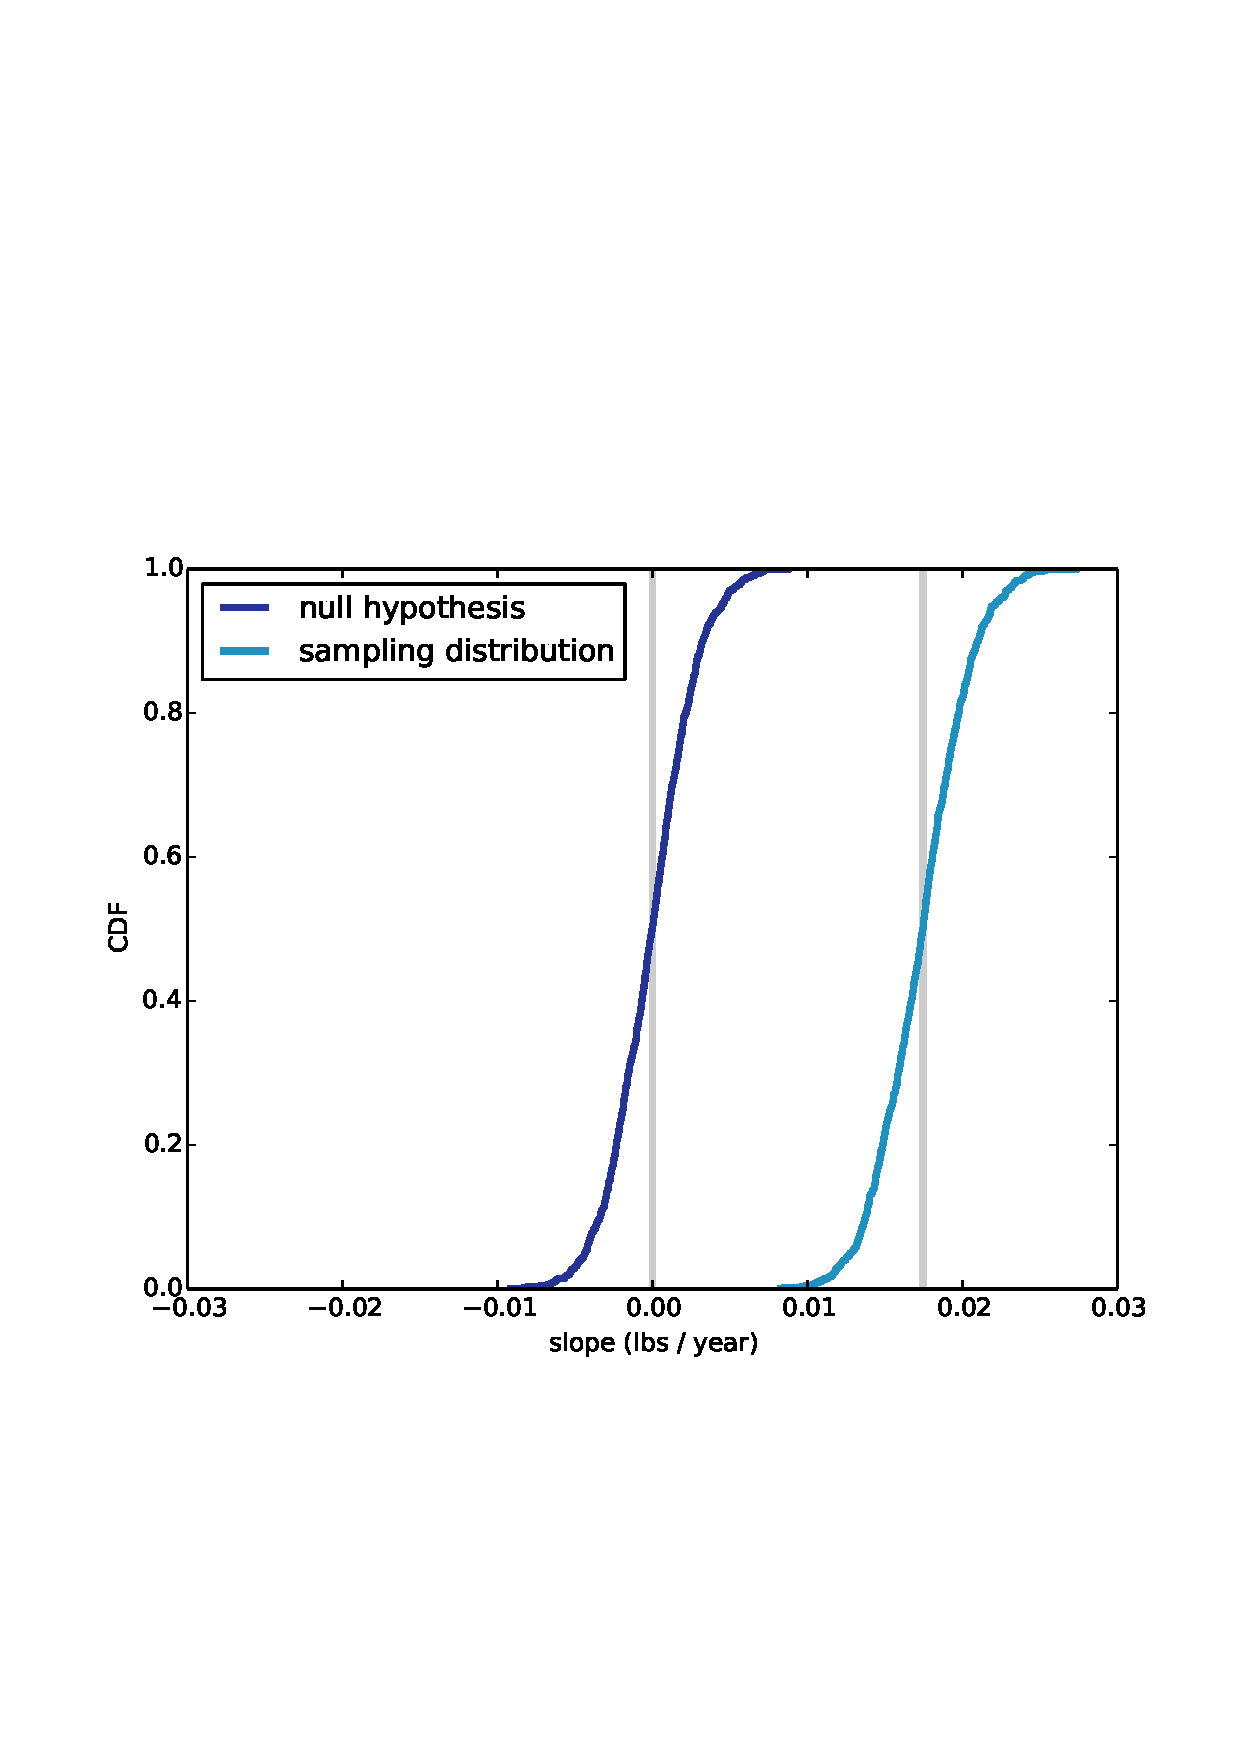
\includegraphics[height=2.5in]{figs/linear4.pdf}}
\caption{귀무가설아래 생성된 기울기 분포와 추정 기울기에 대한 표집 분포. 수직선은 0과 관측 기울기는 0.017 파운드/년.}
\label{linear4}
\end{figure}

그래서, p-값을 두 방식으로 추정할 수 있다:
\index{p-값 (p-value)}

\begin{itemize}

\item 귀무가설 아래서 기울기가 관측 기울기를 초과할 확률을 계산한다.
\index{귀무가설 (null hypothesis)}

\item 표집분포에서 기울기가 0 이하인 확률을 계산한다. (만약 추정 기울기가 음수라면, 표집 분포에서 기울기가 0을 초과하는 확률을 계산할 것이다.)

\end{itemize}

두번째 선택옵션은 더 쉬운데 이유는 어떻든 정상적으로 모수의 표집 분포를 계산하고자 하기 때문이다. 그리고 표본 크기가 작지 않고, {\em 그리고} 잔차 분포가 기울지 않았다면 좋은 근사(approximation)가 된다. 그때조차도, p-값이 정교할 필요가 없기 때문에, 대체로 만족스럽다.

\index{왜도 (skewness)}
\index{모수 (parameter)}

다음에 표집분포를 사용해서 기울기 p-값을 추정하는 코드가 있다.
\index{표집 분포 (sampling distribution)}

\begin{verbatim}
    inters, slopes = SamplingDistributions(live, iters=1001)
    slope_cdf = thinkstats2.Cdf(slopes)
    pvalue = slope_cdf[0]
\end{verbatim}

다시한번, $p < 0.001$이 나온다.  


\section{가중 재표본추출 (Weighted resampling)}
\label{weighted}

지금까지 NSFG 데이터를 마치 대표 표본인 것처럼 다루었다. 하지만, ~\ref{nsfg} 절에서 언급한 것 같이, 대표 표본은 아니다. 의도적으로 조사는 몇몇 집단을 오버샘플링(oversampling) 하는데 이유는 통계적으로 유의적인 결과를 도출할 확률을 높이기 위해서다; 즉, 이들 집단에 대해서 검정력을 향상하기 위해서다.
\index{유의성 (significant)} 
\index{통계적 유의성 (statistically significant)}

조사설계가 많은 목적에 대해서 유용하지만, 표집 과정을 고려하지 않고, 일반 모집단에 대한 값을 추정하는데 표본을 사용할 수 있다는 것을 의미하지는 않는다.

각 응답자에 대해서, NSFG 데이터는 {\tt finalwgt} 변수가 있는데, 응답자가 대표하는 일반 모집단에 속한 사람 숫자다. 이 값은 {\bf 표집 가중치 (sampling weight}, 즉 ``가중치 (weight)''라고 불린다.
\index{표집 가중치 (sampling weight)}
\index{가중치 (weight)}
\index{가중 재표본추출 (weighted resampling)}
\index{재표본추출 (resampling)!가중 (weighted)}

예제로, 만약 3억 인구를 가진 나라에서 100,000 명을 조사한다면, 각 응답자는 3,000 명을 대표한다. 만약 한 집단을 2배 오버샘플링한다면, 오버샘플링된 집단에 각 사람은 더 적은 가중치(약 1500)가 된다.

오버샘플링을 보정하기 위해서, 재표본추출(resampling)을 사용할 수 있다; 즉, 표집 가중치에 비례하는 확률을 사용해서 조사자료에서 표본을 추출한다.
그리고 나서, 추정하려고 하는 임의 정량정보에 대해서 표집 분포, 표본 오차, 신뢰구간을 생성할 수 있다. 예제로, 평균 출생 체중을 표본 가중치를 두고, 안두고 추정할 것이다.

\index{표본 오차 (standard error)}
\index{신뢰 구간 (confidence interval)}
\index{출생 체중 (birth weight)}
\index{체중 (weight)!출생 (birth)}
\index{표집 분포 (sampling distribution)}
\index{오버샘플링 (oversampling)}

~\ref{regest}절에서, {\tt ResampleRows}를 살펴봤다. 동일한 확률을 각 행에 두고 데이터프레임에서 행을 추출한다. 이제 동일한 것을 표집 가중치에 비례한 확률을 사용해서 수행할 필요가 있다. {\tt ResampleRowsWeighted}는 데이터프레임을 인자로 받고, {\tt finalwgt}에 있는 가중치에 따라 행을 재표본 추출하고, 재표본추출된 행을 포함하는 데이터프레임을 반환한다.

\index{데이터프레임 (DataFrame)}
\index{재표본추출 (resampling)}

\begin{verbatim}
def ResampleRowsWeighted(df, column='finalwgt'):
    weights = df[column]
    cdf = Cdf(dict(weights))
    indices = cdf.Sample(len(weights))
    sample = df.loc[indices]
    return sample
\end{verbatim}

{\tt weights}는 시리즈다; 시리즈를 딕셔너리로 전환하는 것은 인덱스를 가중치로 매핑한다. {\tt cdf}에서 값은 인덱스고, 확률은 가중치에 비례한다.

{\tt indices}는 행인덱스 시퀀스다; {\tt sample}은 선택된 행을 담고 있는 데이터프레임이다. 복원 표본 추출을 했기 때문에, 동일한 행이 한번이상 나올 수 있다.
\index{Cdf}
\index{복원 (replacement)}

이제, 가중치를 두고, 두지 않고 재표본추출 효과를 비교할 수 있다.
가중치를 두지 않고, 다음과 같이 표집분포를 생성한다.
\index{표집 분포 (sampling distribution)}

\begin{verbatim}
    estimates = [ResampleRows(live).totalwgt_lb.mean()
                 for _ in range(iters)]
\end{verbatim}

가중치를 두면, 다음과 같다.

\begin{verbatim}
    estimates = [ResampleRowsWeighted(live).totalwgt_lb.mean()
                 for _ in range(iters)]
\end{verbatim}

다음 표에 요약결과가 나와있다.

\begin{center}
\begin{tabular}{|l|c|c|c|}
\hline
                    &  mean birth   & standard  &  90\% CI  \\ 
                    &  weight (lbs) & error     &           \\ 
\hline
Unweighted          &  7.27  &  0.014  &  (7.24, 7.29)  \\ 
Weighted            &  7.35  &  0.014  &  (7.32, 7.37)  \\ 
\hline
\end{tabular}
\end{center}

%mean 7.26580789518
%stderr 0.0141683527792
%ci (7.2428565501217079, 7.2890814917127074)
%mean 7.34778034718
%stderr 0.0142738972319
%ci (7.3232804012858885, 7.3704916897506925)

예제애서, 가중치를 둔 효과는 적지만 무시할만하지는 않다.
가중치를 두고, 두지 않고 추정된 평균에 차이는 약 0.08 파운드, 1.3 온스다.
차이가 추정값 표준 오차(0.014 파운드)보다 실질적으로 더 크다. 함축하는 바는 차이는 우연적 요소에 의한 것은 아니라는 것이다.
\index{표준 오차 (standard error)}
\index{신뢰 구간 (confidence interval)}


\section{연습문제}

이 연습문제에 대한 해답은 \verb"chap10soln.ipynb" 파일에 나와있다.

\begin{exercise}

BRFSS에서 나온 데이터를 사용해서, log(체중) 대비 신장에 대한 선형 최소자승적합을 계산하라.
변수중 하나가 로그 변환된 이와 같은 모형에 대해서 
추정된 모수를 나타내는 가장 좋은 방식은 어떻게 될까요?
만약 누군가의 체중을 추측하려고 한다면, 신장을 아는 것이 얼마나 도움이 될까?

\index{행동위험요소 감시시스템}
\index{BRFSS}
\index{모형}

NSFG와 마찬가지로, BRFSS는 일부 집단을 과다표집(oversampling)하고 각 응답자에 대해서 표집 가중치 정보를 제공한다. BRFSS 데이터에서, 해당 가중치에 대한 변수명은 {\tt totalwt}다.
가중치를 갖는, 갖지 않는 재표집을 사용해서, BRFSS에 나온 평균 응답자 신장, 평균에 대한 표준오차, 90\% 신뢰구간을 추정하시오. 보정 가중치가 추정값에 얼마나 영향을 주는가?
\index{신뢰구간}
\index{표준오차}
\index{과다표집}
\index{표집 가중치}
\end{exercise}


\section{용어 사전}

\begin{itemize}

\item 선형적합 (linear fit): 변수 사이 관계를 모형화하려는 직선.
\index{선형적합 (linear fit)}

\item 최소제곱적합 (least squares fit): 잔차제곱합을 최소화하는 데이터셋 모형.
\index{최소제곱적합 (least squares fit)}

\item 잔차 (residual): 실제값과 모형값 편차.
\index{잔차 (residuals)}

\item 적합도 (goodness of fit): 모형이 데이터에 얼마나 잘 적합하는지에 대한 척도.
\index{적합도 (goodness of fit)}

\item 결정계수 (coefficient of determination): 적합도를 계량화하려는 통계량.
\index{결정계수 (coefficient of determination)}

\item 표집 가중치 (sampling weight): 
표본이 모집단 어느 부분을 대표하는지 나타내는데 표본 관측과 연관된 값.
\index{표집 가중치 (sampling weight)}

\end{itemize}




\chapter{회귀 (Regression)}
\label{regression}

앞장에서 선형최소적합은 {\bf 회귀 (regression)}의 한 사례다. 회귀는 어떤 종류의 데이터를 어떤 종류의 모형에도 적합하는 더 일반적인 문제다. ``회귀 (regression)'' 용어 사용은 역사적 우연이다; 단어의 본래 의미와는 간접적으로 연관된다.
\index{모형 (model)}
\index{회귀 (regression)}

회귀분석의 목적은 {\bf 종속변수 (dependent variables)}라고 불리는 변수집합과 {\bf 설명변수 (explanatory variables)}라고 불리는 또 다른 집합변수 사이 관계를 기술하는 것이다.
\index{설명변수 (explanatory variable)}
\index{종속변수 (dependent variable)}

앞장에서 종속변수로 출생 체중을 예측하는데 설명변수로 산모 연령을 사용했다.
단지 종속변수가 하나 설명변수도 하나라면, {\bf 단순회귀(simple regression)}가 된다. 이번 장에서는 하나 이상 설명변수를 갖는 {\bf 다중회귀(multiple regression)}로 옮겨간다. 만약 종속변수가 하나이상이라면, 다변량회귀(multivariate regression)이 된다.
\index{출생 체중 (birth weight)}
\index{체중 (weight)!출생 (birth)}
\index{단순회귀 (simple regression)}
\index{다중회귀 (multiple regression)}


만약 종속변수와 설명변수 간 관계가 선형이면, {\bf 선형회귀 (linear regression)}가 된다. 예를 들어, 종속변수가 $y$이고, 설명변수가 $x_1$과 $x_2$라면, 
다음과 같이 선형회귀모형을 작성할 수 있다.
%
\[ y = \beta_0 + \beta_1 x_1 + \beta_2 x_2 + \eps \]
%

여기서 $\beta_0$는 절편, $\beta_1$은 $x_1$과 연관된 모수, $\beta_2$는 
$x_2$와 연관된 모수, 그리고 $\eps$는 확률변동 혹은 다른 미지 요인으로 인한 잔차다.
\index{회귀모형 (regression model)}
\index{선형회귀 (linear regression)}

$y$에 대한 시퀀스 값과 $x_1$과 $x_2$에 대한 시퀀스 값이 주어지면, $\eps^2$ 합을 최소화하는 $\beta_0$, $\beta_1$, $\beta_2$ 모수를 찾을 수 있다. 이 과정을 {\bf 보통최소제곱(ordinary least squares)}이라고 부른다. 
연산은 {\tt thinkstats2.LeastSquare}와 유사하지만, 하나 이상의 설명변수를 다루도록 일반화되었다. 자세한 정보는 웹사이트를 참조한다. \url{https://en.wikipedia.org/wiki/Ordinary_least_squares}
\index{설명변수 (explanatory variable)}
\index{보통최소제곱 (ordinary least squares)}
\index{모수 (parameter)}

이번 장에서 사용되는 코드는 {\tt regression.py}에 있다.
코드를 다운로드하고 작업하는 것에 대한 정보는 ~\ref{code}을 참조한다.

\section{StatsModels}
\label{statsmodels}

앞장에서 가독성이 좋은 단순선형회귀모형을 구현한 {\tt thinkstats2.LeastSquares}를 제시했다. 다중회귀에 대해서 StatsModels로 전환한다. 파이썬 팩키지로 몇가지 형태 회귀분석와 다른 분석 기능을 제공한다. 만약 아나콘다(Anaconda)를 사용하고 있다면, 이미 StatsModels이 설치되어 있다; 그렇지 않다면, 설치해야할지 모른다.
\index{아나콘다 (Anaconda)}

예제로, StatModels을 가지고 앞장 모형을 실행한다.
\index{StatsModels}
\index{모형 (model)}

\begin{verbatim}
    import statsmodels.formula.api as smf

    live, firsts, others = first.MakeFrames()
    formula = 'totalwgt_lb ~ agepreg'
    model = smf.ols(formula, data=live)
    results = model.fit()
\end{verbatim}

{\tt statsmodels}은 인터페이스(APIs) 두개를 제공한다; ``formula'' API는 문자열로 종속변화 설명변수를 식별한다.
{\tt patsy}라는 구문(syntax)을 사용한다; 상기 예제에서, \verb"~" 연산자가 왼편에 종속변수와 오른편에 설명변수를 구별한다.
\index{설명변수 (explanatory variable)}
\index{종속변수 (dependent variable)}
\index{Patsy}

{\tt smf.ols}는 인자로 문자열 공식과 데이터프레임 {\tt live}를 받고,
모형을 표현하는 OLS객체를 반환한다.
{\tt ols} 는 ``ordinary least squares'' 약자다.
\index{데이터프레임 (DataFrame)}
\index{모형 (model)}
\index{보통최소제곱 (ordinary least squares)}

{\tt fit}메쏘드는 모형을 데이터에 적합하고 결과를 담고 있는 객체 RegressionResults를 반환한다.
\index{RegressionResults}

결과는 또한 속성(attribute)으로도 접근가능하다.
{\tt params}은 시리즈로 변수명을 모수에 매핑한다.
그래서, 다음과 같은 절편과 기울기를 얻을 수 있다.
\index{시리즈 (Series)}

\begin{verbatim}
    inter = results.params['Intercept']
    slope = results.params['agepreg']
\end{verbatim}

추정한 모수는 6.83 와 0.0175으로 {\tt LeastSquares}로 추정한 것과 동일한다.
\index{모수 (parameter)}

{\tt pvalues}는 시리즈로 변수명과 연관된 p-값을 매핑한다.
그래서 추정한 기울기가 통계적으로 유의한지 점검할 수 있다.
\index{p-값 (p-value)}
\index{유의성 (significant)} 
\index{통계적 유의성 (statistically significant)}

\begin{verbatim}
    slope_pvalue = results.pvalues['agepreg']
\end{verbatim}

{\tt agepreg}와 연관된 p-값은 {\tt 5.7e-11} 으로 예상한 것처럼 $0.001$ 보다 적다.
\index{연령 (age)}

{\tt results.rsquared}는 $R^2$ 정보를 담고 있는데 $0.0047$이다.  
{\tt results}는 또한 전체 모형과 연관된 p-값인 \verb"f_pvalue"도 제공하는데 $R^2$가 통계적으로 유의한가를 점검하는 검정과 유사하다. 
\index{모형 (model)}
\index{결정계수 (coefficient of determination)}
\index{r-제곱 (r-squared)}

{\tt results}는 잔차 시퀀스인 {\tt resid}와 {\tt agepreg}에 상응하는 적합한 값 시퀀스 {\tt fittedvalues}도 제공한다.
\index{잔차 (residuals)}

{\tt results} 객체는 {\tt summary()} 메쏘드도 제공하는데,
가독성이 좋은 형식으로 결과를 표현한다.

\begin{verbatim}
    print(results.summary())
\end{verbatim}
하지만 (아직) 관련되지도 않은 많은 정보를 출력한다.
그래서 {\tt SummarizeResults}로 불리는 더 간단한 함수를 사용한다.
다음에 모형 결과가 있다.

\begin{verbatim}
Intercept       6.83    (0)
agepreg         0.0175  (5.72e-11)
R^2 0.004738
Std(ys) 1.408
Std(res) 1.405
\end{verbatim}

{\tt Std(ys)}는 만약 어떤 설명변수 도움없이 출생 체중을 추측해야 한다면 갖게될 종속변수 표준편차 RMSE가 된다.
{\tt Std(res)}는 만약 추측에 산모 연령 정보를 안다면 갖게될 잔차 표준편차 RMSE가 된다. 
이미 살펴봤듯이, 산모 연령을 아는 것이 그다지 예측에 향상을 가져오지는 않는다.

\index{표준편차 (standard deviation)}
\index{출생체중 (birth weight)}
\index{체중 (weight)!출생 (birth)}
\index{설명변수 (explanatory variable)}
\index{종속변수 (dependent variable)}
\index{RMSE}
\index{예측력 (predictive power)}


\section{다중회귀 (Multiple regression)}
\label{multiple}

~\ref{birth_weights}절에서 첫째 아이 체중이 첫째가 아닌 아이들 체중보다 가벼운 경향이 있고, 그 효과가 통계적 유의적성이 있다는 것을 봤다.
하지만, 이상한 결과로 이유는 첫번째 아이 체중이 더 가볍다고 할 수 있는 분명한 메커니즘(mechanism)은 없다. 그래서 이러한 관계가 {\bf 거짓(spurious)}인지 궁금하다.
\index{다중회귀 (multiple regression)}
\index{거짓관계(spurious relationship)}

사실 이 효과에 대한 가능한 설명이 있기는 하다. 출생 체중이 산모 연령에 의존한 것을 봤다. 그리고 첫째 아이 산모는 첫째가 아닌 아이 산모보다 더 어리다는 것을 예상할 수 있다.
\index{체중 (weight)}
\index{연령 (age)}
계산 몇번으로 상기 설명이 그럴듯한지 점검할 수 있다.
그리고 나서, 다중회귀를 사용해서 좀더 자세히 조사할 것이다. 먼저 체중 차이가 얼마나 큰지 살펴본다.

\begin{verbatim}
diff_weight = firsts.totalwgt_lb.mean() - others.totalwgt_lb.mean()
\end{verbatim}

첫째 아이는 0.125 lbs, 즉 2 온스 가볍다. 그리고 연령 차이는 다음과 같다.

\begin{verbatim}
diff_age = firsts.agepreg.mean() - others.agepreg.mean()
\end{verbatim}

첫째 아이 산모 나이가 3.59 년 더 젊다.
다시 선형 모형을 돌리게 되면, 연령 함수로 출생체중에 변화값를 얻는다.
\index{출생 체중 (birth weight)}
\index{체중 (weight)!출생 (birth)}

\begin{verbatim}
results = smf.ols('totalwgt_lb ~ agepreg', data=live).fit()
slope = results.params['agepreg']
\end{verbatim}

기울기는 년당 0.175 파운드다. 만약 기울기를 연령 차이와 곱하게 되면, 산모 연령 때문에 첫째 아이와 첫째가 아닌 아이들에 대한 출생 체중 평균 차이를 얻게된다. 

\begin{verbatim}
slope * diff_age
\end{verbatim}

결과는 0.063 으로 관측 차이의 약 절반이다. 
그래서 잠정적으로 출생 체중에 관측 차이는 부분적으로 산모 연령 차이로 설명될 수 있다고 결론낸다.

다중 회귀를 사용해서, 관계를 좀더 체계적으로 탐색할 수 있다.
\index{다중 회귀 (multiple regression)}

\begin{verbatim}
    live['isfirst'] = live.birthord == 1
    formula = 'totalwgt_lb ~ isfirst'
    results = smf.ols(formula, data=live).fit()
\end{verbatim}

첫번째 행은 {\tt isfirst}라는 새로운 칼럼(열)을 생성한다. 첫번째 아이는 참(True), 첫번째 아이가 아니면 거싲(False)다. 그리고 나서, 설명변수로 {\tt isfirst}를 사용해서 모형에 적합한다.
\index{모형 (model)}
\index{설명 변수 (explanatory variable)}

다음에 결과가 있다.

\begin{verbatim}
Intercept         7.33   (0)
isfirst[T.True]  -0.125  (2.55e-05)
R^2 0.00196
\end{verbatim}

{\tt isfirst}는 부울(boolean)이기 때문에, 
{\tt ols}는 이 변수를 {\bf 범주형 변수 (categorical variable)}로 처리한다. 의미하는 바는 값이 참(true)과 거짓(false) 같은 범주에 속하기 때문에 숫자로 처리되면 안된다는 것이다.
추정된 모수는 {\tt isfirst}가 참일때 출생 체중에 대한 효과다. 그래서 결과 -0.125 lbs 는 첫번째 아이와 첫째가 아닌 아이들 간에 출생체중 차이다.
\index{출생 체중 (birth weight)}
\index{체중 (weight)!출생 (birth)}
\index{범주형 변수 (categorical variable)}
\index{부울 (boolean)}

기울기와 절편이 통계적 유의성이 있다. 의미하는 바는 우연으로 발생한 것 같지는 않다. 하지만, 모형 $R^2$ 값이 작다. 의미하는 바는 {\tt isfirst} 가 출생체중 변동 상당부분을 설명하지는 못한다는 것이다.
\index{결정계수 (coefficient of determination)}
\index{r-제곱 (r-squared)}

결과는 {\tt agepreg}와 비슷하다.

\begin{verbatim}
Intercept       6.83    (0)
agepreg         0.0175  (5.72e-11)
R^2 0.004738
\end{verbatim}

다시 한번, 모수는 통계적 유의성이 있으나, $R^2$ 값은 낮다.
\index{결정계수 (coefficient of determination)}
\index{r-제곱 (r-squared)}

상기 모형은 지금까지 살펴본 결과를 다시 확인해 준다. 하지만, 이제 변수 두개를 넣어서 모형을 적합할 수 있다. 구문 공식 \verb"totalwgt_lb ~ isfirst + agepreg"을 대입하면, 다음을 얻는다:

\begin{verbatim}
Intercept        6.91    (0)
isfirst[T.True] -0.0698  (0.0253)
agepreg          0.0154  (3.93e-08)
R^2 0.005289
\end{verbatim}

조합 모형에서, {\tt isfirst}에 대한 모수는 약 절반 작아졌다. 의미하는 것은 {\tt isfirst}의 외관효과가 사실 {\tt agepreg}으로 설명이 된다는 것이다.
그리고 {\tt isfirst}에 대한 p-값은 약 2.5\%로, 통계적 유의성 경계선상에 있다.
\index{p-값 (p-value)}
\index{모형 (model)}

모형에 $R^2$값이 약간 더 크다. 따라서 변수 두개가 혼자보다 출산 체중에 변동성을 더 많이 (하지만 그다지 많지는 않다) 설명하는 것을 나타낸다.

\index{출생 체중 (birth weight)}
\index{체중 (weight)!출생 (birth)}
\index{결정계수 (coefficient of determination)}
\index{r-제곱 (r-squared)}


\section{비선형 관계 (Nonlinear relationships)}
\label{nonlinear}

{\tt agepreg} 변수 기여분이 비선형일지 모른다는 것을 기억하면,
이 관계에 더 많은 것을 잡아내기 위해서 변수 추가를 생각해볼 수 있다.
한가지 선택옵션은 연령 제곱 정보을 담고 있는 {\tt agepreg2} 칼럼(열)을 생성하는 것이다.
\index{비선형 (nonlinear)}

\begin{verbatim}
    live['agepreg2'] = live.agepreg**2
    formula = 'totalwgt_lb ~ isfirst + agepreg + agepreg2'
\end{verbatim}

이제 {\tt agepreg}와 {\tt agepreg2}에 대한 모수를 추정함으로써,
효과적으로 포물선에 적합한다.

\begin{verbatim}
Intercept        5.69     (1.38e-86)
isfirst[T.True] -0.0504   (0.109)
agepreg          0.112    (3.23e-07)
agepreg2        -0.00185  (8.8e-06)
R^2 0.007462
\end{verbatim}

{\tt agepreg2} 모수가 음수라서, 포물선 곡선이 아래쪽 방향으로,
그림~\ref{linear2}에 나와있는 선 모양과 일관성을 갖는다.
\index{포물선 (parabola)}

{\tt agepreg} 이차 모형이 출생 체중에 더 많은 변동성을 설명한다;
{\tt isfirst}에 대한 모수가 이 모형에서 더 작아졌고, 더이상 통계적 유의성은 없다.
\index{출생 체중 (birth weight)}
\index{체중 (weight)!출생 (birth)}
\index{이차모형 (quadratic model)}
\index{모형 (model)}
\index{유의성 (significant)} 
\index{통계적 유의성 (statistically significant)}

{\tt agepreg2} 처럼 계산된 변수를 사용하는 것이 데이터에 다항식과 다른 함수를 적합하는 흔한 방식이다.
이 과정은 여전히 선형회귀로 간주되는데 이유는 
변수가 다른 변수의 비선형 함수가 되는지에 관계없이, 종속 변수가 설명변수의 선형 함수이가 되기 때문이다.
\index{설명변수 (explanatory variable)}
\index{종속변수 (dependent variable)}
\index{비선형 (nonlinear)}

다음 표에 요약된 회귀결과가 있다.

\begin{center}
\begin{tabular}{|l|c|c|c|c|}
\hline & isfirst & agepreg & agepreg2 & $R^2$ \\ \hline
Model 1 & -0.125 * & -- & -- & 0.002 \\
Model 2 & -- & 0.0175 * & -- & 0.0047 \\
Model 3 & -0.0698 (0.025) & 0.0154 * & -- & 0.0053 \\
Model 4 & -0.0504 (0.11) & 0.112 * & -0.00185 * & 0.0075 \\
\hline
\end{tabular}
\end{center}

상기 표에 칼럼(열)은 설명변수 이름과 결정계수 $R^2$다. 
각 항목은 추정한 모수와 p-값이 괄호에 들어있고, 0.001보다 작은 p-값을 표기하기 위한 별표가 있다.
\index{p-값 (p-value)}
\index{결정계수 (coefficient of determination)}
\index{r-제곱 (r-squared)}
\index{설명변수 (explanatory variable)}

출생 체중에 외관 차이는 적어도 부분적으로 산모 연령의 차이로 설명된다고 결론낸다. 모형에 산모 연령을 포함할 때, {\tt isfirst} 효과는 더 작아지고, 잔존효과는 유연일지도 모른다.
\index{연령 (age)}

상기 예제에서, 산모 연령이 {\bf 제어변수 (control variable)}로 역할을 한다; 모형에 {\tt agepreg} 변수를 포함하게 되면 첫 출산 산모와 그렇지 않은 산모 간 연령 차이를 ``제어한다(controls for).''
그래서, (혹시 있다면) {\tt isfirst} 효과를 격리할 수 있게 한다.
\index{제어 변수 (control variable)}


\section{Data mining}
\label{mining}

지금까지 설명을 위해서 회귀모형을 사용했다; 예를 들어, 앞절에서 출생체중 외관 효과는 사실 산모 연령 차이 때문이라는 것을 밝혀냈다.
하지만, 이 모형의 $R^2$ 값이 매우 낮아서, 의미하는 것은 거의 예측력이 없다는 것이다. 이번 절에서 더 잘해보려고 한다.

\index{출생 체중 (birth weight)}
\index{체중 (weight)!출생 (birth)}
\index{회귀모형 (regression model)}
\index{결정계수 (coefficient of determination)}
\index{r-제곱 (r-squared)}

동료중 한명이 곧 출산한다고 하고, 태어날 아이 출생 체중을 맞추는 공식 복권판매소(betting pool)가 있다고 가정하자. (만약 여럿이 어울려 돈을 걸는데 친숙하지 않다면, 다음을 참조 한다 \url{https://en.wikipedia.org/wiki/Betting_pool}).
\index{복권판매소 (betting pool)}

이제 정말 내기에서 {\em 정말} 이기고 싶다고 가정하자.
우승 가능성을 높이기 위해서 무엇을 할 수 있을까?
NSFG 데이터셋은 각 임신에 관해서 244개 변수, 각 응답자에 대해서 추가로 308개 변수를 포함하고 있다. 아마도, 변수 중 일부는 예측력이 있다.
어느 변수가 가장 유용한지 알아내기 위해서, 모든 변수를 시도해보면 안될까?
\index{NSFG}

임신 테이블(pregnancy table)에 있는 변수를 검정하는 것은 쉽다. 하지만, 응답자 테이블(respondent table)에 있는 변수를 사용하기 위해서는, 각 임신과 응답자를 매칭해야 한다. 이론적으로 임신 테이블 행을 반복 돌리고, {\tt caseid}를 사용해서 해당하는 응답자를 찾아내고, 해당 테이블에 있는 값을 임신 테이블로 복사한다. 하지만, 시간이 많이 걸리고 느릴것 같다.
\index{결합 (join)}
\index{SQL}

더 좋은 선택옵션은 SQL과 다른 관계형 데이터베이스 언어에 정의된 {\bf 결합(join)} 연산으로 이 과정을 인식하는 것이다. (\url{https://en.wikipedia.org/wiki/Join_(SQL) 참조}).
결합(Join)이 데이터프레임 메쏘드로 구현되어 있어서, 다음과 같이 연산을 수행한다.
\index{데이터프레임 (DataFrame)}

\begin{verbatim}
    live = live[live.prglngth>30]
    resp = chap01soln.ReadFemResp()
    resp.index = resp.caseid
    join = live.join(resp, on='caseid', rsuffix='_r')
\end{verbatim}

복권판매소가 마감일 몇주 전에 문을 연다고 가정하고, 첫번째 행은 임신 기간이 30 주차 이상된 레코드만 선택한다. 
\index{복권판매소 (betting pool)}

다음 행은 응답자 파일을 읽는다. 결과는 정수 인덱스를 갖는 데이터프레임이다; 응답자를 효율적으로 조회하기 위해서, {\tt resp.index} 를 {\tt resp.caseid}으로 교체했다.

``왼편(left)'' 테이블인 {\tt live}가 {\tt join} 메쏘드를 호출하고, ``오른편(right)'' 테이블 {\tt resp}에 전달된다. 키워드 인자 {\tt on}이 두 테이블에서 행을 매칭하는데 사용되는 변수를 지칭한다.

이 예제에서, 칼럼(열) 이름 몇개가 양쪽 테이블에 나타난다. 그래서, {\tt rsuffix}를 통해서, 오른편 테이블에 중복되는 칼럼 명칭에 추가한다.
예를 들어, 양쪽 테이블 모두 응답자 인종을 기호화한 {\tt race}라는 칼럼이 있다. 결합(Join) 결과에는 {\tt race}와 \verb"race_r" 이라는 두 칼럼이 있게 된다.
\index{인종 (race)}

판다스 구현은 빠르다. NSFG 테이블을 결합(Join)하는 것은 보통의 데스크탑 컴퓨터에서 1초도 걸리지 않는다. 이제 변수 검정을 시작할 수 있다.
\index{판다스 (pandas)}
\index{결합 (join)}

\begin{verbatim}
    t = []
    for name in join.columns:
        try:
            if join[name].var() < 1e-7:
                continue

            formula = 'totalwgt_lb ~ agepreg + ' + name
            model = smf.ols(formula, data=join)
            if model.nobs < len(join)/2:
                continue

            results = model.fit()
        except (ValueError, TypeError):
            continue

        t.append((results.rsquared, name))
\end{verbatim}

모형을 구축한 각 변수에 대해서, $R^2$를 계산하고, 리스트에 결과값을 덧붙인다. 모든 모형은 {\tt agepreg} 변수를 포함하는데, 이미 일정부분 예측력이 있다는 것을 확인했기 때문이다.
\index{모형 (model)}
\index{결정계수 (coefficient of determination)}
\index{r-제곱 (r-squared)}

각 설명변수에 변동성이 있는지 점검한다; 만약 그렇지 않다면, 회귀 결과는 신뢰성이 없다. 또한 각 모형에 대해서 관측점 숫자도 점검한다.
너무 많은 {\tt nan} 을 포함한 변수는 예측에 좋은 후보는 아니다.
\index{설명변수 (explanatory variable)}
\index{NaN}

대부분의 변수에 대해서 어떠한 정제(cleaning)도 수행하지 않았다.
변수 중 일부는 선형회귀에 잘 동작하지 않는 방식으로 부호화되어 있다.
결과로 만약 적절하게 변수를 정제하지 않는다면, 유용할지도 모른 변수 몇개를 간과하게 된다.
\index{정제(cleaning)}


\section{예측 (Prediction)}

다음 단계는 결과를 정렬하고 가장 높은 $R^2$ 값을 산출하는 변수를 선택하는 것이다.
\index{예측 (prediction)}

\begin{verbatim}
    t.sort(reverse=True)
    for mse, name in t[:30]:
        print(name, mse)
\end{verbatim}

리스트에 첫 변수는 \verb"totalwgt_lb"고, \verb"birthwgt_lb"가 다음이다. 
분명하게, 출생 체중을 사용해서, 출생 체중을 예측할 수는 없다.
\index{출생 체중 (birth weight)}
\index{체중 (weight)!출생 (birth)}

비슷하게 {\tt prglngth} 변수가 유용한 예측력이 있지만, 복권판매소에 대해 임신기간(그리고 연관된 변수)은 아직 알려지지 않았다고 가정한다.
\index{예측력 (predictive power)}
\index{임신 기간 (pregnancy length)}

첫번째 유용한 예측변수는 {\tt babysex}으로 아기 성별이 남자인지 여자인지 나타낸다. NSFG 데이터셋에서 남자가 약 0.3 lbs 더 무겁다. 
그래서, 아이 성별을 알고 있다고 가정하면, 예측에 설명변수로 사용할 수 있다.
\index{성별 (sex)}

다음은 {\tt 인종 (race)}이다. 응답자가 백인, 흑인, 혹은 다른 인종인지를 나타낸다. 설명 변수로서, 인종은 문제소지가 있다. NSFG 같은 데이터셋에서 인종은 많은 다른 변수와 상관이 있는데, 소득 그리고 다른 사회경제적 요인이 포함된다. 회귀모형에서, 인종은 {\bf 대리변수 (proxy variable)}로 동작한다. 그래서 인종과 외관 상관이 적어도 부분적으로 다른 요인에 의해서 종종 발생된다.
\index{설명변수 (explanatory variable)}
\index{인종 (race)}

리스트에 다음 변수는 {\tt nbrnaliv}다. 임신이 다둥인지를 나타낸다.
쌍둥이와 세쌍둥는 다른 아이보다 더 작은 경향이 있다. 그래서 만약 가상 동료가 쌍둥이를 기대하고 있다는 것을 알고 있다면, 도움이 될 수 있다.
\index{다둥이 출생 (multiple birth)}

리스트에 있는 다음 변수는 {\tt paydu}다.
응답자가 집을 가지고 있는지를 나타낸다.
소득과 관련된 변수중의 하나로 예측력이 있는 것으로 밝혀졌다.
NSFG같은 데이터셋에서, 소득과 재산은 거의 모든 것과 상관관계가 있다. 
상기 예제에서, 소득은 식단, 건강, 건강보험 그리고 출생 체중에 영향을 줄 것 같은 다른 요인과 관련있다.
\index{출생 체중 (birth weight)}
\index{체중 (weight)!출생 (birth)}
\index{소득 (income)}
\index{재산 (wealth)}

리스트에 있는 다른 변수중 일부는 아이가 모유 수유한 주차(week) 정보 {\tt bfeedwks}로 나중까지도 알수 없는 변수다.
이러한 변수를 예측에 사용할 수 없지만, {\tt bfeedwks} 변수가 출생 체중과 상관될 수 있는 이유를 추측할 필요가 있다.

때때로, 이론에서 시작해서 이론을 검정하는데 데이터를 사용한다. 
다르게는 데이터로 시작해서 가능한 이론을 살펴보는 방향으로 추진한다.
이번절에서 시연한 두번째 접근법을 {\bf 데이터 마이닝 (data mining)}이라고 부른다. 데이터 마이닝의 장점은 기대하지 않은 패턴을 발견할 수 있다는 것이다. 위험성은 발견한 많은 패턴이 확률 변동(random)이거나 거짓(spurious)이라는 것이다. 
\index{이론 (theory)}
\index{데이터 마이닝 (data mining)}

잠재성 있는 설명변수를 식별했기 때문에 모형 몇개를 검정하고 이중 하나를 정한다.
\index{모형 (model)}
\index{예측 변수 (explanatory variable)}

\begin{verbatim}
    formula = ('totalwgt_lb ~ agepreg + C(race) + babysex==1 + '
               'nbrnaliv>1 + paydu==1 + totincr')
    results = smf.ols(formula, data=join).fit()
\end{verbatim}

상기 공식(formula)에는 지금까지 보지 못한 구문이 있다:
{\tt C(race)}은 Patsy 공식 파서 (formula parser)에 인종(race)변수를 숫자형식으로 부호화 되어 있지만, 범주형 변수로 처리하게 한다.
\index{Patsy}
\index{범주형 변수 (categorical variable)}

{\tt babysex} 변수에 대한 부호화는 남자는 1, 여자는 2로 되어 있다; 
{\tt babysex==1} 이것은 숫자를 부울(boolean) 전환해서 남자는 참(true), 여자는 거짓(false)가 된다.
\index{부울 (boolean)}

비슷하게, {\tt nbrnaliv>1}은 다둥이 출산은 참(true)가 되고,
{\tt paydu==1}는 집을 소유한 응답자가 참(true)가 된다.

{\tt totincr} 변수는 숫자 1--14 로 부호화되어 있어, 연간 소득으로 숫자가 하나 증가할때 마다 \$5000을 나타낸다. 그래서 \$5000 단위로 표현된 숫자 값을 처리할 수 있다.
\index{소득 (income)}

다음에 모형 적합 결과가 있다.

\begin{verbatim}
Intercept               6.63    (0)
C(race)[T.2]            0.357   (5.43e-29)
C(race)[T.3]            0.266   (2.33e-07)
babysex == 1[T.True]    0.295   (5.39e-29)
nbrnaliv > 1[T.True]   -1.38    (5.1e-37)
paydu == 1[T.True]      0.12    (0.000114)
agepreg                 0.00741 (0.0035)
totincr                 0.0122  (0.00188)
\end{verbatim}

특히 소득 요인을 제어했는데, 인종에 대한 추정 모수는 저자가 예상한 것보다 더 크다. 흑인은 1, 백인은 2, 나머지 인종은 3으로 부호화했다.
흑인 산모 아이가 0.27--0.36 lbs 만큼 다른 인종 아이보다 더 가볍다.
\index{제어 변수 (control variable)}
\index{인종 (race)}

이미 살펴본 것처럼, 남자 아이가 약 0.3 lbs 더 무겁다;
쌍둥이와 다둥이는 약 1.4 lbs 정도 더 가볍다.
\index{체중 (weight)}

소득을 제어했을 때, 자기 집을 소유한 사람은 약 0.12 lbs 정도 더 아이가 무겁다. 산모 연령 모수는 ~\ref{multiple} 절에서 살펴본 것보다 더 작다. {\tt paydu}와 {\tt totincr}을 포함하여 다른 변수 일부와 연령이 상관됨을 시사한다.
\index{소득 (income)}

이들 변수 모두가 통계적으로 유의하고 몇몇은 매우 낮은 p-값을 보인다. 하지만, $R^2$ 값은 겨우 0.06 으로 여전히 매우 작다.
모형을 사용하지 않은 RMSE는 1.27 lbs; 모형을 사용하면 1.23으로 떨어진다.
그래서 내기에서 우승할 가능성은 상당하게 증가하지는 않는다. 미안합니다!
\index{p-값 (p-value)}
\index{모형 (model)}
\index{결정계수 (coefficient of determination)}
\index{r-제곱 (r-squared)}
\index{유의성 (significant)} 
\index{통계적 유의성 (statistically significant)}


\section{로지스틱 회귀 (Logistic regression)}

이전 예제에서, 설명 변수 몇개는 숫자형이고, (부울을 포함하여) 몇개는 범주형이다. 하지만, 종속변수가 항상 숫자형이다.

\index{설명변수 (explanatory variable)}
\index{종속변수 (dependent variable)}
\index{범주형 변수 (categorical variable)}

선형회귀는 다른 유형 종속변수를 처리하도록 일반화될 수 있다.
만약 종속변수가 부울(boolean)이라면, 일반화모형은 {\bf 로지스틱 회귀(logistic regression)}라고 불린다. 만약 종속변수가 정수 갯수라면, {\bf 포아송 회귀 (Poisson regression)}라고 불린다..
\index{모형 (model0}
\index{로지스틱 회귀 (logistic regression)}
\index{포아송 회귀 (Poisson regression)}
\index{부울 (boolean)}

로지스틱 회귀 사례로, 복권판매소 시나리오 변형을 생각해보자.
여러분 친구중 한명이 임신했고, 아기가 남자인지 여자인지 예측한다고 가정하자. NSFG 데이터를 사용해서 관례로 남자 아이가 태어나는 확률로 정의되는 ``성비(sex ratio)''에 영향을 주는 요인을 찾아낸다.
\index{복권판매소 (betting pool)}
\index{성별 (sex)}

예를 들어 여자를 0, 남자를 1로 종속변수를 숫자형으로 부호화한다면, 보통최소제곱(ordinary least square) 방법을 적용할 수 있지만, 문제가 있다.
선형 모형은 다음과 같은 형태다.
%
\[ y = \beta_0 + \beta_1 x_1 + \beta_2 x_2 + \eps \]
%
여기서 $y$ 는 종속변수, $x_1$과 $x_2$는 설명변수다.
그리고 나서 잔차를 최소화하는 모수를 찾는다.
\index{회귀 모형 (regression model)}
\index{설명 변수 (explanatory variable)}
\index{종속 변수 (dependent variable)}
\index{보통최소제곱 (ordinary least squares)}

상기 접근법 문제는 해석하기 어려운 예측을 산출한다는 것이다.
추정 모수와 $x_1$와 $x_2$에 대한 값이 주어지면, 모형은 $y=0.5$ 으로 예측할 수 있다. 하지만 $y$ 의 유의미한 값은 0과 1이다.
\index{모수 (parameter)}

확률로 결과를 해석하고자 하는 유혹이 있다; 예를 들어, $x_1$와 $x_2$의 특정 값을 가진 응답자가 남자 아이를 가질 확률이 50\%라고 말하고 싶다. 하지만 모형이 $y=1.1$ 혹 $y=-0.1$으로 예측하는 것도 가능하다. 하지만 타당한 확률값은 아니다.
\index{확률 (probability)}

로지스틱 회귀는 확률보다는 {\bf 오즈(odds)} 용어로 예측을 표현함으로써 이러한 문제를 피해간다. 만약 오즈에 친숙하지 않다면, 사건에 대한 ``선호 오즈 (odds in favor)''는 일어나지 않을 확률에 대한 일어날 확률 비율이다.
\index{오즈 (odds)}

그래서 만약 우리팀 승리 가능성이 75\% 라면, 선호 오즈가 3대 1 인데, 이유는 승리 가능성이 패배 가능성보다 3배가 되기 때문이다.

오즈와 확률은 동일한 정보를 다르게 표현한다.
확률이 주어지면, 다음과 같이 오즈를 계산한다.

\begin{verbatim}
    o = p / (1-p)
\end{verbatim}

선호 오즈(odds in favor)가 주어지면, 다음과 같이 확률로 전환한다.

\begin{verbatim}
    p = o / (o+1)
\end{verbatim}

로지스틱 회귀는 다음 모형에 기반한다.
%
\[ \log o = \beta_0 + \beta_1 x_1 + \beta_2 x_2 + \eps \]
%

여기서, $o$ 는 특정 결과에 대한 선호 오즈다; 예제에서 $o$ 는 남자 아이를 갖는 오즈가 된다.
\index{회귀 모형 (regression model)}

모수 $\beta_0$, $\beta_1$, $\beta_2$ 를 추정한다고 가정하자.
 (잠시 후에 추정방법을 설명한다)
그리고, $x_1$와 $x_2$에 값이 주어졌다. 
$\log o$ 예측 값을 계산하고 나서 확률로 전환한다.

\begin{verbatim}
    o = np.exp(log_o)
    p = o / (o+1)
\end{verbatim}

그래서 복권판매소 시나리오에서 남자아이를 갖는 예측 확률을 계산할 수 있다. 하지만, 모수를 어떻게 추정할가요?
\index{모수 (parameter)}

\section{모수 추정 (Estimating parameters)}

선형회귀와 달리, 로지스틱 회귀는 닫힌 형식 해답(closed form solution)이 없다. 그래서, 초기 해답(solution)을 추측하고 반복적으로 해답에 접근해 간다.
\index{로지스틱 회귀 (logistic regression)}
\index{닫힌 형식 (closed form)}

통상적인 목표는 최대우도추정량(maximum-likelihood estimate, MLE)을 찾는 것으로, 데이터 우도(likelihood)를 최대화하는 모수 집합이다.
예를 들어, 다음 데이터가 있다고 가정하자.
\index{MLE}
\index{최대우도추정량 (maximum likelihood estimator)}

\begin{verbatim}
>>> y = np.array([0, 1, 0, 1])
>>> x1 = np.array([0, 0, 0, 1])
>>> x2 = np.array([0, 1, 1, 1])
\end{verbatim}

최초 추측값 $\beta_0=-1.5$, $\beta_1=2.8$, $\beta_2=1.1$ 에서 출발한다.

\begin{verbatim}
>>> beta = [-1.5, 2.8, 1.1]
\end{verbatim}

그리고 나서, 각 행에 대해서 \verb"log_o"을 계산한다:

\begin{verbatim}
>>> log_o = beta[0] + beta[1] * x1 + beta[2] * x2 
[-1.5 -0.4 -0.4  2.4]
\end{verbatim}

그리고 로그 오즈를 확률로 전환한다.
\index{로그 오즈 (log odds)}

\begin{verbatim}
>>> o = np.exp(log_o)
[  0.223   0.670   0.670  11.02  ]

>>> p = o / (o+1)
[ 0.182  0.401  0.401  0.916 ]
\end{verbatim}

\verb"log_o"가 0 보다 클 때, 
{\tt o}는 1 보다 크고 {\tt p}는 0.5 보다 크다는 것을 주목한다.

결과 우도는 {\tt y==1}일 때 {\tt p}, {\tt y==0}일 때 {\tt 1-p}다.
예를 들어, 남아가 태어날 확률이 0.8이고, 결과가 남아라고 생각한다면, 우도는 0.8이다; 만약 결과가 여아라면, 우도는 0.2다. 다음과 같이 계산할 수 있다.
\index{우도 (likelihood)}

\begin{verbatim}
>>> likes = y * p + (1-y) * (1-p)
[ 0.817  0.401  0.598  0.916 ]
\end{verbatim}

데이터 전체 우도는 {\tt likes} 곱이다.:

\begin{verbatim}
>>> like = np.prod(likes)
0.18
\end{verbatim}

{\tt beta} 값에 대해, 데이터 우도는 0.18이다. 로지스틱 회귀 목표는 우도를 최대화하는 모수를 찾아내는 것이다. 이를 위해서, 대부분의 통계 팩키지는 뉴톤 방법(Newton's Method) 같은 반복 해결사(iterative solver)를 사용한다.(
\url{https://en.wikipedia.org/wiki/Logistic_regression#Model_fitting} 참조).
\index{뉴톤 방법 (Newton's method)}
\index{반복 해결사 (iterative solver)}


\section{구현 (Implementation)}
\label{implementation}

StatsModels에는 로지스틱 회귀 기능을 제공하는 확률을 로그 오즈(log odds)로 전환하는 함수 이름을 따서 {\tt logit}이라고 부른다.
사용법을 시연하기 위해서, 성비(sex ratio)에 영향을 주는 변수를 찾는다.
\index{StatsModels}
\index{성비 (sex ratio)}
\index{로짓 함수 (logit function)}

다시, NSFG 데이터를 적재하고 임신 30 주차 이상된 정보만 선택한다.

\begin{verbatim}
    live, firsts, others = first.MakeFrames()
    df = live[live.prglngth>30]
\end{verbatim}

{\tt logit}에 종속변수는 (부울 자료형 보다) 이진(binary)이 되어야 한다. 그래서 이진 정수(binary integer)로 전환하는 {\tt astype(int)} 메쏘드를 사용해서 새로운 칼럼(열) {\tt boy}를 생성한다.

\index{종속변수 (dependent variable)}
\index{부울 (boolean)}
\index{이진 (binary)}

\begin{verbatim}
    df['boy'] = (df.babysex==1).astype(int)
\end{verbatim}

성비에 영향을 주는 것을 밝혀진 요인은 부모 연령, 출생 순서, 인종, 사회적 지위가 포함된다. 로지스틱 회귀를 사용해서 이러한 효과가 NSFG 데이터에 나타나는지 살펴보자. 산모 연령부터 시작하자.

\index{연령 (age)}
\index{인종 (race)}

\begin{verbatim}
    import statsmodels.formula.api as smf

    model = smf.logit('boy ~ agepreg', data=df)
    results = model.fit()
    SummarizeResults(results)
\end{verbatim}

{\tt logit}은 {\tt ols}와 동일한 인자, Patsy 구문 공식(formula)과 데이터프레임을 받는다.
결과는 모형을 표현하는 Logit 객체다.
객체 내부에는 {\tt endog}와 {\tt exog} 속성이 포함된다; 종속변수를 부르는 다른 이름 {\bf 내생 변수 (endogenous variable)}와 설명변수를 부르는 다른 이름 {\bf 외생 변수 (exogenous variables)}가 있다.
넘파이(NumPy) 배열이기 때문에, 때때로 배열을 데이터프레임으로 변환하는 것이 편리하다.
\index{넘파이 (NumPy)}
\index{판다스 (pandas)}
\index{데이터프레임 (DataFrame)}
\index{설명 변수 (explanatory variable)}
\index{종속 변수 (dependent variable)}
\index{외생 변수 (exogenous variable)}
\index{내생 변수 (endogenous variable)}
\index{Patsy}

\begin{verbatim}
    endog = pandas.DataFrame(model.endog, columns=[model.endog_names])
    exog = pandas.DataFrame(model.exog, columns=model.exog_names)
\end{verbatim}

{\tt model.fit} 결과는 BinaryResults 객체로, {\tt ols} 적합에서 얻은 RegressionResults 객체와 유사하다.
다음에 요약결과가 있다.

\begin{verbatim}
Intercept   0.00579   (0.953)
agepreg     0.00105   (0.783)
R^2 6.144e-06
\end{verbatim}

{\tt agepreg} 모수는 양수다. 나이가 더 많은 산모가 남아를 더 선호하는 것같지만, p-값은 0.783으로 외관효과는 우연에 의한 것으로 볼 수 있다.
\index{p-값 (p-value)}
\index{연령 (age)}

결정계수, $R^2$는 로지스틱 회귀에 적용되지 않는다.
하지만, ``의사 $R^2$ 값 (pseudo $R^2$ values)''으로 사용될 수 있는 대안이 몇개 있는데 모형을 비교하는데 유용하다.
예를 들어, 성비와 연관되어 있다고 믿어지는 요인 몇개를 포함한 모형이 다음에 있다.
\index{모형 (model)}
\index{결정계수 (coefficient of determination)}
\index{r-제곱 (r-squared)}
\index{의사 r-제곱 (pseudo r-squared)}

\begin{verbatim}
    formula = 'boy ~ agepreg + hpagelb + birthord + C(race)'
    model = smf.logit(formula, data=df)
    results = model.fit()
\end{verbatim}

산모 연령과 함께, 모형에는 출생시점에 아버지 연령 ({\tt hpagelb}), 
출생 순서 ({\tt birthord}), 범주형 변수로 인종이 포함된다.
다음에 결과가 있다.
\index{범주형 변수 (categorical variable)}

\begin{verbatim}
Intercept      -0.0301     (0.772)
C(race)[T.2]   -0.0224     (0.66)
C(race)[T.3]   -0.000457   (0.996)
agepreg        -0.00267    (0.629)
hpagelb         0.0047     (0.266)
birthord        0.00501    (0.821)
R^2 0.000144
\end{verbatim}

추정 모수 어떤 것도 통계적 유의성이 없다. 의사-$R^2$ 값은 약간 더 높다. 하지만 우연적인 요인 때문일 수 있다.
\index{의사 r-제곱 (pseudo r-squared)}
\index{유의성 (significant)} 
\index{통계적 유의성 (statistically significant)}


\section{정밀도 (Accuracy)}
\label{accuracy}

복권판매소 시나리오에서, 모형 정밀도(accuracy of the model)에 더 관심이 있다: 우연한 기대와 비교하여 성공적으로 예측한 횟수.

\index{모형 (model)}
\index{정밀도 (accuracy)}

NSFG 데이터에는 여아보다 남아가 더 많다. 그래서 기본 전략은 매번 ``남아''로 추측한다. 이 전략 정확도는 단지 남아 비율이 된다.

\begin{verbatim}
    actual = endog['boy']
    baseline = actual.mean()
\end{verbatim}

{\tt actual}이 이진 정수로 부호화되어 있어서, 평균은 남아 비율, 0.507이 된다.

다음에 모형 정확도를 계산한 방법이 나와있다.

\begin{verbatim}
    predict = (results.predict() >= 0.5)
    true_pos = predict * actual
    true_neg = (1 - predict) * (1 - actual)
\end{verbatim}

{\tt results.predict}는 확률 넘파이(NumPy) 배열을 반환하는데, 0 혹은 1로 반올림한다. {\tt actual}을 곱해서 만약 남아를 예측하고 맞다면 1, 그렇지 않다면 0 을 산출한다. 그래서 \verb"true_pos" 는 ``참양성(true positives)''을 나타낸다.
\index{넘파이 (NumPy)}
\index{참양성 (true positive)}
\index{참음성 (true negative)}
% 새로 용어정의해야함... true positive, true negative, false positive(거짓 양성), false naegative 

마찬가지로 \verb"true_neg"는 ``여아''라고 추측하고 맞춘 경우를 나타낸다. 정밀도는 추측이 적중한 비율이다.

\begin{verbatim}
    acc = (sum(true_pos) + sum(true_neg)) / len(actual)
\end{verbatim}

결과값이 0.512 로 기본 전략 0.507 보다 다소 높게 나온다.
하지만, 이 결과를 너무 심각하게 받아들이면 안된다. 
동일한 데이터를 사용해서 모형을 구축했고 검정했다.
그래서 모형이 새로운 데이터에 예측력을 갖추지 못할 수 있다.
\index{모형 (model)}

그럼에도 불구하고, 모형을 사용해서 복권판매소에 대한 예측을 해보자.
친구 나이가 35세이고, 백인, 친구 남편 나이는 39, 그리고 세번째 아이를 임신하고 있다고 가정하자.

\begin{verbatim}
    columns = ['agepreg', 'hpagelb', 'birthord', 'race']
    new = pandas.DataFrame([[35, 39, 3, 2]], columns=columns)
    y = results.predict(new)
\end{verbatim}

신규 사례에 대해서 {\tt results.predict}을 호출하기 위해서, 
모형에 각 변수에 대한 칼럼을 갖는 데이터프레임을 작성해야 한다. 
이 경우에 0.52가 나와서 ``남아''로 추정해야 한다. 하지만, 만약 모형이 승리 가능성을 향상시키지만, 차이는 매우 작다.
\index{데이터프레임 (DataFrame)}


\section{연습 문제}

이번 연습문제에 대한 저자 해답은 \verb"chap11soln.ipynb" 파일에 나와있다.

\begin{exercise}
동료중 한명이 출산이 예정되어 있고, 출생일을 예측하는 사무실 내기게임에 참여한다고 가정하자. 임신 30주차에 내기를 건다고 가정하자. 가장 최선의 예측을 하는데 어떤 변수를 사용하면 될까? 출생전에 알려진 변수로 한정해야하고, 내기에 참여한 사람들에게 이용가능해야할 것 같다.
\index{내기}
\index{출생일}

\end{exercise}


\begin{exercise}
트리버스-윌라드(Trivers-Willard) 가설은 많은 포유류에 있어, 성비는 
``어머니 상태(maternal condition)''에 달려있다고 제시한다; 즉,
산모 연령, 크기, 건강, 사회적 지위 같은 요인.
\url{https://en.wikipedia.org/wiki/Trivers-Willard_hypothesis} 참조한다.

\index{트리버스-윌라드 가설}
\index{성비}

일부 연구는 사람사이에 이런 효과를 보여주고 있지만, 결과는 혼재한다.
이번 장에서, 이런 요인과 연관된 일부 변수를 검정하지만, 
성비에 통계적으로 유의적인 효과를 갖는 어떤 변수도 발견하지 못했다.
  \index{유의적인} \index{통계적으로 유의적인}

연습으로, 데이터 마이닝 접근법을 사용해서 임신파일과 응답자파일에서 
다른 변수를 검정하라. 실질적인 효과를 갖는 다른 요인을 발견할 수 있는가?

\index{데이터 마이닝}

\end{exercise}


\begin{exercise}
예측하고자 하는 수량(quantity)이 갯수(count)라면, 포아송 회귀를 사용할 수 있다.
StatModels에 {\tt poisson} 함수로 구현되어 있다.
{\tt ols} 나 {\tt logit} 과 동일한 방식으로 작동한다.
연습으로, 이것을 사용해서 한 여성에 대해서 얼마나 많은 아기가 태어나는지 예측한다;
NSFG 데이터셋에서, 이 변수는 {\tt numbabes}로 불린다..
\index{StatsModels}
\index{포아송 회귀}

나이가 35세, 흑인, 연가구소득이 \$75,000을 넘는 대학을 졸업한 여성을 가정해보자.
그녀가 얼마나 많은 자녀를 출산할 것으로 예상되는가?
\end{exercise}


\begin{exercise}
만약 예측하고자 하는 수량이 범주형이라면, 
다항 로지스틱 회귀를 사용한다.
StatModels에서 {\tt mnlogit} 함수로 구현되어 있다.
연습으로, 이를 사용해서, 한 여성이 혼인상태, 동거상태, 과부상태,
이혼상태, 별거상태, 미혼인지 추측해본다;
NSFG 데이터셋에서, 혼인상태는 변수명 {\tt rmarital}로 부호화되어 있다.

\index{범주형 변수}
\index{혼인상태}

연령이 25세, 백인, 연가구소득이 약 \$45,000 달러인 고졸 여성을 만났다고 가정해보자.
그녀가 혼인, 동거, 등일 확률은 얼마나 될까?

\end{exercise}


\section{용어 사전}

\begin{itemize}

\item 회귀 (regression): 데이터에 모형을 적합하는 모형을 추정하기 위한 몇가지 관련된 과정 중의 하나.
\index{회귀 (regression)}

\item 종속변수 (dependent variables): 회귀모형에서 예측하려는 변수. 또한, 내생변수로도 알려져있다.
\index{종속변수 (dependent variable)}
\index{내생변수 (endogenous variable)}

\item 설명변수 (explanatory variables): 종속변수를 예측하거나 설명하는데 사용되는 변수. 또한, 독립변수 혹은 외생변수로도 알려져 있다.
\index{설명변수 (explanatory variable)}
\index{외생변수 (exogenous variable)}

\item 단순회귀 (simple regression): 단지 하나의 종속변수, 하나의 독립변수만을 갖는 회귀.
\index{단순회귀 (simple regression)}

\item 다중회귀 (multiple regression): 설명변수 다수를 갖는 회귀, 하지만 종속변수는 하나다.
\index{다중회귀 (multiple regression)}

\item 선형회귀 (linear regression): 선형 모형에 기반한 회귀.
\index{선형회귀 (linear regression)}

\item 보통최소제곱 (ordinary least squares): 잔차 제곱 오차를 최소화함으로써 모수를 추정하는 선형회귀.
\index{보통최소제곱 (ordinary least squares)}

\item 거짓 관계 (spurious relationship): 
모형에 포함되지 않는 통계적 산출물 혹은 요인으로 발생하여 두 변수가 연관된 두 변수 사이 관계. 
\index{거짓 관계 (spurious relationship)}

\item 제어변수 (control variable): 거짓관계를 ``제어 목적으로'' 혹은 제거하는데 회귀에 포함되는 변수.
\index{제어변수 (control variable)}

\item 대리변수 (proxy variable): 다른 요인과 관계때문에 간접적으로 회귀 모형에 정보를 기여하는 변수. 그래서 그 요인에 대한 대리(proxy) 역할을 한다.
\index{대리변수 (proxy variable)}

\item 범주형 변수 (categorical variable): 이산형 순서없는 값을 갖는 변수.
\index{범주형 변수 (categorical variable)}

\item 결합 (join): 두 프레임에 행을 매칭하는 키(key)르 사용해서 두 데이터프레임에 데이터를 결합하는 연산.
\index{결합 (join)}
\index{데이터프레임 (DataFrame)}

\item 데이터마이닝 (data mining): 많은 모형을 검정함으로써 변수 사이 관계를 찾아내는 접근법.
\index{데이터마이닝 (data mining)}

\item 로지스틱 회귀 (logistic regression): 종속변수가 부울(boolean) 자료형식일 때 사용되는 회귀 형태.
\index{로지스틱 회귀 (logistic regression)}

\item 포아송 회귀 (Poisson regression): 종속변수가 음수가 아닌 정수, 통상 갯수일 때, 사용되는 회귀 형식.
\index{포아송 회귀 (Poisson regression)}

\item 오즈 (odds): 확률 $p$를 확률과 확률보(complement) 비율로 $p / (1-p)$로 나타내는 대안적인 방법.
\index{오즈 (odds)}

\end{itemize}



\chapter{시계열 분석}

{\bf 시계열(time series)}은 시스템에서 시간에 따라 변화하는 측정값 시퀀스다. 
유명한 사례는 ``하키스틱 그래프 (hockey stick graph)''로 시간에 따른 글로벌 평균 기온을 보여준다.(\url{https://en.wikipedia.org/wiki/Hockey_stick_graph} 참조).
\index{시계열 (time series)}
\index{하키스틱 그래프 (hockey stick graph)}

이번 장에서 작업할 예제는 정치과학 연구자 Zachary M. Jones에게서 왔다. 
Zachary는 미국 대마초(마리화나)에 대한 암시장(black market)을 연구한다(\url{http://zmjones.com/marijuana}). ``담배 가격 (Price of Weed)''으로 불리는 웹사이트에서 데이터를 수집했다. 이 웹사이트는 대마초 거래장소, 가격, 품질, 수량을 참여자에게 물어 시장정보를 클라우드 소싱(crowd sourcing)했다(\url{http://www.priceofweed.com/}).
이 프로젝트의 목적은 사장에 대한 합법화(legalization)같은 정책결정 효과를 조사하는 것이다. 이 프로젝트에 매력을 발견했는데 이유는 데이터를 사용해서 중요한 정치적 질문 예를 들면, 약물정책(drug policy)같이 다루기 깨문이다.

\index{담배 가격 (Price of Weed)}
\index{대마초 (cannabis)}

이번 장에서 흥미를 찾았으면하는 희망이 있지만, 분석에 전문가적인 태도를 유지하는 중요성을 반복하는 기회가 되었으면 한다. 약물(drug)가 불법 혹은 어느 약물이 불법이 되어야 하느냐는 중요하고 어려운 공공정책질문이다; 정직하게 보고된 정확한 데이터로 우리의 결정을 통보해야 한다.

\index{윤리 (ethics)}

이번 장에서 사용되는 코드는 {\tt timeseries.py}에 있다.
코드를 다운로드하고 작업하는 것에 대한 정보는 ~\ref{code}을 참조한다.

\section{가져오기(Importing)와 정제하기(cleaning)}

Mr. Jones 사이트에서 다운로드한 데이터는 이책 저장소에 있다.
다음 코드가 데이터를 읽어 판다스 데이터프레임으로 저장한다.
\index{판다스 (pandas)}
\index{데이터프레임 (DataFrame)}

\begin{verbatim}
    transactions = pandas.read_csv('mj-clean.csv', parse_dates=[5])
\end{verbatim}

\verb"parse_dates"는 5번째 칼럼(열)값을 날짜 자료형으로 해석하고, 
넘파이(NumPy) {\tt datetime64} 객체로 전환한다.
\index{넘파이 (NumPy)}

데이터프레임에는 각각 보고된 거래건에 대한 행과 다음 칼럼(열)이 있다.

\begin{itemize}

\item city (도시): 문자열 도시 이름.

\item state (주): 알파벳 두 글자로된 미국 주명.

\item price (가격): 달러로 지불된 가격.
\index{가격 (price)}

\item amount (수량): 그램으로 구입한 수량.

\item quality (품질): 구매자가 보고한 고급, 보통, 저급 품질.

\item date (날짜): 보고날짜, 추측컨데 구매일 직후 날짜.

\item ppg: 달러 표기된 그램당 가격 (price per gram)

\item state.name: 문자열 미국 주 이름

\item lat: 도시 이름에 기반한 거래가 발생한 근사치 위도 정보.

\item lon: 거래가 발생한 근사치 위도 정보.

\end{itemize}

거래 각각은 시간에 따라 발생한 사건(event)으로, 이 데이터셋을 시계열 자료로 처리할 수 있다. 하지만, 사건이 시간에 균등하게 발생하는 것은 아니다; 각 날짜별로 보고된 거래 숫자는 0건 에서 수백건으로 다양한다. 시계열을 분석하는데 사용되는 많은 방법은 측정값이 균등하게 간격으로 되어있어야 한다. 혹은 만약 데이터가 동일 간격이라면 더 간단하다.

\index{거래 (transaction)}
\index{동일 간격 데이터 (equally spaced data)}

이 방법을 시연하기 위해서, 데이터셋을 대마초 품질을 보고한 집단으로 나눈다. 그리고 나서 그램당 일별 평균 가격을 계산해서 각 집단을 동일 가격 계열(equally spaced series)로 변환한다.

\begin{verbatim}
def GroupByQualityAndDay(transactions):
    groups = transactions.groupby('quality')
    dailies = {}
    for name, group in groups:
        dailies[name] = GroupByDay(group)        

    return dailies
\end{verbatim}

{\tt groupby}는 GroupBy 객체를 반환하는 데이터프레임 메쏘드다; for 루프에 사용되서, 집단 이름과 집단을 표현하는 데이터프레임을 반복한다.
{\tt quality}가 {\tt low}, {\tt medium}, {\tt high}이기 때문에 이 이름을 갖는 집단 세개를 얻는다.

루프는 집단을 반복하는데 {\tt GroupByDay}를 호출해서 일별 평균 가격을 계산하고, 새로운 데이터프레임을 반환한다.

\begin{verbatim}
def GroupByDay(transactions, func=np.mean):
    grouped = transactions[['date', 'ppg']].groupby('date')
    daily = grouped.aggregate(func)

    daily['date'] = daily.index
    start = daily.date[0]
    one_year = np.timedelta64(1, 'Y')
    daily['years'] = (daily.date - start) / one_year

    return daily
\end{verbatim}

모수 {\tt transactions}은 데이터프레임으로 {\tt date}와 {\tt ppg}칼럼을 포함하는 데이터프레임이다. 칼럼을 두개 선택하고 나서, {\tt date} 별로 묶는다.
\index{groupby}

{\tt grouped} 결과는 날짜별로 데이터프레임으로 매핑하는데, 그 날짜에 보고된 가격을 담고 있다. {\tt aggregate}는 GroupBy 메쏘드로 집단을 반복하고, 함수를 집단 각 칼럼에 적용한다; 이 경우 칼럼은 {\tt ppg} 하나다.
그래서 {\tt aggregate} 결과는 각 날짜에 대해 행 하나와 한 칼럼 {\tt ppg}을 갖는 데이터프레임이다.
\index{aggregate}

데이터프레임에 날짜는 넘파이(NumPy) {\tt datetime64} 객체로 저장되어 있는데 10억분의 1초(nanoseconds) 64-비트 정수로 표현된다.
다음 분석을 위해서, 년도처럼 사람이 읽기 쉬운 단위로 시간 정보를 작업하는 것이 편리할 것이다. 그래서, {\tt GroupByDay}는 {\tt index}를 복사해서 {\tt date}라는 칼럼을 추가하고 나서, {\tt years}를 추가하는데 부동소수점 형식으로 첫 거래 이후로 년도 숫자를 담고 있다.
\index{넘파이 (NumPy)}
\index{datetime64}

최종결과 데이터프레임에는 {\tt ppg}, {\tt date}, {\tt years} 칼럼이 있다.
\index{데이터프레임 (DataFrame)}


\section{플롯 그리기 (Plotting)}

{\tt GroupByQualityAndDay} 결과는 각 대마초 품질로부터 일별 가격 데이터프레임으로 매핑이다. 다음에 시계열 세개를 플롯으로 그리는 코드가 있다.
\index{데이터프레임 (DataFrame)}
\index{시각화 (visualization)}

\begin{verbatim}
    thinkplot.PrePlot(rows=3)
    for i, (name, daily) in enumerate(dailies.items()):
        thinkplot.SubPlot(i+1)
        title = 'price per gram ($)' if i==0 else ''
        thinkplot.Config(ylim=[0, 20], title=title)
        thinkplot.Scatter(daily.index, daily.ppg, s=10, label=name)
        if i == 2: 
            pyplot.xticks(rotation=30)
        else:
            thinkplot.Config(xticks=[])
\end{verbatim}

{\tt rows=3}을 갖는 {\tt PrePlot}은 세개 하위그림(subplot)을 3행에 걸쳐 플롯을 그릴려고 한다는 것을 의미한다.
루프가 데이터프레임을 반복하면서 각각에 대해 산점도를 생성한다.
시계열 데이터를 플롯 그림으로 그릴 때 점들 사이를 선분(line segment)으로 표현하는 것이 일반적이다. 하지만, 이 경우에는 데이터 점이 많고, 가격 변동성이 크기 때문에, 선분을 추가는 것이 그다지 도움이 되지 못한다.
\index{thinkplot}

x-축에 라벨이 날짜라서, 가독성을 좋게 하려고 {\tt pyplot.xticks} 을 사용해서 ``ticks''을 30도 회전한다.

\index{pyplot}
\index{ticks}
\index{xticks}

\begin{figure}
% timeseries.py
\centerline{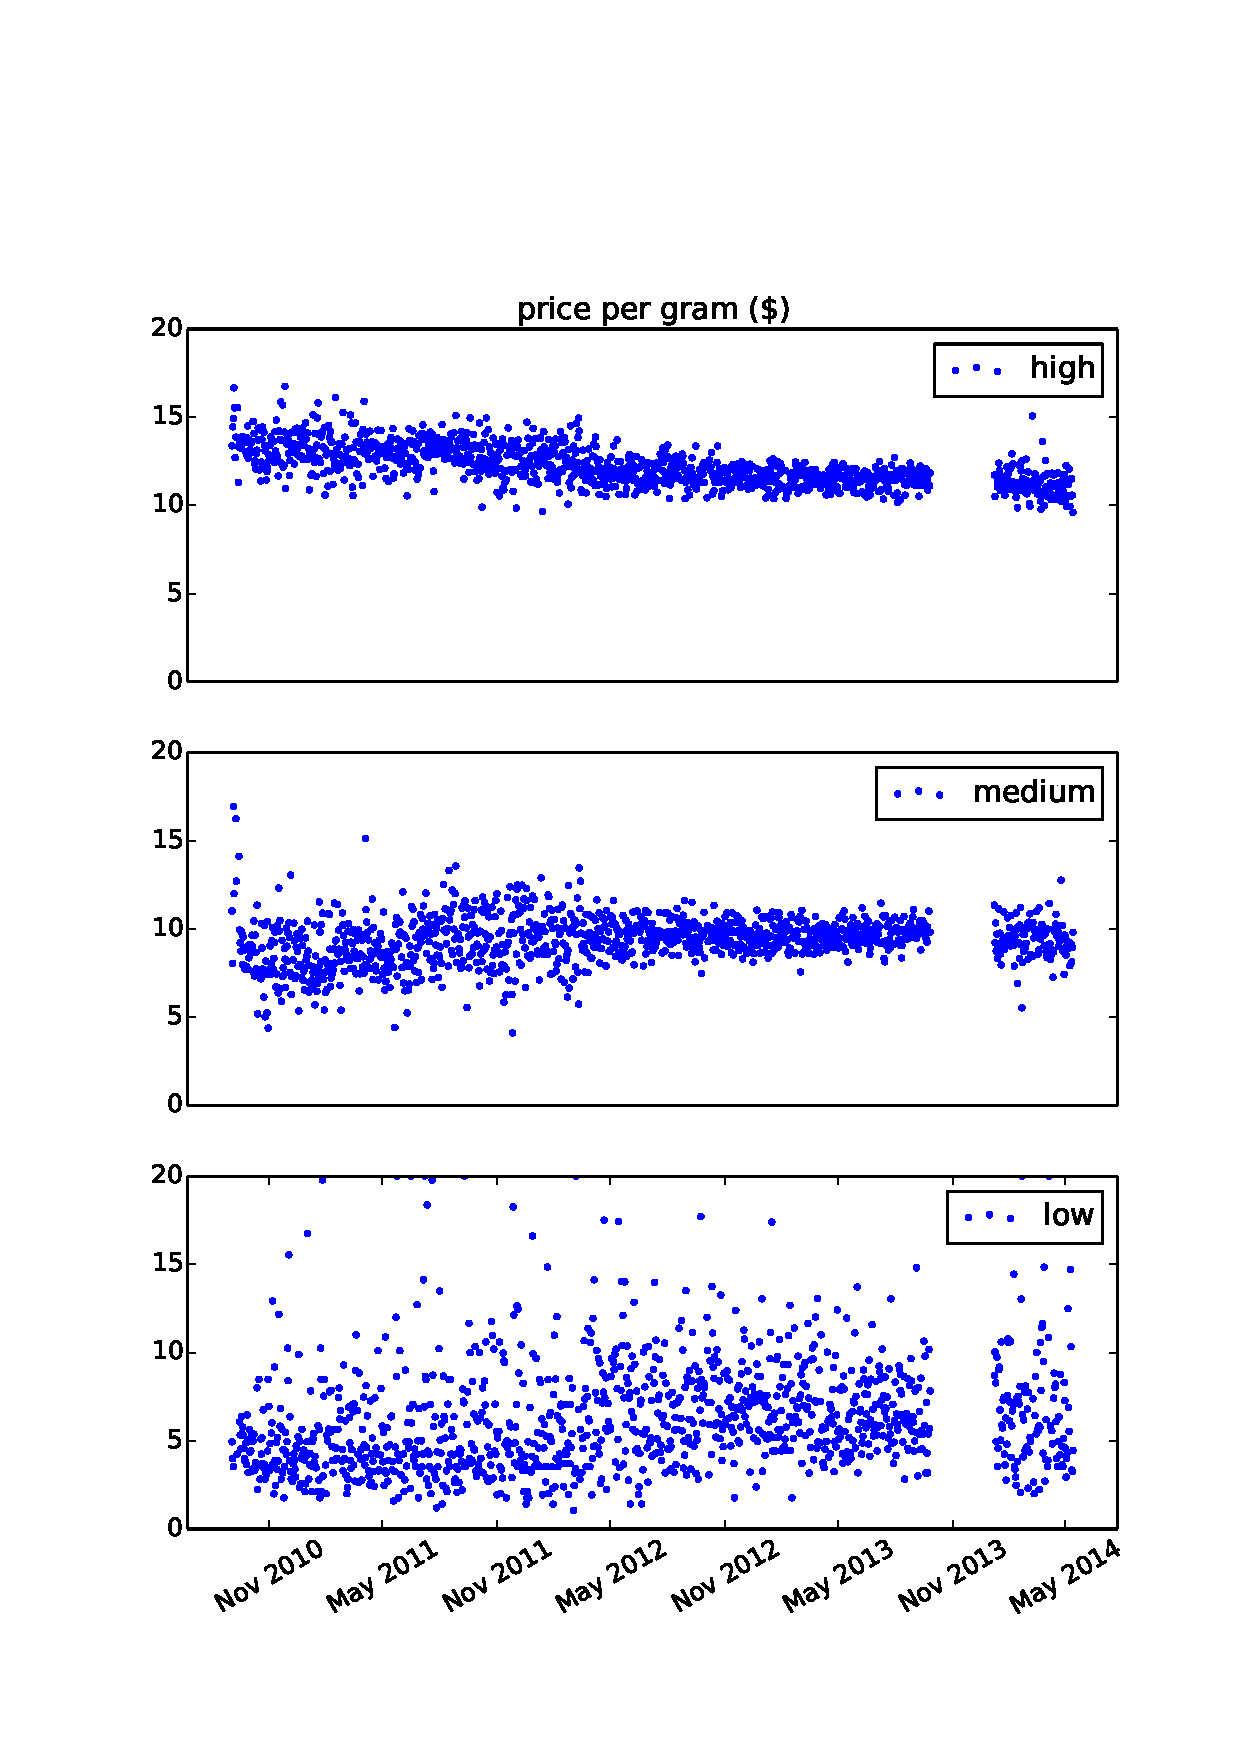
\includegraphics[width=3.5in]{figs/timeseries1.pdf}}
\caption{고급, 중급, 저급 품질 대마초에 대한 그램당 일별 시계열 그림.}
\label{timeseries1}
\end{figure}

그림~\ref{timeseries1}에 결과가 나와있다.
이 플롯 그림을 통해서 한가지 명백한 특징은 2013년 11월 틈이 있다는 것이다.
데이터 수집이 이 기간동안 활발하지 못하거나, 데이터가 이용가능하지 않았다는 것도 가능하다. 나중에 결측 데이터를 처리하는 방법을 생각해볼 것이다.
\index{결측값 (missing values)}

시각적으로 고품질 대마초 가격이 이 기간동안 하락하는 것처럼 보인다. 저품질 대마초 가격은 상승하는 것처럼 보이지만, 식별하기는 어렵다. 왜냐하면 변동성이 더 크기 때문이다. 품질 데이터는 자발적으로 보고한 것으로 시간에 따른 경향에는 참여자가 어떻게 품질 라벨을 적용했는지에 대한변동이 반영된다는 것을 기억하라.
\index{가격 (price)}


\section{선형 회귀 (Linear regression)}
\label{timeregress}

시계열분석에 특화된 방법론이 있지만, 많은 문제에 대해서, 시작하기 좋은 단순한 방법은 선형 회귀같은 범용 도구를 적용해보는 것이다.
다음 함수는 일별 가격 정보 데이터프레임을 받아서, 최소제곱 적합을 계산한다. StatsModels에서 모형과 결과 객체를 반환한다.

\index{데이터프레임 (DataFrame)}
\index{StatsModels}
\index{선형 회귀 (linear regression)}

\begin{verbatim}
def RunLinearModel(daily):
    model = smf.ols('ppg ~ years', data=daily)
    results = model.fit()
    return model, results
\end{verbatim}

그리고 나서, 수량을 반복하고 각각 모형에 적합한다.

\begin{verbatim}
    for name, daily in dailies.items():
        model, results = RunLinearModel(daily)
        print(name)
        regression.SummarizeResults(results)
\end{verbatim}

다음에 결과가 나와있다.

\begin{center}
\begin{tabular}{|l|l|l|c|} \hline
quality & intercept & slope & $R^2$ \\ \hline
high    & 13.450  & -0.708  & 0.444 \\
medium  &  8.879  & 0.283   & 0.050 \\
low     &  5.362  & 0.568   & 0.030 \\
\hline
\end{tabular}
\end{center}

추정된 기울기는 고품질 대마초 가격이 관측구간에서 매년 약 71 센트 하락했다; 중간 품질 대마초에 대해서는 매년 약 28 센트 층가했고, 저급 품질 대마초에 대해서는 매년 약 57 센트 증가했다. 이러한 추정값은 매우 작은 p-값으로 모두 통계적으로 유의하다.

\index{p-값 (p-value)}
  \index{유의성 (significant)} 
  \index{통계적 유의성 (statistically significant)}

고품질 대마초에 대한 $R^2$ 값은 0.44로 설명변수로서 시간이 관측된 가격 변동성의 44\%를 설명한다.
다른 대마초 품질에 대해서는 가격 변동이 더 작고, 가격에 변동성이 더 커서, $R^2$ 값이 더 작다(하지만, 여전히 통계적 유의성이 있다.)
\index{설명 변수 (explanatory variable)}
  \index{통계적 유의성 (statistically significant)}

다음 코드는 관측 가격과 적합값(fitted value)을 플롯으로 그린다.

\begin{verbatim}
def PlotFittedValues(model, results, label=''):
    years = model.exog[:,1]
    values = model.endog
    thinkplot.Scatter(years, values, s=15, label=label)
    thinkplot.Plot(years, results.fittedvalues, label='model')
\end{verbatim}

~\ref{implementation} 절에서 보았듯이, {\tt model}에는 {\tt exog}, {\tt endog}, 넘파이(NumPy)배열이 외생(설명), 내생(종속) 변수로 포함된다.
\index{넘파이 (NumPy)}
\index{설명변수 (explanatory variable)}
\index{종속변수 (dependent variable)}
\index{외생변수 (exogenous variable)}
\index{내생변수 (endogenous variable)}

\begin{figure}
% timeseries.py
\centerline{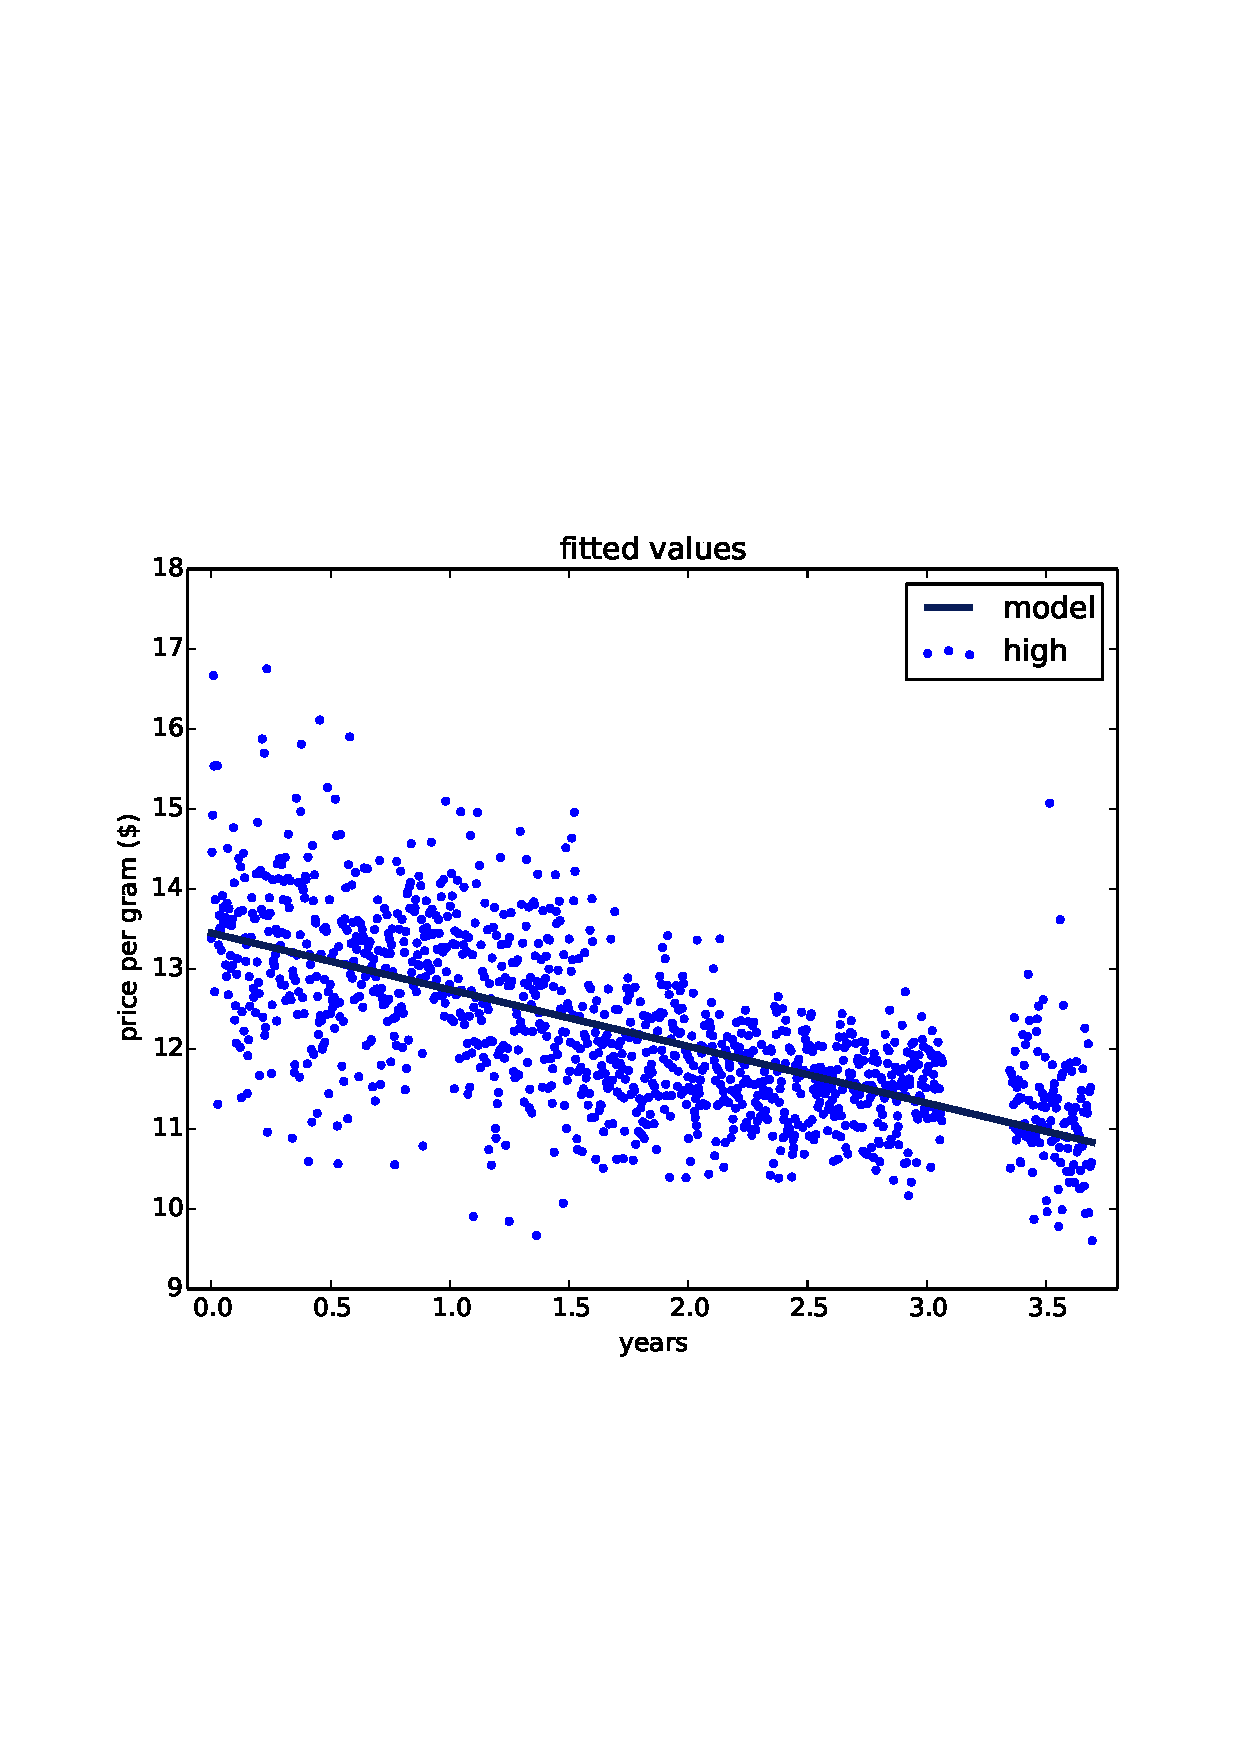
\includegraphics[height=2.5in]{figs/timeseries2.pdf}}
\caption{고급 대마초에 대한 그램당 일별가격 시계열과 선형 최소자승적합.}
\label{timeseries2}
\end{figure}

{\tt PlotFittedValues}은 데이터 점을 산점도로, 적합값을 선형 플롯 그림으로 만든다. 그림~\ref{timeseries2}에는 고품질 대마초에 대해 플롯을 그린 결과가 있다. 모형이 데이터에 대한 좋은 선형 적합처럼 보인다; 하지만, 선형회귀는 이러한 데이터에 대해서 가장 적절한 선택은 아니다.
\index{모형 (model)}
\index{적합값 (fitted values)}

\begin{itemize}

\item 첫째로, 장기 추세를 선형 혹은 다른 간단한 함수로 예측할 이유가 없다.
일반적으로, 가격은 수요와 공급에 의해 결정된다. 모두 시간에 따라 예측불가한 방향으로 변화한다.
\index{추세 (trend)}

\item 둘째, 선형회귀모형은 모든 데이터 (최근 혹은 과거)에 대해 동일한 가중치를 둔다. 예측 목적으로, 아마도 최근 데이터에 더 많은 가중치를 두어야 한다.
\index{가중치 (weight)}

\item 마지막으로, 선형회귀 가정중의 하나는 잔차가 상관되지 않는 잡음이라는 것이다. 시계열 데이터에서 연속된 값이 상관되기 때문에 종종 이런 가정은 틀리다. 
\index{잔차 (residuals)}

\end{itemize}

다음 절에서 대안을 제시하는 시계열 데이터에 대해서 더 적절하다.

\section{이동 평균 (Moving averages)}

대부분 시계열 분석은 관측된 계열이 다음 세가지 요소 합이라는 모형화 가정에 기반한다.

\index{모형 (model)}
\index{이동 평균 (moving average)}

\begin{itemize}

\item 추세 (Trend): 지속되는 변경사항을 잡아내는 평활 함수 (smooth function).
\index{추세 (trend)}

\item 계절성 (Seasonality): 주기적 변동, 아마도 일별, 주별, 월별, 혹은 년별 사이클.
\index{계절성 (seasonality)}

\item 잡음 (Noise): 장기 추세 주위 확률 변동.
\index{잡음 (noise)}

\end{itemize}

앞절에서 살펴봤듯이, 회귀는 계열에서 추세를 뽑아내는 한 방법이다. 하지만, 추세는 단순한 함수가 아니다. 훌륭한 대안은 {\bf 이동평균(moving average)}이다. 이동평균은 계열을 {\bf 윈도우(windows)}로 불리는 겹치지 않는 지역으로 나누고 각 윈도우에 있는 값을 평균낸다.
\index{윈도우 (window)}

가장 단순한 이동평균 중의 하나는 {\bf 이동평균 (rolling mean)}이다. 각 윈도우에 있는 값을 평균낸다. 예를 들어, 만약 윈도우 크기가 3이라면, 이동 평균은 0에서 2까지, 1에서 3까지, 2에서 4까지 등등 사이에 있는 값을 평균낸다.

\index{이동평균 (rolling mean)}
\index{평균 (mean)!이동 (rolling)}

판다스는에는 \verb"rolling_mean"가 있는데, 시리즈와 윈도우 크기를 인자로 받아 새로운 시리즈를 반환한다.
\index{판다스 (pandas)}
\index{시리즈 (Series)}

\begin{verbatim}
>>> series = np.arange(10)
array([0, 1, 2, 3, 4, 5, 6, 7, 8, 9])

>>> pandas.rolling_mean(series, 3)
array([ nan,  nan,   1,   2,   3,   4,   5,   6,   7,   8])
\end{verbatim}

첫 두값은 {\tt nan}이다; 다음 값은 첫 세 요소(0,1,2) 평균이다.
다음 값은 1,2,3의 평균. 등등

대마초 데이터에 \verb"rolling_mean"을 적용하기 전에, 결측값을 다루어야 한다. 하나 혹은 그 이상 대마초 품질 범주에 대해서, 관측 구간에 보고되지 않은 거래가 있는 몇일이 있고 데이터 수집이 활성화되지 않은 2013년 특정 기간이 있다.

\index{결측값 (missing values)}

지금까지 사용한 데이터프레임에 상기 날짜는 비워져있다; 인덱스는 데이터에 없는 날은 건너뛴다. 다음 분석에 대해서, 결측 데이터를 명시적으로 표기할 필요가 있다. 데이터프레임을 ``다시 인덱싱(reindexing)''해서 이 작업을 수행한다.
 \index{데이터프레임 (DataFrame)}
\index{reindex}

\begin{verbatim}
    dates = pandas.date_range(daily.index.min(), daily.index.max())
    reindexed = daily.reindex(dates)
\end{verbatim}

첫번째 행은 관측 구간 처음부터 끝까지 모든 날을 포함하는 날짜 범위를 계산한다. 두번째 행은 {\tt daily}로부터 모든 데이터를 갖는 새로운 데이터프레임을 생성하지만, {\tt nan}으로 채워진 모든 날째 행 열을 포함한다.

\index{구간 (interval)}
\index{날짜 범위 (date range)}

이제, 다음과 같이 이동평균 플롯을 그릴 수 있다.

\begin{verbatim}
    roll_mean = pandas.rolling_mean(reindexed.ppg, 30)
    thinkplot.Plot(roll_mean.index, roll_mean)
\end{verbatim}

윈도우 크기는 30이고, \verb"roll_mean"에 있는 각 값은 {\tt reindexed.ppg}으로부터 30 개값의 평균이다.

\index{판다스 (pandas)}
\index{윈도우 (window)}

\begin{figure}
% timeseries.py
\centerline{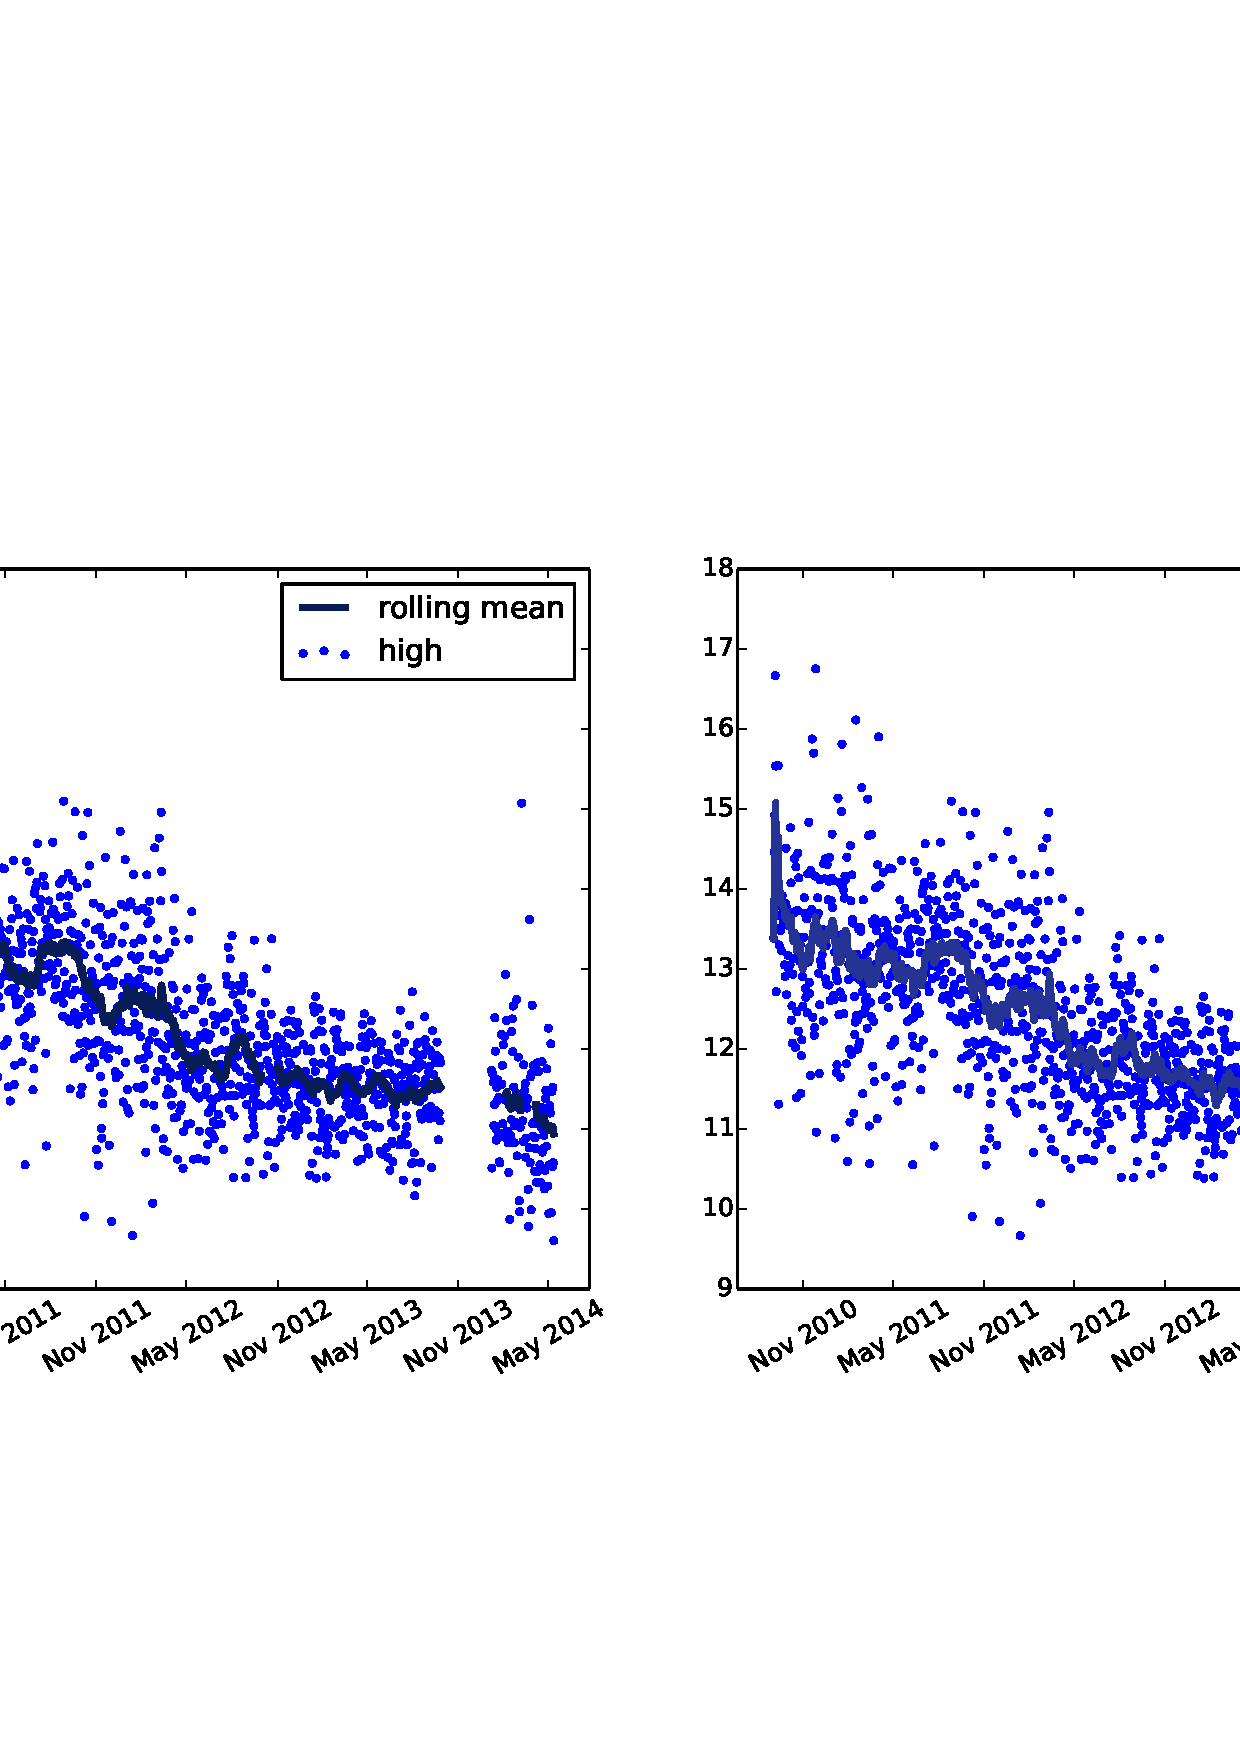
\includegraphics[height=2.5in]{figs/timeseries10.pdf}}
\caption{일별가격과 이동평균(좌측), 지수가중이동평균(exponentially-weighted moving average, EWMA, 우측).}
\label{timeseries10}
\end{figure}

그림~\ref{timeseries10} (왼편)에 결과가 그려져 있다.
이동평균은 잡음을 평활하고 추세를 추출하는 작업을 잘 하는 것처럼 보인다. 
첫 29개 값은 {\tt nan} 이고, 결측값이 있는 곳에, 또다른 {\tt nan} 29개가 다음에 있다. 이런 틈을 매울 수 있는 방법이 몇개 있지만, 성가신 작은 일이다.
\index{결측값 (missing values)}
\index{잡음 (noise)}
\index{평활 (smoothing)}

대안은 {\bf 지수가중 이동평균 (exponentially-weighted moving average)}으로 두가지 장점이 있다. 첫째, 이름에서 암시하듯이, 가중평균을 계산하는데 가장 최근 값에 가장 높은 가중치를 두고 이전 값의 가중치는 지수적으로 하락한다. 두번째, EWMA 판다스 구현이 결측값을 더 잘 처리한다.
\index{reindex}
\index{지수가중 이동평균 (exponentially-weighted moving average)}
\index{EWMA}

\begin{verbatim}
    ewma = pandas.ewma(reindexed.ppg, span=30)
    thinkplot.Plot(ewma.index, ewma)
\end{verbatim}

{\bf span} 모수는 대략 이동평균 윈도우 크기에 상응한다; 가중치가 얼마나 빨리 감쇄하는지 제어한다. 그래서 각 평균값에 무시못할 기여를 하는 점의 갯수를 결정한다.
\index{span}
\index{윈도우 (window)}

그림~\ref{timeseries10} (오른편)에 동일한 데이터에 대한 EWMA가 그려져 있다. 둘다 정의된 지점에서는 이동평균과 비슷하다. 하지만, 결측값이 없는데 작업하기 더 수월하게 한다. 시계열 시작부근에서 값들이 잡음이 있어 보이는데, 좀더 적은 데이터 점에 모형이 기반하기 때문이다.
\index{결측값 (missing values)}


\section{결측값 (Missing values)}

시계열 데이터 추세를 특성화했기 때문에, 다음 단계는 주기적인 행동인 계절성을 조사할 것이다. 인간 행동에 기반한 시계열 데이터는 종종 일별, 주별, 월별, 년별 주기(cycle)를 나타낸다. 다음 절에서, 계절성을 검정하는 방법을 제시한다. 하지만, 결측값에는 잘 동작하지 않는다. 그래서, 이 문제를 먼저 해결해야 한다.

\index{결측값 (missing values)}
\index{계절성 (seasonality)}

결측값을 채우는 간단하고 흔한 방법이 이동평균이다.
시리즈 메쏘드 {\tt fillna}가 원하는 것이다.

\index{시리즈 (Series)}
\index{fillna}

\begin{verbatim}
    reindexed.ppg.fillna(ewma, inplace=True)
\end{verbatim}

{\tt reindexed.ppg}에 {\tt nan}가 있는 곳 어디에서나, {\tt fillna}가 결측값을 {\tt ewma}에서 상응하는 값으로 교체한다. {\tt inplace} 옵션 플래그(flag)는 {\tt fillna}에 새로 생성하는 대신에 기존 시리즈를 변경하게 한다.

이 방식의 결점은 시리즈에 잡음(noise)을 과소추정하는 것이다. 재표본추출된 잔차(resampled residual)를 추가해서 이 문제를 해결할 수 있다.

\index{재표본추출 (resampling)}
\index{잡음 (noise)}

\begin{verbatim}
    resid = (reindexed.ppg - ewma).dropna()
    fake_data = ewma + thinkstats2.Resample(resid, len(reindexed))
    reindexed.ppg.fillna(fake_data, inplace=True)
\end{verbatim}

% (One note on vocabulary: in this book I am using
%``resampling'' in the statistical sense, which is drawing a random
%sample from a population that is, itself, a sample.  In the context
%of time series analysis, it has another meaning: changing the
%time between measurements in a series.  I don't use the second
%meaning in this book, but you might encounter it.)

{\tt resid}에는 {\tt ppg}가 {\tt nan}일 때 포함되지 않은 날 잔차값이 포함되어있다. \verb"fake_data"에는 이동평균 합과 잔차 확률표본(random sample)이 담겨있다. 마지막으로, {\tt fillna}는 {\tt nan}를 \verb"fake_data" 값으로 바꾼다.
\index{dropna}
\index{fillna}
\index{NaN}

\begin{figure}
% timeseries.py
\centerline{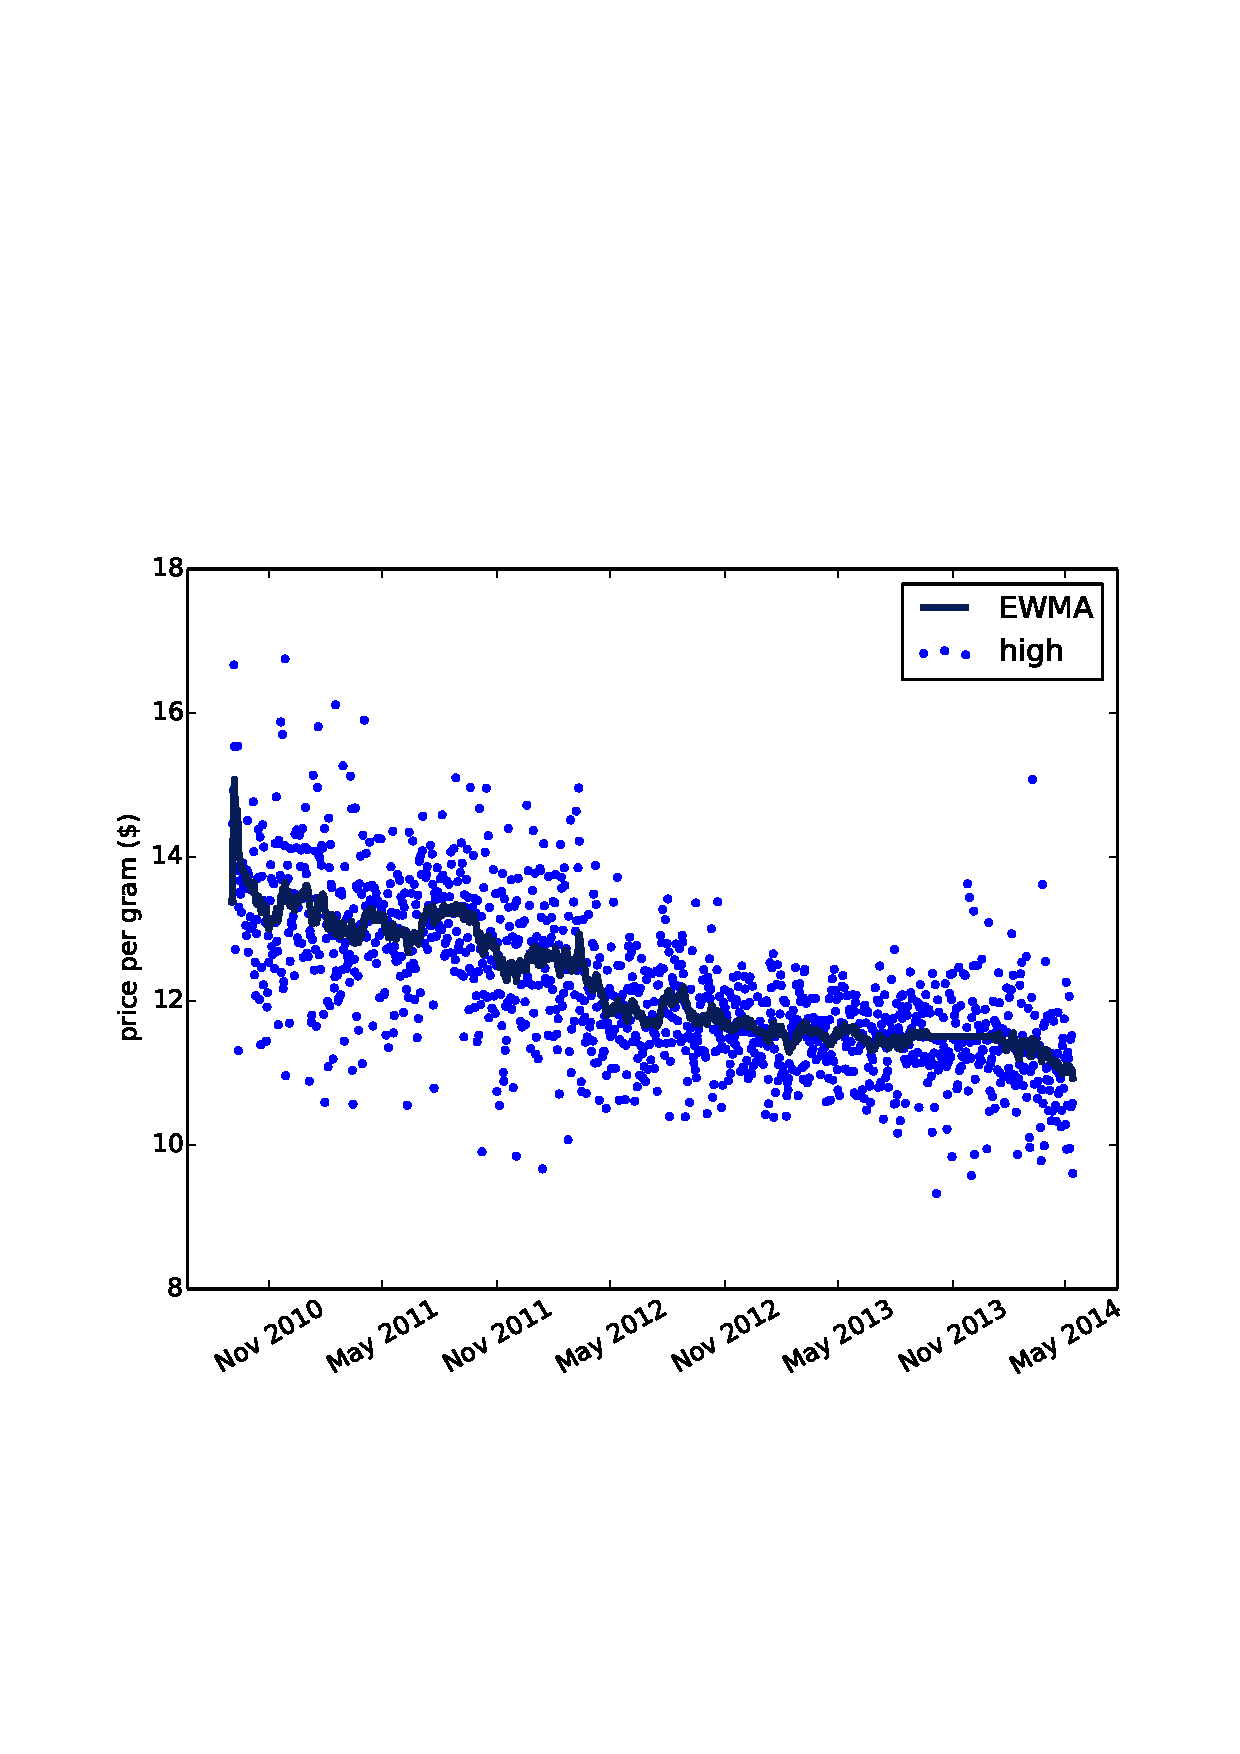
\includegraphics[height=2.5in]{figs/timeseries8.pdf}}
\caption{결측값을 채운 일별 가격.}
\label{timeseries8}
\end{figure}

그림~\ref{timeseries8}에 결과가 나와있다.
채워진 데이터는 시각적으로 실제값과 비슷하다.
재표본추출한 잔차가 랜덤(random)으로 결과는 매번 달라진다; 나중에,
결측값에서 생성된 오차를 어떻게 특성화하는지 살펴볼 것이다.

\index{재표본추출 (resampling)}
\index{결측값 (missing values)}


\section{계열 상관 (Serial correlation)}

가격은 매일 매일 변화하는데, 패턴을 보고 싶을지 모른다.
만약 월요일에 가격이 높다면, 다음 몇일동안 가격이 높을 것을 예상할 수 있다; 그리고, 만약 낮다면, 낮게 유지될 것을 예상할 수 있다.
이와 같은 패턴이 {\bf 계열 상관 (serial correlation)}이라고 부른다. 왜냐하면 각 값이 계열에 다음 값과 상관되기 때문이다.
\index{상관 (correlation)!계열 (serial)}
\index{계열 상관 (serial correlation)}

계열 상관을 계산하기 위해서, 시계열을 {\bf 시차(lag)}로 불리는 구간만큼 이동할 수 있다. 그리고 나서, 원시계열과 이동된 시계열 사이 상관을 계산한다.
\index{시차 (lag)}

\begin{verbatim}
def SerialCorr(series, lag=1):
    xs = series[lag:]
    ys = series.shift(lag)[lag:]
    corr = thinkstats2.Corr(xs, ys)
    return corr
\end{verbatim}

이동한 후에, 첫 {\tt 시차 (lag)} 값이 {\tt nan}이라, 슬라이스를 사용해서 {\tt Corr}를 계산하기 전에 제거한다.
\index{NaN}

%high 0.480121816154
%medium 0.164600078362
%low 0.103373620131

만약 {\tt SerialCorr}을 시차 1을 가진 원가격데이터에 적용하면, 계열상관이 고품질 대마초에 대해 0.48, 중간품질에는 0.16, 저품질에는 0.10이 된다.
장기 추세를 갖는 어떤 시계열에 대해서도, 강한 계열상관을 예상한다; 예를 들어, 만약 가격이 떨어지고 있다면, 계열 절반 전반부에는 평균보다 상위 값을, 계열 절반 후반부에는 평균보다 하위 값을 예상한다.

만약 추세를 제거한다면, 상관이 지속하는지 살펴보는 것이 더 흥미롭다.
예를 들어, EWMA 잔차를 계산하고 나서 계열 상관을 계산한다.
\index{EWMA}

\begin{verbatim}
    ewma = pandas.ewma(reindexed.ppg, span=30)
    resid = reindexed.ppg - ewma
    corr = SerialCorr(resid, 1)
\end{verbatim}

lag=1으로 추세 제거된 데이터에 대한 계열 상관은 고품질에는 -0.022,
중간품질에는 -0.015, 저품질에는 0.036이다.
계열 상관값이 작아서, 이 시계열 데이터에는 하루 계열상관이 매우 작거나 없다.
\index{판다스 (pandas)}

주별, 월별, 년별 계절성을 점검하기 위해서, 다시 다른 시차를 갖는 분석을 실행한다. 다음에 결과가 나와있다. 
\index{계절성 (seasonality)}

\begin{center}
\begin{tabular}{|c|c|c|c|}
\hline
lag & high & medium & low \\ \hline
1 & -0.029 & -0.014 & 0.034 \\
7 & 0.02 & -0.042 & -0.0097 \\
30 & 0.014 & -0.0064 & -0.013 \\
365 & 0.045 & 0.015 & 0.033 \\
\hline
\end{tabular}
\end{center}

다음절에서, 이러한 상관이 통계적 유의성(통계적 유의성은 없다)이 있는지 검정할 것이다. 하지만, 이 지점에서 잠정적으로 이들 시계열 데이터에 상당한 계절적 패턴이, 적어도 이런 시차에는 없다고 결론내릴 수 있다.

\index{유의성 (significant)} 
\index{통계적 유의성 (statistically significant)}


\section{자기상관 (Autocorrelation)}

만약 시계열이 계열상관을 갖고 있다고 생각하지만 어떤 시차를 검정할지 모른다면, 모든 시차를 검정할 수 있다!!! {\bf 자기상관 함수 (autocorrelation function)}는 시차에서 주어진 시차를 갖는 계열 상관에 매핑하는 함수다. ``자기상관(Autocorrelation)''은 계열상관의 또 다른 이름으로, 시차가 1이 아닐 때 더 많이 사용된다.
\index{자기상관 함수 (autocorrelation function)}

StatsModels는 ~\ref{statsmodels}절에 선형회귀에 사용했는데, 자기상관 함수를 계산하는 {\tt acf}를 포함하여 시계열분석에 함수도 제공한다.
\index{StatsModels}

\begin{verbatim}
    import statsmodels.tsa.stattools as smtsa
    acf = smtsa.acf(filled.resid, nlags=365, unbiased=True)
\end{verbatim}

{\tt acf}는 계열상관을 0 시차부터 {\tt nlags}까지 계산한다.
{\tt unbiased} 플래그옵션은 {\tt acf}에 표본크기에 대한 추정값을 보정하게 한다. 결과는 상관 배열이다. 만약 고품질 대마초에 대한 일별 가격을 선택하고, 1, 7, 30, 365 시차에 대한 상관을 추출한다면, 
{\tt acf}와 {\tt SerialCorr}는 근사적으로 거의 동일한 결과를 산출한다.
\index{acf}

\begin{verbatim}
>>> acf[0], acf[1], acf[7], acf[30], acf[365]
1.000, -0.029, 0.020, 0.014, 0.044
\end{verbatim}

{\tt lag=0}으로, {\tt acf} 본인과 계열 상관을 계산하는데, 항상 1 이다.
\index{시차 (lag)}

\begin{figure}
% timeseries.py
\centerline{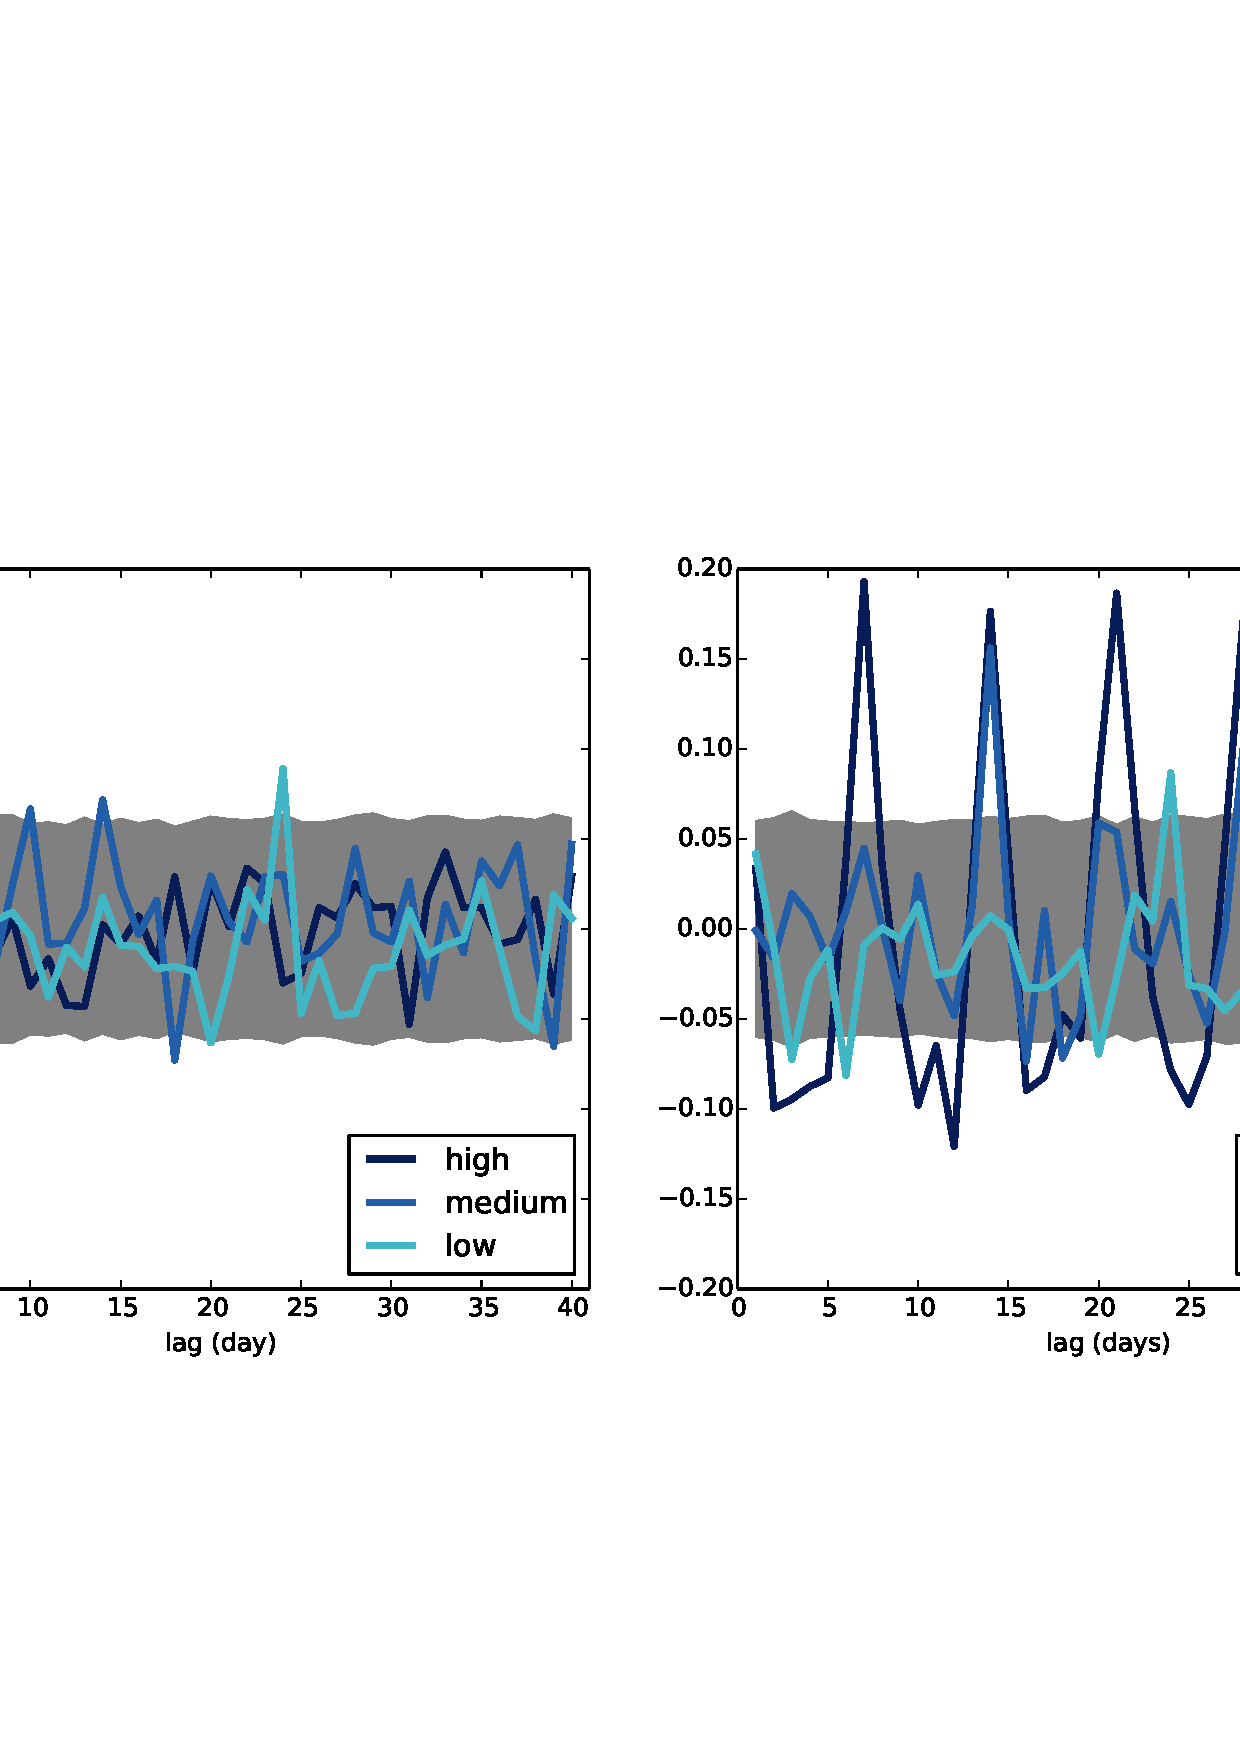
\includegraphics[height=2.5in]{figs/timeseries9.pdf}}
\caption{일별가격에 대한 자기상관 함수(좌측), 모의시험으로 주별 계절성을 갖는 일별가격에 대한 자기상관 함수(우측).}
\label{timeseries9}
\end{figure}

그림~\ref{timeseries9} (왼편)에는 {\tt nlags=40} 시차로 3개 품질 범주에 대한 자기상관함수를 보여준다.
회색지역에는 만약 실제 자기상관이 없다면 예상되는 정규 변동성이 나타나 있다; 이 범위 밖에 있는 어느 것이나 p-값이 5\%보다 작아서 통계적 유의성이 있다. 거짓양성(false positive)가 5\% 이고 120개 상관(3개 시계열에 대해서 시차 40)을 계산하기 때문에, 이 구역 박에 약 6개 점이 예상된다.
사실 7개 점이 있다. 이들 시계열에는 우연으로 설명될 수 없는 자기상관이 없다고 결론낸다.
\index{p-값 (p-value)}
  \index{유의성 (significant)} 
  \index{통계적 유의성 (statistically significant)}
\index{거짓양성 (false positive)}

잔차를 재표본추출해서 회식 지역을 계산했다. 코드는 {\tt timeseries.py} 파일에 있다; 함수는 {\tt SimulateAutocorrelation}다.
\index{재표본추출 (resampling)}

계절적 성분이 있을 때, 자기상관 함수가 어떤 느낌인지 살펴보기 위해서, 주별 주기를 더해서 모의 시험 데이터를 생성했다. 대마초 수요가 주말에 더 높다고 가정하면, 가격이 더 높을 것으로 예상할 수 있다. 효과를 모의 시험하기 위해서, 금요일 혹은 토요일 날짜를 선택하고, 가격에 \$0 에서 \$2 까지 균등분포에서 추출한 임의 금액을 더한다.
\index{모의시험 (simulation)}
\index{균등 분포 (uniform distribution)}
\index{분포 (distribution)!균등 (uniform)}

\begin{verbatim}
def AddWeeklySeasonality(daily):
    frisat = (daily.index.dayofweek==4) | (daily.index.dayofweek==5)
    fake = daily.copy()
    fake.ppg[frisat] += np.random.uniform(0, 2, frisat.sum())
    return fake
\end{verbatim}

{\tt frisat}는 부울 시리즈로, 만약 여일이 금요일 혹은 토요일이면, {\tt 참(True)}이다. {\tt fake}는 새 데이터프레임으로 원래 {\tt daily} 복사본으로 {\tt ppg}에 확률값(random value)을 더해서 변경한다. {\tt frisat.sum()}은 금요일과 토요일 전체 갯수로 생성해야하는 확률값 갯수가 된다.
\index{데이터프레임 (DataFrame)}
\index{시리즈 (Series)}
\index{부울 (boolean)}


그림~\ref{timeseries9} (오른편)에는 모의시험 계절성을 갖는 가격에 대한 자기상관 함수가 나타나 있다. 예상했듯이, 시차가 7의 곱이 될 때 가장 높다. 고급과 중급 품질에 대해 신규 상관이 통계적 유의성이 있다. 저급 품질에 대서는 유의적이지 않은데 이유는 이 범주에 잔차가 크기 때문이다; 잡음을 뚫고 보여지기 위해서는 효과가 더 커야한다.
\index{유의성 (significant)} \index{통계적 유의성 (statistically significant)}
\index{잔차 (residuals)}
\index{시차 (lag)}


\section{예측 (Prediction)}  

시계열 분석은 시간에 변화하는 시스템 행동을 조사하고 때때로 설명하는데 사용될 수 있다. 또한 예측도 할 수 있다.
\index{예측 (prediction)}

~\ref{timeregress}절에서 사용한 선형회귀는 예측에 사용될 수 있다.
RegressionResults 클래스에 {\tt predict}를 사용해서
설명변수를 포함하는 데이터프레임을 인자로 받아 예측 시퀀스를 반환한다.
다음에 코드가 있다.
\index{설명변수 (explanatory variable)}
\index{선형회귀 (linear regression)}

\begin{verbatim}
def GenerateSimplePrediction(results, years):
    n = len(years)
    inter = np.ones(n)
    d = dict(Intercept=inter, years=years)
    predict_df = pandas.DataFrame(d)
    predict = results.predict(predict_df)
    return predict
\end{verbatim}

{\tt results}는 RegressionResults 객체다; 
{\tt years}는 예측하려는 시간 값 시퀀스다.
함수가 데이터프레임을 생성하고 {\tt predict}에 전달하고 결과를 반환한다.
\index{판다스 (pandas)}
\index{데이터프레임 (DataFrame)}

만약 원하는 모든 것이, 하나의 최선을 다한 예측이라면, 완료했다.
하지만, 대부분 목적에 대해서, 오차를 정량화하는 것이 중요하다.
다른 말로, 예측이 얼마의 정확성이 있는지 알고싶다.

고려해야 하는 오류 원천이 3가지 있다.

\begin{itemize}

\item 표집오차 (Sampling error): 
예측은 추정 모수에 기반하는데, 추정 모수는 표본 확률변동에 의존한다.
만약 실험을 다시 실시한다면, 추정값이 변화할 것으로 예상된다.
\index{표집오차 (sampling error)}
\index{모수 (parameter)}

\item 확률변동 (Random variation):
설사 추정 모수가 완벽할지라도, 관측 데이터는 장기추세주변에서 확률적으로 변동하고 이러한 변동은 미래에도 계속될 것으로 예상된다.
\index{잡음 (noise)}

\item 모형화 오차 (Modeling error): 
장기 추세가 선형이 아니라는 증거를 이미 봤다. 그래서 선형 모형에 기반한 예측은 결국 실패할 것이다.
\index{모형화 오차 (modeling error)}

\end{itemize}

고려할 또 다른 오류 원천은 예상치 못한 미래 사건이다. 
농산물 가격은 날씨에 영향을 받고, 모든 가격은 정치와 법에 영향하에 있다. 이 책을 집필하고 있을 때, 대마초는 미국 두주에서 합법이고, 의료목적으로 20개 이상 주에서 합법이다. 만약 더 많은 주가 합법화한다면, 가격은 내려갈 것이다. 하지만, 연방정부가 단속한다면, 가격이 치솟을지 모른다.

모형화 오차 (modeling error)와 예상치 못한 미래 사건은 정량화하기 어렵니다. 표집오차와 확률변동은 다루기 더 쉽다. 그래서 먼저 이것을 다뤄보자.

표집오차를 정량화하기 위해서, ~\ref{regest}절에서 했던 것처럼 재표본추출법을 사용한다. 늘 그렇듯이, 목적은 만약 실험을 다시 실행한다면 무엇이 발생할 것인지 모의 시험하는데 실제 관측점을 사용하는 것이다.
모의시험은 추정 모수가 맞지만 확률 잔차가 다를 수 있다는 가정에 기반한다.
여기 모의 시험을 수행하는 함수가 있다.
\index{재표본추출 (resampling)}

\begin{verbatim}
def SimulateResults(daily, iters=101):
    model, results = RunLinearModel(daily)
    fake = daily.copy()
    
    result_seq = []
    for i in range(iters):
        fake.ppg = results.fittedvalues + Resample(results.resid)
        _, fake_results = RunLinearModel(fake)
        result_seq.append(fake_results)

    return result_seq
\end{verbatim}

{\tt daily}는 관측 가격을 포함하는 데이터프레임이다;
{\tt iters}는 모의 시험할 횟수다.
\index{데이터프레임 (DataFrame)}
\index{가격 (price)}

{\tt SimulateResults}는 ~\ref{timeregress}절로부터 {\tt RunLinearModel}을 사용해서 관측값의 기울기와 절편을 추정한다.

루프를 반복할 때마다, 잔차를 재표본추출하고 적합값에 더해서 ``fake'' 데이터셋을 생성한다. 그리고 나서, ``fake'' 데이터에 선형모형을 실행하고 RegressionResults 객체에 저장한다.
\index{모형 (model)}
\index{잔차 (residuals)}

다음 단계로 예측을 생성하는데 모의 시험 결과를 사용한다.

\begin{verbatim}
def GeneratePredictions(result_seq, years, add_resid=False):
    n = len(years)
    d = dict(Intercept=np.ones(n), years=years, years2=years**2)
    predict_df = pandas.DataFrame(d)
    
    predict_seq = []
    for fake_results in result_seq:
        predict = fake_results.predict(predict_df)
        if add_resid:
            predict += thinkstats2.Resample(fake_results.resid, n)
        predict_seq.append(predict)

    return predict_seq
\end{verbatim}

{\tt GeneratePredictions}는 이전 단계에서 결과 시퀀스 뿐만 아니라 
예측을 생성할 구간을 명시하는 부동소수점 시퀀스 {\tt years}, 그리고 재표본추출 잔차가 직선 예측에 추가해야 하는지를 말지를 나타내는 \verb"add_resid"을 인자로 받는다.
{\tt GeneratePredictions}은 RegressionResults 시퀀스를 반복해서 예측 시퀀스를 생성한다.
\index{재표본추출 (resampling)}

\begin{figure}
% timeseries.py
\centerline{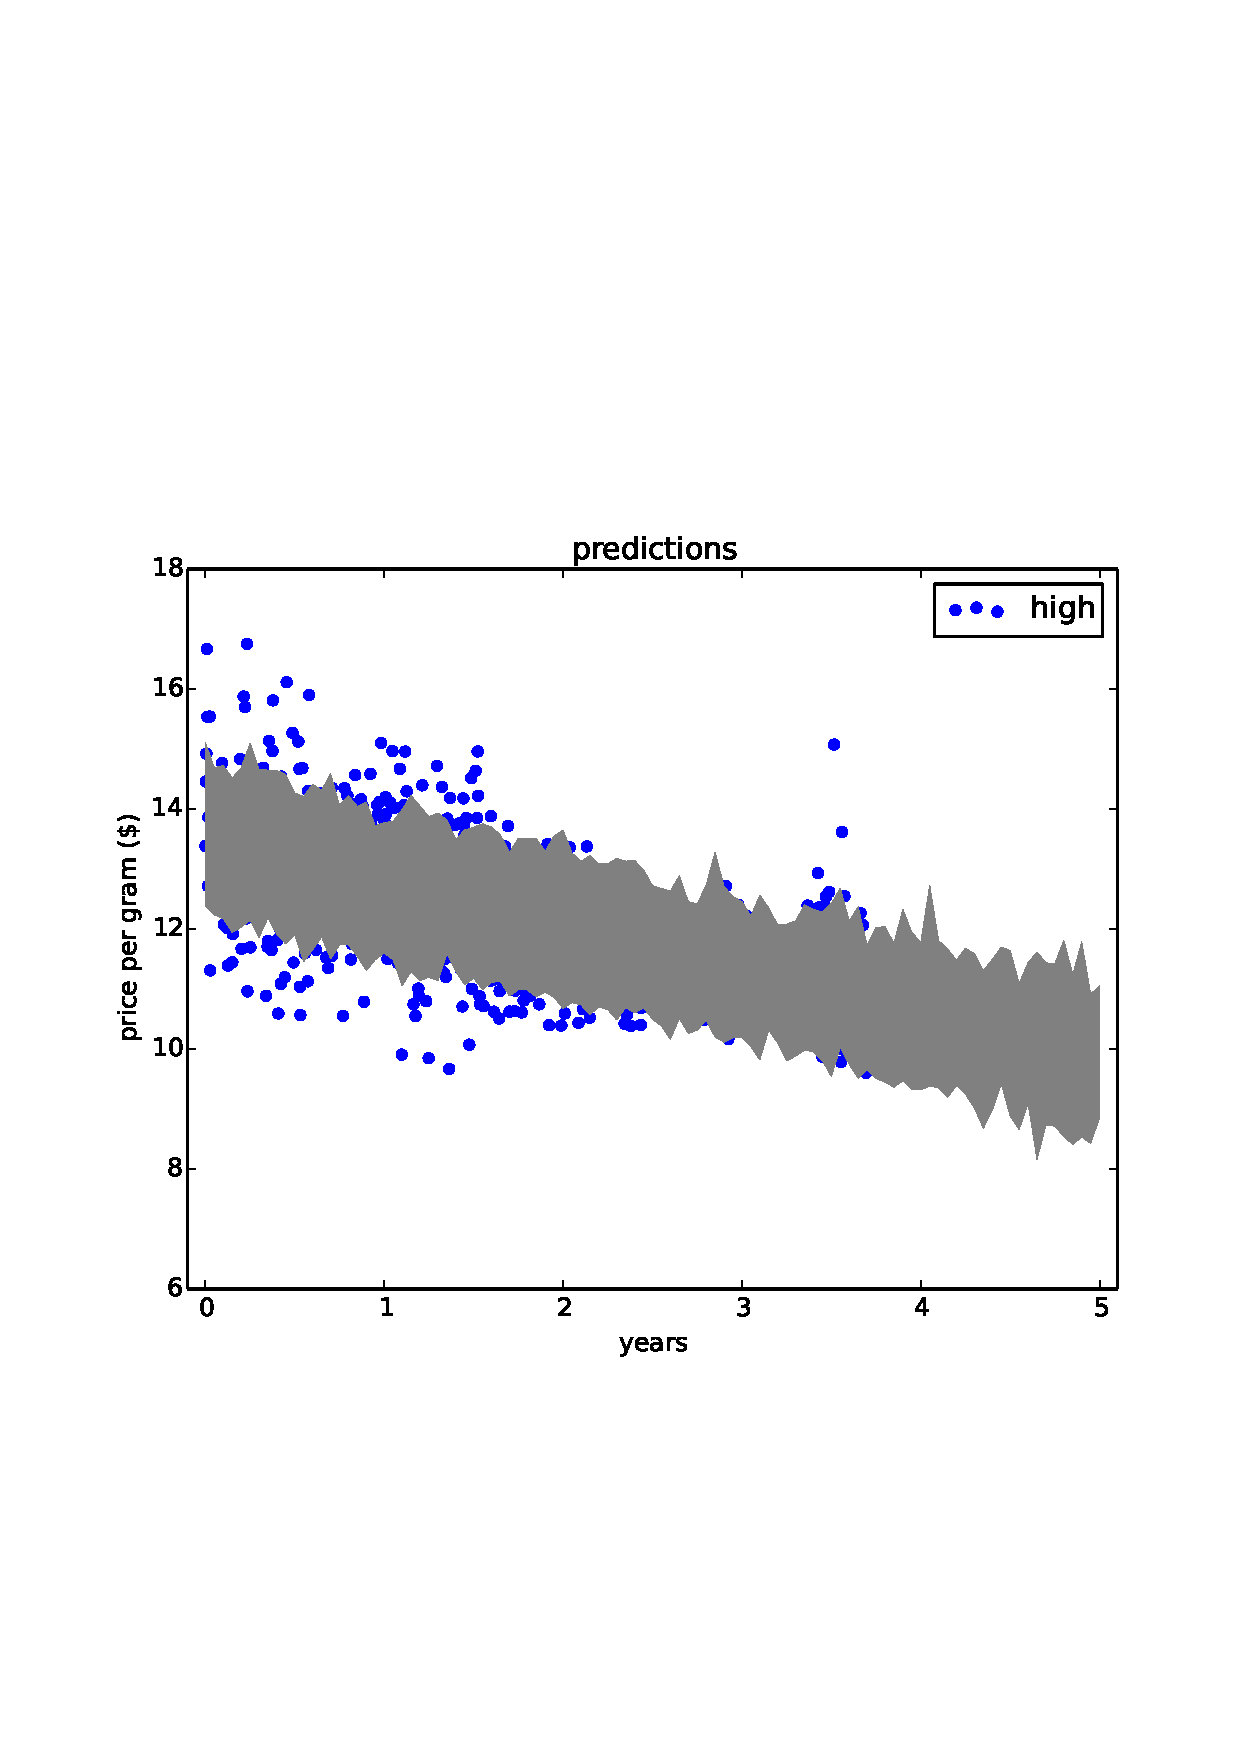
\includegraphics[height=2.5in]{figs/timeseries4.pdf}}
\caption{선형적합에 기초한 예측, 표집오차와 예측 오차에 기인한 변동성을 나타냄.}
\label{timeseries4}
\end{figure}

마지막으로, 다음에 예측으로 90\% 신뢰구간을 플롯으로 그리는 코드가 있다.
\index{신뢰구간 (confidence interval)}

\begin{verbatim}
def PlotPredictions(daily, years, iters=101, percent=90):
    result_seq = SimulateResults(daily, iters=iters)
    p = (100 - percent) / 2
    percents = p, 100-p

    predict_seq = GeneratePredictions(result_seq, years, True)
    low, high = thinkstats2.PercentileRows(predict_seq, percents)
    thinkplot.FillBetween(years, low, high, alpha=0.3, color='gray')

    predict_seq = GeneratePredictions(result_seq, years, False)
    low, high = thinkstats2.PercentileRows(predict_seq, percents)
    thinkplot.FillBetween(years, low, high, alpha=0.5, color='gray')
\end{verbatim}

{\tt PlotPredictions}이 {\tt GeneratePredictions}을 두번 호출한다; 한번은 \verb"add_resid=True"이고, 다른 한번은 \verb"add_resid=False"이다.
{\tt PercentileRows}를 사용해서 각 년도에 대해서 5번째와 95번째 백분위수를 선택한다. 그리고 나서, 경계 사이 회색지역을 플롯으로 그린다..
\index{FillBetween}

그림~\ref{timeseries4}에 결과가 나와 있다.
짙은 회색 지역이 표집오차에 대한 90\% 신뢰구간을 나타낸다; 즉,
표집때문에 추정 기울기와 절편에 대한 불확실성.
\index{표집오차 (sampling error)}

밝은 지역은 예측 오차에 대한 90\% 신뢰구간을 보여주는데,
표집오차와 확률변동 합이다.
\index{잡음 (noise)}

이들 지역이 표집오차, 확률변동을 정량화하지만, 모형화 오류는 정량화하지 않는다. 일반적으로 모형화 오류는 정량화하기 어렵다. 하지만, 이경우에 최소한 오차 원천 하나(예측치 못한 외부 사건)는 다룰 수 있다.
\index{모형화 오차 (modeling error)}

회귀 모형은 시스템이 정상성(stationary, 시불변)이 있다는 가정에 기반한다; 즉, 모형 모수는 시간에 따라 변하지 않는다.
좀더 구체적으로, 기울기와 절편 뿐만 아니라 잔차 분포도 일정하다고 가정한다.
\index{정상성 모형 (stationary model)}
\index{모수 (parameter)}

하지만, 그림~\ref{timeseries10}에 있는 이동 평균을 살펴보면, 최소한 관측 기간동안 한번 기울기는 변하고 잔차 분산이 후반부보다 전반부에서 더 큰 것처럼 보인다.
\index{기울기 (slope)}

결과로, 추정한 모수는 관측 기간에 의존성이 있다.
이것이 예측에 얼마나 많은 효과를 갖는지 살펴보기 위해서,
다른 시작과 종료 날짜를 갖는 관측 구간을 사용하도록 {\tt SimulateResults}를 연장한다.
구현은 {\tt timeseries.py} 파일에 있다.
\index{모의시험 (simulation)}

\begin{figure}
% timeseries.py
\centerline{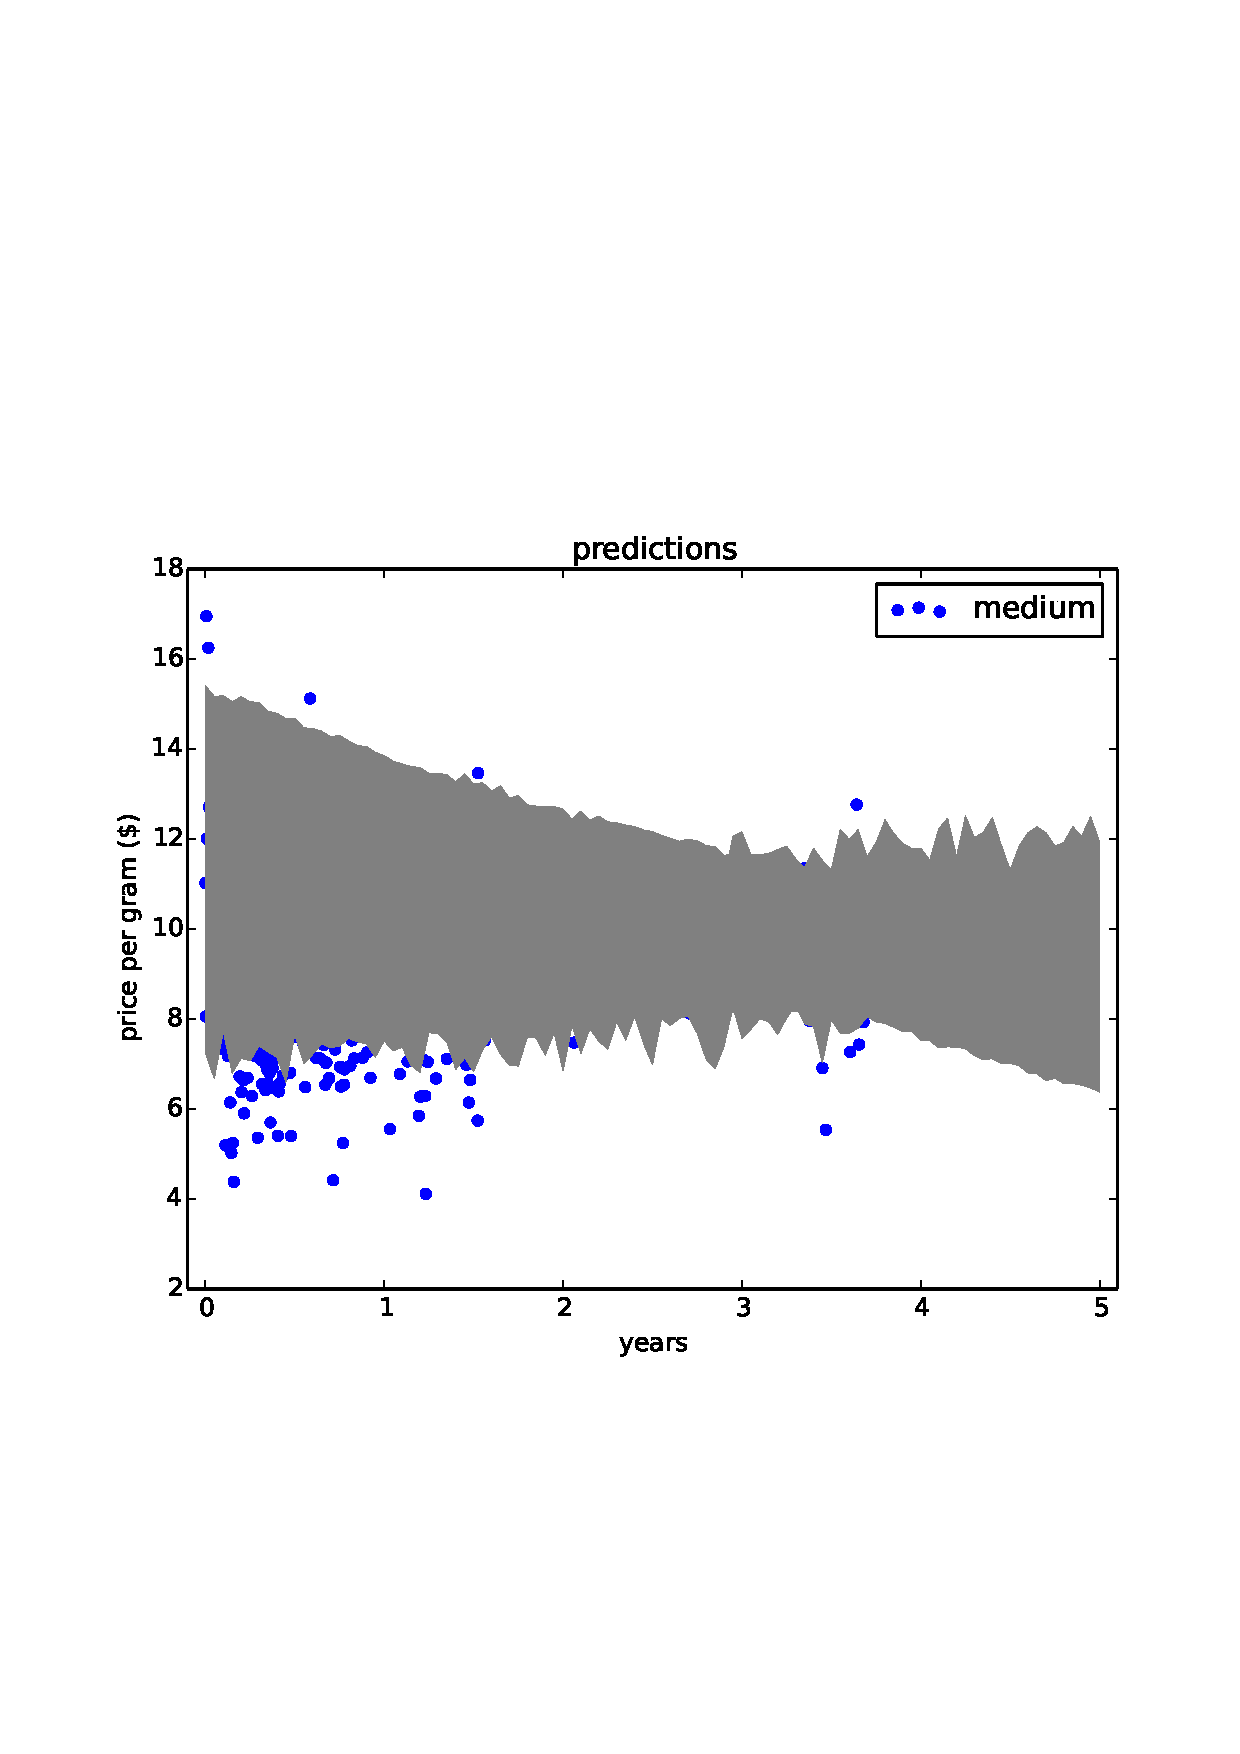
\includegraphics[height=2.5in]{figs/timeseries5.pdf}}
\caption{선형적합에 기초한 예측, 관측점 간격에 기인한 변동성을 나타냄.}
\label{timeseries5}
\end{figure}

그림~\ref{timeseries5}에 중간 품질 대마초에 대한 결과가 나와 있다.
옅은 회색 구역이 신뢰구간을 보여주는데 표집오차, 확률변동, 관측구간 변동으로 인한 불확실성이 포함한다.
\index{신뢰구간 (confidence interval)}
\index{구간 (interval)}

전체 구간에 기반한 모형이 양수 기울기를 갖고 있는데, 가격이 오르고 있다는 것을 나타낸다. 하지만, 가장 최신 구간은 하락하는 가격 신호를 보여준다. 
그래서 가장 최신 데이터에 기반한 모형은 음수 기울기를 갖는다.
결과로, 가장 폭이 넗은 구간은 내년에 하락하는 가격 가능성을 포함한다.
\index{모형 (model)}


\section{추가 읽기}
시계열 분석은 큰 주제다; 이번 장에서 단지 표면만 긁었을 뿐이다.
시계열 데이터로 작업하는데 중요한 도구는 자기회귀로 여기서는 다루지 않았다. 왜냐하면, 작업한 예제 데이터에 사용하기에 적합하지 않았기 때문이다.
\index{시계열 (time series)}

하지만, 이장에 있는 내용를 학습하면, 자기회귀를 학습할 준비가 된 것이다. 추천하는 한 교재는 Philipp Janert가 저술한 책, {\it Data Analysis with Open Source Tools} O'Reilly Media, 2011. 
시계열에 대한 장에서 여기서 다루지 않는 내용을 학습할 수 있다.
\index{Janert, Philipp}


\section{연습문제}

이 연습문제에 대한 저자 해답은 \verb"chap12soln.py"에 나와있다.

\begin{exercise}
이번 장에서 저자가 사용한 선형모형은 선형이라는 명백한 결점이 있고,
가격이 시간에 따라 선형으로 변할 것이라고 예측할 이유는 없다.
\ref{nonlinear}~절에서 했던 것처럼, 2차항을 추가해서 모형에 유연성을 더할 수 있다.

\index{비선형}
\index{선형 모형}
\index{2차 모형}

2차 모형을 사용해서 시계열 일별가격을 적합할 수 있고,
모형을 사용해서 예측값도 생성할 수 있다.
2차 모형을 돌리는 {\tt RunLinearModel} 버젼을 작성해야할 것이다.
하지만, 예측을 생성하는데 {\tt timeseries.py}에 나온 코드를 재사용할 수도 있다.

\index{예측}

\end{exercise}

\begin{exercise}

\ref{hypotest}~절에 나온 {\tt HypothesisTest}을 확장하는 
클래스를 정의하는데 명칭은 {\tt SerialCorrelationTest}이다.
데이터로 시계열과 시차(lag)를 받아서, 주어진 시차를 갖는 
시계열 데이터의 계열상관을 계산하고 나서,
관측된 상관에 대한 p-값을 계산한다.

\index{HypothesisTest}
\index{p-값}
\index{시차}

이 클래스를 사용해서 원가격 데이터에 나온 계열 상관이 통계적으로 유의적인지 검정한다.
또한, 선형모형과 (만약 이전 예제를 수행했다면) 2차 모형의 잔차를 검정한다.
\index{2차 모형}
  \index{유의적인} \index{통계적으로 유의한}

\end{exercise}

\begin{exercise}
예측을 만들어 내는데, EWMA 모형을 확장하는 몇가지 방식이 있다.
가장 단순한 방법중의 하나는 다음과 같다:
\index{EWMA}

\begin{enumerate}

\item 시계열 EWMA를 계산하고, 가장 마지막 점을 절편 {\tt inter}으로 사용한다.

\item 시계열의 연속 요소사이에 EWMA 차이를 계산하고, 가장 마지막 점을 기울기 {\tt slope}로 사용한다.
\index{기울기}

\item 미래 시점에 값을 예측하는데, {\tt inter + slope * dt}을 계산한다.
여기서 {\tt dt}는 예측 시점과 가장 마지막 예측 시점의 차이다.
\index{예측}

\end{enumerate}

이 방법을 사용해서, 마지막 관측점 다음 연도에 대한 예측을 생성한다.
몇가지 힌드는 다음과 같다:

\begin{itemize}

\item {\tt timeseries.FillMissing}을 사용해서 분석을 돌리기 전에 결측값을 채워넣는다.
이런 방식으로 연속된 요소값 사이 시점이 일치한다.
\index{결측값}

\item {\tt Series.diff}을 사용해서 연속된 요소 사이 차이를 계산한다.
\index{시리즈}

\item {\tt reindex}을 사용해서 데이터프레임을 미래로 연장한다.
\index{reindex}

\item {\tt fillna}을 사용해서 예측한 값을 데이터프레임에 넣는다.
\index{fillna}

\end{itemize}

\end{exercise}


\section{용어 사전}

\begin{itemize}

\item 시계열(time series): 각 값이 시간도장(timestamp)과 연관된 데이터셋. 종종 측정값과 추집된 시점 계열.
\index{시계열 (time series)}

\item 윈도우 (window): 이동 평균을 계산하는 종종 사용되는 시계열에 연속값 시퀀스.
\index{윈도우 (window)}

\item 이동평균 (moving average): 겹쳐지지 않는 일련의 윈도우에 대한 평균을 계산함으로써 시계열에 잠재하는 추세를 추정하는데 사용되는 여러 통계량 중의 하나.
\index{이동평균 (moving average)}

\item 이동평균 (rolling mean):각 윈도우 평균값에 기반한 이동평균.
\index{이동평균 (rolling mean)}

\item 지수가중이동평균 (exponentially-weighted moving average, EWMA): 
가중평균에 기반한 이동평균으로 가장 최근 값에 가장 높은 가중치를 두고, 이전 값에 대해서는 지수적으로 줄어드는 가중치를 둔다.
\index{지수가중이동평균 (exponentially-weighted moving average)}
\index{EWMA}

\item 스팬 (span): 가중치가 얼마나 빨리 줄어드는지를 결정하는 EWMA 모수.
\index{스팬 (span)}

\item 계열상관 (serial correlation): 
한 시계열과 이동된 혹은 시차이동한 자신 시계열과 상관.
\index{계열상관 (serial correlation)}

\item 시차 (lag): 계열 상관 혹은 자기상관에서 이동 크기.
\index{시차 (lag)}

\item 자기상관 (autocorrelation): 임의 시차를 갖는 계열상관에 대한 좀더 일반적인 용어.
\index{자기상관 함수 (autocorrelation function)}

\item 자기상관 함수 (autocorrelation function): 
시차에서 계열상관으로 매핑하는 함수.

\item 정상성 (stationary): 만약 모수와 잔차 분포가 시간에 따라 변화하지 않는다면, 모형이 정상성이 있다.
\index{모형 (model)}
\index{정상성 모형 (stationary model)}

\end{itemize}



\chapter{생존분석}

{\bf 생존분석(Survival analysis)}은 무언가 얼마나 지속하는지를 기술하는 방법이다. 종종 사람 생명 연구에 사용되지만, 또한 기계나 전자 부품의 ``생존(survial)'' 혹은 좀더 일반적으로 사건 전 시간 간격에도 적용된다.
\index{생존분석 (survival analysis)}
\index{기계 부품 (mechanical component)}
\index{전자 부품 (electrical component)}

만약 여러분이 알고 있는 누군가 생명을 위협하는 질병을 진단받았다면, ``5년 생존율 (5-year survival rate)''을 들어봤을지도 모른다. 진단 후에 5년을 생존할 확률이다. 이 추정값과 관련된 통계량이 생존분석 결과다.
\index{생존율 (survival rate)}

이번 장에서 사용되는 코드는 {\tt survival.py}에 있다.
코드를 다운로드하고 작업하는 것에 대한 정보는 ~\ref{code}을 참조한다.


\section{생존곡선 (Survival curves)}
\label{survival}

생존분석에 기본 개념은 {\bf 생존곡선 (survival curve)} $S(t)$로,
존속 $t$를 $t$보다 더 오래 생존할 확률로 매핑하는 함수다.
만약 존속(duration) 분포 즉, ``수명(lifetimes)''을 알고 있다면,
생존곡선을 찾는 것은 쉽다; CDF의 여분포(complement)가 된다.
\index{생존곡선 (survival curve)}
%
\[ S(t) = 1 - \CDF(t) \]
%
여기서, $CDF(t)$는 $t$보다 적거나 같은 수명 확률이다.
\index{상보 CDF (complementary CDF)} 
\index{CDF!상보(complementary)} 
\index{CCDF}

예를 드어, NSFG 데이터셋에서 11189 출산 존속기간을 알고 있다.
이 데이터를 읽어서 CDF를 계산할 수 있다.
\index{임신기간 (pregnancy length)}

\begin{verbatim}
    preg = nsfg.ReadFemPreg()
    complete = preg.query('outcome in [1, 3, 4]').prglngth
    cdf = thinkstats2.Cdf(complete, label='cdf')
\end{verbatim}

결과 코드(outcome code) {\tt 1, 3, 4}은 정상출산, 사산, 유산을 각각 나타낸다.
분석을 위해서 유발유산(induced abortion), 자궁외 임신(ectopic pregnancy), 그리고 응답자와 인터뷰중에 임신상태인 경우는 제외한다.

데이터프레임 메쏘드 {\tt query}는 부울 표현식을 인자로 받아서 각 행마다 평가하고 참(True)을 산출하는 행을 선택한다.
\index{데이터프레임 (DataFrame)}
\index{부울 (boolean)}
\index{쿼리 (query)}

\begin{figure}
% survival.py
\centerline{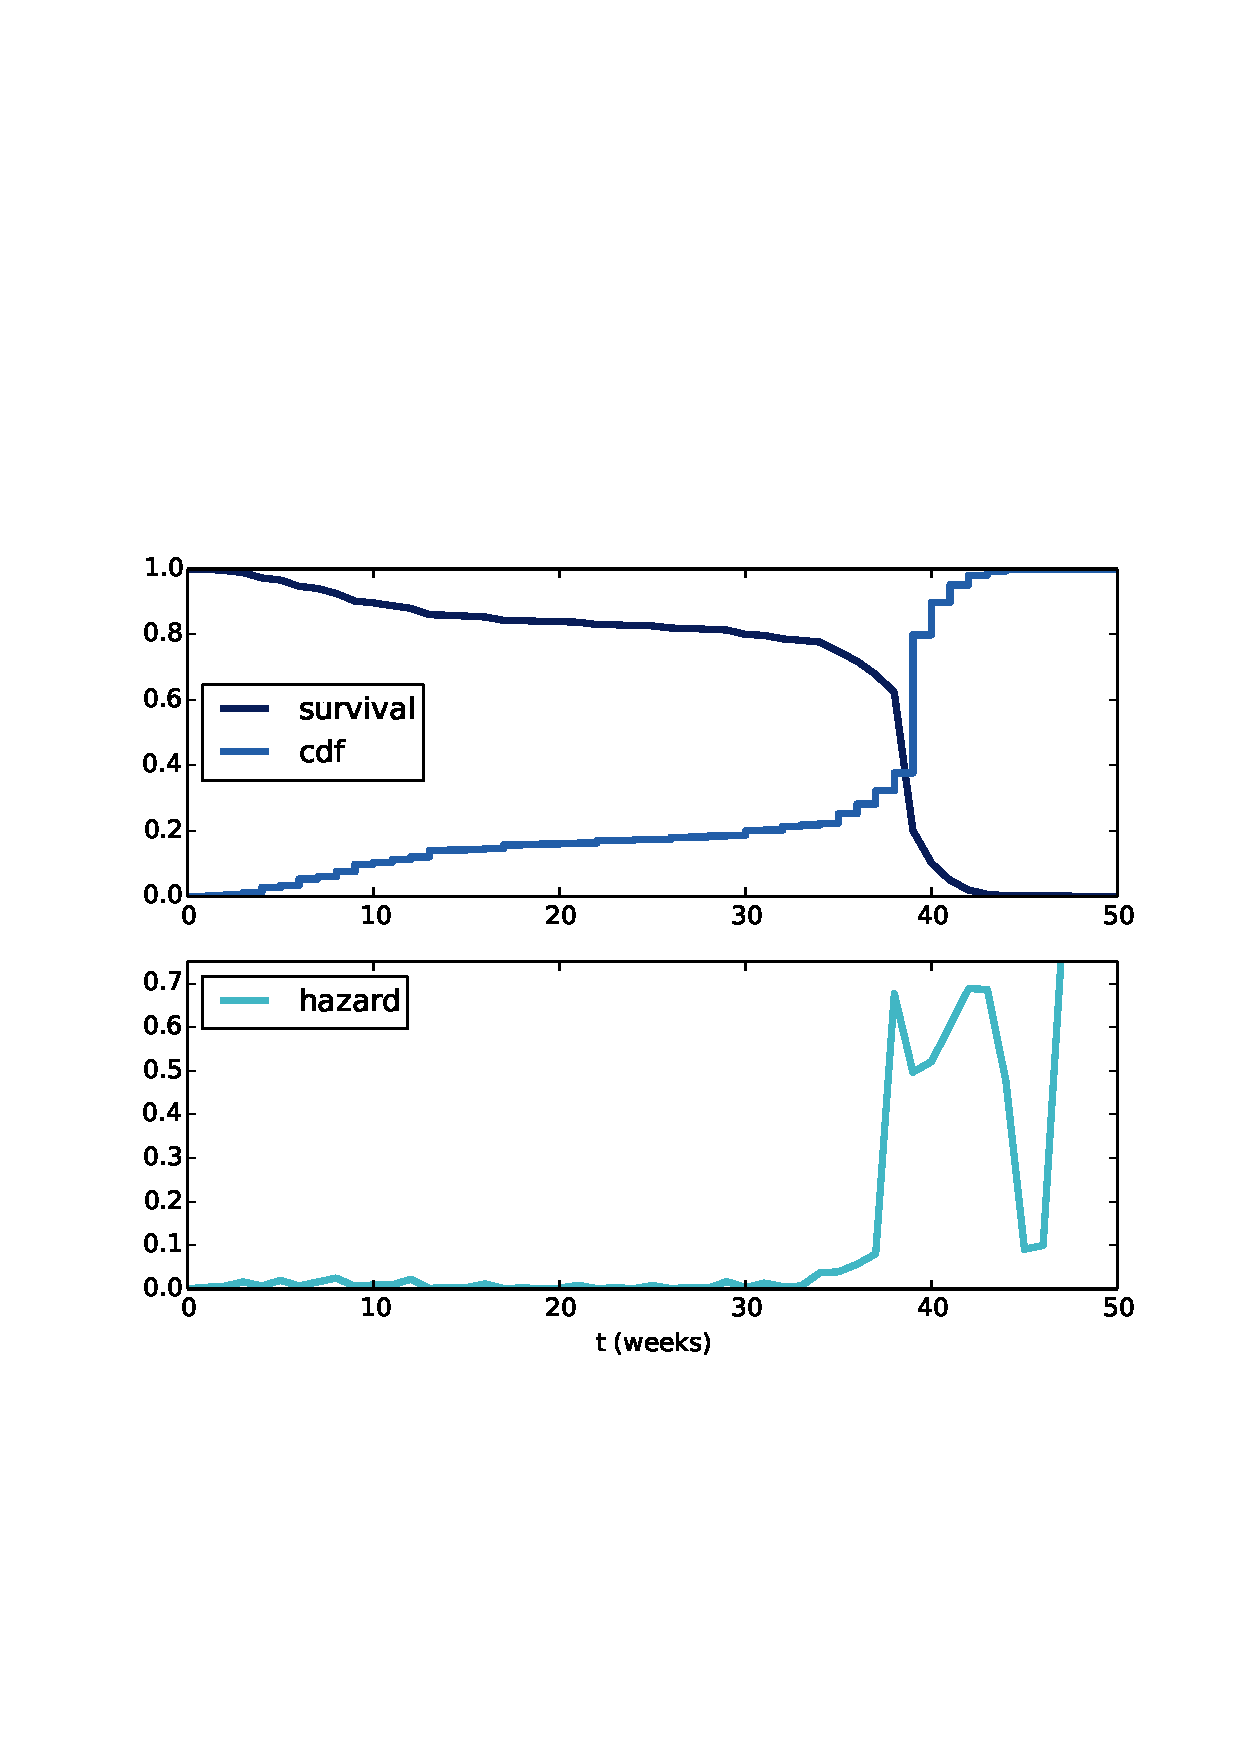
\includegraphics[height=3.0in]{figs/survival1.pdf}}
\caption{임신기간에 대한 CDF와 생존함수(위쪽), 위험함수(아래쪽).}
\label{survival1}
\end{figure}

그림~\ref{survival1} (상단)에 임신기간 CDF와 생존함수인 상보 CDF가 보여진다. 생존함수를 표현하기 위해서, 객체를 정의해서 Cdf를 래핑(wrapping) 인터페이스를 조정하여 맞춘다(adapt).
\index{Cdf}
\index{임신기간 (pregnancy length)}
\index{SurvivalFunction}

\begin{verbatim}
class SurvivalFunction(object):
    def __init__(self, cdf, label=''):
        self.cdf = cdf
        self.label = label or cdf.label

    @property
    def ts(self):
        return self.cdf.xs

    @property
    def ss(self):
        return 1 - self.cdf.ps
\end{verbatim}

{\tt SurvivalFunction}는 프로퍼티(property)를 두개 제공한다; {\tt ts}는 수명 시퀀스고, {\tt ss}는 생존함수다.
파이썬에서 ``프로퍼티(property)''는 마치 변수처럼 호출할 수 있는 메쏘드다.

수명 CDF를 인자로 넘김으로써 {\tt SurvivalFunction}를 인스터스화할 수 있다.
\index{프로퍼티 (property)}

\begin{verbatim}
    sf = SurvivalFunction(cdf)
\end{verbatim}

또한 {\tt SurvivalFunction}는 \verb"__getitem__"와 {\tt Prob}을 제공하는데 생존함수를 평가한다.

\begin{verbatim}
# class SurvivalFunction

    def __getitem__(self, t):
        return self.Prob(t)

    def Prob(self, t):
        return 1 - self.cdf.Prob(t)
\end{verbatim}

예를 들어, {\tt sf[13]} 는 임신초기 3개월을 지난 임신 비율이다.
\index{임신 3개월 (trimester)}

\begin{verbatim}
>>> sf[13]
0.86022
>>> cdf[13]
0.13978
\end{verbatim}

약 86\% 임신이 첫 3개월을 지났다; 약 14\% 그렇지 못하다.

{\tt SurvivalFunction}는 {\tt Render} 기능있다. 그래서,
{\tt thinkplot}에 함수를 사용해서 {\tt sf} 플롯을 그릴 수 있다.
\index{thinkplot}

\begin{verbatim}
    thinkplot.Plot(sf)
\end{verbatim}

그림~\ref{survival1} (상단)에 결과가 나와 있다.

곡선은 거의 13주차에서 26주차는 거의 평평해서, 임신 중기에는 임신 몇몇사례만 중단되는 것을 보여준다. 그리고, 곡선이 39주차에 가장 가파른데 가장 흔한 임신기간이다.
\index{임신기간 (pregnancy length)}


\section{위험 함수 (Hazard function)}
\label{hazard}

생존함수에서 {\bf 위험함수(hazard function)}를 도출할 수 있다; 임신기간에 대해서, 위험함수는 시간 $t$에서 t까지 계속되고 나서 t에서 끝나는 임신 비율이다. 좀더 정확하게는 다음과 같다.

%
\[ \lambda(t) = \frac{S(t) - S(t+1)}{S(t)} \]
%

분자는 $\PMF(t)$로 $t$에서 끝나는 수명 비율이다.
\index{위험함수 (hazard function)}

{\tt SurvivalFunction}는 {\tt MakeHazard} 함수를 제공하는데, 위험 함수를 계산한다.

\begin{verbatim}
# class SurvivalFunction

    def MakeHazard(self, label=''):
        ss = self.ss
        lams = {}
        for i, t in enumerate(self.ts[:-1]):
            hazard = (ss[i] - ss[i+1]) / ss[i]
            lams[t] = hazard

        return HazardFunction(lams, label=label)
\end{verbatim}

{\tt HazardFunction} 객체는 판다스 시리즈 에 대한 랩퍼다. 
\index{판다스 (pandas)}
\index{시리즈 (Series)}
\index{랩퍼 (wrapper)}

\begin{verbatim}
class HazardFunction(object):

    def __init__(self, d, label=''):
        self.series = pandas.Series(d)
        self.label = label
\end{verbatim}

{\tt d}는 딕셔너리 혹은 또다른 시리즈를 포함해서 시리즈를 초기화할 수 있는 다른 어떤 자료형도 될 수 있다. {\tt label}은 플롯으로 그림을 그렸을 때, {\tt HazardFunction}을 식별하는데 사용되는 문자열이다.
\index{HazardFunction}

{\tt HazardFunction}은 \verb"__getitem__"을 제공해서, 다음과 같이 평가할 수 있다.

\begin{verbatim}
>>> hf = sf.MakeHazard()
>>> hf[39]
0.49689
\end{verbatim}

So of all pregnancies that proceed until week 39, about
50\% end in week 39.

그림~\ref{survival1} (아래)에 임신 기간에 대한 위험함수가 보여진다.
임신 42주차 이후 시간에 대해, 위험함수가 불규칙한데, 적은 사례에 기초하기 때문이다. 그 부분을 제외하고, 곡선 모양은 예상한 것과 같다; 약 39주차에 가장 높고, 임신 중기보다 초기에 약간 더 높다.

\index{임신기간 (pregnancy length)}

위험함수는 그자체로 유용하지만, 또한 다음 절에서 살펴보듯이, 생존곡선을 추정하는데 중요한 도구가 된다.

\section{생존곡선 추정하기}

만약 누군가 여러분에게 수명 CDF를 준다면, 생존함수와 위험함수를 계산하기는 쉽다. 하지만, 많은 현실 시나리오에서, 직접 수명분포를 측정할 수는 없다.
유추해야만 한다.
\index{생존곡선 (survival curve)}
\index{CDF}

예를 들어, 진단뒤에 얼마나 오랜기간동안 환자가 생존하는지 살펴보기 위해서 한 환자집단을 추적조사한다고 가정하자.
모든 환자가 동일한 날에 진단받은 것은 아니다. 그래서 시점 아무때나 일부 환자가 다른 환자보다도 더 오래 생존한다. 만약 환자 일부가 죽는다면, 죽은 환자 생존시간을 알게된다. 여전히 살아 있는 환자에 대해서, 생존시간을 알지 못하지만, 생존시간 하한에 대한 정보는 갖게 된다.
\index{진단 (diagnosis)}

만약 모든 환자가 죽을 때까지 기다린다면, 생존곡선을 계산할 수 있다.
하지만, 새로운 처리(treatment)에 대한 효과성을 평가한다면, 그렇게 오래 기다릴 수는 없다. 불완전한 정보 (incomplete information)를 사용해서 생존곡선을 추정할 방법이 필요하다.
\index{불완전 정보 (incomplete information)}

좀더 명량한 예제로, NSFG 데이터를 사용해서 응답자가 초혼 때까지 얼마나 오래 ``생존(survive)''하는지 정량화할 것이다. 
응답자 연령 범위는 14세에서 44세까지다. 그래서, 데이터셋이 일생에서 서로다른 단계에 있는 여성의 스탭샷(snapshot) 정보를 제공한다. 

\index{결혼상태 (marital status)}

결혼한 여성에 대해서, 데이터셋에는 초혼 날짜와 그 당시 연령 정보가 포함되어 있다. 결혼하지 않은 여성에 대해서는 인터뷰했을 당시 연령정보가 있지만, 언제 혹은 결혼을 할 것인지 알 수 있는 방법이 없다.

\index{연령 (age)}

{\em 몇몇} 여성에 대한 초혼 연령을 알고 있기 때문에, 나머지를 제외하고 정보가 있는 데이터 CDF를 계산하고 싶은 유혹이 있다. 이것은 매우 바람직하지 못하다. 결과가 두가지 방향에서 잘못 도출될 수 있다; (1) 좀더 나이가 많은 여성이 더 많이 대표 표본으로 되는데, 인터뷰 당시 좀더 결혼할 것 같기 때문이다. (2) 결혼한 여성이 더 많이 대표 표본이 될 것이다. 사실, 분석 결과 모든 여성은 결혼한다는 결론이 도출될 것이다. 하지만 분명하게 틀렸다.


\section{캐플란-마이어 추정 (Kaplan-Meier estimation)}

이번 예제에서, 결혼하지 않은 여성 관측정보를 포함하는 것은 바람직할 뿐만 아니라 필요한데 이유는 생존분석에서 중심적인 알고리즘 중의 하나인 {\bf 캐플란-마이어 추정(Kaplan-Meier estimation)}과 연결되기 때문이다.
\index{캐플란-마이어 추정 (Kaplan-Meier estimation)}

일반적인 생각은 데이터를 사용해서, 위험함수를 추정하고 나서, 위험함수를 생존함수로 전환한다. 위험함수를 추정하기 위해서, 각 연령별로 다음을 고려한다. (1) 그 연령에 결혼한 여성 숫자, (2) 결혼 ``위험 상태(at risk)''에 있는 여성 숫자로 이전 연령에서 결혼하지 않은 모든 여성이 포함된다.

\index{위험함수 (hazard function)}
\index{위험 상태(at risk)}

다음에 코드가 있다.

\begin{verbatim}
def EstimateHazardFunction(complete, ongoing, label=''):

    n = len(complete)
    hist_complete = thinkstats2.Hist(complete)
    sf_complete = SurvivalFunction(thinkstats2.Cdf(complete))

    m = len(ongoing)
    sf_ongoing = SurvivalFunction(thinkstats2.Cdf(ongoing))

    lams = {}
    for t, ended in sorted(hist_complete.Items()):
        at_risk = ended + n * sf_complete[t] + m * sf_ongoing[t]
        lams[t] = ended / at_risk

    return HazardFunction(lams, label=label)
\end{verbatim}

{\tt complete}는 완벽한 관측 집단이다; 이 경우에 응답자가 결혼했을 때 연령이 된다. {\tt ongoing}은 완벽하지 못한 관측 집단이다; 이 경우에 인터뷰를 했을 때 미혼인 여성 연령이 된다.

먼저, 응답자가 결혼했을 때 연령 Hist인 \verb"hist_complete",
결혼한 여성에 대한 생존함수, \verb"sf_complete", 미혼 여성에 대한 생존함수 \verb"sf_ongoing"를 미리 계산한다.
\index{Hist}
\index{생존함수 (survival function)}

응답자가 결혼했을 때 루프는 연령을 반복한다. 
{\tt t} 각 값에 대해, {\tt t} 연령에서 결혼한 여성 숫자인 {\tt ended}가 있다. 그리고 나서 다음의 합으로 ``위험 상태(at risk)'' 여성 숫자를 계산한다.

\begin{itemize}

\item {\tt ended}, 연령 {\tt t}에서 결혼한 응답자 숫자.

\item \verb"n * sf_complete[t]", 연령 {\tt t} 뒤에 결혼한 응답자 숫자.

\item \verb"m * sf_ongoing[t]", 연령 {\tt t} 후에 인터뷰한 미혼 응답자 숫자, 그러므로 {\tt t} 시점 혹은 이전에 결혼했는지 알려지지 않았다.

\end{itemize}

시점 {\tt t}에 위험함수 추정값은 \verb"at_risk"에 대한 {\tt ended}의 비율이다.

{\tt lams}은 딕셔너리로 $t$에서 $\lambda(t)$으로 매핑한다. 
결과는 {\tt HazardFunction} 객체다.
\index{HazardFunction}


\section{결혼 곡선 (marriage curve)}

이 함수를 검정하기 위해서, 데이터 정제와 변환을 수행해야 한다.
필요한 NSFG 변수는 다음과 같다.

\index{결혼상태 (marital status)}

\begin{itemize}

\item {\tt cmbirth}: 모든 응답자에 대해서 알려진, 응답자 생년월일.
\index{생년월일 (date of birth)}

\item {\tt cmintvw}: 모든 응답자에 대해 알려진, 응답자가 인터뷰한 날짜.

\item {\tt cmmarrhx}: 알려져있고 해당되면, 응답자가 첫 혼인한 날짜.

\item {\tt evrmarry}: 만약 인터뷰 날짜 이전에 결혼했다면 1, 그렇지 않으면 0.

\end{itemize}

첫 변수 세개는 ``세기-월(century-months)'' 방식으로 부호화되었다; 즉, 1899년 12월 이후 정수형 개월 숫자. 그래서, 세기-월(century-month) 1은 1900년 1월이 된다.
\index{세기 월 (century month)}

첫째, 응답자 파일을 읽고, {\tt cmmarrhx}에 있는 타당하지 않는 값 (invalid value)을 교체한다.

\begin{verbatim}
    resp = chap01soln.ReadFemResp()
    resp.cmmarrhx.replace([9997, 9998, 9999], np.nan, inplace=True)
\end{verbatim}

그리고 나서, 혼인 당시에 각 응답자 연령과 인터뷰 당시 연령을 계산한다.
\index{NaN}

\begin{verbatim}
    resp['agemarry'] = (resp.cmmarrhx - resp.cmbirth) / 12.0
    resp['age'] = (resp.cmintvw - resp.cmbirth) / 12.0
\end{verbatim}

다음에, {\tt complete} 변수에 결혼한 여성에 대해서 결혼 당시 연령 정보를 뽑아낸다. 그리고, {\tt ongoing} 변수에 결혼하지 않은 여성에 대한 인터뷰 당시 연령 정보를 대입한다.
\index{연령 (age)}

\begin{verbatim}
    complete = resp[resp.evrmarry==1].agemarry
    ongoing = resp[resp.evrmarry==0].age
\end{verbatim}

마지막으로, 위험함수를 계산한다.
\index{위험함수 (hazard function)}

\begin{verbatim}
    hf = EstimateHazardFunction(complete, ongoing)
\end{verbatim}

그림~\ref{survival2} (위)에 추정 위험함수가 그려져 있다; 10대에는 낮고, 20대에는 더 높고, 30대에는 감소한다. 40대에 다시 증가한다. 하지만, 이것은 추정 과정의 산출물이다; ``위험 상황(at risk)'' 응답자 숫자가 감소함에 따라, 혼인한 적은 여성이 높은 추정 위험을 산출한다. 생존함수는 이러한 잡음을 부드럽게 평활한다.
\index{잡음 (noise)}


\section{생존함수 추정하기}

위험함수를 갖게 되면, 생존함수를 추정할 수 있다.
{\tt t} 시점을 지나 생존할 가망성은 줄곤 살아서 {\tt t} 시점까지 생존할 가망성이 되는데, 보수 위험함수(complementary hazard function)의 누적 곱이 된다.

%
\[ [1-\lambda(0)] [1-\lambda(1)] ... [1-\lambda(t)] \]
%

{\tt HazardFunction} 클래스는 상기 누적곱을 계산하는 {\tt MakeSurvival} 함수를 제공한다.
\index{누적곱 (cumulative product)}
\index{SurvivalFunction}

\begin{verbatim}
# class HazardFunction:

    def MakeSurvival(self):
        ts = self.series.index
        ss = (1 - self.series).cumprod()
        cdf = thinkstats2.Cdf(ts, 1-ss)
        sf = SurvivalFunction(cdf)
        return sf
\end{verbatim}

{\tt ts}는 위험 함수가 추정되는 시점 시퀀스다.
{\tt ss}는 보수 위험함수 누적곱이다. 따라서, 생존함수가 된다.

{\tt SurvivalFunction}가 구현되는 방식 때문에, {\tt ss} 보수를 계산하고, Cdf를 만들고 나서, SurvivalFunction 객체를 인스턴스화 한다.
\index{Cdf}
\index{보수CDF (complementary CDF)}


\begin{figure}
% survival.py
\centerline{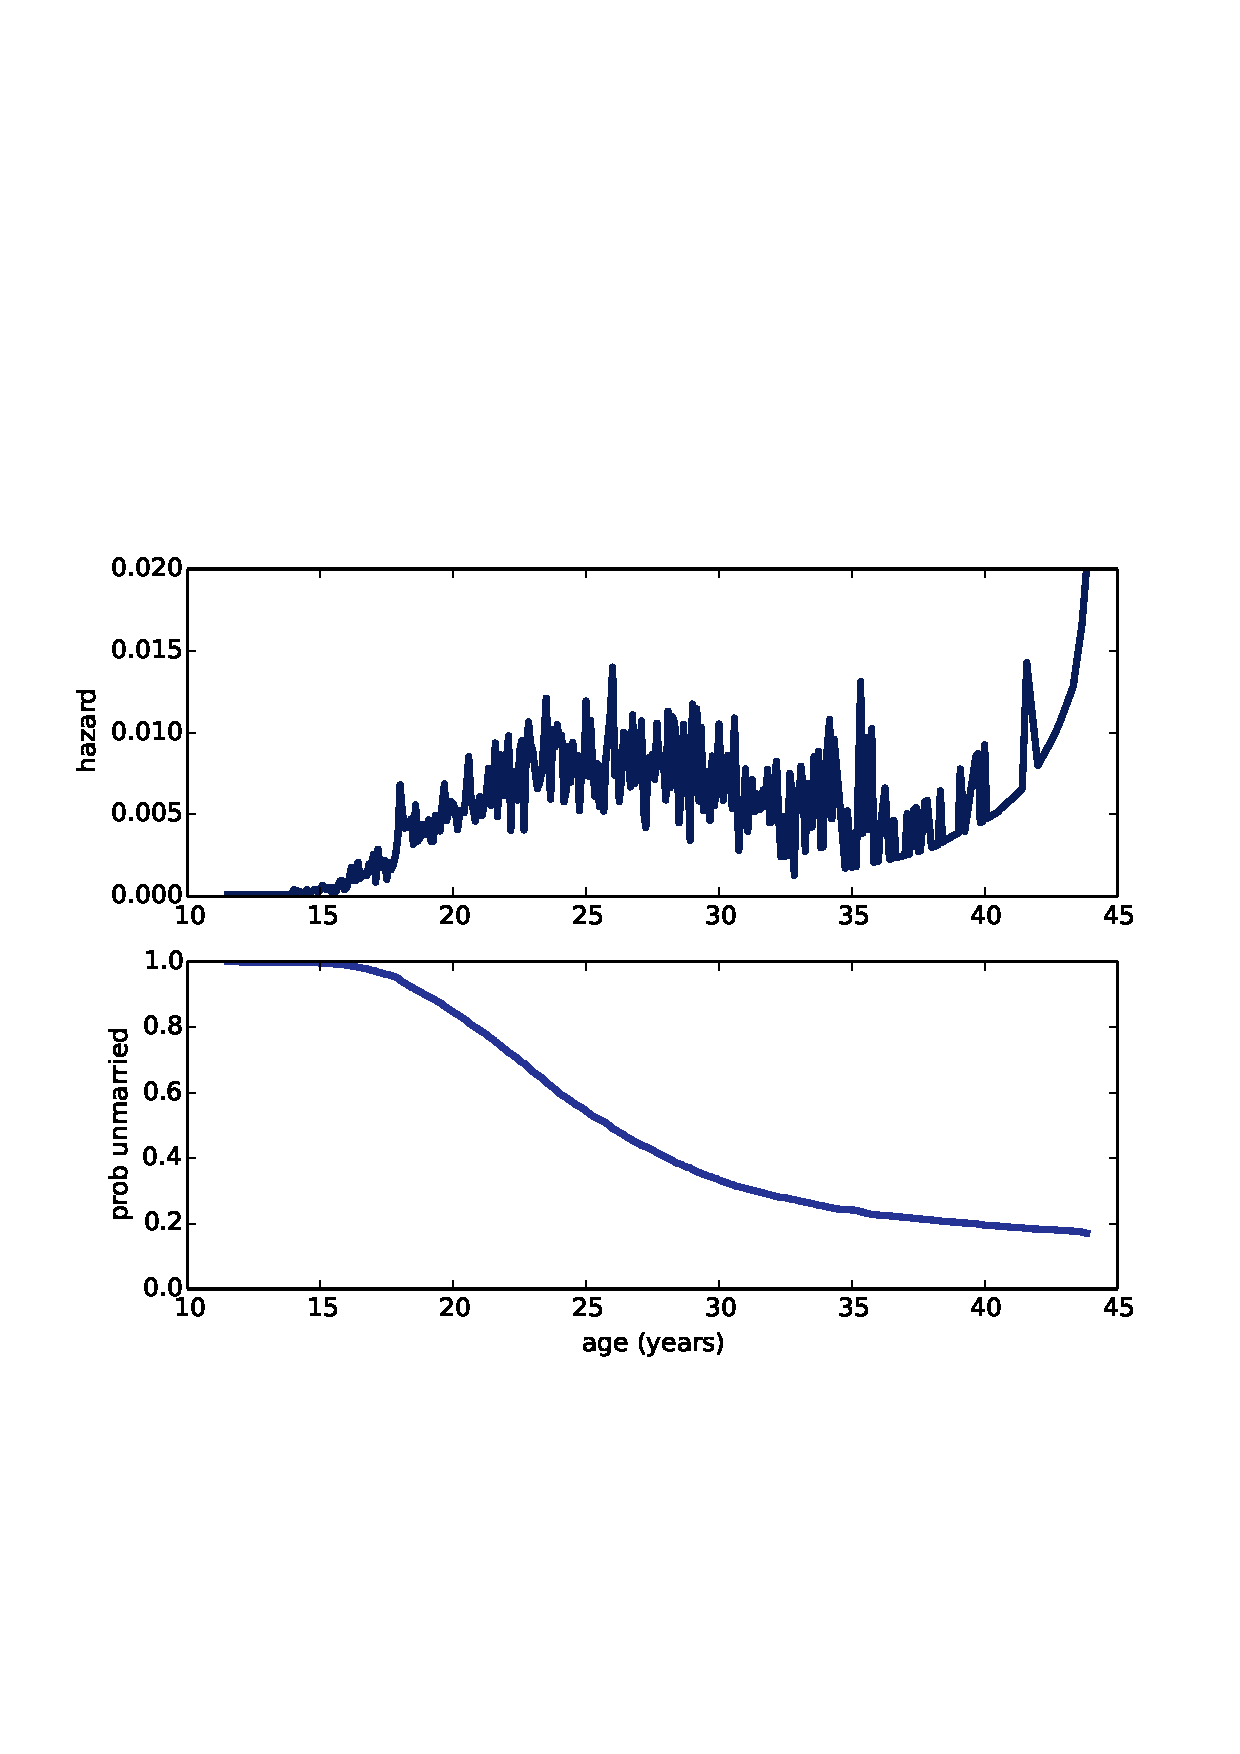
\includegraphics[height=2.5in]{figs/survival2.pdf}}
\caption{초혼 연령에 대한 위험함수(위쪽)와 생존함수(아래쪽).}
\label{survival2}
\end{figure}

그림~\ref{survival2} (아래) 에 결과가 그려져 있다.
생존곡선은 대부분의 여성이 결혼하는 25세에서 35세 사이가 가장 가파르다.
35세에서 45세 사이는 거의 평평하다. 35세 전에 결혼하지 않은 여성이 혼일할 것 같지 않다는 것을 나타낸다.

이와 같은 곡선이 1986년 유명한 잡지기사의 기초가 된다; {\it 뉴스위크(Newsweek)}에 따르면, 40세된 미혼 여성이 혼인보다도 ``테러리스트에 의해 더 살해될 가능성''이 있다. 이러한 통계량은 널리 보도되고 대중적인 문화 일부분이 되었다. 하지만, 그러고 나서 잘못되었다(왜냐하면, 오류가 있는 분석에 기반했기 때문이다) 그리고, 심지어 더 잘못된 것으로 밝혀졌다(이미 진행중이고, 지속되는 문화 변화 때문이다). 2006년 {\it 뉴스위크(Newsweek)}는 보도가 잘못되었다고 시인하는 또다른 기사를 실었다.
\index{뉴스위크 (Newsweek)}

이 기사, 기사의 기반이 된 통계량, 그리고 반응에 관해 더 읽어보기를 격려한다. 신중히 통계분석을 수행하고, 적절한 의심(appropriate skepticism)를 가지고 결과를 해석하고, 공공에게 정확하고 정직하게 제시하는데 있어, 윤리적 책임의 중요성을 상기시켰으면 한다.
\index{윤리 (ethics)}


\section{신뢰구간 (Confidence intervals)}

캐플란-마이어 분석(Kaplan-Meier analysis)은 생존곡선에 대한 단 하나의 추정값을 산출한다. 하지만, 추정값의 불확실성을 정량화하는 것도 또한 중요하다. 늘 그렇듯이, 세가지 오차 원천이 있다; 측정오차, 표집오차, 모형화 오차.

\index{신뢰구간 (confidence interval)}
\index{모형화 오차 (modeling error)}
\index{표집오차 (sampling error)}

이번 예제에서, 측정오차는 대략 작다. 일반적으로, 사람의 출생년월, 혼인여부, 혼인 시점은 알고 있다. 그리고, 이러한 정보를 정확하게 보고할 것으로 예상할 수 있다.
\index{측정 오차 (measurement error)}

재표본추출(resampling)을 통해서 표집오차를 정량화할 수 있다. 다음에 코드가 있다.
\index{재표본추출 (resampling)}

\begin{verbatim}
def ResampleSurvival(resp, iters=101):
    low, high = resp.agemarry.min(), resp.agemarry.max()
    ts = np.arange(low, high, 1/12.0)

    ss_seq = []
    for i in range(iters):
        sample = thinkstats2.ResampleRowsWeighted(resp)
        hf, sf = EstimateSurvival(sample)
        ss_seq.append(sf.Probs(ts))

    low, high = thinkstats2.PercentileRows(ss_seq, [5, 95])
    thinkplot.FillBetween(ts, low, high)
\end{verbatim}

{\tt ResampleSurvival} 함수는 응답자 데이터프레임 {\tt resp}와
재표본추출 횟수 {\tt iters}을 인자로 받는다.
{\tt ts}를 계산하는데 생존함수를 평가하는 연령 시퀀스다.
\index{데이터프레임 (DataFrame)}

루프 내부에, {\tt ResampleSurvival}는 다음과 같다:

\begin{itemize}

\item ~\ref{weighted}절에서 살펴본 {\tt ResampleRowsWeighted}을 사용해서 응답자를 재표본추출한다.
\index{가중 재표본추출 (weighted resampling)}

\item {\tt EstimateSurvival} 호출하는데, 위험곡선과 생존곡선을 추정하는데 앞절 과정을 사용한다.

\item {\tt ts}에 각 연령별로 생존곡선을 평가한다.

\end{itemize}

\verb"ss_seq"는 평가된 생존곡선 시퀀스다. 
{\tt PercentileRows}는 이 시퀀스를 받아 5번째와 95번째 백분위수를 계산하고, 생존곡선 90\% 신뢰구간을 반환한다.
\index{FillBetween}

\begin{figure}
% survival.py
\centerline{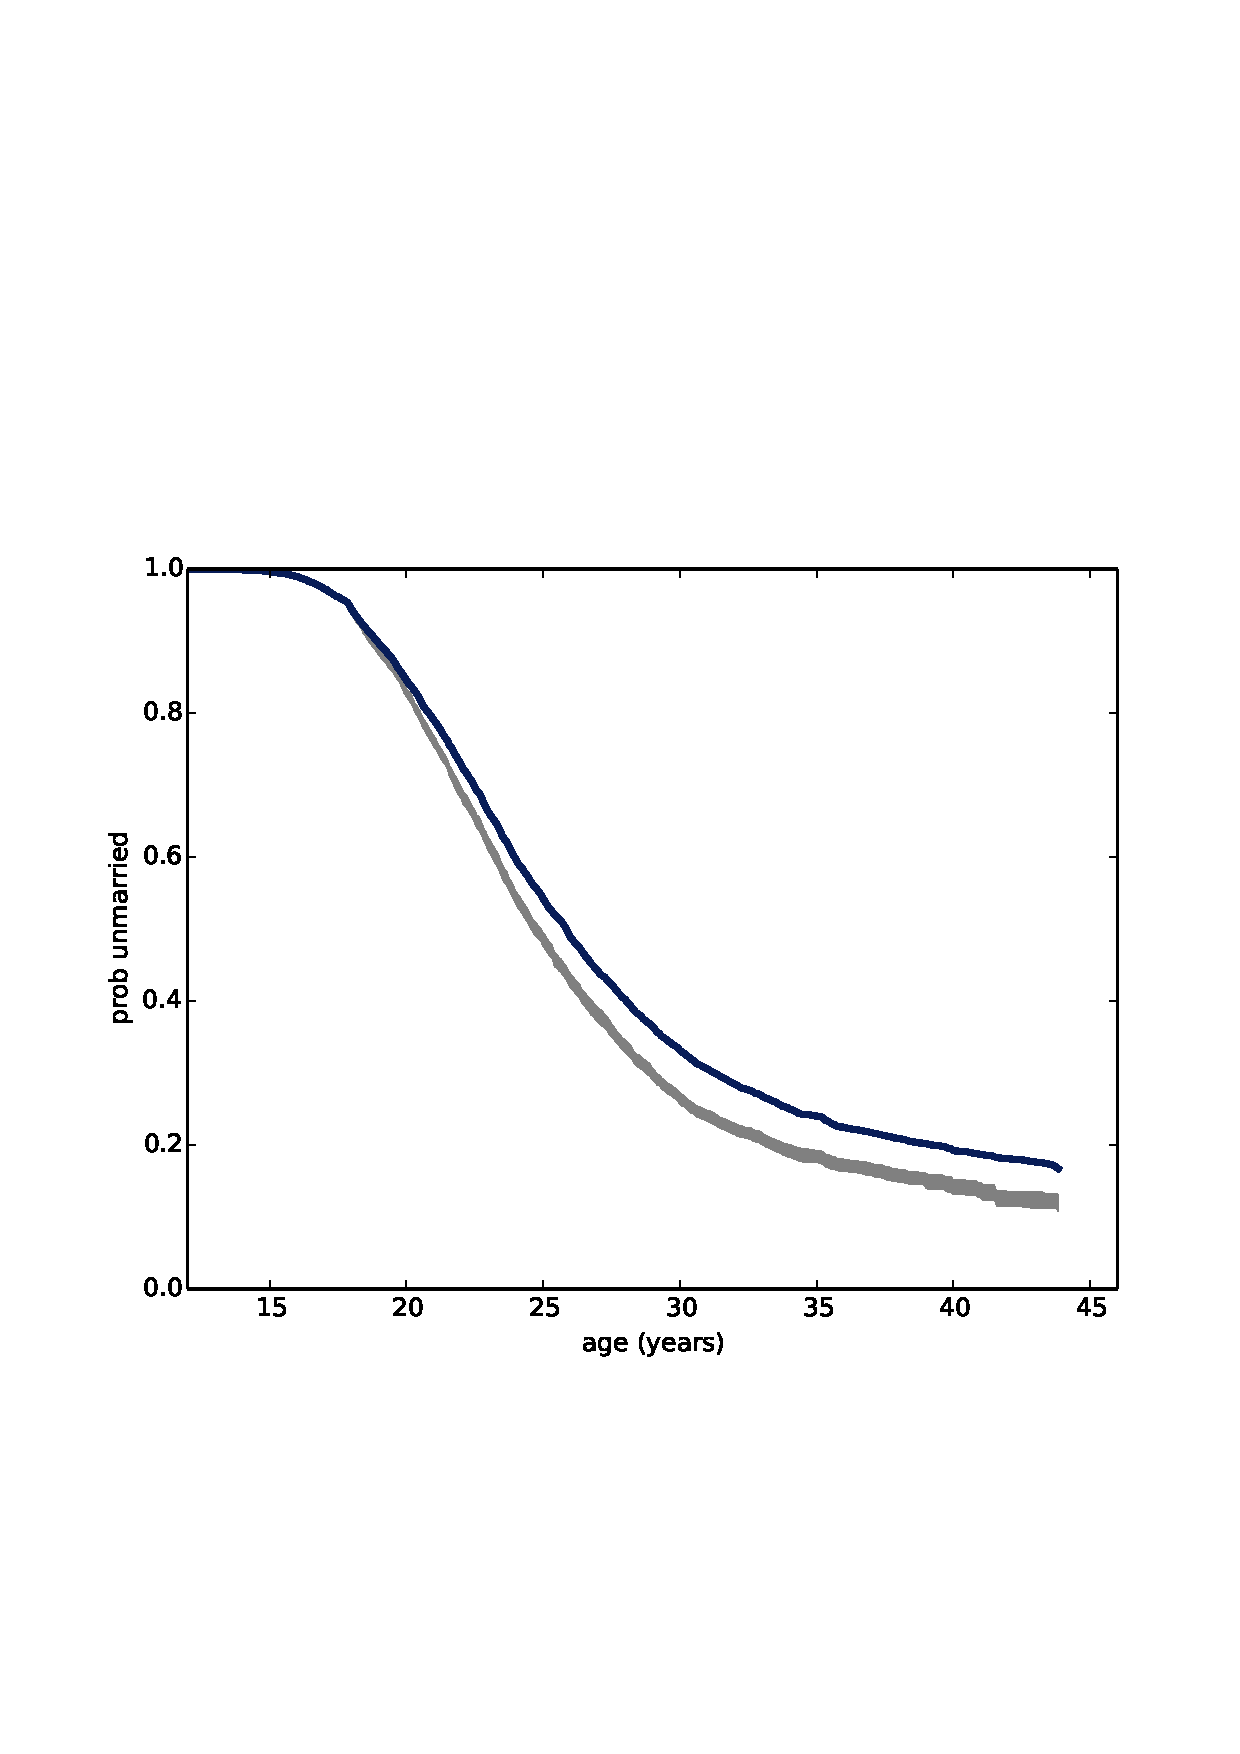
\includegraphics[height=2.5in]{figs/survival3.pdf}}
\caption{초혼연령에 대한 생존함수와 가중 재표집에 근거한 90\% 신뢰구간.}
\label{survival3}
\end{figure}

그림~\ref{survival3}에 앞절에서 추정한 생존함수와 함께 결과가 나와 있다.
신뢰구간은 추정곡선과 달리 표집 가중치(sampling weight)를 고려한다. 둘 사이에 불일치는 표집 가중치가 추정값에 상당한 효과가 있음을 나타낸다---이 사실을 유념해야 한다.
\index{신뢰구간 (confidence interval)}
\index{표집 가중치 (sampling weight)}


\section{코호트 효과 (Cohort effects)}

생존분석 도전중의 하나는 추정 곡선의 다른 부분이 응답자의 다른 집단에 기반한다는 것이다. 시점 {\tt t}에 곡선 부분은 인터뷰 당시에 적어도 응답자 연령이 적어도 {\tt t}인 응답자에 기반한다. 그래서, 곡선의 가장 왼쪽 부분은 모든 응답자로부터 데이터가 포함되어 있고, 가장 오른쪽에는 가장 나이든 응답자만 포함된다.

만약 응답자의 관련 특성이 시간에 따라 변화하지 않는다면, 문제가 되지 않고 좋다. 하지만, 이 경우에  다른 세대에 태어난 여성에 대해서 혼인 패턴은 다를 것 같다. 출생별 10년을 단위로 응답자를 집단화해서 효과를 조사할 수있다.
출생 혹은 비슷한 사건으로 정의되는 이와 같은 집단을 {\bf 코호트(cohorts)}라고 부른다. 그리고, 집단 간 차이를 {\bf 코호트 효과 (cohort effects)}라고 부른다.
\index{코호트 (cohort)}
\index{코호트 효과 (cohort effect)}

NSFG 혼인 데이터에서 코호트 효과를 조사하기 위해서, 이책 전체적으로 사용된 2002년 조사 사이클 6 데이터; ~\ref{replication}절에서 사용된 2006--2010 조사 사이클 6 데이터; 1995년 사이클 5 데이터를 수집했다. 모두 합쳐 데이터셋에는 30,769 응답자가 있다.

\begin{verbatim}
    resp5 = ReadFemResp1995()
    resp6 = ReadFemResp2002()
    resp7 = ReadFemResp2010()
    resps = [resp5, resp6, resp7]
\end{verbatim}

{\tt resp} 각 데이터프레임에 대해서, {\tt cmbirth}를 사용해서 각 응답자에 대한 출생 십년을 계산한다.
\index{판다스 (pandas)}
\index{데이터프레임 (DataFrame)}

\begin{verbatim}
    month0 = pandas.to_datetime('1899-12-15')
    dates = [month0 + pandas.DateOffset(months=cm) 
             for cm in resp.cmbirth]
    resp['decade'] = (pandas.DatetimeIndex(dates).year - 1900) // 10
\end{verbatim}

{\tt cmbirth}은 1899년 12월 이후 정수형 개월수로 부호화된다; {\tt month0}는 Timestamp 객체로 날짜를 표현한다. 각 출생일에 대해 {\tt DateOffset}를 인스턴스화하고, 세기-월을 포함하고 {\tt month0}에 더한다; 결과는 
Timestamps 시퀀스로 {\tt DateTimeIndex}로 전환된다. 마지막으로 {\tt year}를 추출하고 십년단위로 계산한다.
\index{DateTimeIndex}
\index{인덱스 (Index)}
\index{세기 월 (century month)}

표집 가중치를 고려하고, 표집오차 때문에 변동성을 보여주기 위해, 데이터를 재표본추출하고, 십년 단위로 응답자를 집단화하고, 생존곡선을 플롯으로 그린다.
\index{재표본추출 (resampling)}
\index{표집오차 (sampling error)}

\begin{verbatim}
    for i in range(iters):
        samples = [thinkstats2.ResampleRowsWeighted(resp) 
                   for resp in resps]
        sample = pandas.concat(samples, ignore_index=True)
        groups = sample.groupby('decade')

        EstimateSurvivalByDecade(groups, alpha=0.2)
\end{verbatim}

세개 NSFG 시이클 데이터는 서로 다른 표집 가중치를 사용한다. 그래서, 개별적으로 재표본추출하고 나서, {\tt concat}를 사용해서, 하나의 데이터프레임으로 병합한다. 모수 \verb"ignore_index"는 {\tt concat}에게
인덱스로 응답자를 매칭하지 못하게 한다; 대신에 0에서 30768까지 새로운 인덱스를 생성한다.
\index{판다스 (pandas)}
\index{데이터프레임 (DataFrame)}
\index{groupby}

{\tt EstimateSurvivalByDecade}는 각 코호트에 대해서 생존곡선을 플롯으로 그린다.

\begin{verbatim}
def EstimateSurvivalByDecade(resp):
    for name, group in groups:
        hf, sf = EstimateSurvival(group)
        thinkplot.Plot(sf)
\end{verbatim}

\begin{figure}
% survival.py
\centerline{\includegraphics[height=2.5in]{figs/survival4.pdf}}
\caption{서로 다른 십년동안 출생한 응답자에 대한 생존함수.}
\label{survival4}
\end{figure}

그림~\ref{survival4}에 결과가 나와있다.
패턴 몇개가 눈에 보인다.

\begin{itemize}

\item 50년대 여성이 가장 일찍 결혼했고, 연속 코호트 혼인은 점점 늦어지고, 적어도 30대 연령까지 그렇다.

\item 60년에 태어난 여성에는 놀라운 패턴이 있다.
25세 이전에 그전 세대보다 혼인 속도가 더 늦었다. 25세 이후에는 혼인 속도가 더 빠르다. 32세경에는 50년대 코호트를 따라잡고, 44세경에는 상당히 더 결혼상태에 있을 것 같다.
\index{혼인상태 (marital status)}

60년대 태어난 여성은 1985년에서 1995년 사이 25세를 넘어선다.
앞서 언급한 {\it 뉴스위크 (Newsweek)} 기사가 1986년에 보도된 것을 기억하면, 이 기사가 결혼붐에 단초를 제공했다고 상상할 마음이 생긴다. 
이런 설명이 너무 쉬운 것이지만, 기사와 기사에 대응이 이 코호트 행동에 영향을 주었다는 기분을 나타낸다는 것도 가능하다.
\index{뉴스위크 (Newsweek)}

\item 70년대 패턴도 비슷하다. 25세 이전에 혼인하는 것이 그 전세대만 못하다. 하지만, 35세경에 이전 두세대 코호트를 모두 따라잡는다.

\item 80년생 여성은 25세전에 훨씬 덜 혼인할 것 같다. 이후에 일어난 것은 명분명하지 않다; NSFG 다음 사이틀 데이터를 기다려야만 한다.

\end{itemize}

그동안 예측도 할 수 있다.
\index{예측 (prediction)}


\section{외삽법 (Extrapolation)}

70년대생 코호트 생존곡선은 약 38세에서 끝난다; 80년대생 코호트는 약 28세에서 끝나고, 90년대생 코호트는 거의 어떤 자료도 없다.
\index{외삽법 (extrapolation)}

이전 코호트에서 데이터를 ``빌려옴(borrowing)''으로써 이들 곡선을 외삽(extrapolate)할 수 있다. 
HazardFunction에는 {\tt Extend} 메쏘드를 제공하는데, 또다른 더 긴 HazardFunction에서 꼬리를 복사한다.
\index{HazardFunction}

\begin{verbatim}
# class HazardFunction

    def Extend(self, other):
        last = self.series.index[-1]
        more = other.series[other.series.index > last]
        self.series = pandas.concat([self.series, more])
\end{verbatim}

~\ref{hazard}절에서 살펴봤듯이, HazardFunction은 $t$에서 $\lambda(t)$로 매핑하는 시리즈를 담고 있다. {\tt Extend}는 {\tt self.series}에 마지막 인덱스인 {\tt last}를 찾고, {\tt last} 다음에 오는 값을 {\tt other}에서 선택하고, {\tt self.series}에 덧붙인다.
\index{판다스 (pandas)}
\index{시리즈 (Series)}

이제 각 코호트에 대해서 이전 것에서 가져온 값을 사용해서 HazardFunction을 연장할 수 있다.

\begin{verbatim}
def PlotPredictionsByDecade(groups):
    hfs = []
    for name, group in groups:
        hf, sf = EstimateSurvival(group)
        hfs.append(hf)

    thinkplot.PrePlot(len(hfs))
    for i, hf in enumerate(hfs):
        if i > 0:
            hf.Extend(hfs[i-1])
        sf = hf.MakeSurvival()
        thinkplot.Plot(sf)
\end{verbatim}

{\tt groups}는 출생을 십년 단위로 나눈 응답자를 갖는 GroupBy 객체다.
첫번째 루프가 각 집단에 대한 HazardFunction을 계산한다.
\index{groupby}

두번째 루프가 이전 세대로부터 값(이전 집단으로부터 값을 포함할 수 있다)으로 각 HazardFunction를 연장한다.
그리고 나서, 각 HazardFunction을 SurvivalFunction로 전환하고 플롯을 그린다.

\begin{figure}
% survival.py
\centerline{\includegraphics[height=2.5in]{figs/survival5.pdf}}
\caption{서로 다른 십년동안 출생한 응답자에 대한 생존함수와 후세 코호트에 대한 예측.}
\label{survival5}
\end{figure}

그림~\ref{survival5}에 결과가 나와있다; 50년대생 코호트를 제거해서 예측값을 좀더 가시적으로 만들었다. 이 결과가 시사하는 바는, 40세경에 가장 최신 코호트는 60대 코호트에 수렴하는데, 결코 혼인하지 않는 비율은 20\% 보다 적다.
\index{시각화 (visualization)}


\section{기대 잔존 수명}

생존곡선이 주어지면, 현재 연령 함수로 기대잔존수명을 계산할 수 있다.
예를 들어, ~\ref{survival}절에서 임신기간 생존함수가 주어지면 출산까지 예상시간을 계산할 수 있다.
\index{임신기간 (pregnancy length)}

첫단계는 수명 PMF를 추출한다. {\tt SurvivalFunction}가 이를 수행하는 메쏘드를 제공한다.

\begin{verbatim}
# class SurvivalFunction

    def MakePmf(self, filler=None):
        pmf = thinkstats2.Pmf()
        for val, prob in self.cdf.Items():
            pmf.Set(val, prob)

        cutoff = self.cdf.ps[-1]
        if filler is not None:
            pmf[filler] = 1-cutoff

        return pmf
\end{verbatim}

SurvivalFunction는 수명 Cdf를 담고 있다는 것을 기억하라. 루프가 Cdf에서 Pmf로 값과 확률을 복사한다.
\index{Pmf}
\index{Cdf}

{\tt cutoff}는 Cdf에 가장 높은 확률로, 만약 Cdf가 완전하다면 1이고, 그렇지 않다면 1보다 작다. 만약 Cdf가 불완전하다면, 완료하기 위해 제공되는 값 {\tt filler}를 꽂아 넣는다,

임신기간 Cdf는 완전하기 때문에, 아직은 이러한 세부사항까지 걱정할 필요는 없다.
\index{임신기간 (pregnancy length)}

다음 단계는 기대잔존수명을 계산하는데, 여기서 ``기대(expected)''는 평균을 의미한다.
{\tt SurvivalFunction}은 또한 이것을 수행하는 메쏘드를 제공한다.
\index{기대잔존수명 (expected remaining lifetime)}

\begin{verbatim}
# class SurvivalFunction

    def RemainingLifetime(self, filler=None, func=thinkstats2.Pmf.Mean):
        pmf = self.MakePmf(filler=filler)
        d = {}
        for t in sorted(pmf.Values())[:-1]:
            pmf[t] = 0
            pmf.Normalize()
            d[t] = func(pmf) - t

        return pandas.Series(d)
\end{verbatim}

{\tt RemainingLifetime}는 인자로 {\tt MakePmf}에 전달되는 {\tt filler}와, 
잔존수명 분포를 요약하는데 사용되는 함수 {\tt func}을 인자로 받는다.

{\tt pmf}는 SurvivalFunction에서 추출된 수명 Pmf다.
{\tt d}는  현재 연령 {\tt t}에서 기대잔존수명으로 매핑 결과를 담고 있다.
\index{Pmf}

루프가 Pmf에 값을 반복 돌린다. {\tt t} 각 값에 대해, 수명이 {\tt t}를 초과한 것을 둔 상태에서, 수명 조건부분포를 계산한다.
Pmf에서 값을 한번에 하나씩 제거하고, 남은 값을 다시 정규화함으로써 이것을 수행한다.

그리고 나서, {\tt func}를 사용해서, 조건부분포를 요약한다.
상기 예제에서, 기간이 {\tt t}를 초과했을 때 결과는 평균임신기간이 된다.
{\tt t}를 빼서, 평균잔존임신기간을 얻는다.
\index{임신기간 (pregnancy length)}

\begin{figure}
% survival.py
\centerline{\includegraphics[height=2.5in]{figs/survival6.pdf}}
\caption{임신기간에 대한 예상 잔존여명(좌측), 초혼까지 시간(년, 우측).}
\label{survival6}
\end{figure}

그림~\ref{survival6} (왼편)에 현재 지속기간의 함수로 기대잔존임신기간이 나와 있다. 예를 들어, 0주차에는 기대잔존기간이 약 34주가 된다.
이것이 만삭(39주)보다 짧은데 이유는 임신 초기에 임신중절이 평균을 낮추기 때문이다. 
\index{임신기간 (pregnancy length)}

임신초기 기간에 곡선이 천천히 떨어진다. 13주차 뒤에는 기대잔존수명이 25주로 단지 9주만  떨어진다. 그 후에, 곡선은 주마다 약 1주씩 더 빨리 떨어진다. 

37주에서 42주 사이, 곡선은 1주와 2주 사이 수평을 유지한다. 이 기간동안 아무 시점이나 평균잔존기대수명은 같다; 매주 지나감에 따라 목표가 더이상 가까와지지 않는다. 이와 같은 특성을 가진 과정을 {\bf 무기억성(memoryless)}이라고 부른다. 이유는 과거가 예측에 아무런 효과가 없기 때문이다. 
ㅇ 행동이 산부인과 간호사의 격노하는 만트라의 수학적 기반이 된다: ``곧 지금이라도 (any day now)''
\index{무기억성 (memoryless)}

그림 ~\ref{survival6} (오른쪽)에는 연령의 함수로 초혼까지 중위수 잔존시간이 나와있다. 11살 소녀에게 초혼까지 중위수 시간은 약 14년이다. 곡선은 중위수 잔존시간이 약 7년일때 22세까지 감소한다.
그 후에 다시 올라간다: 나이 30에 시작한 연령 14년으로 다시 증가한다.

이 데이터에 기반해서, 젊은 여성은 감소하는 잔존 ``수명''을 갖는다.
이와 같은 성질을 가진 기계부품을 {\bf NBUE}(``new better than used in expectation")로 부른다. 새부품이 더 오래 갈 것으로 예상된다는 의미다.
\index{NBUE}

22세 이상되는 여성은 초혼까지 증가하는 잔존시간을 갖는다.
이와 같은 성질을 갖는 부품을 {\bf UBNE}(``used better than new in expectation'')로 부른다. 즉, 부품이 오래될수록, 더 오래 갈 것으로 예상된다. 신생아와 암환자가 또한 UBNE다; 더 오래 살수록 이들의 기대수명은 증가한다.
\index{UBNE}

이 예제에서 Cdf가 불와전해서, 평균대신에 중위수를 계산했다; 
생존곡선이 약 20\% 응답자가 44세 이전에 결혼하지 않을 것으로 추산한다. 이 여성에 대한 초혼 연령은 알려져있지 않고, 존재하지 않을지도 모른다. 그래서 평균을 계산할 수 없다.

\index{Cdf}
\index{중위수 (median)}

미지값(unknown value)을 무한대를 나타내는 특수값 {\tt np.inf}로 바꿔서 미지값을 처리한다. 이렇게 하면 모든 연령에 대해서 평균이 무한대가 된다.
하지만, 잔존수명 50\% 이상이 유한(연령 30세까지 사실이다)하기만 하면 중위수는 잘 정의된다. 이후에 유의미한 기대잔존수명을 정의하는 것은 어렵다.
\index{inf}

다음에 이들 함수를 계산하고 플롯으로 그리는 코드가 있다.

\begin{verbatim}
    rem_life1 = sf1.RemainingLifetime()
    thinkplot.Plot(rem_life1)

    func = lambda pmf: pmf.Percentile(50)
    rem_life2 = sf2.RemainingLifetime(filler=np.inf, func=func)
    thinkplot.Plot(rem_life2)
\end{verbatim}

{\tt sf1}는 임신 기간에 대한 생존함수다;
이 경우에 {\tt RemainingLifetime}에 초기설정값을 사용할 수 있다.
\index{임신기간 (pregnancy length)}

{\tt sf2}는 초혼 연령에 대한 생존함수다;
{\tt func}는 Pmf를 인자로 받아 중위수(50번째 백분위수)를 계산하는 함수다.
\index{Pmf}


\section{연습문제}

이번 연습문제에 대한 저자 해답은 \verb"chap13soln.py"에 나와있다.

\begin{exercise}

NSFG 주기 6과 7에서, {\tt cmdivorcx} 변수는 응답자의 만약 적용되다면 
년도-월(century-month)로 부호화된 첫 혼인에 대한 이혼 날짜 정보를 담고 있다.
\index{이혼}
\index{혼인상태}

이혼으로 끝나는 결혼기간과 지금까지 지속되는 혼인 기간을 계산하시오.
결혼기간에 대한 위험함수와 생존함수를 추정하시오.

표집 가중치를 고려해서 재표집을 사용하고, 표집오차를 시각화하는데
재표집으로 나온 표본에서 데이터를 도식화하시오.
\index{재표집}

응답자를 10년주기 출생으로 집단화하고, 가능하면 첫번째 혼인 연령으로 
나누는 것을 고려한다.
\index{groupby}

\end{exercise}


\section{용어 사전}

\begin{itemize}

\item 생존분석 (survival analysis): 수명, 좀더 일반적으로 사건이 일어나기까지 시간을 기술하고 예측하는 방법론 집합.
\index{생존분석 (survival analysis)}

\item 생존곡선 (survival curve): 시점 $t$에 $t$를 지나 생존 확률로 매핑하는 함수.
\index{생존곡선 (survival curve)}

\item 위험함수 (hazard function): 시점 $t$ 에 $t$ 시점까지 생존한 사람이 $t$ 시점에 사망한 비율을 매핑하는 함수.
\index{위험함수 (hazard function)}

\item 캐플란-마이어 추정 (Kaplan-Meier estimation): 위험함수와 생존함수를 추정하는 알고리즘.
\index{캐플란-마이어 추정 (Kaplan-Meier estimation)}

\item 코호트 (cohort): 특정 시간 구간에 생년월일 같은 사건으로 정의된 개체 집단.
\index{코호트 (cohort)}

\item 코호트 효과 (cohort effect): 코호트 사이 차이.
\index{코호트 효과 (cohort effect)}

\item NBUE: 기대잔존수명 성질, ``새 것이 예상하기에 오래된 것보다 좋은 것(New better than used in expectation)''
\index{NBUE}

\item UBNE: 기대잔존수명 성질, ``오래된 부품이 예상하기에 새 것보다 좋은 것(Used better than new in expectation)''
\index{UBNE}

\end{itemize}



\chapter{해석적 방법 (Analytic methods)}
\label{analysis}

이책은 모의시험이나 재표본추출같은 수치해석적 방법(computational methods)에 집중했지만, 해결한 문제중 일부는 훨씬더 빠르게 해결할 수 있는 해석적 해(analytic solution)를 가지고 있다.
\index{재표본추출 (resampling)}
\index{해석적 방법 (analytic methods)}
\index{수치해석적 방법 (computational methods)}

이번 장에서 해석적 방법 일부를 제시하고, 어떻게 동작하는지 설명한다. 이장말미에 탐색적 데이터 분석을 위해서 수치해석적 방법과 해석적 방법 통합에 대한 제언을 한다.

이번 장에서 사용되는 코드는 {\tt normal.py}에 있다.
코드를 다운로드하고 작업하는 것에 대한 정보는 ~\ref{code}을 참조한다.


\section{정규분포}
\label{why_normal}
\index{정규분포 (normal distribution)}
\index{분포(distribution)!정규(normal)}
\index{가우스 분포 (Gaussian distribution)}
\index{분포 (distribution)!가우스 (Gaussian)}

동기부여를 위한 사례로, ~\ref{gorilla} 절에 있던 문제를 검토하자.
\index{고릴라 (gorilla)}

\begin{quotation}
\noindent 야생동물 보호구에서 고릴라를 연구하는 과학자가 있다고 가정하자. 고릴라 9마리 체중을 재서, 표본평균 $\xbar=90$ kg와 표본 표준편차 $S=7.5$ kg을 얻었다. 만약 $\xbar$를 모집단 평균으로 추정한다면, 추정값의 표준오차는 얼마나 될까?
\end{quotation}

이 질문에 대답하기 위해서, $\xbar$ 표집 분포가 필요하다. ~\ref{gorilla}절에서, (고릴라 9마리 체중을 재는) 실험을 모의시험함으로써 분포를 근사했고, 각 모의시험 실험에 대해서 $\xbar$를 계산하고, 추정값 분포를 축적했다.
\index{표준오차 (standard error)}
\index{표준편차 (standard deviation)}

결과는 표집분포를 근사했다. 그리고 나서, 표집분포를 사용해서 표준오차와 신뢰구간을 계산했다.
\index{신뢰구간 (confidence interval)}
\index{표집분포 (sampling distribution)}

\begin{enumerate}

\item 표집분포 표준편차는 추정값의 표준오차다; 이 경우 약 2.5 kg이 된다.

\item 5번째와 95번째 백분위수 표집분포 구간이 90\% 신뢰구간이 된다. 만약 실험을 많이 수행한다면, 추정값이 90\% 신뢰구간에 떨어질 것으로 예상한다. 이 경우 90\% CI는 $(86, 94)$ kg이 된다.

\end{enumerate}

이제 해석적으로 동일한 계산을 수행한다. 성인 여성 고릴라 체중이 대략 정규분포한다는 사실을 이용한다.
정규분포는 분석을 용이하게 하는 성질을 두개 갖고 있다; 선형 변환과 덧셈에 ``닫혀(closed)''있다.
이것이 의미하는 바를 설명하기 위해서, 약간의 표기가 필요하다. 
\index{분석 (analysis)}
\index{선형변환 (linear transformation)}
\index{덧셈, 닫혀있다. (addition, closed under)}

어떤 양(quantity)의 분포 $X$가 모수 $\mu$와 $\sigma$을 갖는 정규분포라면, 다음과 같이 표현할 수 있다.
%
\[ X \sim \normal~(\mu, \sigma^{2})\]
%
여기서, 기호 $\sim$ 는 ``분포한다(is distributed)''를 의미하고, 스크립트 문자 $\normal$는 ``정규(normal)''를 나타낸다.

%The other analytic distributions in this chapter are sometimes
%written $\mathrm{Exponential}(\lambda)$, $\mathrm{Pareto}(x_m,
%\alpha)$ and, for lognormal, $\mathrm{Log}-\normal~(\mu,
%\sigma^2)$.
$X$의 선형변환은 $X' = a X + b$와 같은 것으로, 여기서 $a$와 $b$는 실수다.
\index{선형변환 (linear transformation)}
만약, $X'$이 $X$와 같은 모임(족, family)이면, 분포 모임이 선형변환에 닫혀있다. 정규분포는 이 성질을 갖고 있다; 만약 $X \sim \normal~(\mu,
\sigma^2)$이면,
%
\[ X' \sim \normal~(a \mu + b, a^{2} \sigma^2) \tag*{(1)} \]
%
정규분포는 또한 덧셈에도 닫혀있다.
만약 $Z = X + Y$ 이고, $X \sim \normal~(\mu_{X}, \sigma_{X}^{2})$, $Y \sim \normal~(\mu_{Y}, \sigma_{Y}^{2})$이면,
%
\[ Z \sim \normal~(\mu_X + \mu_Y, \sigma_X^2 + \sigma_Y^2)  \tag*{(2)}\]
%
특별한 경우 $Z = X + X$이면, 다음을 만족한다.
%
\[ Z \sim \normal~(2 \mu_X, 2 \sigma_X^2) \]
%
그리고, 일반적으로 $X$에서 $n$개 값을 추출한다면, 다음을 갖게 된다.
%
\[ Z \sim \normal~(n \mu_X, n \sigma_X^2)  \tag*{(3)}\]


\section{표집분포}

이제 $\xbar$ 표집분포를 계산하는데 필요한 모든 것을 갖췄다. $\xbar$를 계산하는데 $n$개 고릴라 체중을 재고, 더해서 전체 체중값을 얻고 나서, $n$으로 나눈다는 것을 기억하라.
\index{표집분포 (sampling distribution)}
\index{고릴라 (gorilla)}
\index{체중 (weight)}

고릴라 체중 $X$ 분포가 근사적으로 정규분포라고 가정한다.
%
\[ X \sim \normal~(\mu, \sigma^2)\]
%
만약 $n$개 고릴라 체중을 잰다면, 전체체중 $Y$는 3번 방정식을 사용해서 다음과 같이 분포한다.
%
\[ Y \sim \normal~(n \mu, n \sigma^2) \]
%

그리고 만약 $n$으로 나눈다면, $a = 1/n$으로 1번 방정식을 사용해서 표본평균 $Z$는 다음과 같이 분포한다.
%
\[ Z \sim \normal~(\mu, \sigma^2/n) \]
%

$Z$ 분포는 $\xbar$의 표집분포가 된다.
$Z$ 평균은 $\mu$으로, $\xbar$가 $\mu$의 불편 추정값이 된다는 것을 보여준다.
표집분포 분산은 $\sigma^2 / n$이다.
\index{편의 추정량 (biased estimator)}
\index{추정량 (estimator)!편의 (biased)}

그래서, 표집분포 표준편차, 즉 추정값의 표준오차는 $\sigma / \sqrt{n}$이 된다. 예제에서, $\sigma$는 7.5 kg 이고, $n$은 9가 되서, 표준오차는 2.5 kg가 된다.
결과는 모의시험으로 추정한 것과 일치하지만, 계산하기는 훨씬 더 빠르다!
\index{표준오차 (standard error)}
\index{표준편차 (standard deviation)}

또한, 표집분포를 사용해서 신뢰구간도 계산할 수 있다.
$\xbar$에 대한 90\% 신뢰구간은 $Z$의 5번째와 95번째 백분위수 간격이다.
$Z$이 정규분포를 따르기 때문에, 역 CDF(inverse CDF)를 평가해서 백분위수를 계산할 수 있다.
\index{역 CDF (inverse CDF)}
\index{CDF, 역 (CDF, inverse)}
\index{신뢰구간 (confidence interval)}

정규분포 CDF와 역 CDF에 대한 닫힌 형태(closed form)가 존재하지 않지만, 
빠른 수치해석 방법이 존재하고 ~\ref{normal}절에서 살펴본 바와 같이 SciPy에 
구현되어 있다. {\tt thinkstats2}에 SciPy 함수를 좀더 쉽게 사용할 수 있게 하는 랩퍼(wrapper) 함수가 제공된다.
\index{SciPy}
\index{정규분포 (normal distribution)}
\index{랩퍼 (wrapper)}
\index{닫힌 형태 (closed form)}

\begin{verbatim}
def EvalNormalCdfInverse(p, mu=0, sigma=1):
    return scipy.stats.norm.ppf(p, loc=mu, scale=sigma)
\end{verbatim}

확률 {\tt p}가 주어졌을 대, 모수 {\tt mu}와 {\tt sigma}를 갖는 정규분포에서 대응되는 백분위수를 반환한다. 
$\xbar$의 90\% 신뢰구간에 대해서, 
다음과 같이 5번째와 95번째 백분위수를 계산한다.
\index{백분위수 (percentile)}

\begin{verbatim}
>>> thinkstats2.EvalNormalCdfInverse(0.05, mu=90, sigma=2.5)
85.888

>>> thinkstats2.EvalNormalCdfInverse(0.95, mu=90, sigma=2.5)
94.112
\end{verbatim}

그래서, 만약 실험을 많이 반복한다면, 추정값 $\xbar$가 약 90\%로 범위 $(85.9, 94.1)$에 떨어질 것이다. 
다시 이값은 모의시험으로 얻은 결과와 일치한다.
\index{simulation}


\section{정규분포 표현하기}

상기 계산을 좀더 쉽게하기 위해서, {\tt Normal} 클래스를 정의하는데 정규분포를 표현하고 앞절 방정식을 부호화한다. 다음에 코드가 있다.
\index{Normal}

\begin{verbatim}
class Normal(object):

    def __init__(self, mu, sigma2):
        self.mu = mu
        self.sigma2 = sigma2

    def __str__(self):
        return 'N(%g, %g)' % (self.mu, self.sigma2)
\end{verbatim}

그래서, 고릴라 체중 분포를 표현하는 Normal을 인스턴스화할 수 있다.
\index{고릴라 (gorilla)}

\begin{verbatim}
>>> dist = Normal(90, 7.5**2)
>>> dist
N(90, 56.25)
\end{verbatim}

{\tt Normal} 클래스에는 {\tt Sum} 메쏘드가 제공되는데, 표본크기 {\tt n}을 인다로 받아, 방정식 3을 사용해서 {\tt n}개 값의 합계 분포를 반환한다.

\begin{verbatim}
    def Sum(self, n):
        return Normal(n * self.mu, n * self.sigma2)
\end{verbatim}

Normal은 또한 방정식 1을 사용해서 곱셈과 나눗셈도 수행한다.

\begin{verbatim}
    def __mul__(self, factor):
        return Normal(factor * self.mu, factor**2 * self.sigma2)

    def __div__(self, divisor):
        return 1 / divisor * self
\end{verbatim}

그래서, 표본크기 9를 가지고 평균의 표집분포를 계산할 수 있다.
\index{표집분포 (sampling distribution)}
\index{표본크기 (sample size)}

\begin{verbatim}
>>> dist_xbar = dist.Sum(9) / 9
>>> dist_xbar.sigma
2.5
\end{verbatim}

으로 앞절에서 살펴보았듯이, 표집분포 표준편차는 2.5 kg이다.
마지막으로, Normal 클래스에는 {\tt Percentile} 메쏘드가 있어서 신뢰구간을 계산하는데 사용할 수 있다.
\index{표준편차 (standard deviation)}
\index{신뢰구간 (confidence interval)}

\begin{verbatim}
>>> dist_xbar.Percentile(5), dist_xbar.Percentile(95)
85.888 94.113
\end{verbatim}

그리고, 이것은 앞에서 얻은 답과 같다. 나중에 Normal 클래스를 다시 사용할 것이다. 하지만, 더 진도를 나가기 전에, 분석 한가지가 더 필요하다.


\section{중심극한정리 (Central limit theorem)}
\label{CLT}

앞절에서 살펴봤듯이, 만약 정규분포에서 추출한 값을 더하면, 합 분포도 정규분포다. 다른 대부분의 분포는 이런 성질을 갖지 못하다; 만약 다른 분포에서 추출한 값을 더한다면, 합은 일반적으로 해석적 분포를 갖지 못한다.
\index{합(sum)}
\index{정규분포 (normal distribution)} \index{분포 (distribution)!정규 (normal)}
\index{가우스 분포 (Gaussian distribution)} \index{분포 (distribution)!가우스 (Gaussian)}

하지만, 거의 모든 분포에서 {\tt n} 값을 더하면, 합 분포가 {\tt n}이 증가함에 따라 정규분포로 수렴한다.

좀더 구체적으로, 만약 값들의 분포가 평균과 표준편차 $\mu$와 $\sigma$를 갖는다면, 합 분포는 근사적으로 $\normal(n \mu, n \sigma^2)$이 된다.
\index{표준편차 (standard deviation)}

이 결과가 중심극한정리(Central Limit Theorem, CLT)이다.  
통계분석을 위한 가장 유용한 도구 중 하나다. 하지만, 몇가지 주의점이 있다.
\index{중심극한정리 (Central Limit Theorem)}
\index{CLT}

\begin{itemize}

\item 값들이 독립적으로 추출되어야 한다. 만약 상관된다면, CLT을 적용할 수 없다.(설사 이것이 실무에서 문제가 결코되지는 않을지만)
\index{독립적 (independent)}

\item 값들이 동일한 분포에서 나와야 한다 (설사 이런 요구사항은 완화될 수도 있지만)
\index{동일한 (identical)}

\item 유한 평균과 분산을 갖는 분포에서 값들이 나와야 한다. 그래서 대부분 파레토 분포는 해당되지 않는다.
\index{평균 (mean)}
\index{분산 (variance)}
\index{파레토 분포 (Pareto distribution)}
\index{분포 (distribution)!파레토 (Pareto)}
\index{지수분포 (exponential distribution)}
\index{분포 (distribution)!지수 (exponential)}

\item 수렴 속도는 분포 왜도에 의존한다. 지수분포에서 나온 값들의 합은 작은 {\tt n}에 대해서 수렴한다. 로그 정규분포에서 나온 값들의 합은 더 커다란 크기가 필요하다.
\index{로그정규분포 (lognormal distribution)}
\index{분포 (distribution)!로그정규 (lognormal)}
\index{왜도 (skewness)}

\end{itemize}

중심극한정리는 자연 세계에 정규분포가 널리 퍼짐을 설명한다.
생물체의 많은 특징이 유전적 환경적 요인에 영향을 받는데, 이들 효과는 가법(additive)적이다. 측정하는 특징은 많은 작은 효과의 합이다. 그래서, 분포가 정규분포화 되는 경향이 있다.

\index{정규분포 (normal distribution)}
\index{분포 (distribution)!정규 (normal)}
\index{가우스 분포 (Gaussian distribution)}
\index{분포 (distribution)!가우스 (Gaussian)}
\index{중심극한정리 (Central Limit Theorem)}
\index{CLT}


\section{CLT 검정}

중심극한정리가 어떻게 동작하는지와 언제 동작하지 않는지를 살펴보기 위새허, 실험을 몇가지 시도해보자. 먼저, 지수분포로 시도해보자.

\begin{verbatim}
def MakeExpoSamples(beta=2.0, iters=1000):
    samples = []
    for n in [1, 10, 100]:
        sample = [np.sum(np.random.exponential(beta, n))
                  for _ in range(iters)]
        samples.append((n, sample))
    return samples
\end{verbatim}


{\tt MakeExpoSamples}는 지수분포값 합을 생성한다(``지수분포로부터 추출된 값들''을 줄여 ``지수분포값''을 사용한다).
{\tt beta}는 분포 모수다; {\tt iters}는 생성할 합 갯수다.

상기 함수를 설명하기 위해서, 내부에서 시작해서 밖으로 나가면서 마무리한다.
{\tt np.random.exponential}을 매번 호출할 때마다, {\tt n}개 지수분포값 시퀀스를 얻어서 합을 계산한다. {\tt sample}은 길이 {\tt iters}를 갖는 합계 리스트가 된다.
\index{넘파이 (NumPy)}

{\tt n}과 {\tt iters}를 혼동하기 쉽다: {\tt n}은 각 합에 대한 항의 갯수다; {\tt iters}는 합분포를 특성화하기 위해서 계산하는 합 갯수다.

반환되는 값은 {\tt (n, sample)} 쌍(pair) 리스트다. 각 쌍에 대해 정규확률그림을 만들 수 있다.
\index{thinkplot}
\index{정규확률그림 (normal probability plot)}

\begin{verbatim}
def NormalPlotSamples(samples, plot=1, ylabel=''):
    for n, sample in samples:
        thinkplot.SubPlot(plot)
        thinkstats2.NormalProbabilityPlot(sample)

        thinkplot.Config(title='n=%d' % n, ylabel=ylabel)
        plot += 1
\end{verbatim}

{\tt NormalPlotSamples}은 {\tt MakeExpoSamples}에서 리스트 짝(pair)를 인자로 받아 정규확률그림 행을 생성한다.
\index{정규확률그림 (normal probability plot)}

\begin{figure}
% normal.py
\centerline{\includegraphics[height=3.5in]{figs/normal1.pdf}}
\caption{지수분포값의 합에 대한 분포(윗줄), 로그정규분포값의 합에 대한 분포(아랫줄).}
\label{normal1}
\end{figure}

그림~\ref{normal1} (위쪽 행)에 결과가 나와있다.
{\tt n=1}일 때, 합분포는 여전히 지수분포라서 정규확률그림은 직선이 아니다.
하지만, {\tt n=10}일 때, 합분포는 근사 정규분포가 되고,
{\tt n=100}일 때, 정규분포와 거의 구별되지 않는다.

그림~\ref{normal1} (아래 행)에 로그정규분포에 대한 비슷한 결과가 나와 있다.
로그정규분포는 일반적으로 지수분포보다 기울어짐이 더 심해서, 합분포는 수렴하는데 더 오래 걸린다. {\tt n=10}일 때, 정규확률그림은 거의 직선인 곳이 없다. 하지만, {\tt n=100}일 때, 근사적으로 정규분포다.
\index{로그정규 분포 (lognormal distribution)}
\index{분포 (distribution)!로그정규 (lognormal)}
\index{왜도 (skewness)}

\begin{figure}
% normal.py
\centerline{\includegraphics[height=3.5in]{figs/normal2.pdf}}
\caption{
파레토분포값의 합에 대한 분포(윗줄), 상관된 지수분포값의 합에 대한 분포(아랫줄).}
\label{normal2}
\end{figure}

파레토 분포는 로그정규분포보다 더 기울어짐이 심하다. 모수에 따라서, 많은 파레토 분포는 유한 평균과 분산을 갖지 못하다. 결과로, 중심극한정리가 적용되지 않는다. 그림~\ref{normal2} (상단 행)에 파레토 값들의 합 분포가 나와 있다. 심지어 {\tt n=100}일 때, 정규확률그림은 직선에서 거리가 멀다.
\index{파레토 분포 (Pareto distribution)}
\index{분포 (distribution)!파레토 (Pareto)}
\index{중심극한정리 (Central Limit Theorem)}
\index{CLT}
\index{정규확률그림 (normal probability plot)}

또한 CLT는 만약 값들이 상관된다면 적용되지 않는다고 언급했다. 이것을 검정하기 위해서, 지수분포에서 상관된 값들을 생성했다. 
상관된 값을 재생하는데 사용된 알고리즘은 (1) 상관된 정규분포 값을 발생시킨다. (2) 정규분포 CDF를 사용해서 값을 균등분포로 변환한다. (3) 역 지수분포 CDF를 사용해서 균등분포 값을 지수분포로 변환한다.

\index{역 CDF (inverse CDF)}
\index{CDF 역 (CDF, inverse)}
\index{상관 (correlation)}
\index{난수 (random number)}

{\tt GenerateCorrelated}는 계열상관 {\tt rho}를 갖는 {\tt n}개 정규분포 값 반복자를 반환한다.
\index{반복자 (iterator)}

\begin{verbatim}
def GenerateCorrelated(rho, n):
    x = random.gauss(0, 1)
    yield x

    sigma = math.sqrt(1 - rho**2)
    for _ in range(n-1):
        x = random.gauss(x*rho, sigma)
        yield x
\end{verbatim}

첫값은 표준정규분포 값이다. 각 후속값은 이전 값에 의존한다: 만약 이전 값이 {\tt x}, 다음값은 평균 {\tt x*rho}, 분산 {\tt 1-rho**2}이다. 
{\tt random.gauss}는 두번째 인자로 분산이 아닌 표준편차를 받는 것을 주목한다.
\index{표준편차 (standard deviation)}
\index{표준정규분포 (standard normal distribution)}

{\tt GenerateExpoCorrelated}는 결과 시퀀스를 인자로 받아 지수분포 값으로 변환한다.

\begin{verbatim}
def GenerateExpoCorrelated(rho, n):
    normal = list(GenerateCorrelated(rho, n))
    uniform = scipy.stats.norm.cdf(normal)
    expo = scipy.stats.expon.ppf(uniform)
    return expo
\end{verbatim}

{\tt normal}은 상관된 정규분포 값 리스트다.
{\tt uniform}은 0과 1사이 균등분포 값 시퀀스다.
{\tt expo}는 상관된 지수분포 값 시퀀스다.
{\tt ppf}는 ``퍼센트점 함수 (percent point function)''의 약어로 역CDF에 대한 또다른 이름이다.

\index{역CDF (inverse CDF)}
\index{CDF 역 (CDF, inverse)}
\index{퍼센트점 함수 (percent point function)}

그림~\ref{normal2} (하단 행)에 {\tt rho=0.9} 상관을 갖는 지수분포 값 합의 분포가 나와 있다. 상관된 경우 수렴속도가 느리다; 그럼에도 불구, {\tt n=100}일 때, 정규확률그림은 거의 직선이다. 그래서 값들이 상관되었을 때, CLT가 엄격하게 적용되지는 않지만, 적당한 상관은 실무에서 결코 문제가 되지 않는다.
\index{정규확률그림 (normal probability plot)}
\index{상관 (correlation)}

중심극한정리가 어떻게 동작하는지와 중심극한정리가 동작하지 않을 때 무슨일이 발생하는지 보여주기 위해서 이들 실험이 고안되었다. 이제 중심극한정리를 어떻게 사용하는지 살펴보자.


\section{CLT 적용하기}
\label{usingCLT}

왜 중심극한정리가 유용한지 살펴보기 위해서, ~\ref{testdiff}절에 예제로 돌아가자: 첫째아이와 첫째가 아닌 아이에 대한 평균 임신기간 외관효과 검정.
앞에서 살펴봤듯이, 외관 차이는 약 0.078주다.
\index{임신기간 (pregnancy length)}
\index{중심극한정리 (Central Limit Theorem)}
\index{CLT}

\begin{verbatim}
>>> live, firsts, others = first.MakeFrames()
>>> delta = firsts.prglngth.mean() - others.prglngth.mean()
0.078
\end{verbatim}

가설검정 로직을 기억하라: p-값을 계산하는데, 귀무가설 아래에서 관측 차이 확률이다; 만약 작다면, 관측 차이는 우연에 의한 것이 아닐 것으로 결론낸다.
\index{p-값 (p-value0}
\index{귀무가설 (null hypothesis)}
\index{가설검정 (hypothesis testing)}

이 예제애서, 귀무가설은 임신기간 분포가 첫째 아이와 첫째가 아닌 아이들에 대해서 같다. 그래서, 다음과 같이 평균 표집분포를 계산할 수 있다.
\index{표집분포 (sampling distribution)}

\begin{verbatim}
    dist1 = SamplingDistMean(live.prglngth, len(firsts))
    dist2 = SamplingDistMean(live.prglngth, len(others))
\end{verbatim}

두 표집분포는 동일 모집단에 기반하는데 모든 정상 출산을 합동(pool)한 것이다. {\tt SamplingDistMean}는 이 값 시퀀스와 표본크기를 인자로 받아 표집분포를 표현하는 Normal 객체를 반환한다.

\begin{verbatim}
def SamplingDistMean(data, n):
    mean, var = data.mean(), data.var()
    dist = Normal(mean, var)
    return dist.Sum(n) / n
\end{verbatim}

{\tt mean}와 {\tt var}는 {\tt data} 평균과 분산이다.
정규분포 {\tt dist}로 데이터 분포를 근사한다.

이 예제애서 데이터는 정규분포되어 있지 않다. 그래서 이러한 근사가 그다지 좋지 않다. 하지만 그리고 나서 {\tt dist.Sum(n) / n}을 계산하는데 {\tt n}개 값 평균의 표집분포다. 데이터가 정규분포되어 있지 않지만, 평균 표집분포는 중심극한정리에 의해서 정규분포된다.
\index{중심극한정리 (Central Limit Theorem)}
\index{CLT}

다음, 평균에 차이 표집분포를 계산한다.
{\tt Normal} 클래스는 방정식 2를 사용해서 뺄셈을 어떻게 수행하는지 알고 있다.
\index{Normal}

\begin{verbatim}
    def __sub__(self, other):
        return Normal(self.mu - other.mu,
                      self.sigma2 + other.sigma2)
\end{verbatim}

그래서, 다음과 같이 차이 표집분포를 계산할 수 있다.

\begin{verbatim}
>>> dist = dist1 - dist2
N(0, 0.0032)
\end{verbatim}

평균은 0 인데, 일리가 있다. 왜냐하면 평균적으로 동일 분포에서 추출된 두 표본은 같은 평균을 갖을 것으로 예상하기 때문이다. 표집분포 분산은 0.0032가 된다.
\index{표집분포 (sampling distribution)}

{\tt Normal} 클래스는 {\tt Prob}메쏘드를 제공하는데 정규분포 CDF를 평가한다. {\tt Prob}를 사용해서 귀무가설 아래에서 차이 확률을 {\tt delta} 만큼 계산할 수 있다.
\index{귀무가설 (null hypothesis)}

\begin{verbatim}
>>> 1 - dist.Prob(delta)
0.084
\end{verbatim}

의미하는 바는 단측검정에 대한 p-값이 0.084다. 양측검정에 대해서 또한 다음과 같이 계산한다.
\index{p-값 (p-value)}
\index{단측검정 (one-sided test)}
\index{양측검정 (two-sided test)}

\begin{verbatim}
>>> dist.Prob(-delta)
0.084
\end{verbatim}

정규분포는 대칭이기 때문에 동일하다. 꼬리 합은 0.168로, ~\ref{testdiff}절 추정값과 일치한다; 값이 0.17이였다.
\index{대칭(symmetric)}



\section{상관검정 (Correlation test)}

~\ref{corrtest}절에서 출생 체중과 산모 연령 사이 상관을 계산하는데 순열검정(permutation test)을 사용했고, p-값이 0.001보다 작아 통계적으로 유의적이라는 것을 발견했다.
\index{p-값 (p-value)}
\index{출생체중 (birth weight)}
\index{체중 (weight)!출생 (birth)}
\index{순열 (permutation)}
  \index{유의성 (significant)} 
  \index{통계적 유의성 (statistically significant)}

이제 해석적으로 같은 것을 수행할 수 있다.
메쏘드는 다음 수학적 결과에 기반한다: 정규분포를 따르고 상관되지 않는 두변수가 주어지고, 만약 $n$개 크기 표본을 생성하고, 피어슨 상관 $r$을 계산하고 나서, 변환된 상관을 계산하면, 
%
\[ t = r \sqrt{\frac{n-2}{1-r^2}} \]
%
$t$분포는 모수 $n-2$을 갖는 스튜던트 t-분포다.
t-분포는 해석적 분포다; CDF는 감마 함수를 사용해서 효율적으로 계산될 수 있다.
\index{피어슨 상관계수 (Pearson coefficient of correlation)}
\index{상관 (correlation)}

이 결과를 사용해서 귀무가설 아래에서 상관 표집분포를 계산할 수 있다; 즉, 만약 상관되지 않은 정규분포 값 시퀀스를 생성한다면, 두 시퀀스 상관 분포는 무엇일까요? {\tt StudentCdf}가 표본크기 {\tt n}을 인자로 받아 상관 표집분포를 반환한다.
\index{귀무가설 (null hypothesis)}
\index{표집분포 (sampling distribution)}

\begin{verbatim}
def StudentCdf(n):
    ts = np.linspace(-3, 3, 101)
    ps = scipy.stats.t.cdf(ts, df=n-2)
    rs = ts / np.sqrt(n - 2 + ts**2)
    return thinkstats2.Cdf(rs, ps)
\end{verbatim}

{\tt ts}는 $t$에 대한 값 넘파이(NumPy) 배열, 변환 상관이다.
{\tt ps}는 대응되는 확률을 담고 있는데, SciPy로 구현된 스튜던트 t-분포 CDF를 사용해서 계산된다. t-분포 모수, {\tt df}는 ``자유도 (degrees of freedom)''의 두문자(acronym)다. 이 용어를 설명하지는 않지만, 웹사이트에서 자세한 내용 참조한다. \url{http://en.wikipedia.org/wiki/Degrees_of_freedom_(statistics)}.
\index{넘파이 (NumPy)}
\index{SciPy}
\index{스튜던트 t-분포 (Student's t-distribution)}
\index{분포 (distribution)!스튜던트 t (Student's t)}
\index{자유도 (degrees of freedom)}

\begin{figure}
% normal.py
\centerline{\includegraphics[height=2.5in]{figs/normal4.pdf}}
\caption{상관되지 않은 정규변수에 대한 상관계수에 대한 표집분포.}
\label{normal4}
\end{figure}

{\tt ts}로부터 상관계수 {\tt rs}를 얻기 위해서, 역변환을 적용한다.
%
\[ r = t / \sqrt{n - 2 + t^2} \]
%
결과는 귀무가설 아래에서 $r$의 표집분포가 된다.
그림~\ref{normal4}에 재표본추출로 ~\ref{corrtest}절에서 생성한 분포를 따라 이 분포를 함께 보여준다.
두 분포가 거의 동일(identical)하다. 실제 분포가 정규분포는 아니지만, 피어슨 상관계수는 표본 평균과 분산에 기반한다. 중심극한정리에 의해서, 설사 데이터는 그렇지 않지만, 적률기반 통계량은 정규분포한다.

\index{중심극한정리 (Central Limit Theorem)}
\index{CLT}
\index{귀무가설 (null hypothesis)}
\index{재표본추출 (resampling)}

그림 ~\ref{normal4}로부터, 만약 변수가 실제로 상관되지 않는다면, 관측 상관 0.07은 일어날 것 같지 않다는 것을 볼 수 있다. 해석 분포를 사용해서, 얼마나 그럴것 같지 않은지를 계산할 수 있다.
\index{해석 분포 (analytic distribution)}

\begin{verbatim}
    t = r * math.sqrt((n-2) / (1-r))
    p_value = 1 - scipy.stats.t.cdf(t, df=n-2)
\end{verbatim}

{\tt r=0.07}에 상응하는 {\tt t} 값을 계산한다. 그리고 나서 {\tt t}에 t-분포를 평가한다. 결과는 {\tt 6.4e-12}가 나온다.
이 예제는 해석적 방법의 장점을 시연한다: 매우 작은 p-값을 계산할 수 있다. 하지만, 실무에서 보통 문제가 되는 않는다.
\index{SciPy}
\index{p-값 (p-value)}


\section{카이제곱 검정 (Chi-squared test)}

~\ref{casino2}절에서 카이제곱 통계량을 사용해서 주사위가 비뚤었는지 검정했다. 카이제곱 통계량은 표(table)에 기대값과 정규화된 총 편차를 측정한다:
%
\[ \goodchi^2 = \sum_i \frac{(O_i - E_i)^2}{E_i} \]
%
카이제곱 통계량이 널리 사용되는 이유는 귀무가설 아래에서 표집분포가 해석적(analytic)이기 때문이다; 놀라운 우연의 일치\footnote{정말.(Not really.)}로, 카이제곱 분포로 불린다.
t-분포처럼 카이제곱 CDF는 감마 함수를 사용해서 효율적으로 계산될 수 있다.
\index{편차 (deviation)}
\index{귀무가설 (null hypothesis)}
\index{표집분포 (sampling distribution)}
\index{카이제곱 검정 (chi-squared test)}
\index{카이제곱 분포 (chi-squared distribution)}
\index{분포 (distribution)!카이제곱 (chi-squared)}

\begin{figure}
% normal.py
\centerline{\includegraphics[height=2.5in]{figs/normal5.pdf}}
\caption{치우침없는 6각 주사위에 대한 카이제곱 통계량에 대한 표집분포.}
\label{normal5}
\end{figure}

SciPy는 카이제곱 분포 기능을 제공한다. 이것을 사용해서 카이제곱 통계량 표집분포를 계산한다.
\index{SciPy}

\begin{verbatim}
def ChiSquaredCdf(n):
    xs = np.linspace(0, 25, 101)
    ps = scipy.stats.chi2.cdf(xs, df=n-1)
    return thinkstats2.Cdf(xs, ps)
\end{verbatim}

그림~\ref{normal5}에 재표본추출로 얻은 분포와 함께 해석적 결과가 함께 나와 있다. 둘다 모두 매우 비슷한데, 특히 꼬리부분에 그렇다. 꼬리부분은 통상 가장 관심을 두는 부분이다.
\index{재표본추출 (resampling)}
\index{꼬리 (tail)}

이분포를 사용해서 관측 검정 통계량, {\tt chi2}의 p-값을 계산할 수 있다:
\index{검정 통계량 (test statistic)}
\index{p-값 (p-value)}

\begin{verbatim}
    p_value = 1 - scipy.stats.chi2.cdf(chi2, df=n-1)
\end{verbatim}

결과는 0.041로 ~\ref{casino2}절 결과와 일치한다.

카이제곱 분포 모수는 다시 ``자유도(degrees of freedom)''가 된다.
이 경우 맞는 모수는 {\tt n-1}ㅇ 되는데, 여기서 {\tt n}은 표(table) 크기로 6이다.
이 모수를 선택한 것이 다소 까다로울 수 있다; 정직하게 해석결과와 재표본추출 결과를 비교하기 위해서, 그림~\ref{normal5}같은 것을 생성할 때가지 저자는 그것이 맞는지 확신할 수 없었다.
\index{자유도 (degrees of freedom)}


\section{토의 (Discussion)}

이책은 재표본추출과 순열 같은 수치해석적 방법(computational method)에 집중했다. 이 방법이 해석적인 방법에 대해서 몇가지 장점이 있다.

\index{재표본추출 (resampling0}
\index{순열 (permutation)}
\index{수치해석적 방법 (computational methods)}

\begin{itemize}

\item 수치해석적 방법이 설명하고 이해하기 더 쉽다. 예를 들어, 기초 통계에서 가장 어려운 주제가 가설검정이다. 많은 학생이 p-값이 무엇인지 정말 이해하지 못한다. ~\ref{testing}장에서 제시한 접근법---귀무가설을 모의시험하고 검정 통계량을 계산하는 것---이 근본개념을 좀더 명확하게 한다고 믿는다.
\index{p-값 (p-value)}
\index{귀무가설 (null hypothesis)}

\item 수치해석적 방법이 강건하고 다목적이다. 해석적 방법은 실무에서 지지할 수 없는 가정에 종종 기반한다. 수치해석적 방법은 더 적은 가정을 요구하고 좀더 쉽게 확장과 개조를 할 수 있다.
\index{강건성 (robust)}

\item 수치해석적 방법은 디버그(debuggable)할 수 있다. 해석적 방법은 종종 블랙박스다: 숫자를 집어 넣으면 결과가 튀어나온다. 하지만 미묘한 실수를 하기 쉽고, 결과가 맞는지 확신하기 어렵다. 그리고 만약 문제가 없다면 문제를 찾기가 어렵다. 수치해석적 방법은 점증 개발 및 테스트(incremental development and testing)를 할 수 있게 해서 결과에 신뢰감을 함양한다.
\index{디버깅 (debugging)}

\end{itemize}

하지만, 한가지 단점이 있다: 수치해석적 방법은 느릴 수 있다.
장점과 단점을 고려해서, 다음 과정(process)를 추천한다.

\begin{enumerate}

\item 탐색과정에서 수치해석적 방법을 사용하라. 만약 만족스러운 답을 찾고 실행시간이 수용가능하면, 멈출 수 있다.
\index{탐색 (exploration)}

\item 만약 실행시간을 받아들일 수 없다면, 최적화할 기회를 찾아봐라. 해석적 방법을 사용하는 것은 몇가지 최적화 방법중 하나다.

\item 만약 수치해석적 방법을 해석적 방법으로 바꾸는 것이 적절하다면, 수치해석적 방법을 비교 기반으로 사용하라. 왜냐하면 수치해석적 결과와 해석적 결과 사이에 상호 타당성 검증기능을 제공하기 때문이다.
\index{모형 (model)}

\end{enumerate}

저자가 해결하려고 노력한 방대한 문제에 대해서, 1단계를 지나갈 필요는 없다.


\section{연습 문제}

이 연습문제에 대한 해답은 \verb"chap14soln.py" 파일에 나와 있다.

\begin{exercise}
\label{log_clt}

\ref{lognormal}~절에서, 성인 체중분포는 근사적으로 로그정규분포임을 알아냈다.
한가지 가능한 설명은 매년 성인이 느는 체중은 현재 체중에 비례한다는 것이다.
이런 경우, 성인 체중은 많은 숫자의 복잡한 요인의 곱이 된다:

%
\[ w = w_0 f_1 f_2 ... f_n  \]
%

여기서, $w$는 성인체중, $w_0$는 출생체중,
$f_i$는 $i$ 년도에 대한 체중 증가 요인이다.

\index{출생체중}
\index{체중!출생}
\index{로그정규 분포}
\index{분포!로그정규}
\index{성인체중}

곱에 대해 로그를 취하면, 요인에 로그를 취한 합으로 바뀐다:
%
\[ \log w = \log w_0 + \log f_1 + \log f_2 + ... + \log f_n \]
%

그래서, 중심극한정리에 의해서, 
$\log w$의 분포는 근사적으로 큰 $n$에 대해 근사적으로 정규분포가 된다.
이는 $w$의 분포가 로그정규분포라는 것을 함의를 갖는다.
\index{중심극한정리}
\index{CLT}

이런 현상을 모형화하는데, $f$에 대한 일리있어 보이는 분포를 고르고 나서,
출생체중 분포로 부터 난수를 고르고, $f$ 분포로부터 요인 시퀀스를 고르고,
곱을 계산함으로써 성인체중 표본을 생성한다.
로그정규 분포로 수렴하는데 $n$ 값이 얼마나 필요할까?

\index{모형}

\index{로그}
\index{곱}

\end{exercise}



\begin{exercise}

\ref{usingCLT}~절에서, 중심극한정리를 사용해서 
동일 모집단에서 양쪽 표본이 추출되었다는 귀무가설 아래,
평균간에 차이, $\delta$, 표집분포를 알아냈다.
\index{귀무가설}
\index{표집분포}

이 분포를 사용해서 추정값 표준오차와 신뢰구간도 알아낼 수 있다.
하지만, 이 방식은 근사적으로 맞다.
좀더 정확성을 기하기 위해서, 표본이 다른 모집단에서 추출되었다는
대립가설 아래 $\delta$ 표집분포를 계산해야 된다.
\index{표준오차}
\index{표준편차}
\index{신뢰구간}

이 분포를 계산하고, 이를 사용해서 평균 사이 차이에 대한 
표준오차와 90\% 신뢰구간을 계산하시오.
\end{exercise}


\begin{exercise}
최신 논문\footnote{``Evidence for the persistent effects of an
  intervention to mitigate gender-sterotypical task allocation within
  student engineering teams,'' Proceedings of the IEEE Frontiers in Education
Conference, 2014.}에서, 스타인과 동료들은 
학생공학팀 안에서 성별 고정관념에 따른 작업 배정을 완화하려는 의도로 개입 효과를 조사했다.

개입 전과 후에 대해서, 학생들이 7점 척도로 학급 프로젝트 각 측면에 대한 기여도를 
평가하는 설문에 응답했다.

개입 전에는, 남자 학생이 여자 학생보다 프로젝트의 프로그래밍 측면에 대해서
더 높은 점수를 보고했다; 평균적으로 남자가 0.28 표준오차를 갖는 3.57
점수를 보고했다. 여자는 평균적으로 0.32 표준오차를 갖는 1.91을 보고했다.
\index{표준오차}

성별 격차(평균에 있어 차이)에 대한 표집분포를 계산하고,
통계적으로 유의적인지 검정하라.
추정한 평균에 대한 표준오차만 주어졌기 때문에,
표집분포를 식별하는데 표본크기를 알 필요는 없다.
  \index{유의적인} \index{통계적으로 유의적인}
\index{표집분포}

개입후에, 성별격차가 더 적어졌다:
남자에 대한 평균점수는 3.44 (표준오차 0.16); 여자에 대한 평균점수 3.18 (표준오차 0.16).
다시, 성별격차에 대한 표집분포를 계산하고 검정하라.
\index{성별격차}

마지막으로 성별격차에 변화를 추정하라; 이 변화에 대한 표집분포는 무엇이고,
통계적으로 유의적인가?
  \index{유의적인} \index{통계적으로 유의적인}
\end{exercise}


\printindex

\clearemptydoublepage
%\blankpage
%\blankpage
%\blankpage


\end{document}


